\documentclass[        
    a4paper,          % Tamanho da folha A4
    12pt,             % Tamanho da fonte 12pt
    chapter=TITLE,    % Todos os capitulos devem ter caixa alta
    section=Title,    % Todas as secoes devem ter caixa alta somente na primeira letra
    subsection=Title, % Todas as subsecoes devem ter caixa alta somente na primeira letra
    oneside,          % Usada para impressao em apenas uma face do papel
    english,          % Hifenizacoes em ingles
    spanish,          % Hifenizacoes em espanhol
    brazil,           % Ultimo idioma eh o idioma padrao do documento
    fleqn             % Comente esta linha se quiser centralizar as equacoes. Comente também a linha 65 abaixo
]{abntex2}


% Para utilizar este template siga o tutorial disponível em http://www.biblioteca.ufc.br/images/arquivos/instrucoes_modelos/tutorial_sharelatex.pdf

%%%%%%%%%%%%%%%%%%%%%%%%%%%%%%%%%%%%%%%%%%%%%%%%%%%%%%%
%% Você deve criar uma conta no ShareLatex. Depois,  %%
%% vá nas opções no canto esquerdo superior da tela  %%
%% e clique em "Copiar Projeto". Dê um novo nome pa- %%
%% ra o projeto.                                     %%
%%                                                   %%
%% Os principais desenvolvedores deste template são: %%
%%                                                   %%
%%            Ednardo Moreira Rodrigues              %%
%%     (Doutorando em Engenharia Elétrica - UFC)     %%
%%                      &                            %%
%%            Alan Batista de Oliveira               %%
%%     (Graduando em Engenharia Elétrica - UFC)      %%
%%                                                   %%
%% Revisão:                                          %%
%%                                                   %%
%% - Eliene Maria Vieira de Moura;                   %%
%% - Francisco Edvander Pires Santos;                %%
%% - Izabel Lima dos Santos;                         %%
%% - Juliana Soares Lima;                            %%
%% - Kalline Yasmin Soares Feitosa.                  %%
%%                                                   %%
%% Colaboradores                                     %%
%%                                                   %%
%% -Andrei Bosco Bezerra Torres                      %% 
%% (Professor - Sistemas e Mídias Digitais -         %%
%% Instituto Universidade Virtual - UFC)             %%
%% Tiago ALves Lima                                  %% 
%% (Aluno de Mestrado em Eng. Elétrica)              %%
%%                                                   %%
%% Grande parte do trabalho foi adaptado do template %%
%% da UECE elaborado por:                            %%
%% Thiago Nascimento  (UECE)                         %%
%% Project available on:                             %%
%% https://github.com/thiagodnf/uecetex2             %%
%%                                                   %%
%% "Dúvidas, esclarecimentos ou sugestões podem ser  %%
%% enviadas para o e-mail da Comissão de Serviços da %%
%% Biblioteca Universitária:                         %%
%%          bu@ufc.br ou bchleitor@ufc.br"           %%
%%                                                   %%
%% As últimas atualizações estão descritas no inicio %%
%% do arquivo "README.md".                           %%
%%                                                   %%
%%%%%%%%%%%%%%%%%%%%%%%%%%%%%%%%%%%%%%%%%%%%%%%%%%%%%%%

% Importações de pacotes
\usepackage[utf8]{inputenc}                         % Acentuação direta
\usepackage[T1]{fontenc}                            % Codificação da fonte em 8 bits
\usepackage{graphicx}                               % Inserir figuras
\usepackage{amsfonts, amssymb, amsmath}             % Fonte e símbolos matemáticos
\usepackage{booktabs}                               % Comandos para tabelas
\usepackage{verbatim}                               % Texto é interpretado como escrito no documento
\usepackage{multirow, array}                        % Múltiplas linhas e colunas em tabelas
\usepackage{indentfirst}                            % Endenta o primeiro parágrafo de cada seção.
\usepackage{listings}                               % Utilizar codigo fonte no documento
\usepackage{xcolor}
\usepackage{microtype}                              % Para melhorias de justificação?
\usepackage[portuguese,ruled,lined]{algorithm2e}    % Escrever algoritmos
\usepackage{algorithmic}                            % Criar Algoritmos  
%\usepackage{float}                                 % Utilizado para criação de floats
\usepackage{amsgen}
\usepackage{lipsum}                                 % Usar a simulação de texto Lorem Ipsum
%\usepackage{titlesec}                              % Permite alterar os títulos do documento
\usepackage{tocloft}                                % Permite alterar a formatação do Sumário
\usepackage{etoolbox}                               % Usado para alterar a fonte da Section no Sumário
\usepackage[nogroupskip,nonumberlist]{glossaries}   % Permite fazer o glossario

\usepackage[font=singlespacing,format=plain,justification=justified,skip=0pt,singlelinecheck = false]{caption}            % Altera o comportamento da tag caption

\usepackage[alf, abnt-emphasize=bf, recuo=0cm, abnt-etal-cite=2, abnt-etal-list=0, abnt-etal-text=it]{lib/abntex2cite}  % Citações padrão ABNT
%\usepackage[bottom]{footmisc}                      % Mantém as notas de rodapé sempre na mesma posição
%\usepackage{times}                                 % Usa a fonte Times
%%%%%%%%%%%%%%%%%%% AVISO %%%%%%%%%%%%%%%%%%%%%%%%%%%%%%%%%%%%%%%%
%descomente as duas linhas abaixo para alterar o texto de Times New Roman para Arial:

%\usepackage{helvet}
%\renewcommand{\familydefault}{\sfdefault}  % Usa a fonte Arial              
%%%%%%%%%%%%%%%%%%%%%%%%%%%%%%%%%%%%%%%%%%%%%%%%%%%%%%%%%%%%%%%%%%

\usepackage{mathptmx}         % Usa a fonte Times New Roman			%\usepackage{lmodern}         % Usa a fonte Latin Modern
%\usepackage{subfig}          % Posicionamento de figuras
%\usepackage{scalefnt}        % Permite redimensionar tamanho da fonte
%\usepackage{color, colortbl} % Comandos de cores
%\usepackage{lscape}          % Permite páginas em modo "paisagem"
%\usepackage{ae, aecompl}     % Fontes de alta qualidade
%\usepackage{picinpar}        % Dispor imagens em parágrafos
%\usepackage{latexsym}        % Símbolos matemáticos
%\usepackage{upgreek}         % Fonte letras gregas
\usepackage{appendix}         % Gerar o apendice no final do documento
\usepackage{paracol}          % Criar paragrafos sem identacao
\usepackage{lib/ufctex}	      % Biblioteca com as normas da UFC para trabalhos academicos
\usepackage{pdfpages}         % Incluir pdf no documento
\usepackage{amsmath}          % Usar equacoes matematicas
% 
% \makeglossaries % Organiza e gera a lista de abreviaturas, simbolos e glossario
% \makeindex      % Gera o Indice do documento         




\setlength{\mathindent}{0pt} %Complementa o alinhamento de equações para totalmente a esquerda.

\trabalhoacademico{dissertacao}


% Coloque 'nao' para versao final do trabalho

\ehqualificacao{nao}

% Remove as bordas vermelhas e verdes do PDF gerado
% Coloque 'sim' pare remover

\removerbordasdohyperlink{sim} 

% Adiciona a cor Azul a todos os hyperlinks

\cordohyperlink{nao}

%%%%%%%%%%%%%%%%%%%%%%%%%%%%%%%%%%%%%%%%%%%%%%%%%%%%%
%%         Informacao sobre a instituicao          %%
%%%%%%%%%%%%%%%%%%%%%%%%%%%%%%%%%%%%%%%%%%%%%%%%%%%%%

\ies{Universidade Federal do Ceará}
\iessigla{UFC}
\centro{Centro de Tecnologia}
\departamento{Departamento de Engenharia de Transportes}

%%%%%%%%%%%%%%%%%%%%%%%%%%%%%%%%%%%%%%%%%%%%%%%%%%%%%
%%         Informacao para Dissertacao             %%
%%%%%%%%%%%%%%%%%%%%%%%%%%%%%%%%%%%%%%%%%%%%%%%%%%%%%

\programamestrado{Programa de Pós-Graduação em Engenharia de Transportes}
\nomedomestrado{Mestrado Acadêmico em Engenharia de Transportes}
\mestreem{Engenharia de Transportes}
\areadeconcentracaomestrado{Engenharia}

% AVISO: Caso necessario alterar o texto de apresenta-
% cao da dissertacao, ir a pasta "lib", arquivo 
% "ufctex.sty" na linha 511.


%%%%%%%%%%%%%%%%%%%%%%%%%%%%%%%%%%%%%%%%%%%%%%%%%%%%%
%%      Informacoes relacionadas ao trabalho       %%
%%%%%%%%%%%%%%%%%%%%%%%%%%%%%%%%%%%%%%%%%%%%%%%%%%%%%

\autor{Carlos Kauê Vieira Braga}
\titulo{Big Data de Transporte Público na Análise da Variabilidade de Indicadores da Acessibilidade às Oportunidades de Trabalho e Educação}
\data{2019}
\local{Fortaleza}

% Exemplo: \dataaprovacao{01 de Janeiro de 2012}
\dataaprovacao{}

%%%%%%%%%%%%%%%%%%%%%%%%%%%%%%%%%%%%%%%%%%%%%%%%%%%%%
%%           Informação sobre o Orientador         %%
%%%%%%%%%%%%%%%%%%%%%%%%%%%%%%%%%%%%%%%%%%%%%%%%%%%%%

\orientador{Prof.~Dr.~Carlos Felipe Grangeiro Loureiro}
\orientadories{Universidade Federal do Ceará (UFC)}
\orientadorcentro{Centro de Ciências e Tecnologia (CCT)}
\orientadorfeminino{nao} % Coloque 'sim' se for do sexo feminino

%%%%%%%%%%%%%%%%%%%%%%%%%%%%%%%%%%%%%%%%%%%%%%%%%%%%%
%%              Informação sobre a banca           %%
%%%%%%%%%%%%%%%%%%%%%%%%%%%%%%%%%%%%%%%%%%%%%%%%%%%%%

% Atenção! Deixe em branco o nome do membro da banca para remover da folha de aprovacao

% Exemplo de uso:
% \membrodabancadois{Prof. Dr. Fulano de Tal}
% \membrodabancadoisies{Universidade Federal do Ceará - UFC}


\membrodabancadois{Prof. Dr. Francisco Moraes de Oliveira Neto}
\membrodabancadoiscentro{Departamento de Engenharia de Transportes (DET)}
\membrodabancadoisies{Universidade Federal do Ceará (UFC)}
\membrodabancatres{Profa. Dra. Mariana Abrantes Giannotti}
\membrodabancatrescentro{Escola Politécnica da Universidade de São Paulo}
\membrodabancatresies{Universidade de São Paulo (USP)}



\definecolor{bgcolor}{HTML}{F0E8E7}
\let\oldtexttt\texttt

\renewcommand{\texttt}[1]{
  \colorbox{bgcolor}{\oldtexttt{#1}}
}


\begin{document}

	% Elementos pré-textuais
	\imprimircapa
	\imprimirfolhaderosto{}
	\imprimirfichacatalografica{1-pre-textuais/ficha-catalografica}
	% %\imprimirerrata{elementos-pre-textuais/errata}
	\imprimirfolhadeaprovacao
	% \imprimirdedicatoria{1-pre-textuais/dedicatoria}
	\imprimiragradecimentos{1-pre-textuais/agradecimentos}
	% \imprimirepigrafe{1-pre-textuais/epigrafe}
	\imprimirresumo{1-pre-textuais/resumo}
	\imprimirabstract{1-pre-textuais/abstract}
	\renewcommand*\listfigurename{Lista de Figuras} %Se você comentar esta linha o título da lista fica: LISTA DE ILUSTRAÇÕES
	\imprimirlistadeilustracoes
	\imprimirlistadetabelas
	%\imprimirlistadequadros
	%\imprimirlistadealgoritmos
	%\imprimirlistadecodigosfonte
	% \imprimirlistadeabreviaturasesiglas
	% \imprimirlistadesimbolos{1-pre-textuais/lista-de-simbolos}   
	\imprimirsumario
	
	\setcounter{table}{0}% Deixe este comando antes da primeira tabela.
	
	\textual
  \hypertarget{introducao}{%
  \chapter{Introdução}\label{introducao}}
  
  A expansão dos centros urbanos aliada a uma falta/eficiência de planejamento urbano ocasiona sérios prejuízos à sociedade. Inadequações no uso do solo e ineficiências na oferta de transporte levam a problemas de acesso à oportunidades para os habitantes dos centros urbanos \citep{Garcia2018}, especialmente para aqueles cativos do transporte público. Buscando mitigar essa problemática, a Lei Federal no. 12.587 de 2012 institui as diretrizes da Política Nacional de Mobilidade Urbana (PNMU). A lei está fundamentada em princípios de desenvolvimento sustentável das cidades, eficiência e eficácia na prestação de serviço de transportes, e equidade no uso do espaço público, e é orientada principalmente por diretrizes de priorização de modos de transportes não-motorizados e transporte público coletivo. O Plano de Mobilidade Urbana, que deve incorporar os princípios e as diretrizes da PNMU, é obrigatório para municípios com mais de 20 mil habitantes no Brasil. Apesar disso, a problemática persiste, onde os usuários sofrem com superlotação, atraso, alto tempo de viagem, falta de conforto e segurança. Todos esses problemas do transporte público contribuem para uma baixa acessibilidade, que é definida como o potencial de oportunidade de interação no espaço urbano \citep{Hansen1959}.
  
  Indicadores são medidas quantitativas, usados para quantificar e/ou operacionalizar um conceito, e podem ser tanto de interesse à pesquisa acadêmica e à formulações de políticas públicas \citep{Jannuzi2003}. Eles podem ser úteis para promover políticas, definir o estado atual, demonstrar variações temporais e espaciais e monitorar a eficácia de decisões \citep{Wills1995}. \citet{Fiori2006} reforça que um indicador deve funcionar de maneira compreensível e comparável. No planejamento do sistema de transportes, indicadores podem servir como medidas de desempenho, tendo atrasos, confiabilidade de um sistema e velocidade média como exemplos. Os indicadores influenciam o desenvolvimento de métodos analíticos e são uma forma importante de fornecer feedback para o processo de tomada de decisão \citep{Meyer2003}.
  
  Para a acessibilidade, \citet{Geurs2004} definiram que idealmente um indicador deve ter quatro componentes principais: componente de uso do solo, de transporte, temporal e individual. A escolha desse indicador deve balancear fatores como sua solidez teórica (esse indicador representa bem o conceito de acessibilidade?), operacionalismo (esse indicador é viável de ser calculado?) e sua interpretabilidade e comunicabilidade (outras pessoas entenderão o indicador?).
  
  Ao longo dos anos, muitos estudos acabavam sendo limitados pelo fator do operacionalismo. Com o aumento do poder computacional, das ferramentas de análise e da disponibilidade dos dados, essa barreira foi diminuindo. Hoje, a disponibilidade de dados padronizados da oferta de transporte público como o GTFS fomentou a criação de ferramentas dedicadas que analisam e aplicam algoritmos de escolha de rota sobre a rede (módulos dedicados do ArcGis e OpenTripPlanner, por exemplo), gerando tempos de viagem entre pares origem-destino que subsidiam o cálculo de indicadores de acessibilidade por transporte público \citep{Owen2015, Mayaud2018, El-Geneidy2016a}. O indicador mais utilizado é o indicador de acesso cumulativo de oportunidades, que calcula a quantidade de oportunidades acessíveis dado um tempo de viagem \citep{Pereira2019}.
  
  Paralelamente, no planejamento do transporte público, dados de smartcard e de GPS se apresentam como fontes promissoras de big data (BD - TP), fornecendo informações indiretas quase populacionais do comportamento dos usuários por um baixo custo e um alto nível de desagregação. Vários trabalhos foram feitos nos últimos anos utilizando dados provenientes de smartcard e GPS de transporte público para a obtenção de indicadores. \citet{Kurauchi2017} compilaram uma grande gama de estudos referente a esse assunto. Nos sistemas brasileiros, destacam-se os trabalhos de \citet{Farzin2008} e \citet{Arbex2017}, os quais realizaram esforços para estimar matrizes origem-destino. No que se refere à sua utilização no planejamento urbano, a utilização do big data pode ser dividida em estudos estratégicos, táticos e operacionais \citep{Pelletier2011}. Estudos estratégicos incluem planejamento à longo prazo da rede, análise do comportamento do usuário e previsão da demanda. Estudos táticos envolvem ajuste de horário de ônibus e estudo de padrões de viagem. No nível operacional, destacam-se os estudos para estimação de indicadores operacionais.
  
  Para o Sistema de Transporte Integrado de Fortaleza (SIT-FOR), esse \emph{big data} está disponível e é aliado a diferentes bases suplementares como a Especificação Geral de Feeds de Transporte Público (GTFS) e a base de endereços dos usuários, oferecendo desafios quanto à seu tratamento e integração. Dados de smartcard e GPS são volumosos, dados de GTFS podem ter informações incompletas, e dados de endereço dos usuários apresentam registros problemáticos e sem padrão. A transformação de dados cheio de ruídos para dados limpos pode ser útil para utilização dos mesmos neste trabalho e em trabalhos futuros e de outrem. Isso leva à questão de \textbf{como consolidar a base de dados de BD-TP do SIT-FOR?}
  
  Como mencionado, nos últimos anos dados de GTFS têm sido utilizados com sucesso como uma fonte de dados para a estimação de indicadores de acessibilidade. O seu formato estruturado de dados fornece informações da oferta de transporte público que podem ser utilizadas por uma ferramenta de escolha de rota para estimar tempo de viagem entre pares origem destino. Dentre essas informações, a principal delas é o arquivo \emph{stop\_times.txt}, que apresenta o horário programado de passagem em cada parada de todos os veículos, e é o que permite que o algoritmo estime a rota de menor tempo. Esses horário programados, entretanto, são valores agendados fornecidos pela agência de transporte da cidade, e é sabido que podem apresentar uma grande imprecisão \citep{Wessel2019}.
  
  Dados de GPS, por outro lado, podem oferecer informações de localização de toda a frota de um sistema de transporte público. Utilizando-se de métodos computacionais e de geoprocessamento, essas localizações podem ser traduzidas em tempos de viagem entre paradas do sistema e transformadas em um formato análogo ao encontrado nos dados de GTFS. Trabalhos anteriores como \citet{Wessel2017} e \citet{Arbex2016a} realizaram essa transformação, contando com todos os dados de localização da frota.
  
  Essa reconstrução dos horários programados parte de uma hipótese de que a incorporação de dados de GPS na correção do arquivo de GTFS programado é importante para uma melhor mensuração da acessibilidade. O trabalho de \citet{Wessel2017} fez uma análise descritiva dessa comparação, mostrando que há uma grande variabilidade dessa diferença dentro da cidade. Julga-se, entretanto, que é importante analisar essa variabilidade no contexto de tomada de decisão. Essa variabilidade, por exemplo, pode superestimar a avaliação da implementação de um novo corredor de ônibus. Para isso, pergunta-se \textbf{qual a variabilidade da acessibilidade quando são considerados dados empíricos de GPS em comparação com horários programados?}
  
  A utilização de dados empíricos da frota para esses fins utilizaram amostras de mais de um dia de GPS para corrigir os horários programados, mas não utilizaram tal informação para calcular tempos de viagem levando em conta a variabilidade do sistema (foi levada em conta somente a média dos tempos em cada trecho) \citep{Wessel2017, Arbex2016a}. Num contexto de avaliação de políticas públicas, a utilização somente de medidas de tendência central dos tempos de viagem (nível de serviço) pode levar à superestimação das oportunidades que são acessadas, principalmente em sistemas de transporte público que tem alta variabilidade de nível de serviço. Entende-se que a incorporação de medidas de dispersão dos tempos de viagem observados pode levar a uma maior segurança no uso da acessibilidade para avaliar alternativas, por exemplo. Pergunta-se então \textbf{qual a variabilidade da acessibilidade quando é levada em conta a dispersão dos tempos de viagens na rede de transporte público?}
  
  Por fim, é conhecido o impacto que a hora do começo da viagem pode ter na acessibilidade dos usuários de transporte público, e como isso pode variar espacialmente \citep{Owen2015}. Num contexto de utilização da acessibilidade para avaliar políticas públicas, a não consideração desse fenômeno pode levar a resultados discrepantes, especialmente para áreas como uma baixa frequência de transporte público. Por isso, pergunta-se \textbf{qual a variabilidade da acessibilidade quando medida para diferentes horas de partida}?
  
  Os trabalhos que realizaram a reconstrução do GTFS apresentam diferenças fundamentais em relação ao SIT-FOR. O trabalho de \citet{Wessel2017} contou com dados de GPS que já apresentavam informações necessárias (diferente dos dados do SIT-FOR), enquanto que o trabalho de \citet{Arbex2016a}, apesar de utilizar dados de qualidade semelhante aos dados do SIT-FOR não detalhou completamente sua metodologia. Por fim, o SIT-FOR conta com algumas linhas e veículos que tiveram que ser descartadas da base do GPS porque não apresentaram todas as informações necessárias, trazendo maiores desafios à reconstrução. Essas considerações, somadas aos fenômenos de variabilidade da acessibilidade discutidos acima, impõe desafios na reconstrução de tabelas de horários programados de GTFS a partir dados empíricos da frota, e levam à questão de \textbf{como reconstruir horários programados do GTFS a partir de uma grande amostra de dados arquivados do GPS?}
  
  A análise na literatura das três questões de variabilidade propostas é comumente feita para atividades de emprego, que tendem a ter uma distribuição espacial mais concentrada. Entende-se, entretanto, que outras atividades (como educação) podem ter uma distribuição espacial diferente, levando a resultados diferentes de variabilidade da acessibilidade. É identificada então uma lacuna no tipo de atividade que é feita a análise dos indicadores.
  
  Paralelamente aos dados empíricos de localização da frota, dados de bilhetagem apresentam informações desagregadas sobra a demanda dos passageiros, porém ainda sendo pouco utilizados na estimação da acessibilidade. \citet{Arbex2016a} utilizaram dados de bilhetagem para estimar o tempo limite a ser utilizado no indicador de acessibilidade cumulativa para empregos. No SIT-FOR, dados de bilhetagem apresentam informações do tipo de pagamento realizado (sendo os principais vale transporte e carteira de estudante), o que pode ser um indicativo do motivo da viagem. É entendido que esse uso do dado de bilhetagem ainda carece de maior consolidação, e vê-se uma lacuna na sua utilização para estimação da acessibilidade cumulativa para diferentes atividades. Juntando isso à lacuna do tipo de atividade identificada acima, pergunta-se: \textbf{como calcular indicadores cumulativos de acessibilidade a oportunidades de trabalho e educação com o apoio de dados de bilhetagem?}
  
  \hypertarget{objetivos}{%
  \section{Objetivos}\label{objetivos}}
  
  O objetivo geral deste trabalho é \textbf{analisar a variabilidade de indicadores de acessibilidade por transporte público às oportunidades de trabalho e educação com o uso de dados de GPS e bilhetagem no contexto da avaliação de intervenções no sistema de transportes}. Os objetivos específicos, acompanhando as questões de pesquisa, são:
  
  \begin{itemize}
  \tightlist
  \item
    Consolidar e integrar bases de dados de transporte público do SIT-FOR, incluindo bilhetagem, cadastro dos usuários, GPS, GTFS;
  \item
    Propor e aplicar método para reconstrução de arquivos de GTFS a partir de dados de GPS;
  \item
    Calcular indicadores cumulativos de acessibilidade a oportunidades de trabalho e educação com o apoio de dados de bilhetagem;
  \item
    Verificar hipótese da diferença de acessibilidade calculada pelo GTFS programado em comparação com o GTFS corrigido pela métrica de tendência central de tempos de viagem;
  \item
    Verificar hipótese da variabilidade da acessibilidade quando medida com GTFS corrigido pela métrica de tendência central versus pela métrica de dispersão de tempos de viagem;
  \item
    Verificar hipótese da variabilidade da acessibilidade quando medida para diferentes horas de partida.
  \end{itemize}
  
  \hypertarget{ferramentas-utilizadas}{%
  \section{Ferramentas utilizadas}\label{ferramentas-utilizadas}}
  
  Todas as etapas metodológicas utilizaram a linguagem de programação open source R (R Core Team, 2018), a partir do Integrated Development Environment RStudio (RStudio Team, 2018). A manipulação dos dados será feita através do conjunto de pacotes que compõe o tidyverse e pelo pacote data.table, enquanto que o geoprocessamento será realizado pelo pacote sf, e a construção de mapas interativos pelo pacote mapview.
  
  A ferramenta OpenTripPlanner (OPENTRIPPLANNER, 2017) é utilizada para a determinação de rotas mínimas e estimação de tempos de viagem de transporte público. A ferramenta já foi utilizada por Pereira (2018) e por Mayaud et al. (2018) para a estimação de indicadores de acessibilidade. É uma ferramenta open-source baseada na rede viária do OpenStreetMap e nos dados de transporte público dos arquivos GTFS. A ferramenta implementa um algoritmo de caminho mínimo na linguagem Java e calcula as melhores rotas a partir dos tempos de viagem programados entre as paradas da rede de transporte público.
  
  Baseado em princípios de reprodutibilidade, todos os dados e códigos de tratamento aplicados serão publicados na página \url{https://github.com/kauebraga/dissertacao}. Dessa forma, qualquer pessoa pode acompanhar o andamento do projeto, dar sugestões e replicar o método utilizado para outro conjunto de dados semelhantes.
  
  \hypertarget{estrutura-da-dissertacao}{%
  \section{Estrutura da dissertação}\label{estrutura-da-dissertacao}}
  
  O capítulo 2 realiza uma revisão da literatura com o objetivo principal de confirmar as lacunas propostas nesse capítulo de introdução. Introdutoriamente, é feita uma revisão sobre o conceito de \emph{big data}, e de como os dados de transporte público de \emph{smartcard} e GPS se encaixam nesse paradigma. Em seguida, é feito uma revisão sobre o conceito de acessibilidade, com um enfoque nos métodos de estimação e em como a recente adoção de dados de GTFS e ferramentas de escolha de rota trouxeram novas oportunidade e desafios. Por fim, é mostrado como o big data de transporte público já foi utilizado na estimação da acessibilidade, demonstrando onde as limitações acontecem.
  
  O capítulo 3 delineia a metodologia de consolidação dos dados, com uma introdução ao SIT-FOR. É feito um tratamento inicial ao BD-TP e às bases auxiliares, com uma posterior integração das diversas bases de dados. Por fim, traz o resultado da consolidação, que é importante para o desenvolvimento da metodologia no capítulo posterior.
  
  O capítulo 4 desenvolve a metodologia da utilização do big data de transporte público na estimação da acessibilidade por tempo de viagem e sua variabilidade. Começa com o método de reconstrução do arquivo GTFS com o uso do arquivo de GPS arquivado, onde são especificados os métodos computacionais e de geoprocessamento para a tradução de pontos de localização em uma tabela com horários empíricos de todos os veículos do sistema. Em seguida, é detalhado o método de cálculo da acessibilidade, onde são especificados detalhes como a resolução espacial, o período de estimação e a estimação do tempo limite. Por fim, traz o método para a verificação das diferentes hipóteses consideradas nas questões de pesquisa.
  
  O capítulo 5 traz a aplicação da metodologia, buscando cumprir os três últimos objetivos deste trabalho. Primeiramente são feitas análises descritivas dos subprodutos da aplicação da metodologia, mostrando como estes se distribuem. A etapa principal aplica o método de avaliação comparativa do impacto da acessibilidade corrigida, variabilidade dos tempos de viagens e da hora de partida.
  
  O capítulo 6 traz a conclusão com a análise dos objetivos, da reprodutibilidade do método, e recomendações para a utilização dos dados pelo poder público e pela academia.
  
  \hypertarget{revisao-da-literatura}{%
  \chapter{Revisão da Literatura}\label{revisao-da-literatura}}
  
  Esse capítulo tem como objetivo principal confirmar e analisar as lacunas identificadas na introdução do trabalho. Ele começa mostrando a utilização do \emph{big data} no planejamento urbano de transportes, com todas suas potencialidades e limitações. É reservado um tópico para método de consolidação e integração do \emph{big data} de transporte público.
  
  O segundo tópico foca na acessibilidade, começando com uma introdução do conceito e dos tipos de indicadores. Em seguida, são abordados métodos de estimação desses indicadores, com uma atenção para novas metodologias que surgiram a partir da padronização dos dados da oferta de transporte público através do GTFS. Por fim, são analisados os trabalhos que já utilizaram big data de transporte público na estimação da acessibilidade. Um foco é dado à utilização dos dados de GPS na acessibilidade, onde é feita uma tentativa de apresentar o estado da arte da integração dos dados de GPS e GTFS e suas principais lacunas. Por fim, é analisada a incipiente utilização de dados de bilhetagem na estimação da acessibilidade.
  
  \hypertarget{big-data-de-transporte-publico-e-seu-uso-no-planejamento-urbano}{%
  \section{Big data de transporte público e seu uso no planejamento urbano}\label{big-data-de-transporte-publico-e-seu-uso-no-planejamento-urbano}}
  
  A National Science Foundation define big data como bases de dados grandes, diversas, complexas e longitudinais que são geradas por instrumentos, sensores, e transações na internet (National Science Foundation, 2011). Indo além, \citet{Kitchin2013} cita que não há um acordo sobre a definição do termo, e busca em diversas fontes na literatura as principais características do big data:
  
  \begin{itemize}
  \tightlist
  \item
    grande em volume: até penta bytes de data;
  \item
    alto em velocidade: dados criados em tempo real;
  \item
    diverso em variedade;
  \item
    exaustivo no seu alcance: dados quase populacionais;
  \item
    alta resolução: o mais detalhista possível;
  \item
    relacionável por natureza: contém campos em comum que permitem a junção de várias bases;
  \item
    flexível: pode se estender tanto em atributos como em tamanho.
  \end{itemize}
  
  O autor ainda estabelece que as fontes de big data podem ser divididas em três categorias: direcionadas, automatizadas e voluntariadas. Dentro dos dados automatizados, são citados os dados gerados por sensores embutidos em objetos, como são sensores de GPS presentes nas frotas de transporte público, e dados gerados por cartões de viagens \citep{Kitchin2013}, como é o caso de smartcard. De fato, é possível analisar como dados de smartcard e de GPS satisfazem as características acima estabelecidas:
  
  \begin{itemize}
  \tightlist
  \item
    volume: dados de smartcard podem gerar até 6 milhões de registros em um dia para um sistema grandioso como o do metrô de Nova Iorque \citep{Barry2002} e dados de GPS podem gerar até 24 milhões de registros de localização diários (exemplo de \citet{Arbex2016} para São Paulo);
  \item
    velocidade: ambas as bases de dados são geradas em tempo real; dados de smartcard são registrados a cada validação no transporte público e dados de GPS são gerados a cada 30s (exemplo de \citet{Cortes2011});
  \item
    exaustivo: grande parte dos sistema de smartcard no mundo apresentam uma adesão maior que 80\%; dados de GPS estão presentes em toda a frota ou na sua grande maioria;
  \item
    resolução: dados de smartcard apresentam informações ao nível do usuários com detalhamento de características da viagem; dados de GPS apresentam localizações com precisão e informações adicionais como a direção;
  \item
    relacionável: as duas bases principais são integráveis - maior parte dos sistemas de smartcard não apresenta a localização, então é feita uma integração das duas bases.
  \end{itemize}
  
  Estabelecido o que é considerado como big data de transporte público, é importante detalhar essas bases de dados e como tem sido feita sua utilização no planejamento dos transportes.
  
  \hypertarget{smartcard}{%
  \subsection{Smartcard}\label{smartcard}}
  
  O smartcard é um tipo de cartão que utiliza ondas de alta frequência para se comunicar com um leitor, dessa forma servindo para propósitos de identificação, autorização e/ou pagamento. O cartão, equipado com memória e um microprocessador, pode ser usado tanto para guardar informações como para executar tarefas pré programadas \citep{Pelletier2011}.
  
  Essas características fizeram o smartcard ser usado mundialmente para a coleta de tarifa nos sistemas de transporte público. No começo da sua implementação, sistemas de smartcard foram escolhidos por quatro razões principais: redução de custos, melhora no serviço, flexibilização da política de pagamento e aumento do lucro \citep{McDonald2000}. \citet{Pelletier2011} detalham as vantagens dessa forma de pagamento, citando uma maior conveniência para os usuários, menor atraso, facilidade de monitoramento e segurança. No Brasil, o sistema, que é chamado de Sistema de Bilhetagem Eletrônica (SBE), já é usado por mais de 77\% dos municípios com mais de 50 mil habitantes \citep{Correa2013}.
  
  As razões da implementação do sistema acima citadas, entretanto, não incluem outra importante potencialidade: a utilização dos dados secundários de viagem dos usuários. Cada validação de um cartão pode registrar a hora, localização, tipo de pagamento e linha utilizada. Órgãos provedores de serviço de transporte podem ter acesso a um grande volume de dados de viagens pessoais, cobrindo longos períodos de tempo. Em relação à métodos tradicionais de coleta de dados de transporte público como a contagem de tickets e pesquisas domiciliares, dados de smartcard permitem reconstruir padrões de deslocamento individuais, com a capacidade de atrelar viagens à dados pessoais e socioeconômicos dos usuários \citep{Bagchi2005}.
  
  Diversos estudos utilizaram dados de smartcard para auxiliar no planejamento de transportes. \citet{Pelletier2011} propõe uma divisão em estudos de nível estratégico, tático e operacional. Estudos no nível estratégico estão relacionados ao planejamento da rede ao longo prazo, análise do comportamento dos usuários e previsão da demanda (Exemplo: \citet{Agard2006} utilizou técnicas de data mining (clusterização e classificação) para desvendar hábitos de deslocamento). Estudos no nível tático estão focados principalmente no ajuste do serviço e estimação de padrão de deslocamento, enquanto que estudos no nível operacional estão focados na estimação de indicadores operacionais. \citet{Kurauchi2017} reuniram diversos trabalhos que mostram a potencialidade do big data (especialmente dados de smartcard):
  
  \begin{itemize}
  \tightlist
  \item
    Estimação de matriz OD: é a frente que mais utiliza dados de smartcard e GPS, contando com um método consolidado (exemplo: \citet{Munizaga2012});
  \item
    Estimação de motivo da viagem: dados de bilhetagem não registram o tipo de atividade realizada pelo usuário, então dados de pesquisa domiciliares são utilizados para calibrar modelos de árvore de decisões para estimar o motivo da viagem de cada usuário;
  \item
    Modelagem da escolha de viagens: com uma matriz OD já estimada (com informações de transferências e linhas utilizadas), os dados podem ser utilizados para a calibração de funções de custo generalizado com a própria escolha do usuário; além disso, atributos importantes para os usuários como lotação do veículo podem ser incorporados ao modelo;
  \item
    Modelagem baseada em agentes: a natureza desagregada dos dados provenientes de bilhetagem torna sua utilização adequada em modelos baseados em agentes. Uma aplicação foi proposta para um sistema em Singapura;
  \item
    Estimação de indicadores para avaliar o sistema de transporte: cálculo de indicadores como viagens por segmento, velocidade média, tempo de viagem, pontualidade, passageiro-quilômetro, lotação, consistência de headway são possíveis a partir dos dados, oferecendo ferramentas para avaliar o sistema de transporte público.
  \end{itemize}
  
  \hypertarget{gps-avl}{%
  \subsection{GPS (AVL)}\label{gps-avl}}
  
  Automated Vehicle Location (Localização Automática de Veículos) é a tecnologia de rastreamento de veículos da frota de transporte público. A evolução das tecnologias de rastreamento culminou na utilização de GPS (Global Positioning System) como a principal tecnologia de rastreamento automático. Sistemas de AVL estão inseridos dentro de um sistema de AVM (Automated Vehicle Monitoring) que, dentro do seu escopo original, incluem utilizações no controle e monitoramento automático de veículos, localização de emergência e implementações de priorização em sinais \citep{Townes1997}.
  
  A crescente adoção de sistemas de monitoramento da frota com o uso de GPS permitiu a geração de dados secundários de localização para o uso no cálculo de indicadores da qualidade do serviço, como velocidade operacional, frequência, horas em serviço, pontualidade, confiabilidade e outros \citep{Brinckerhoff2013}. \citet{Bertini2003} utilizaram dados de AVL (agregados ao nível da parada de ônibus) e contagem de passageiros para estimar dezenas de indicadores e medidas para o sistema de Portland, EUA, incluindo indicadores de frequência, regularidade, índices de acessibilidade e lotação. \citet{Utsunomiya2006} propuseram alguns indicadores de nível de serviço para o transporte público da cidade de Chicago, EUA.
  
  \hypertarget{consolidacao-e-geoprocessamento-de-big-data-de-transporte}{%
  \subsection{Consolidação e geoprocessamento de big data de transporte}\label{consolidacao-e-geoprocessamento-de-big-data-de-transporte}}
  
  Grande parte do \emph{big data} de transporte público precisa passar por etapas de consolidação e tratamento espacial para fornecerem informações que subsidiarão análises.
  
  Bilhetagem
  Dados de bilhetagem geralmente não apresentam informação de onde aconteceu a validação, o que torna necessário a aplicação de métodos utilizando outras bases de dados. O método de georreferenciamento depende do sistema em que o estudo foi feito. Sistemas de metrô como o \citet{Barry2002} já apresentam a estação de validação nos dados de smartcard, sendo esse local escolhido como local de embarque. Para sistemas que incluem ônibus, onde a validação é registrada dentro do veículo, muitas vezes os dados brutos de bilhetagem não apresentam a localização da validação, e sim a hora. Para isso, fontes de dados auxiliares como AVL e GTFS são utilizadas para realizar a integração e estimar o local de validação.
  
  \citet{Zhao2007} é o primeiro autor a explicitar a metodologia de integração da base de dados do \emph{smartcard} e da base de dados AVL (GPS). Para integrar as bases, os autores utilizam a coluna busid comum entre as bases e fizeram uma junção buscando os horários mais próximos, conseguindo incorporar a coluna com a parada de ônibus na base de smartcard.
  
  \citet{Farzin2008} também descreve o método de integração das bases de smartcard e GPS com o intuito de estimar a localização das validações. Além da base de smartcard e GPS, o autor conta com a base da localização (ponto e zona) de todas as paradas do sistema de transporte público de São Paulo. A primeira etapa é localizar a parada mais próxima de cada transmissão do arquivo de GPS. Depois, cada validação é associada ao registro de GPS, resultando em uma base de smartcard com a zona de validação.
  
  Posteriormente, a maioria dos trabalhos utilizou uma metodologia de integração semelhante à dos autores acima para estimar o local de validação. Como exceção, o trabalho de \citet{Nassir2011} não dispunha de uma frota rastreada, então os autores utilizaram horários agendados de parada dos ônibus da base de GTFS para estimar o local da cada validação.
  
  Todos os trabalhos analisados tiveram como premissa implícita de que o local de validação do usuário no dia base representava o seu local mais provável de embarque, com exceção do trabalho de \citet{Farzin2008}. O autor identifica que para o sistema de ônibus de São Paulo os usuários têm a opção de não validar imediatamente quando sobem no ônibus, podendo permanecer numa área de pré-validação até que julguem necessário validar. É ressaltado que isso pode causar incertezas na estimação do real local de embarque, e o autor defende que uma agregação das viagens por zonas pode diminuir esse efeito. A agregação, entretanto, faz com que matriz resultante perca em resolução e precisão.
  
  GPS
  Dados de AVL a partir de GPS geralmente são muito volumosos e de difícil manuseio, não apresentando informações importantes como linha, viagem, e sentido. Isso trouxe a necessidade do estabelecimento de métodos para o tratamento e geoprocessamento desses dados. \citet{Quiroga1998} definiram diretrizes para o uso de dados de AVL no cálculo de tempos de viagem e velocidade operacional. Embora tenham utilizado veículos particulares equipados com equipamentos de GPS para realizar a coleta, o estudo definiu uma metodologia para a consolidação e tratamento dos dados. Para lidar com a grande quantidade de registros (especialmente para a época, em que o proposto eram registros de localização a cada 1 segundo), essa metodologia determinava a agregação dos registros de localização por links das vias, como checkpoints a cada descontinuidade (interseções semaforizadas, interseções não semaforizadas importantes, descidas e rampas). A partir disso, o trabalho propôs a utilização de ferramentas GIS para a associação de cada registro de GPS ao link mais próximo.
  
  De forma semelhante, \citet{Cortes2011} utilizaram dados de localização da frota de Santiago, Chile, para fazer um diagnóstico da velocidade operacional do sistema de transporte público. O estudo contou com dados de uma semana de localização a cada 30 segundos de mais de 6000 ônibus, totalizando mais de 44 milhões de registros. As linhas de ônibus eram georreferenciadas em forma de pontos, então o primeiro passo do método foi transformar todos os pontos em linhas o mais simples possíveis. Em seguida, o método proposto alocou cada registro de localização à linha específica do ônibus consolidada, visto que os pontos de GPS apresentavam um pequeno erro de localização.
  
  Para unificar os registros de GPS espacialmente e temporalmente, os autores propuseram um diagrama espaço-tempo. O diagrama determina intervalos espaciais e temporais isocrônicos, onde a velocidade média em cada segmento é a soma da distância viajada por todos os ônibus dividido pelo tempo viajado de todos os ônibus. Os registros de GPS, entretanto, dificilmente estão localizados próximos ao inícios dos segmentos. Para isso, todos os registros são interpolados ou extrapolados linearmente no tempo ou no espaço, significando que é assumido que o ônibus mantém uma velocidade constante entre o registro do GPS e o segmento.
  
  Os estudos citados acima utilizaram informações não padronizadas da rede viária para o geoprocessamento dos dados de GPS. A criação dos dados de GTFS, por outro lado, criou novas oportunidades para a padronização da metodologia na limpeza, integração e geoprocessamento dos dados de GPS. \citet{Arbex2016} e \citet{Rabay2017} são exemplos de estudos que propuseram a integração das bases.
  
  Como observado acima, os estudos da utilização de big data no planejamento urbano focam na estimação de indicadores e no estudo do padrão de deslocamento dos usuários. Ainda não foi muito estudado o papel que esses dados podem ter na estimação de indicadores de acessibilidade e na sua análise. As metodologias de integração dos dados de GPS com os dados de GTFS utilizadas por \citet{Arbex2016} e \citet{Rabay2017}, apesar de serem usadas para a estimação de indicadores operacionais, apresentaram avanços na integração das bases, e terão destaque na próxima seção. A seguir, é delineado o conceito de acessibilidade e é feita uma revisão dos esforços que já foram realizados buscando utilizar esse big data na estimação da acessibilidade, avaliando ainda onde é possível fazer contribuições.
  
  \hypertarget{acessibilidade-e-metodos-para-estimacao}{%
  \section{Acessibilidade e métodos para estimação}\label{acessibilidade-e-metodos-para-estimacao}}
  
  O conceito clássico de \citet{Hansen1959} define acessibilidade como o potencial de oportunidade de interação no espaço urbano. Em uma reflexão mais recente, \citet{Geurs2004} entendem a acessibilidade como o que oferece oportunidades para indivíduos participarem em atividades no espaço urbano, sendo também utilizada para medir o impacto que políticas e intervenções nos sistemas de uso do solo e transporte tem no funcionamento da sociedade. Diante da complexidade do conceito, os mesmos autores identificaram quatro componentes da acessibilidade:
  
  \begin{itemize}
  \tightlist
  \item
    Componente de \textbf{uso do solo}: representa a quantidade, qualidade e espacialização de oportunidades ao longo do espaço urbano;
  \item
    Componente de \textbf{transportes}: expressa a impedância enfrentada pelo usuário para acessar certa oportunidade utilizando certo modo de transporte;
  \item
    Componente \textbf{temporal}: representa as limitações impostas pelo tempo para o acesso de oportunidades;
  \item
    Componente \textbf{individual}: representa as limitações e necessidades inerentes à cada indivíduo que busca acessar oportunidades no espaço urbano.
  \end{itemize}
  
  Esses quatro componentes apresentam uma forte ligação entre si, e idealmente uma medida de acessibilidade deveria conter todos integralmente. Na realidade, entretanto, dificilmente um indicador de acessibilidade consegue incorporar todas as dimensões e intra-relações. Comumente, uma medida apresenta uma foco maior em um ou dois dos componentes enquanto leva em consideração apenas alguns aspectos dos demais.
  
  De forma a avaliar a participação de cada um desses componentes nas medidas de acessibilidade, \citet{Geurs2004} propuseram dividir os indicadores em:
  
  \begin{itemize}
  \tightlist
  \item
    Baseados em \textbf{infraestrutura}: medidas focadas no componente de transporte, como \textbf{velocidade média} ou \textbf{nível de congestionamento}; marginalmente incorporam o componente temporal e individual;
  \item
    Baseados em \textbf{locais}: medidas focadas no componente de uso do solo, focadas na macroacessibilidade, incorporando também integralmente o componente de infraestrutura, como \textbf{quantidade de oportunidades que podem ser alcançadas em 30 minutos de viagem};
  \item
    Baseados em \textbf{pessoas}: medidas focadas no indivíduo, como \textbf{atividades em que certos indivíduos podem participar} (dados suas restrições); comumente são de difícil mensuração visto que dependem de dados detalhados de cada indivíduo;
  \item
    Baseados em \textbf{utilidade}: medidas baseados em modelos econômicos que buscam estimar a \textbf{utilidade} (benefício) que é conquistada ao acessar atividades.
  \end{itemize}
  
  Cada uma das medidas pode ser adequada a diferentes realidades, usos e disponibilidade de dados. Por exemplo, se o objetivo é disseminar e comunicar resultados de análises de acessibilidade para tomadores de decisão, uma medida baseada em utilidade talvez não seja ideal, visto que peca na sua \textbf{interpretabilidade e comunicabilidade}, ainda pecando na sua \textbf{operacionalidade} (é necessário um extenso processo de coleta e modelagem dos dados). Nesse caso, medidas baseada em locais são adequadas porque são de fácil interpretação e comunicação. Se o objetivo, entretanto, for uma medida que incorpore de forma mais completa todos as dimensões do conceito, a medida de utilidade talvez seja adequada.
  
  \hypertarget{estimacao-da-acessibilidade-por-transporte-publico}{%
  \subsection{Estimação da acessibilidade por transporte público}\label{estimacao-da-acessibilidade-por-transporte-publico}}
  
  Até a metade da década de 2000, a estimação de indicadores de acessibilidade por transporte público se baseava em informações simplificadas das redes de transporte \citep{Owen2015}. Muitas vezes uma rede de transporte público consistia de linhas de ônibus que tinham informações como velocidade média e frequência que possibilitavam o cálculo do tempo de viagem da linha, e a assim a estimação de tempos de viagem entre pares origem-destino. Essas simplificações podem acarretar em imprecisões no valor do indicador de acessibilidade, visto que tempos de viagem podem variar drasticamente durante o dia e entre trechos percorridos. Além disso, não conseguiam incorporar etapas importantes do deslocamento como o tempo de espera inicial e o tempo de espera por integrações \citep{Lei2010}.
  
  Pensando nessas limitações, \citet{Lei2010} estabeleceram métodos conceituais e computacionais para a utilização da tabela de horários de um sistema de transporte público para estimar com maior precisão o tempo de viagem entre pares origem destino. O trabalho buscou definir explicitamente cada etapa do deslocamento por transporte público no seu método:
  
  \begin{itemize}
  \tightlist
  \item
    Primeiramente, são especificadas as coordenadas da origem e destino e o horário de partida da viagem;
  \item
    É assumido que o usuário vai caminhar do ponto de origem até a rua mais próxima;
  \item
    A partir dessa rua mais próxima, é calculado (através de um algoritmo Dijkstra de caminho mínimo) o menor tempo de viagem até o ponto de destino, considerando: o tempo de caminhada à parada, o tempo de espera pelo veículo, o tempo de espera por possíveis integrações, e o tempo de caminhada até o ponto de destino.
  \end{itemize}
  
  A viabilidade do método foi testada para um caso em Santa Bárbara, Califórnia, de onde os autores dispunham das informações da rede e dos horários do sistema de transporte público. Aplicando o algoritmo no software de geoprocessamento ArcGis, o trabalho calculou tempos de viagem de uma origem para as demais localidades da cidade.
  
  De forma semelhante, \citet{Benenson2010} desenvolveram uma extensão para ArcGIS para calcular o tempo de viagem mínimo entre pares origem destino. O Urban.Access, como foi chamada a extensão, permitia que o usuário determinasse parâmetros para o roteamento como velocidade de caminhada, máxima distância de caminhada, tempo de viagem total máximo e máximo de integrações permitidas.
  
  Os métodos definidos nos trabalhos acima ainda tomava como input dados não padronizados da rede de ruas e da oferta de transporte público. A criação do formato de arquivo GTFS em 2005 (General Transit Feed Specification) abriu novas possibilidades para o uso de informação da oferta de transporte público no planejamento de transportes. Esse formato é composto de diversos arquivos .txt que delimitam informação sobre a oferta de transporte público de uma cidade, definindo tarifas, itinerários, horas de serviço, paradas, e horários programados. Dessa forma, o órgão de transporte da cidade pode disponibilizar todas as informações da oferta do seu sistema de transporte público e divulgar o arquivo .zip com todo o seu conteúdo.
  
  A sua adoção como formato padrão de consolidação de dados de transporte público por milhares de agências de transporte do mundo possibilitou a criação e padronização de ferramentas para sua análise. Entre elas podem ser citadas ferramentas de roteamento, que utilizam as informações do GTFS para escolher o melhor caminho entre dois pontos, como módulos padronizados especiais para o \emph{software} de geoprocessamento ArcGIS e ferramentas gratuitas e de código aberto como o \emph{OpenTripPlanner}. Além disso, serviços como o GoogleMaps e o HereMaps são baseados em dados de GTFS para fornecer informações de rota para o usuário.
  
  Apesar de terem natureza e interfaces diferentes, as duas principais ferramentas (ArcGIS e OTP) tomam como \emph{input} um arquivo de GTFS e a rede de vias da cidade para a construção de um objeto que represente a cidade como um \emph{network}, onde as paradas de ônibus atuam como nós, os horários agendados entre paradas atuam como \emph{edges}, e o tempo de viagem entre paradas atua como o custo \citep{Wessel2017}. Dessa forma, aplicam uma algoritmo de caminho mínimo e retornam como \emph{output} o tempo de viagem entre pontos desejados, considerando as etapas de caminhada, espera, integração e tempo do dentro de veículo, de forma semelhante aos algoritmos produzidos por \citet{Lei2010} e \citet{Benenson2010}.
  
  Com os dados de GTFS e ferramenta disponíveis, diversos estudos estimaram tempos de viagem entre pares origem destino para subsidiar o cálculo de indicadores de acessibilidade por transporte público. Trabalhos como \citet{Owen2015}, \citet{El-Geneidy2016a}, \citet{Wessel2017}, \citet{Mayaud2018} e \citet{Pereira2019} utilizaram dados de GTFS e o \emph{OpenTripPlanner} para estimar tempos de viagem entre pares origem destino, enquanto trabalhos como \citet{Mavoa2012}, \citet{Benenson2010}, \citet{Farber2014}, \citet{Farber2017} e \citet{Stepniak2019} utilizaram a ferramenta do ArcGIS. Além de evoluir no componente do transporte da acessibilidade, esses trabalhos também apresentaram avanços no componente temporal. Análises de acessibilidade dinâmicas como as feitas por \citet{Owen2015}, onde foram calculadas matrizes de tempo de viagem a cada 1 minuto, seriam impensáveis num contexto anterior.
  
  Em relação aos demais serviços como o GoogleMaps e o ArcGIS, a utilização do OTP apresenta sua principal vantagem no fato de ser \emph{open source} e gratuito. Num contexto de cálculo de acessibilidade, onde consultas são feitas de todos os pontos da cidade para todos os demais pontos, o custo de utilizar serviços pagos seria inviável para o projeto.
  
  Para realizar o roteamento, o OTP precisa, além dos dados de GTFS, de informações da rede de ruas da cidade, e essa informação deve ser extraída da plataforma \emph{open source OpenStreetMap} (OSM). Simplificadamente, o OSM é uma base de dados (e visualização) de vias e informações do uso do solo análoga ao GoogleMaps, com a diferença de ser aberta e colaborativa. A rede de vias é utilizada como base para definir os deslocamentos a pé de acesso e difusão do sistema.
  
  A utilização desses dados, entretanto, ainda apresenta algumas limitações importantes. Os estudos analisados acima assumem como uma premissa implícita a de que os horários programados fornecidos pela agência de transporte são confiáveis. É sabido, entretanto, que horários programados podem diferir significativamente dos horários reais. Como exemplo, \citet{Mandelzys2010} desenvolveram e aplicaram uma metodologia para avaliar a adesão de uma linha de ônibus aos horários programados na cidade de Ottawa, Canadá. Utilizando 4 meses dados de GPS, os autores identificaram que em dois terços das paradas da linha o ônibus ou chegou atrasado (\textgreater{} 5 minutos atrasado) ou adiantado (\textgreater{} 30 segundos adiantado). Recentemente, \citet{Wessel2019a} avaliaram a aderência para os sistemas da cidades de Toronto (Canadá), São Francisco, Boston e Jacksonville (Estados Unidos). Eles mostraram que, apesar da maioria dos tempos de viagem se comportarem bem (+- 15\% de variação do horário programado), a variação pode chegar até 100\% em alguns sistemas. Além disso, há uma simetria nos atrasos, o que indica que as agências adotam critérios conservadores na determinação dos tempos de viagem (Figura \ref{fig:wessel-2019}).
  
  \begin{figure}[!h]
  \captionsetup{width=16cm}
  \Caption{\label{fig:wessel-2019}Análise da pontualidade de Toronto (esquerda, acima), São Francisco (esquerda, abaixo), Boston (direita, acima) e Jacksonville (direta, abaixo)}
  \centering
  \UFCfig{}{
  {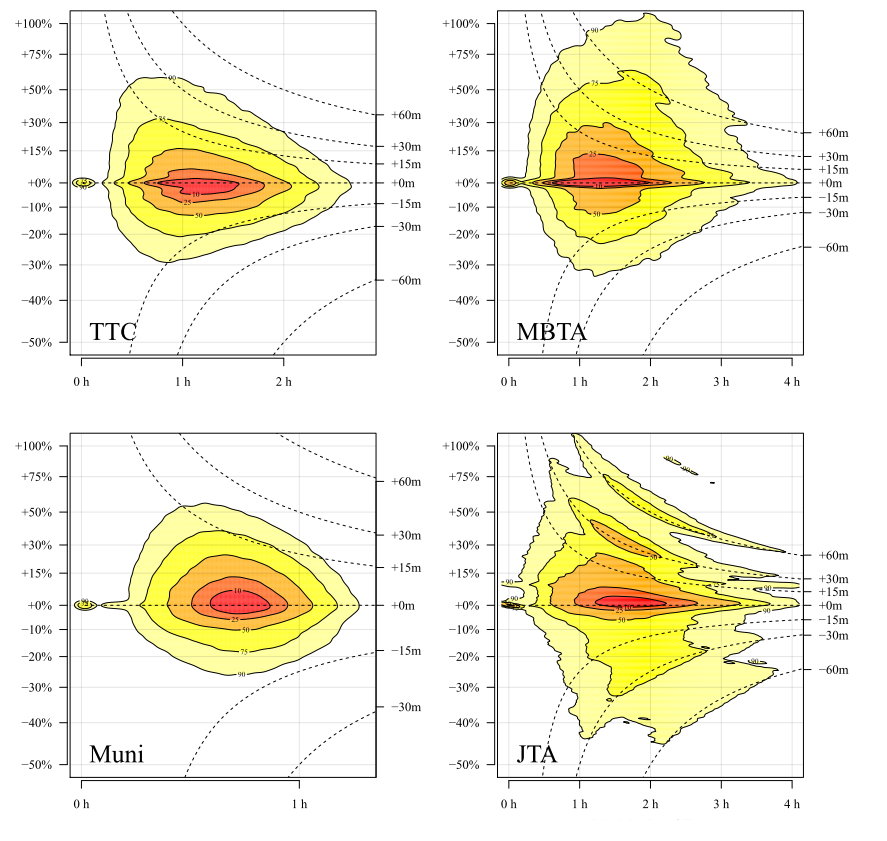
\includegraphics[width=16cm, keepaspectratio]{figure/2-wessel2019_aderencia.png}}
  }{
  \Fonte{Adaptada de Wessel (2019)}
  }
  \end{figure}
  
  No SIT-FOR, a agência de transporte fornece para o Google (que é quem faz o processamento final do GTFS) informações de horários programados somente do começo e do fim de cada viagem, que são os horários que são utilizados pela ETUFOR para o controle e operação do sistema. A informação de tempo de viagem de cada veículo entre paradas, que é uma informação necessária nesse formato de GTFS, não é fornecida, ficando ao cargo do Google a estimação. O método utilizado pela empresa é desconhecido.
  
  Portanto, a literatura aponta para a necessidade de métodos e dados para melhorar a qualidade dos dados de GTFS, por conseguinte aprimorando a estimação de tempos de viagem entre pares origem-destino e o cálculo de indicadores de acessibilidade. Para esse fim, dados de localização da frota (AVL) e bilhetagem (\emph{smartcard}) podem ser utilizados.
  
  \hypertarget{como-o-big-data-pode-ajudar-na-estimacao}{%
  \subsection{Como o big data pode ajudar na estimação?}\label{como-o-big-data-pode-ajudar-na-estimacao}}
  
  Como já foi visto no começo do capítulo, dados de GPS são usados principalmente para o controle do sistema e estimação de indicadores operacionais de desempenho. Apesar de incipiente, esforços têm sido feitos para incorporar dados de localização da frota na melhoria da estimação de indicadores de acessibilidade por transporte público. Os métodos desses trabalhos buscam transformar dados brutos de localização da frota em uma tabela de horários dos veículos no estilo \emph{stop\_times.txt} do GTFS.
  
  Destaca-se o trabalho de \citet{Wessel2017}, que utilizou dados de GPS de Toronto, Canadá, para corrigir os dados de GTFS. Os dados de GPS eram disponibilizados em tempo real através de uma API do serviço \emph{NextBus}, que automaticamente detecta a linha, o sentido, e quando havia o fim de uma viagem e começo de outra. O algoritmo desenvolvido pelos autores coletou dois dias de registro, e primeiramente buscou detectar erros nessas informações. Em seguida, os autores estabeleceram um \emph{buffer} de 20 metros em relação a cada parada (coletada a partir do GTFS da cidade) para estabelecer o ponto de GPS (e a hora), estimando os tempos de parada de cada viagem.
  
  Com a estimação do tempo de parada de cada viagem feita (e já com as informações de linha, sentido, e veículo), o novo arquivo já era análogo ao arquivo agendado \emph{stop\_times.txt}, e foi utilizado para o roteamento pelo \emph{OpenTripPlanner} e a estimação do tempo de viagem entre pares origem destino (no caso, setores censitários). Por fim, foram calculados indicadores de acessibilidade cumulativa para empregos em até 45 minutos de viagem antes e depois da correção.
  
  Os autores demonstraram que muitas vezes o horário agendado das viagens do transporte público da cidade é conservador, levando à subestimação do indicador de acessibilidade. A principal conclusão do estudo, entretanto, é que a variação entre o horário agendado e real parece não ser aleatória, afetando diferentemente certas regiões da cidade (Figura \ref{fig:wessel-2017}).
  
  \begin{figure}[!h]
  \captionsetup{width=16cm}
  \Caption{\label{fig:wessel-2017}Diferença relativa de acessibilidade entre acessibilidade programada e corrigida}
  \centering
  \UFCfig{}{
  {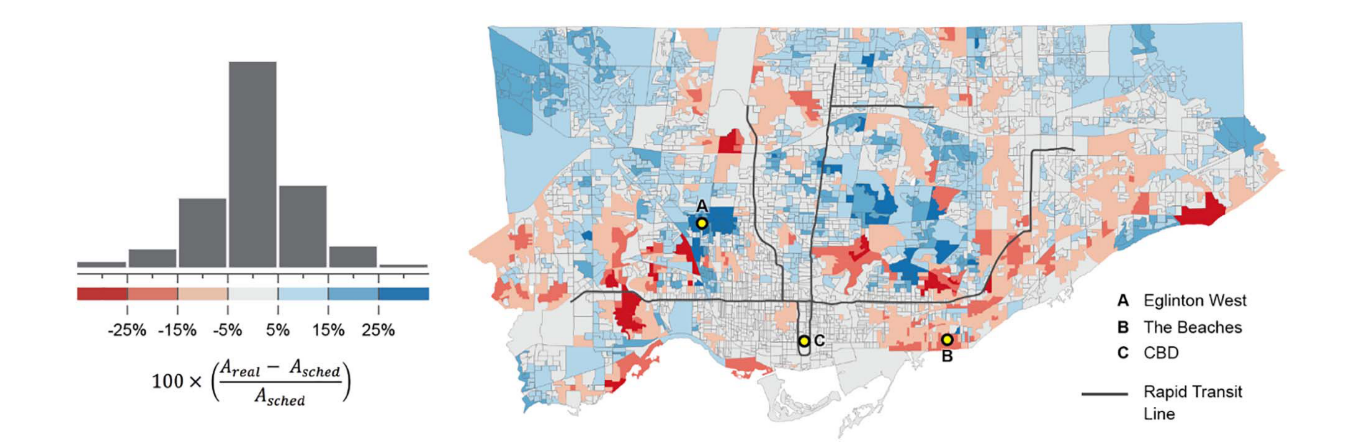
\includegraphics[width=16cm, keepaspectratio]{figure/2-wessel_2017.png}}
  }{
  \Fonte{Adaptada de Wessel (2017)}
  }
  \end{figure}
  
  Com um objetivo de trabalho diferente, \citet{Arbex2016a} também utilizaram de dados de GPS para corrigir os arquivos de GTFS para o sistema de transporte público de São Paulo. A metodologia de transformação dos dados de GPS em dados \emph{stop\_times.txt} de GTFS não foi detalhada, mas entendeu-se que o autor adaptou a mesma metodologia do seu trabalho anterior \citep{Arbex2016}.
  
  Neste trabalho, com um objetivo de fazer análise \emph{ex-post} de faixas exclusivas, os autores utilizaram 20 dias úteis de agosto de 2013 (sem faixa exclusiva) e 20 dias úteis de abril de 2015 (com faixas exclusivas) de dados de GPS arquivados. O trabalho propôs fazer uma integração com os dados de oferta do sistema disponíveis no arquivo de GTFS, agregando os registros de GPS a cada parada de ônibus, sem interpolação linear. A metodologia de geoprocessamento dos dados de GPS proposta respeitou, resumidamente, as seguintes etapas:
  
  \begin{itemize}
  \tightlist
  \item
    \textbf{Leitura dos dados}: os dados referentes aos registros de GPS e às paradas de ônibus servidas por cada linha (\emph{stops.txt} e \emph{stop\_times.txt} dos dados de GTFS) foram armazenados;
  \item
    \textbf{Filtro espacial}: registros de GPS que erroneamente foram localizados fora da cidade de São Paulo foram excluídos;
  \item
    \textbf{Ordenação}: os dados de GPS são ordenados por linha, veículo e hora;
  \item
    \textbf{Associação ao ponto de ônibus mais próximo}: cada registro de GPS foi alocado à parada mais próxima, de acordo com a linha em questão;
  \item
    \textbf{Filtro espacial}: registros de GPS que apresentaram uma distância maior que 200 metros da parada mais próxima foram descartados;
  \item
    \textbf{Separação de viagens}: viagens diferentes são identificadas através de uma diferença abrupta entre as paradas do registro do GPS: se em um registro (já ordenado por linha e por hora) foi identificado a parada 88 da linha e no registro seguinte foi registrada a parada 2, determina-se que houve uma mudança de viagem;
  \item
    \textbf{Correção das viagens}: a correção envolveu interpolação quando houve parada sem um registro de GPS, quando houve alguma inconsistência na rota do ônibus, ou quando houve dados repetidos devido à parada do veículo.
  \end{itemize}
  
  A principal limitação identificada no trabalho foi o método para estimar o tempo de passagem de cada veículo pelas paradas da linha. O autor associou o registro de GPS mais próximo de cada parada como sendo o horário associado, utilizando um limite de 200 metros (em distância euclidiana) para julgar se aquela associação foi válida ou não. Isso significa que um registro de GPS com até 200 metros de distância da parada pode ser utilizado, o que pode acarretar erros de estimação.
  
  Outra limitação do método de tratamento dos dados de GPS foi que, para evitar problemas, o autor não considerou as paradas extremas (de fim e de começo da viagem). Isso pode ser problemático especialmente em áreas de terminais, onde há um grande fluxo de veículos e onde atrasos e altos tempos de viagem são comuns.
  
  Com isso, o autor pôde estimar tempos de viagem (entre zonas de tráfego) com o uso do software \emph{ArcGis} e calcular e analisar indicadores de acessibilidade, mas não fez uma análise comparativa da acessibilidade com o GTFS programado e com o GTFS empírico.
  
  No que se refere à fonte de dados, a principal diferença entre os trabalhos de \citet{Wessel2017} e \citet{Arbex2016a} está no fato de que o primeiro contou com dados de GPS que eram coletados em tempo real de um serviço, através de uma API, que já contava com informações de viagem e sentido da linha, enquanto que o último contou com dados arquivados de GPS, com mais carência de informações. Essa diferença levou o trabalho de \citet{Arbex2016a}, na tentativa de obter informações já disponíveis ao trabalho de \citet{Wessel2017}, a adotar uma metodologia de geoprocessamento dos dados de GPS mais extensa e elaborada, trazendo mais contribuições para a aŕea.
  
  O serviço de dados de GPS utilizado por \citet{Wessel2017} está presente em mais de 50 cidades, porém concentrado nos Estados Unidos, Canadá e Austrália (informação coletada em agosto de 2019 no site \url{https://nextbus.cubic.com/Our-Customers/Around-the-World}). Identifica-se, portanto, que a metodologia desenvolvida no trabalho de \citet{Arbex2016a} pode ser mais útil para a realidade dos demais países (especialmente países emergentes), onde a tendência é a disponibilização de dados de GPS arquivados e carentes de informações.
  
  Outro aspecto importante a ser ressaltado é como foi feita a agregação temporal dos dados. \citet{Wessel2017} teve acesso a localização de todos os veículos do sistema por 2 dias, com exceção das linhas de alta capacidade, que o autor utilizou os dados programados. Então calcularam a acessibilidade para o serviço observado nesses dias, por fim fazendo uma acessibilidade média dessa amostra. \citet{Arbex2016a} aplicaram seu algoritmo para 20 dias úteis, mas não foi explicitado como os tempos estimados entre paradas foram agregados.
  
  Esses são os trabalhos encontrados que realizaram uma transformação de dados de localização da frota em dados \emph{stop\_times} do GTFS, trazendo informações empíricas de tempo de viagem. Outros trabalhos, apesar de não terem feito uma tradução completa dos dados de GPS em dados \emph{stop\_times}, propuseram métodos para geoprocessar dados de GPS com uso dos dados de GTFS, estimando informações importantes de serviço. Como exemplo, destaca-se o trabalho de \citet{Rabay2017}, que utilizou os dados de GPS para estimar velocidades operacionais em trechos de algumas linhas, e merece uma atenção especial.
  
  Ao contrário dos dados de GPS utilizado nos estudos de \citet{Wessel2017} e \citet{Arbex2016}, os dados de AVL do SIT-FOR não possuem a informação da linha em que o carro está operando. Além disso, o número do veículo na base do GPS é diferente do número do veículo na base da bilhetagem. Com isso em mente, o trabalho de \citet{Rabay2017}, com o objetivo de estimar indicadores operacionais, propôs uma metodologia para identificar linha, sentido e viagem na base do GPS. Primeiramente, fazendo o uso de um dicionário de equivalência entre o número do carro nos dados de AVL e bilhetagem, o autor transpôs a coluna da linha da base da bilhetagem para a base do GPS. Em seguida, o autor utilizou os itinerários das linhas (a partir dos dados GTFS) para criar uma área de influência de cada uma delas. Dessa forma, pôde manter somente os registros de GPS que estavam contidos nas áreas de influência das linhas correspondente, eliminando pontos em trajetos fora da linha, que acontecem quando o veículo está indo pra garagem ou quando um mesmo carro serve a mais de uma linha.
  
  Para determinar o sentido de cada viagem, o autor assumiu que todas as viagens que aconteciam eram no sentido da ida, e fez um snap de cada ponto de GPS para a linha do sentido de ida. Com isso, calculou a distância acumulada que o veículo percorria. Quando a distância acumulada aumentava, significava que o veículo estava indo no sentido da linha, ou seja, ida. Quando a distância diminuía, significava que estava voltando. Após alguns testes de qualidade, o autor dividiu a linha em diversos trechos e fez o snap dos pontos de GPS para esses trechos, podendo assim calcular indicadores operacionais.
  
  Entretanto, o método não levou em consideração o tempo perdido no final e começo das linhas. Especialmente em terminais de integração fechados, leva-se muito tempo para manobrar e embarcar os usuários e, em certas situações, o veículo apresenta um tempo ocioso, sem operar. A não consideração desse aspecto pode fazer com que aconteça um erro na estimação da velocidade de operação. Além disso, a metodologia foi aplicada somente para um dia e 4 linhas, não sendo testada para todo o sistema de transporte público onde há diversas situações que podem tornar o método proposto impreciso.
  
  \hypertarget{e-como-os-dados-de-bilhetagem-podem-ajudar}{%
  \subsection{E como os dados de bilhetagem podem ajudar?}\label{e-como-os-dados-de-bilhetagem-podem-ajudar}}
  
  Como acontece com a utilização de GPS na estimação de indicadores de acessibilidade, a utilização de dados de bilhetagem recebe pouca atenção na literatura. O mesmo trabalho de \citet{Arbex2016a} analisado na seção anterior também fez uma análise utilizando dados de bilhetagem, onde os autores selecionaram cinco bairros de baixa renda de São Paulo e estimaram o tempo de viagem (motivo trabalho) de cada usuário do transporte público a partir dos dados de \emph{smartcard}. Junto com a análise de um indicador cumulativo de acessibilidade, os autores analisaram os percentis 50 e 90 dos tempos de viagem estimados. Em seguida, utilizaram o percentil 90 do tempo de viagem estimado de cada um dos bairros como o time threshold para o indicador cumulativo de acessibilidade, analisando a porcentagem de empregos acessíveis nesse tempo.
  
  A utilização dos tempos de viagem a partir da bilhetagem para estabelecer limites de tempo em um indicador cumulativo vai de encontro à discussão proposta por \citet{Paez2012} de acessibilidade normativa vs acessibilidade positiva. A acessibilidade normativa é implementada baseada em valores de distância ou tempo de viagem que são assumidos pelos autores, como, por exemplo, o tempo limite (\emph{time threshold}) de acesso a oportunidades para um indicador cumulativo. A acessibilidade positiva é baseada no comportamento dos usuários para definir esses parâmetros de distância ou tempo de viagem, como, por exemplo, a utilização de uma matriz origem destino para calibrar um modelo gravitacional, ou o uso do tempo de viagem coletado em pesquisas para definir o tempo limite em indicadores cumulativos.
  
  Os autores ainda argumentam que a diferença entre uma acessibilidade normativa e positiva pode ser significativa. Além disso, valores assumidos de tempo de viagem limite podem depender da cidade, atividade, grupo social, etc. \citet{Pereira2019} mostra, por exemplo, como uma análise de diferença de acessibilidade por faixa de renda pode mudar a conclusão dependendo do tempo limite utilizado no indicador cumulativo.
  
  Por fim, o único trabalho encontrado que utilizou dados de big data de transporte público para a implementação de uma acessibilidade positiva foi o de \citet{Arbex2016a}. Falta na literatura ainda a consolidação de um método para a utilização desses dados para esses fins, e a diferença que eles trariam em comparação à utilização de valores normativos.
  
  \hypertarget{consideracoes-finais}{%
  \section{Considerações finais}\label{consideracoes-finais}}
  
  O primeiro tópico da revisão mostrou os principais usos do \emph{big data} no planejamento de transporte público. Em seguida, métodos de consolidação e integração das bases de dados foram abordados. Um destaque especial foi dado ao geoprocessamento dos dados de GPS, principalmente na sua integração com os dados de GTFS. Algumas lacunas desta etapa foram identificadas e analisadas, tendo em vista que estão presentes na problemática deste trabalho.
  
  O segundo tópico começou com uma introdução do conceito de acessibilidade, com os seus componentes e tipos. Em seguida, foi analisado o desenvolvimento dos métodos de estimação dos indicadores por transporte público ao longo dos anos, que culminou na utilização de dados padronizados da oferta de transporte público para a estimação do componente de transporte da acessibilidade. Esses dados, entretanto, apresentam problemas de confiabilidade devido ao fato de serem programados pela agência de transporte. Assim, foram analisadas as metodologias que já foram desenvolvidas para a correção desses horários programados com o uso de dados de localização da frota. Só o trabalho de \citet{Wessel2017} focou em um método para a transformação de uma base de dados de GPS para um arquivo \emph{stop\_times.txt}, mostrando a importância de fazer essa transformação. Entretanto, foi identificado que os dados de GPS do trabalho são diferentes de dados de GPS arquivados comumente encontrados (inclusive do SIT-FOR). Dentro da realidade dos arquivos GPS arquivados, foram identificados alguns trabalhos que propuseram metodologias de utilização de dados de GTFS no tratamento de dados de GPS, mas com objetivos distintos.
  
  No que diz respeitos às hipóteses levantadas nas questões de pesquisa, a primeira hipótese foi abordada pelo trabalho de \citet{Wessel2017}, mas entende-se que é necessário avançar nessa verificação e nas implicações que ela tem para a tomada de decisão e avaliação de alternativas.
  
  Para a segunda hipótese, foi identificada uma lacuna no que dizia respeito à utilização da amostra advinda dos dados de GPS. Os trabalhos encontrados utilizaram amostras de mais de um dia, mas no fim acabaram fazendo a média dos valores, de uma forma ou de outra. É entendido que as amostras coletadas podem ser utilizada para mais que uma análise mediana do sistema, principalmente em cenários onde o tempo de viagem por transporte público pode ser tão variável.
  
  Para a terceira hipótese, muitos trabalhos já analisaram essa varibilidade: \citet{Owen2015} introduziu o fenômeno, e mais recentemente \citet{Stepniak2019} fez uma revisão de boa parte dos trabalhos que já abordaram a temática. Algumas lacunas adicionais podem ser observadas, como as atividades consideradas e as resoluções espaciais utilizadas.
  
  Por fim, do lado dos dados de bilhetagem, foi identificada uma lacuna na utilização de dados de \emph{smartcard} na estimação de indicadores positivos. \citet{Arbex2016a} propôs uma utilização para esses fins, mas entende-se que ainda é preciso discutir a utilização e consolidar métodos para tal.
  
  Os métodos desenvolvidos neste trabalho então buscam abordar essas lacunas de pesquisa. Primeiramente, é necessário preparar os dados do transporte público de Fortaleza para em seguida estabelecer os métodos. A consolidação e integração dos dados se propõe a isso.
  
  \hypertarget{consolidacao-e-integracao-dos-dados-do-sit-for}{%
  \chapter{Consolidação e Integração dos dados do SIT-FOR}\label{consolidacao-e-integracao-dos-dados-do-sit-for}}
  
  A consolidação tem como objetivo fazer uma apresentação, preparar os dados para a sua disponibilização e para as etapas seguintes de estimação de indicadores de acessibilidade. O capítulo começa com uma contextualização do SIT-FOR. Em seguida, a consolidação proposta neste trabalho divide o processo em duas etapas principais: tratamento inicial dos dados e integração das bases. As bases utilizadas são: bilhetagem, GPS, cadastro dos usuários e GTFS. Por fim, são mostrados os resultados da consolidação, com as limitações amostrais ocasionadas pela integração das bases.
  
  \hypertarget{sistema-de-transporte-publico-integrado-de-fortaleza-sit-for}{%
  \section{Sistema de Transporte Público Integrado de Fortaleza (SIT-FOR)}\label{sistema-de-transporte-publico-integrado-de-fortaleza-sit-for}}
  
  A expansão da malha urbana de Fortaleza é mostrada na Figura \textbackslash{}ref\{fig:fortaleza-crescimento). Observa-se que a cidade começou a se desenvolver no centro, expandindo sua mancha urbana (em preto) para os bairros periféricos. De acordo com dados do Censo, Fortaleza cresceu de 270 mil habitantes em 1950 para quase 2 milhões e 500 mil habitantes em 2010 \citep{Fortaleza2040}. Essa expansão trouxe grandes desafios aos planejadores da cidade no que se refere aos transporte dessa nova massa de habitantes.
  
  \begin{figure}[!h]
  \captionsetup{width=16cm}
  \Caption{\label{fig:fortaleza-crescimento}Expansão Urbana de Fortaleza}
  \centering
  \UFCfig{}{
  {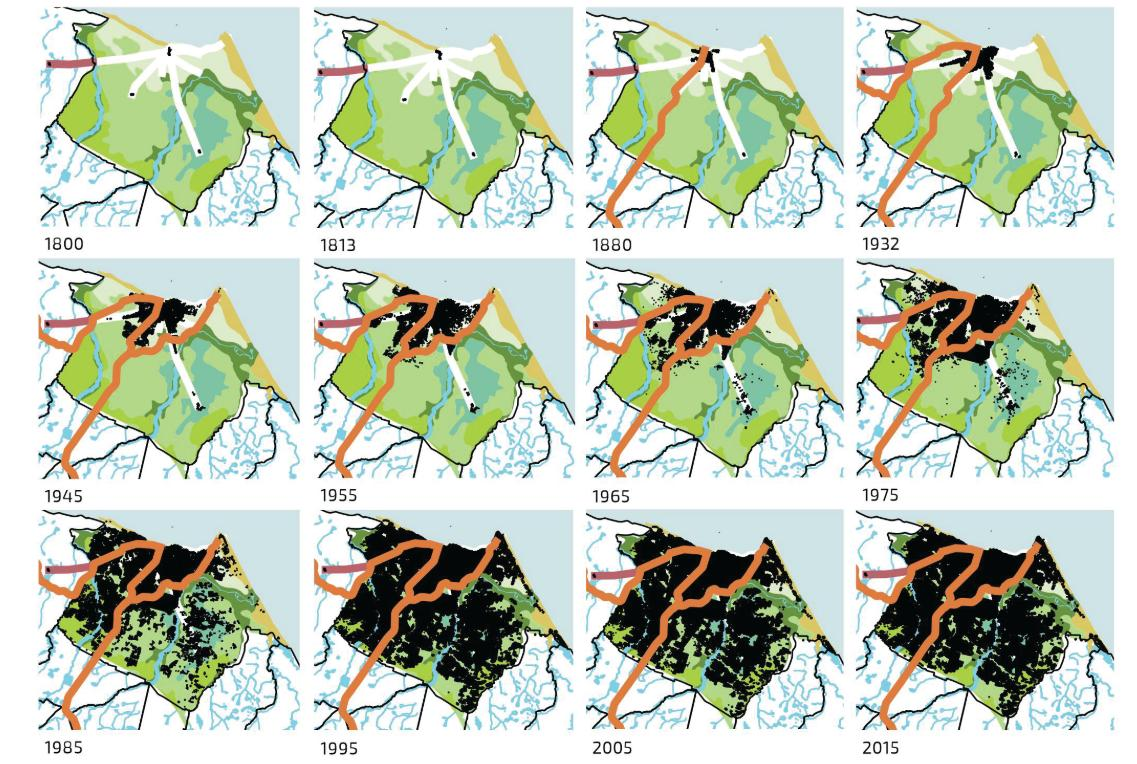
\includegraphics[width=16cm, keepaspectratio]{figure/3-fortaleza_expansao.jpg}}
  }{
  \Fonte{Fortaleza 2040}
  }
  \end{figure}
  
  Após tentativas frustradas de organização dos serviços de transporte público, em 1992 foi criado o Sistema Integrado de Transportes de Fortaleza (SIT-FOR) pela então Empresa de Trânsito e Transporte Urbana S/A - ETUSA. O novo sistema de transporte público estabeleceu uma configuração tronco-alimentadora de operação, com a criação de terminais de integração fechados nos bairros e terminais abertos no Centro. As linhas alimentadoras levam os passageiros dos bairros até os terminais, e as linhas troncais levariam os passageiros dos terminais até a área central da cidade. Além disso, linhas complementares, circulares e inter bairros também foram implementadas \citep{Fortaleza2015}. A Figura \ref{fig:fortaleza-linhas} mapeia a configuração espacial do sistema. No mapa não estão presentes as linhas de transporte de alta capacidade (trem e VLT). Essas linhas ainda não estão operacionalmente e tarifariamente integradas ao sistema de ônibus de Fortaleza, além de apresentarem uma operação que está longe da sua capacidade. A Linha Sul opera em um intervalo de aproximadamente 15 minutos entre trens, a Linha Oeste em cerca de 30 minutos, e a linha do VLT está em operação assistida.
  
  \begin{figure}[!h]
  \captionsetup{width=16cm}
  \Caption{\label{fig:fortaleza-linhas}Linhas troncais e alimentadoras do SIT-FOR}
  \centering
  \UFCfig{}{
  {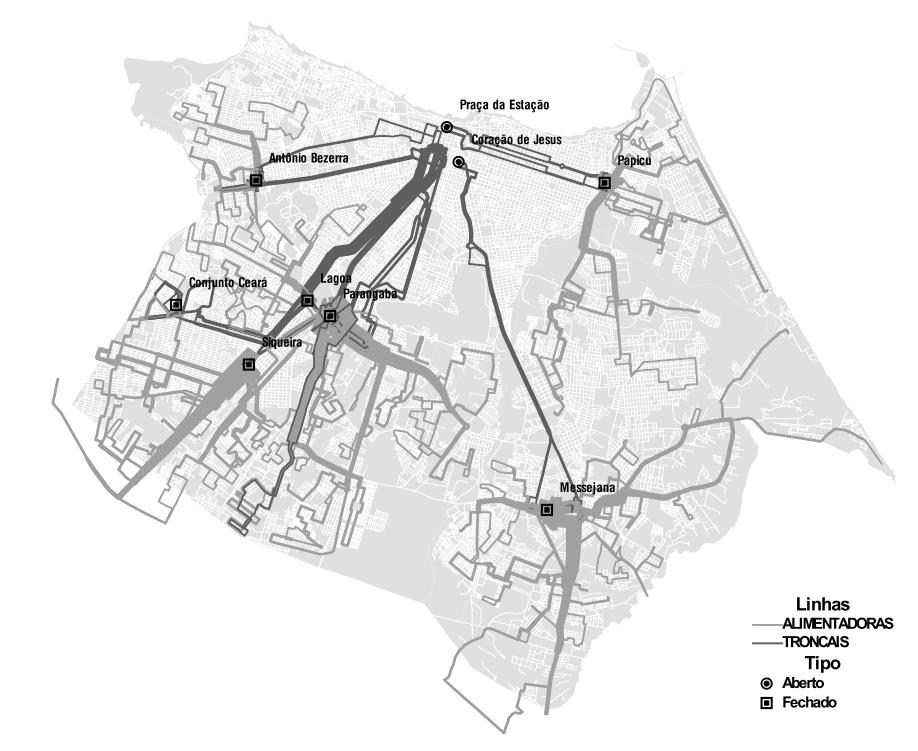
\includegraphics[width=16cm, keepaspectratio]{figure/3-sitfor.jpg}}
  }{
  \Fonte{Fortaleza (2010)}
  }
  \end{figure}
  
  No que se refere ao seu sistema que gera o \emph{big data}, O SIT-FOR têm um sistema aberto de bilhetagem eletrônica (usuários só validam no embarque) que registra a passagem de todos os usuários pela catraca dos veículos. Os tipos de pagamentos utilizados podem ser por bilhete único de vale transporte, carteira de estudante (mostrados na Figura \ref{fig:bu}), gratuidade de idosos, deficientes e funcionários, e inteira (pagamento por dinheiro). Já o sistema de \emph{Automated Vehicle Location} (Localização automática de veículos) consiste na presença de equipamentos de GPS em todos os veículos da frota de transporte público de Fortaleza. O sistema registra a localização de cada veículo em média a 30 segundos quando o veículo está ligado.
  
  \begin{figure}[!h]
  \captionsetup{width=16cm}
  \Caption{\label{fig:bu}Cartões de Bilhetagem Eletrônica do SIT-FOR}
  \centering
  \UFCfig{}{
  {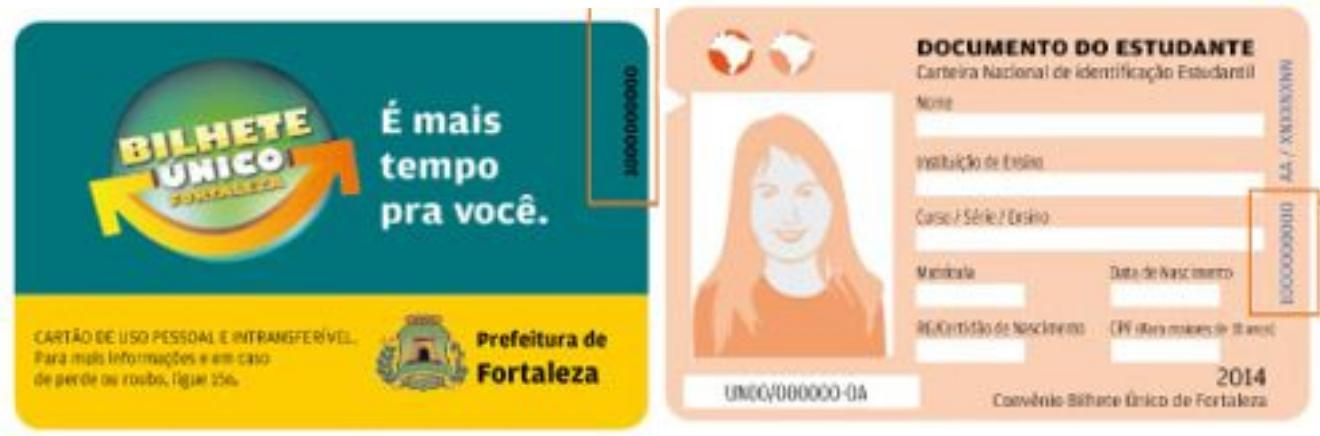
\includegraphics[width=16cm, keepaspectratio]{figure/3-bu.jpg}}
  }{
  \Fonte{Prefeitura de Fortaleza}
  }
  \end{figure}
  
  \hypertarget{metodo-de-tratamento-inicial-dos-dados}{%
  \section{Método de tratamento inicial dos dados}\label{metodo-de-tratamento-inicial-dos-dados}}
  
  O tratamento inicial dos dados busca converter os dados brutos para um formato sem informações desnecessárias e com as colunas nomeadas. A Figura \ref{fig:cons-tratamento-inicial} descreve as principais etapas.
  
  \begin{figure}[!h]
  \captionsetup{width=16cm}
  \Caption{\label{fig:cons-tratamento-inicial}Tratamento inicial dos dados}
  \centering
  \UFCfig{}{
  {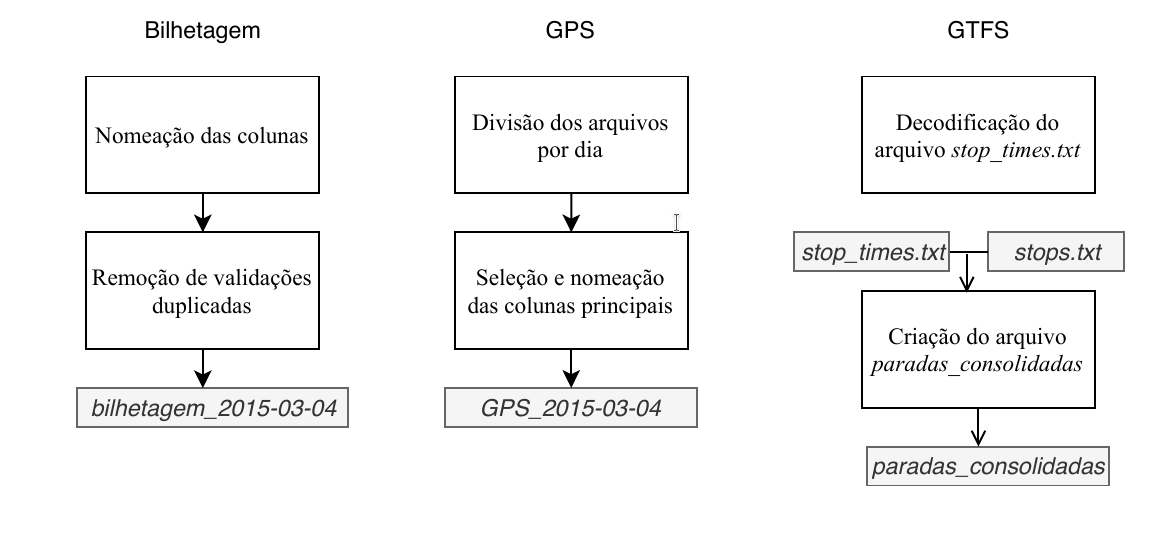
\includegraphics[width=16cm, keepaspectratio]{figure/3-tratamento_inicial.png}}
  }{
  \Fonte{Elaborada pelo autor}
  }
  \end{figure}
  
  \hypertarget{dados-de-bilhetagem}{%
  \subsection{Dados de bilhetagem}\label{dados-de-bilhetagem}}
  
  Os dados brutos de bilhetagem contém 9 colunas, sendo originalmente divididos por dia. Por meio de informações fornecidas pelo órgão fornecedor dos dados, foi possível nomear as colunas de acordo com o seu conteúdo:
  
  \begin{itemize}
  \tightlist
  \item
    \emph{id}: representa o código Siom do usuário, que é o código que identifica o usuário do cartão;
  \item
    \emph{linha}: representa o código da linha onde aconteceu a validação;
  \item
    \emph{nome\_linha}: representa o nome da linha;
  \item
    \emph{prefixo\_carro}: numero do veículo de acordo com a ETUFOR;
  \item
    \emph{hora}: a hora e o dia da validação, no formato ISO 8601 ano/mês/dia hora:minuto:segundo;
  \item
    \emph{tipo\_cartao}: código do tipo de cartão utilizado;
  \item
    \emph{nome\_cartao}: nome do tipo de cartão utilizado;
  \item
    \emph{sentido\_viagem}: o sentido da viagem (ida ou volta);
  \item
    \emph{integracao}: se a viagem foi uma integração ou não.
  \end{itemize}
  
  A coluna tipo\_cartao contém 9 tipos de pagamento diferentes. É simplificada para quatro tipos principais: \emph{vale transporte}, \emph{carteira de estudante}, \emph{gratuidade} e \emph{inteira}. As colunas \emph{nome\_linha} e \emph{nome\_cartao} são removidas por conterem informações correspondentes nas colunas \emph{linha} e \emph{tipo\_cartao}. A Tabela \ref{tab:bi_sample} apresenta uma amostra desses dados já com a nomeação das colunas.
  
  \begin{table}[!h]
  \captionsetup{width=16cm}%Deixe da mesma largura que a tabela
  \Caption{\label{tab:bi_sample} Amostra da base da bilhetagem}%
  \IBGEtab{}{%
      \begin{tabular}{ccccccc}
          \toprule
          id & linha & prefixo\_carro & hora & tipo\_cartao & sentido\_viagem & integracao\\
          \midrule
          6626108 & 84 & 2007 & 2018-08-04 20:16:47 & Vale Transporte & Volta & S\\
      5488895 & 84 & 2007 & 2018-08-04 18:01:00 & Vale Transporte & Ida & S\\
      7173980 & 84 & 2007 & 2018-08-04 18:10:03 & Estudante & Ida & N\\
      4818496 & 84 & 2007 & 2018-08-04 18:16:54 & Vale Transporte & Ida & N\\
      7400045 & 84 & 2007 & 2018-08-04 17:27:54 & Vale Transporte & Volta & N\\
      3834561 & 84 & 2007 & 2018-08-04 17:37:07 & Estudante & Volta & N\\
      5300990 & 84 & 2007 & 2018-08-04 17:42:56 & Vale Transporte & Volta & N\\
      4616189 & 84 & 2007 & 2018-08-04 16:09:59 & Vale Transporte & Ida & N\\
      2674363 & 84 & 2007 & 2018-08-04 15:00:24 & Estudante & Ida & N\\
      2835333 & 84 & 2007 & 2018-08-04 14:04:42 & Gratuidade & Volta & N\\
          \bottomrule
      \end{tabular}%
  }{%
  \Fonte{Elaborada pelo autor}%
    }
    \end{table}
  
  Em seguida, é feita a remoção de dados duplicados. Isso acontece quando o usuário erroneamente passa o seu cartão mais de uma vez, ou quando um usuário do cartão passa o cartão para diversos usuários. Para isso, validações de um mesmo usuário na mesma linha em um intervalo menor que 5 minutos entre elas serão removidas, mantendo somente a primeira validação.
  
  \hypertarget{dados-de-gps}{%
  \subsection{Dados de GPS}\label{dados-de-gps}}
  
  Cada veículo da frota de transporte público de Fortaleza é rastreado por um aparelho de GPS. Na maioria dos casos o aparelho registra a localização de cada veículo a cada 30 segundos. No total, cada registro desse de localização do veículo apresenta mais de 40 atributos (colunas), sendo grande parte vazios ou nulo.
  
  Os dados brutos são fornecidos por mês, com cada arquivo ocupando cerca de 7,5 GB de espaço em disco e contendo cerca de 125 milhões de linhas. Para facilitar o manejo dos dados em um computador com poder de processamento médio, esses arquivos foram divididos por dia em um computador de processamento maior (\textgreater{} 16 GB de memória e 4+ núcleos). Por fim, foram mantidas somente as colunas que apresentavam informações necessárias:
  
  \begin{itemize}
  \tightlist
  \item
    \emph{vehicleid}: a identificação do veículo de acordo com o estabelecido pela empresa;
  \item
    \emph{hora}: o dia e a hora exata da localização registrada;
  \item
    \emph{lat}: a latitude onde se encontra o veículo;
  \item
    \emph{lon}: a longitude.
  \end{itemize}
  
  Uma inspeção na base de dados mostrou alguns problemas que precisavam ser resolvidos. O mais grave dizia respeito a hora de cada registro. Primeiro, foram identificados dois formatos de data diferentes: um no formato \texttt{anomesdiahoraminutosegundo} (aaaammddHHMMSS) e outro no formato de data UNIX, que apresenta a quantidade de segundos passados em relação a certa data (geralmente em relação ao dia 1970-01-01 00:00:00). Enquanto o problema do primeiro formato é de resolução rápida (basta mudar o formato organizando o ano, dia, etc), o problema do segundo foi de difícil resolução porque não fazia sentido ser a quantidade de segundos a partir de 1970. Por meio de tentativa e erro foi identificado que o formato representava a quantidade de segundos passados desde a data 2000-01-01 00:00:00. A hipótese da correção foi confirmada por outras pessoas que já haviam tido contato com os dados.
  
  Outro problema com a hora foi encontrado. Quando se fazia um histograma da quantidade de registros de localização por hora, a concentração dos pontos era contra-intuitiva, com uma maior concentração de pontos próximo das 9h e das 20h. Foi identificado então que a hora dos dados brutos sofreu uma modificação indevida para o fuso UTM, que é o fuso no meridiano de Greenwich e 3 horas a mais que o fuso brasileiro.
  
  Esses problemas foram então resolvidos e os arquivos de GPS consolidados foram salvos por dia no formato \texttt{gps\_2018-08-dd.csv}. Uma amostra da base é mostrada na Tabela \ref{tab:gps_sample}
  
  \begin{table}[!h]
  \captionsetup{width=10cm}%Deixe da mesma largura que a tabela
  \Caption{\label{tab:gps_sample} Amostra da base do GPS}%
  \IBGEtab{}{%
      \begin{tabular}{ccccccc}
          \toprule
          vehicleid & hora & lon & lat\\
          \midrule
          34489 & 2018-09-03 23:59:58 & -38.53342 & -3.878622\\
      32739 & 2018-09-03 23:59:55 & -38.56847 & -3.778345\\
      32739 & 2018-09-03 23:59:55 & -38.56847 & -3.778345\\
      32739 & 2018-09-03 23:59:55 & -38.56847 & -3.778345\\
      32736 & 2018-09-03 23:59:46 & -38.56870 & -3.778106\\
      32649 & 2018-09-03 23:59:27 & -38.56826 & -3.777836\\
      34489 & 2018-09-03 23:59:26 & -38.53342 & -3.878622\\
      36569 & 2018-09-03 23:59:25 & -38.56858 & -3.778086\\
      32127 & 2018-09-03 23:59:16 & -38.54580 & -3.744650\\
      32127 & 2018-09-03 23:59:16 & -38.54580 & -3.744650\\
          \bottomrule
      \end{tabular}%
  }{%
  \Fonte{Elaborada pelo autor}%
    }
    \end{table}
  
  \hypertarget{dados-de-gtfs}{%
  \subsection{Dados de GTFS}\label{dados-de-gtfs}}
  
  A Especificação Geral de Feeds de Transporte Público (GTFS) estabelece um formato para compartilhamento de dados de transporte público pelas agências reguladoras. Esse dados, fornecidos para o Google, contém informações de horários, itinerários das linhas e tarifa, permitindo que a empresa faça uso desses dados nos seus produtos (como no Google Maps) para fornecer rotas, estimações de tempo e custo monetário para o usuário.
  
  O formato unificado apresenta os seguintes arquivos principais (Figura \ref{fig:tratamento_gtfs}):
  
  \begin{itemize}
  \tightlist
  \item
    \emph{stops.txt}: as paradas do sistema de transporte público e sua localização;
  \item
    \emph{routes.txt}: informações básicas de cada linha de transporte público;
  \item
    \emph{trips.txt}: as viagens realizadas por cada linha;
  \item
    \emph{stop\_times.txt}: o horário programado de chegada de cada veículo, em cada viagem, às paradas do sistema;
  \item
    \emph{shapes.txt}: os pontos que definem cada rota das linhas do sistema de transporte público.
  \end{itemize}
  
  \begin{figure}[!h]
  \captionsetup{width=16cm}
  \Caption{\label{fig:tratamento_gtfs}GTFS e suas colunas}
  \centering
  \UFCfig{}{
  {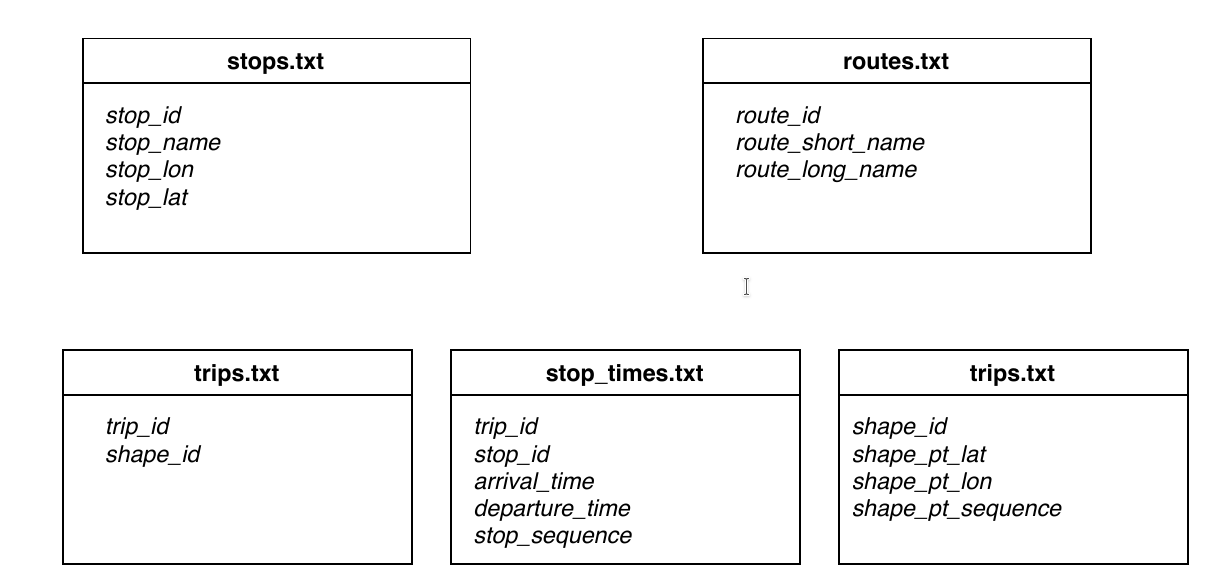
\includegraphics[width=16cm, keepaspectratio]{figure/3-tratamento_gtfs.png}}
  }{
  \Fonte{Elaborada pelo autor}
  }
  \end{figure}
  
  O tratamento inicial dos dados GTFS respeita as seguintes etapas:
  
  \begin{itemize}
  \tightlist
  \item
    \textbf{Decodificação da coluna \texttt{trip\_id} do arquivo \emph{stop\_times.txt}}: para identificar a linha, viagem, e sentido, é necessário decodificar a coluna em questão. Isso permitirá a adequação do arquivo;
  \item
    \textbf{Criação de uma tabela (\emph{paradas\_consolidadas}) com as paradas servidas por cada linha, sentido e sua sequência, georreferenciados}: é criado um novo arquivo a partir da junção do arquivo \emph{stop\_times.txt} modificado e o arquivo \emph{stops.txt} contendo todas as linhas, sentido, paradas, sequência e localização. Essa etapa é necessária para identificar a parada mais próxima de cada validação da bilhetagem;
  \item
    \textbf{Unificação dos pontos das linhas do arquivo \emph{shapes.txt} }: o arquivo contém ponto dos itinerários de cada linha de transporte público, então é proposto transformá-los em uma linestring para cada linha e sentido de viagem.
  \end{itemize}
  
  \hypertarget{dados-do-cadastro-do-bilhete-unico}{%
  \subsection{Dados do cadastro do bilhete único}\label{dados-do-cadastro-do-bilhete-unico}}
  
  O SIT-FOR registra informações dos usuários no momento que estes se registram para obtenção do bilhete único, e essas contém dados de identificação, endereço, data de nascimento, gênero e CEP. A identificação é a mesma presente na base da bilhetagem, permitindo uma integração entre os dados.
  
  A consolidação dessa base busca 1) renomear a coluna da identificação do bilhete único para o mesmo nome da bilhetagem (\texttt{id}); 2) transformar a data de nascimento em formato padrão ISO-8601 (ano-mes-dia hora:minuto:segundo).
  
  \hypertarget{metodo-proposto-de-integracao-da-base-da-bilhetagem-e-gps}{%
  \section{Método proposto de integração da base da bilhetagem e GPS}\label{metodo-proposto-de-integracao-da-base-da-bilhetagem-e-gps}}
  
  Há uma relação de dependência mútua dos dados de bilhetagem e GPS. Os dados de bilhetagem não apresentam a localização da validação, enquanto os dados de GPS não apresentam a linha que aquele veículo está servindo naquele ponto. Dessa forma, a integração permite utilizar os dados de GPS para determinar o local mais provável de cada validação na bilhetagem e permite utilizar os dados de bilhetagem para adicionar a informação da linha a qual aquele carro está servindo no GPS.
  
  Entretanto, como visto anteriormente, o número do veículo na bilhetagem (representado pela coluna \texttt{prefixo\_carro}) apresenta uma numeração diferente do número do veículo no GPS (coluna \texttt{vehicleid}). Para isso, existe uma base de dados aqui chamada de \texttt{dicionário}, que apresenta a relação de cada um dos \texttt{prefixo\_carro} para cada \texttt{vehicleid}.
  
  Foi determinado, então, que o método vai começar com a integração da bilhetagem com o dicionário (Figura \ref{fig:integracao_bases}). A base da bilhetagem contém a coluna \texttt{prefixo\_carro}, enquanto a base do GPS possui a coluna \texttt{vehicleid}, ambas representando a identificação do veículo em questão. O dicionário possui uma ``tradução'' dessas duas colunas, com um vehicleid para cada prefixo\_carro. É feito uma junção da bilhetagem com esse dicionário para criar a coluna \texttt{vehicleid} na base da bilhetagem.
  
  \begin{figure}[!h]
  \captionsetup{width=16cm}
  \Caption{\label{fig:integracao_bases}Integração das bases}
  \centering
  \UFCfig{}{
  {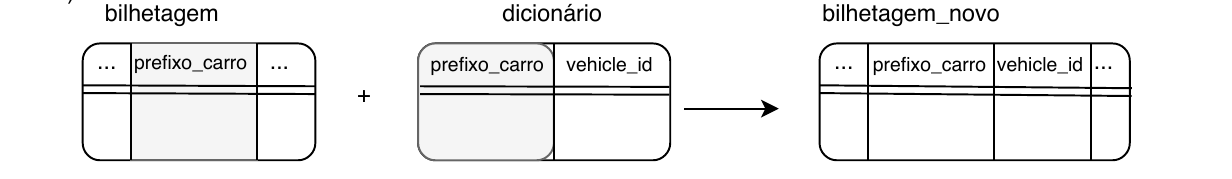
\includegraphics[width=16cm, keepaspectratio]{figure/3-integracao_bases.png}}
  }{
  \Fonte{Elaborada pelo autor}
  }
  \end{figure}
  
  \hypertarget{georreferenciamento-da-bilhetagem}{%
  \subsection{Georreferenciamento da bilhetagem}\label{georreferenciamento-da-bilhetagem}}
  
  Como a base da bilhetagem agora tem a coluna \texttt{vehicleid} igual ao do GPS, é possível ser feita a integração. Então, para o mesmo \texttt{vehicleid}, é buscado o momento mais próximo da bilhetagem na base do GPS. Com esse encontro feito, a coordenada aproximada do ônibus é extraída da base de GPS e integrada na base da bilhetagem (Figura \ref{fig:geo_bi}).
  
  \begin{figure}[!h]
  \captionsetup{width=16cm}
  \Caption{\label{fig:geo_bi}Georreferenciamento da bilhetagem}
  \centering
  \UFCfig{}{
  {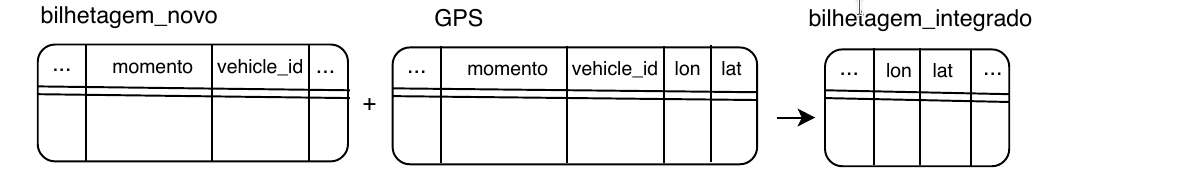
\includegraphics[width=16cm, keepaspectratio]{figure/3-geo_bilhetagem.png}}
  }{
  \Fonte{Elaborada pelo autor}
  }
  \end{figure}
  
  A base do GPS apresenta registros a 30 segundos, o que pode ocasionar algum erro na localização das validações. Além disso, é sabido que não há uma correspondência total entre os números de veículos das duas bases. O dicionário apresenta falhas que faz com que alguns carros da base da bilhetagem não tenham um carro equivalente na base do GPS, fazendo com que algumas validações não sejam georreferenciadas.
  
  Como exceção ao método desenvolvido nessa seção, dados referentes aos terminais são extraídos previamente e georreferenciados separadamente. Quando usuários entram a pé nos terminais fechados de integração, eles são requisitados a validar na entrada do local. Assim, os dados de bilhetagem registram o terminal em questão na coluna referente à linha.
  
  \hypertarget{integracao-da-informacao-da-linha-no-gps}{%
  \subsection{Integração da informação da linha no GPS}\label{integracao-da-informacao-da-linha-no-gps}}
  
  A utilização da base da bilhetagem para a determinação da linha no arquivo de GPS necessita de um método mais extenso, porque: 1) um mesmo carro pode servir a mais de uma linha no mesmo dia e 2) há diversos pontos registrados quando o veículo não está em serviço (indo e voltando da garagem, trocando de uma linha para outra, por exemplo).
  
  Para resolver o esses problemas, é proposta uma integração temporal das duas bases. É sabido que o mesmo carro pode servir a diferentes linhas em diferentes partes do dia. Assim, é criada uma tabela com o número do veículo, (\texttt{vehicleid}) a linha, e o horário que acontecia a primeira e a última validação naquela linha. Isso não representa o tempo total de viagem, visto que a viagem do veículo pode começar antes que o primeiro usuário valida (especialmente nos terminais de integração, onde não é feita a validação no veículo no começo da viagem), e pode acabar após que o último usuário valida. Portanto, é considerado que um intervalo para menos de 5 minutos, no caso do começo, e para mais de 5 minutos, no caso do fim da viagem, representa um intervalo que incorporará a viagem completa do veículo na linha. Esse método é aplicado para todas as linhas exceto corujão e expressos, porque essas apresentam um comportamento diferente do padrão.
  
  A junção das duas bases, portanto, terá como resultado a base do GPS com a coluna da linha correspondente, mantendo somente as observações onde o registro do GPS está inserido dentro do intervalo estipulado pela manipulação da base da bilhetagem. Esse procedimento resolve o problema dos veículos que servem a mais de uma linha no mesmo dia, mantendo somente as observações pertinentes a cada linha.
  
  É entendido que o intervalo estabelecido de 5 minutos minutos para mais e para menos pode ser excessivo, levando pontos fora da trajetória da linha (pontos de registro quando o veículo está indo para garagem, por exemplo) a serem incorporados na linha. Para isso, propõe-se uma etapa de validação com a utilização dos itinerários das linhas consolidados no arquivo \emph{shapes.txt} (um \textbf{filtro espacial}). Para cada linha do transporte público, é feito um buffer de 400 metros em torno do seu comprimento, definindo uma área de influência. Então, a base do GPS é dividida por linha e é feito uma determinação se cada registro está ou não inserido nos polígonos das linhas correspondentes. A Figura \ref{fig:integrar_gps_linha} mostra a presença de pontos fora da linha, que provavelmente são do deslocamento dos veículos até o terminal, e esses pontos são excluídos.
  
  \begin{figure}[!h]
  \captionsetup{width=16cm}
  \Caption{\label{fig:integrar_gps_linha}Área de influência e registros de GPS para uma linha}
  \centering
  \UFCfig{}{
  {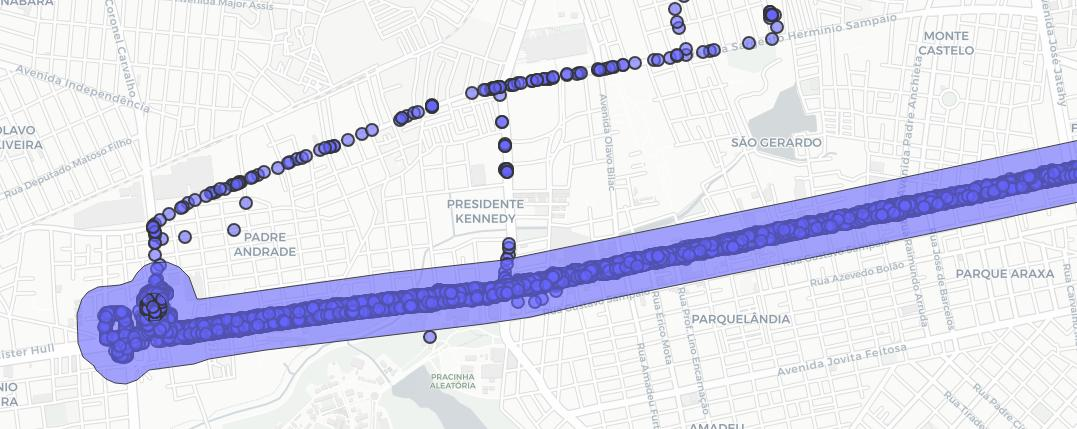
\includegraphics[width=16cm, keepaspectratio]{figure/3-integrar_gps_com_linha.jpg}}
  }{
  \Fonte{Elaborada pelo autor}
  }
  \end{figure}
  
  Além da área de influência das linhas, o ponto inicial e final de cada uma é identificado separadamente. Para as linhas que tem início ou fim no terminal de integração, um polígono com o terminal, extraído da base do \emph{OpenStreetMap}, é identificado (Figura \ref{fig:buffer_terminais}). Para as linhas que tem início ou fim fora do terminal, é determinado um círculo para representar o fim daquela linha. Esse procedimento tem como objetivo detectar quando o veículo chegou ao fim da linha, sendo assim possível determinar quando cada veículo terminou uma viagem e começou outra. Além disso, é possível estimar o tempo gasto com manobra no fim ou no começo da viagem.
  
  \begin{figure}[!h]
  \captionsetup{width=16cm}
  \Caption{\label{fig:buffer_terminais}Exemplo de polígonos dos terminais: Messejana (esquerda) e Papicu (direita)}
  \centering
  \UFCfig{}{
  {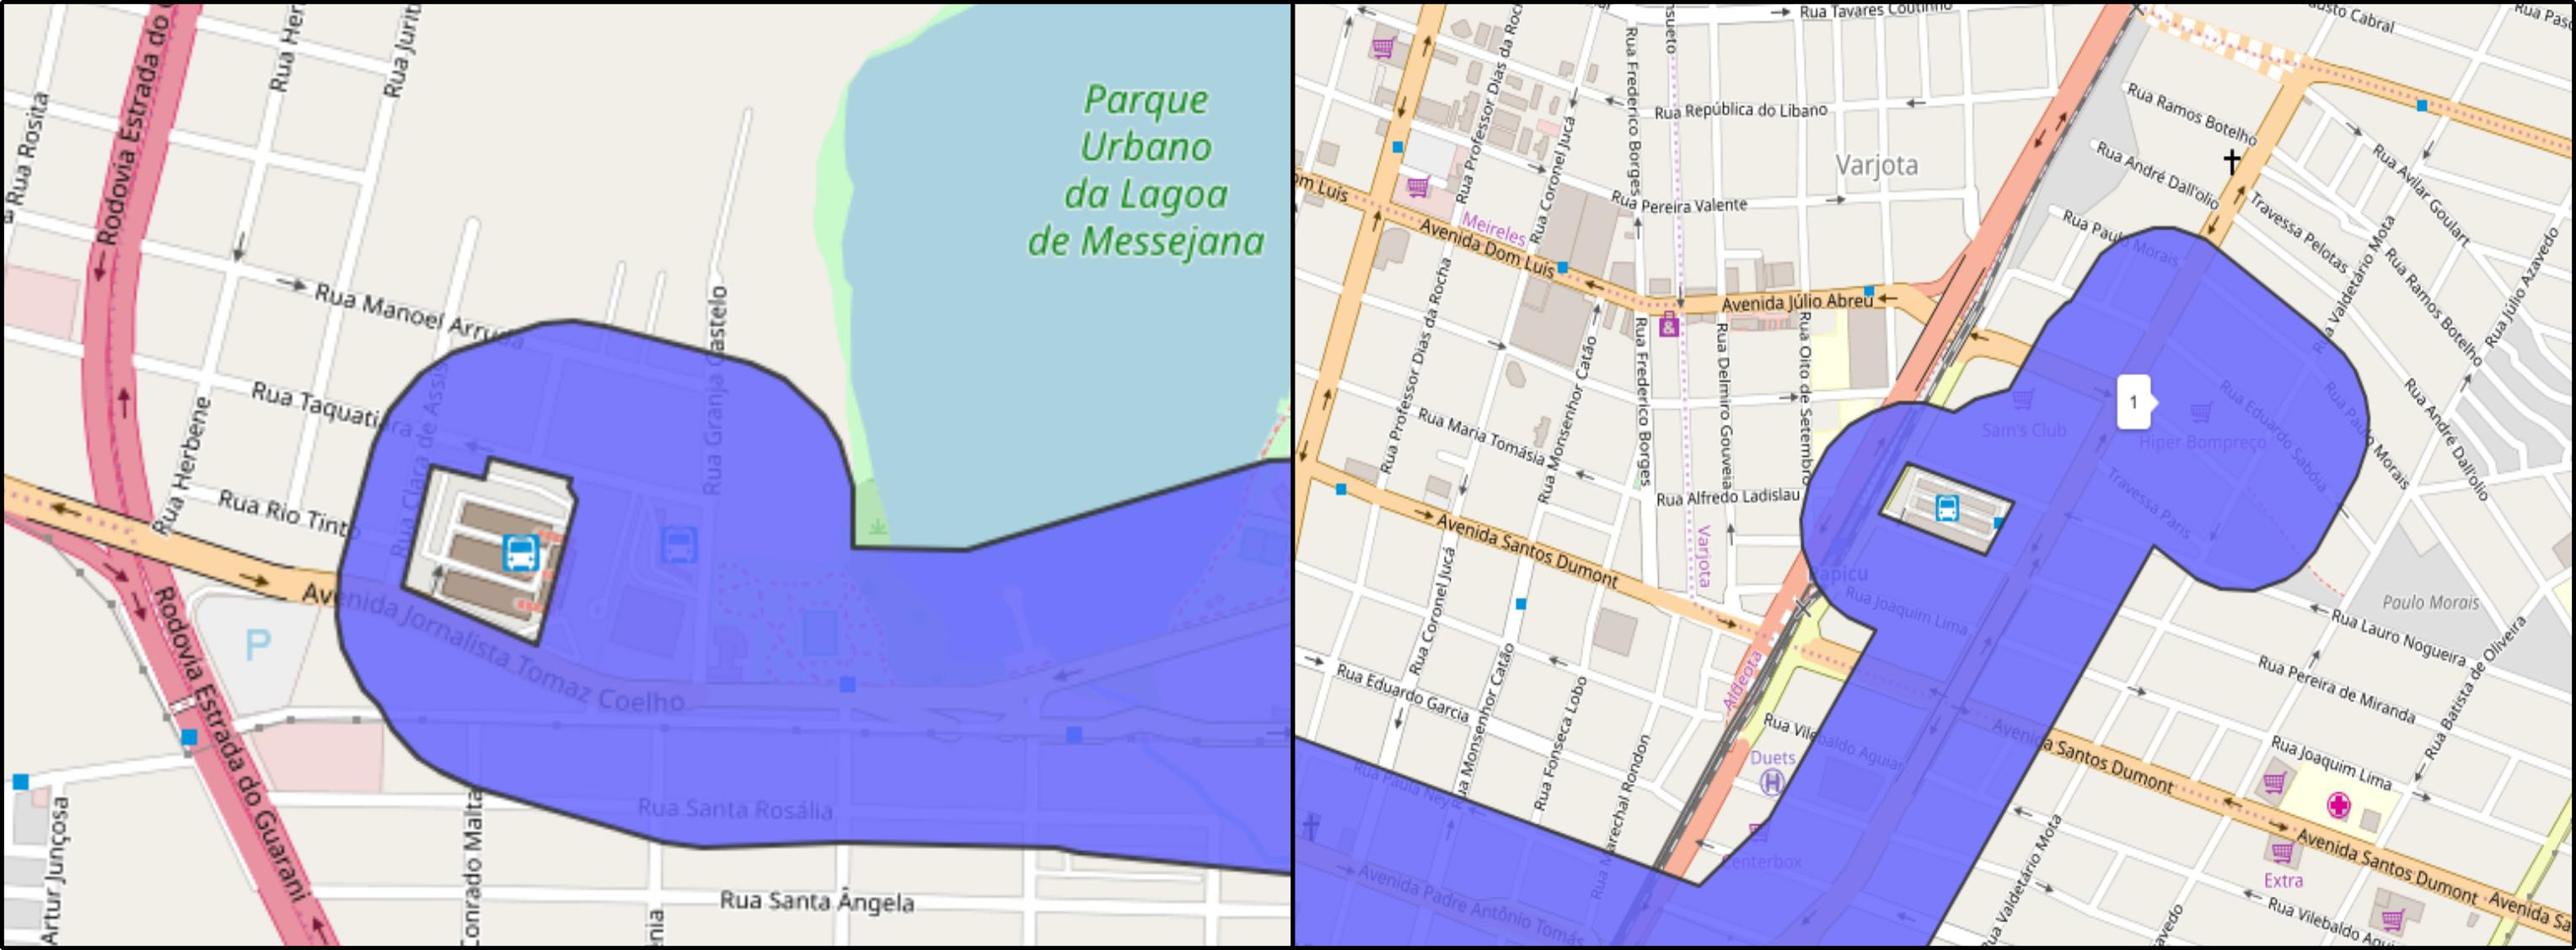
\includegraphics[width=16cm, keepaspectratio]{figure/3-buffer_terminais.jpg}}
  }{
  \Fonte{Elaborada pelo autor}
  }
  \end{figure}
  
  A base consolidada e integrada então é uma base filtrada, contando somente com os pontos que servem à linha, com a adição da coluna da \texttt{linha} e de uma outra coluna que informa se aquele ponto de GPS está na linha ou no começo/final dela.
  
  \hypertarget{aplicacao-do-metodo}{%
  \section{Aplicação do método}\label{aplicacao-do-metodo}}
  
  O método de consolidação foi aplicada para o dados do mês de setembro de 2019 para os dados de bilhetagem e GPS e para o GTFS da primeira semana de setembro. Esse mês foi escolhido porque representa uma época mais distante das férias de julho e já incorpora mudanças operacionais importantes como a validação sendo realizada pela parte da frente do veículo (entende-se que isso motiva o usuário a validar ao entrar no ônibus, porque ele tem menos espaço para aguardar).
  
  A Figura \ref{fig:qualidade_geo_bi} mostra a quantidade de validações realizadas por dia útil, com a distinção se elas foram georreferenciadas ou não. No total, 17\% das validações não tiveram sua localização estimada. Na comparação por dia, observa-se que a proporção de sucesso no georreferenciamento se mantém constante.
  
  \begin{figure}[!h]
  \captionsetup{width=16cm}
  \Caption{\label{fig:qualidade_geo_bi}Qualidade do georreferenciamento da bilhetagem}
  \centering
  \UFCfig{}{
  {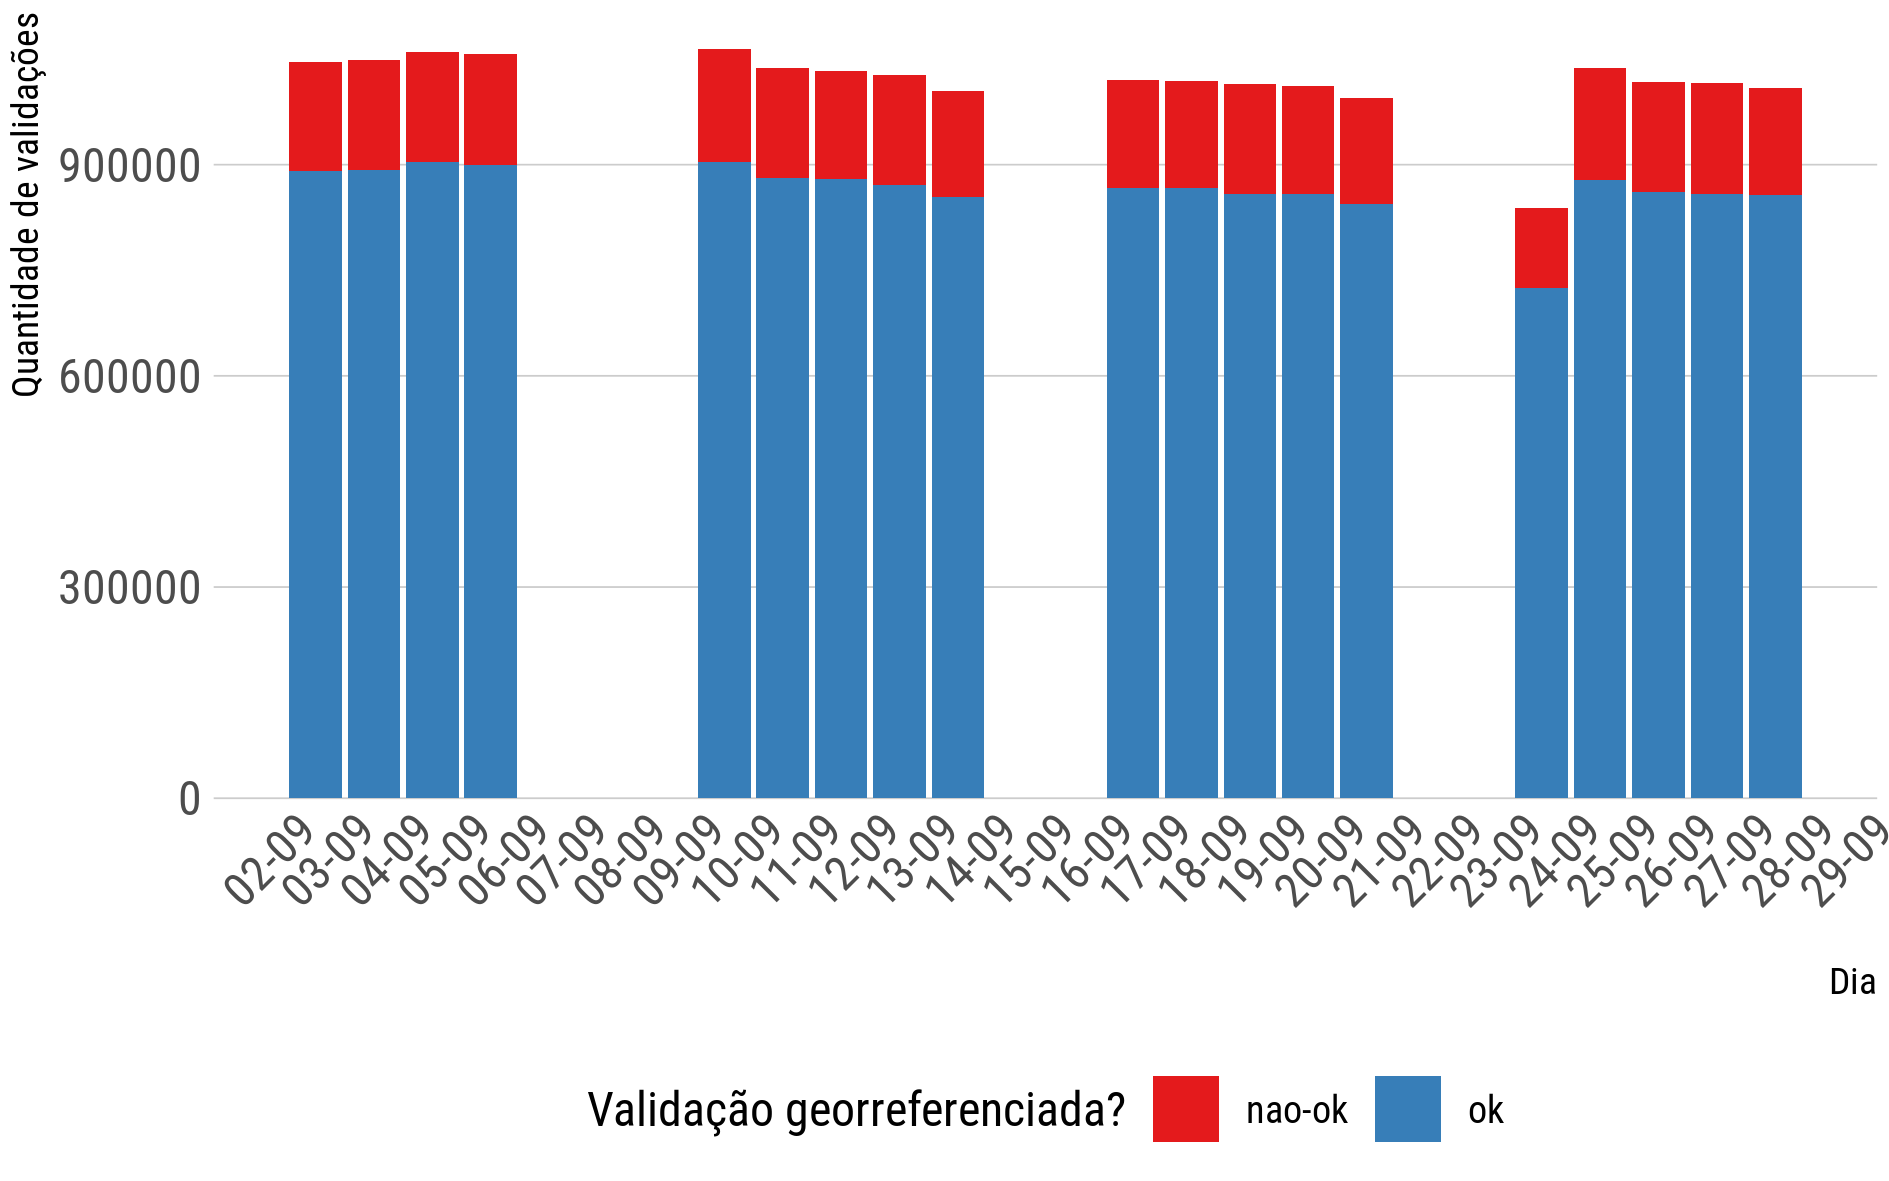
\includegraphics[width=16cm, keepaspectratio]{figure/3-qualidade_geo_bi.png}}
  }{
  \Fonte{Elaborada pelo autor}
  }
  \end{figure}
  
  O mesmo não acontece quando a comparação é feita por linhas. A Figura \ref{fig:qualidade_geo_bi_linhas} mostra linhas que não tiveram pelo 75\% das suas validações localizadas. Observa-se que grande parte delas são linhas do prefixo 7 (linhas complementares), que são de caráter alimentador (dos bairros para os terminais). Isso indica que esse sistema alimentador apresenta sérias falhas na integração das bases, comprometendo possíveis análises.
  
  \begin{figure}[!h]
  \captionsetup{width=16cm}
  \Caption{\label{fig:qualidade_geo_bi_linhas}Linhas com baixa qualidade de georreferenciamento}
  \centering
  \UFCfig{}{
  {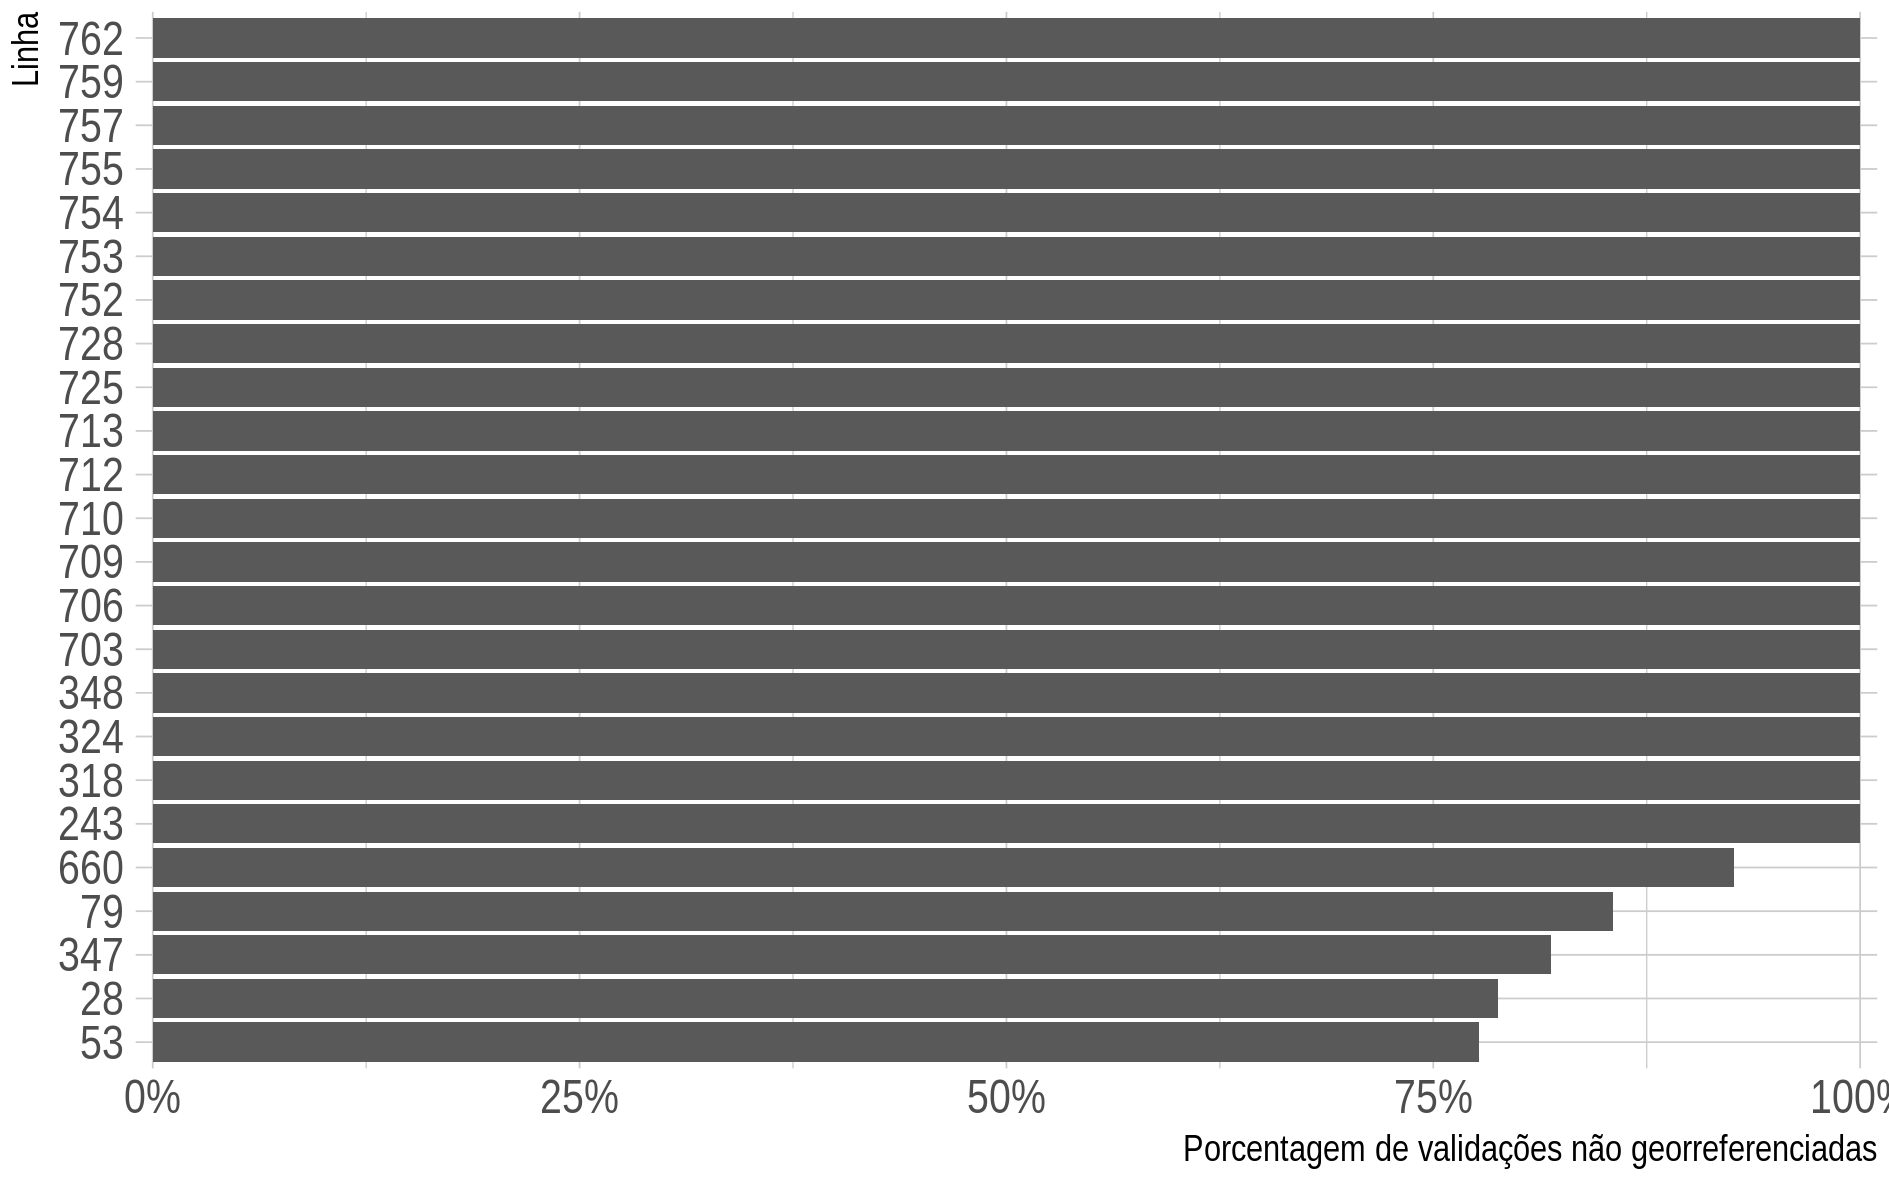
\includegraphics[width=16cm, keepaspectratio]{figure/3-qualidade_geo_bi_linhas.png}}
  }{
  \Fonte{Elaborada pelo autor}
  }
  \end{figure}
  
  A falta de integração das bases, consequentemente, também compromete a incorporação da informação da linha nos dados de GPS. A Figura \ref{fig:qualidade_geo_gps} mostra a quantidade de veículos que não tiveram a sua linha estimada proporcionalmente aos veículos totais, para os dias úteis de setembro de 2019. O perfil é semelhante ao encontrado na bilhetagem, onde aproximadamente 15\% da frota não teve sua linha identificada.
  
  \begin{figure}[!h]
  \captionsetup{width=16cm}
  \Caption{\label{fig:qualidade_geo_gps}Qualidade do georreferenciamento do GPS}
  \centering
  \UFCfig{}{
  {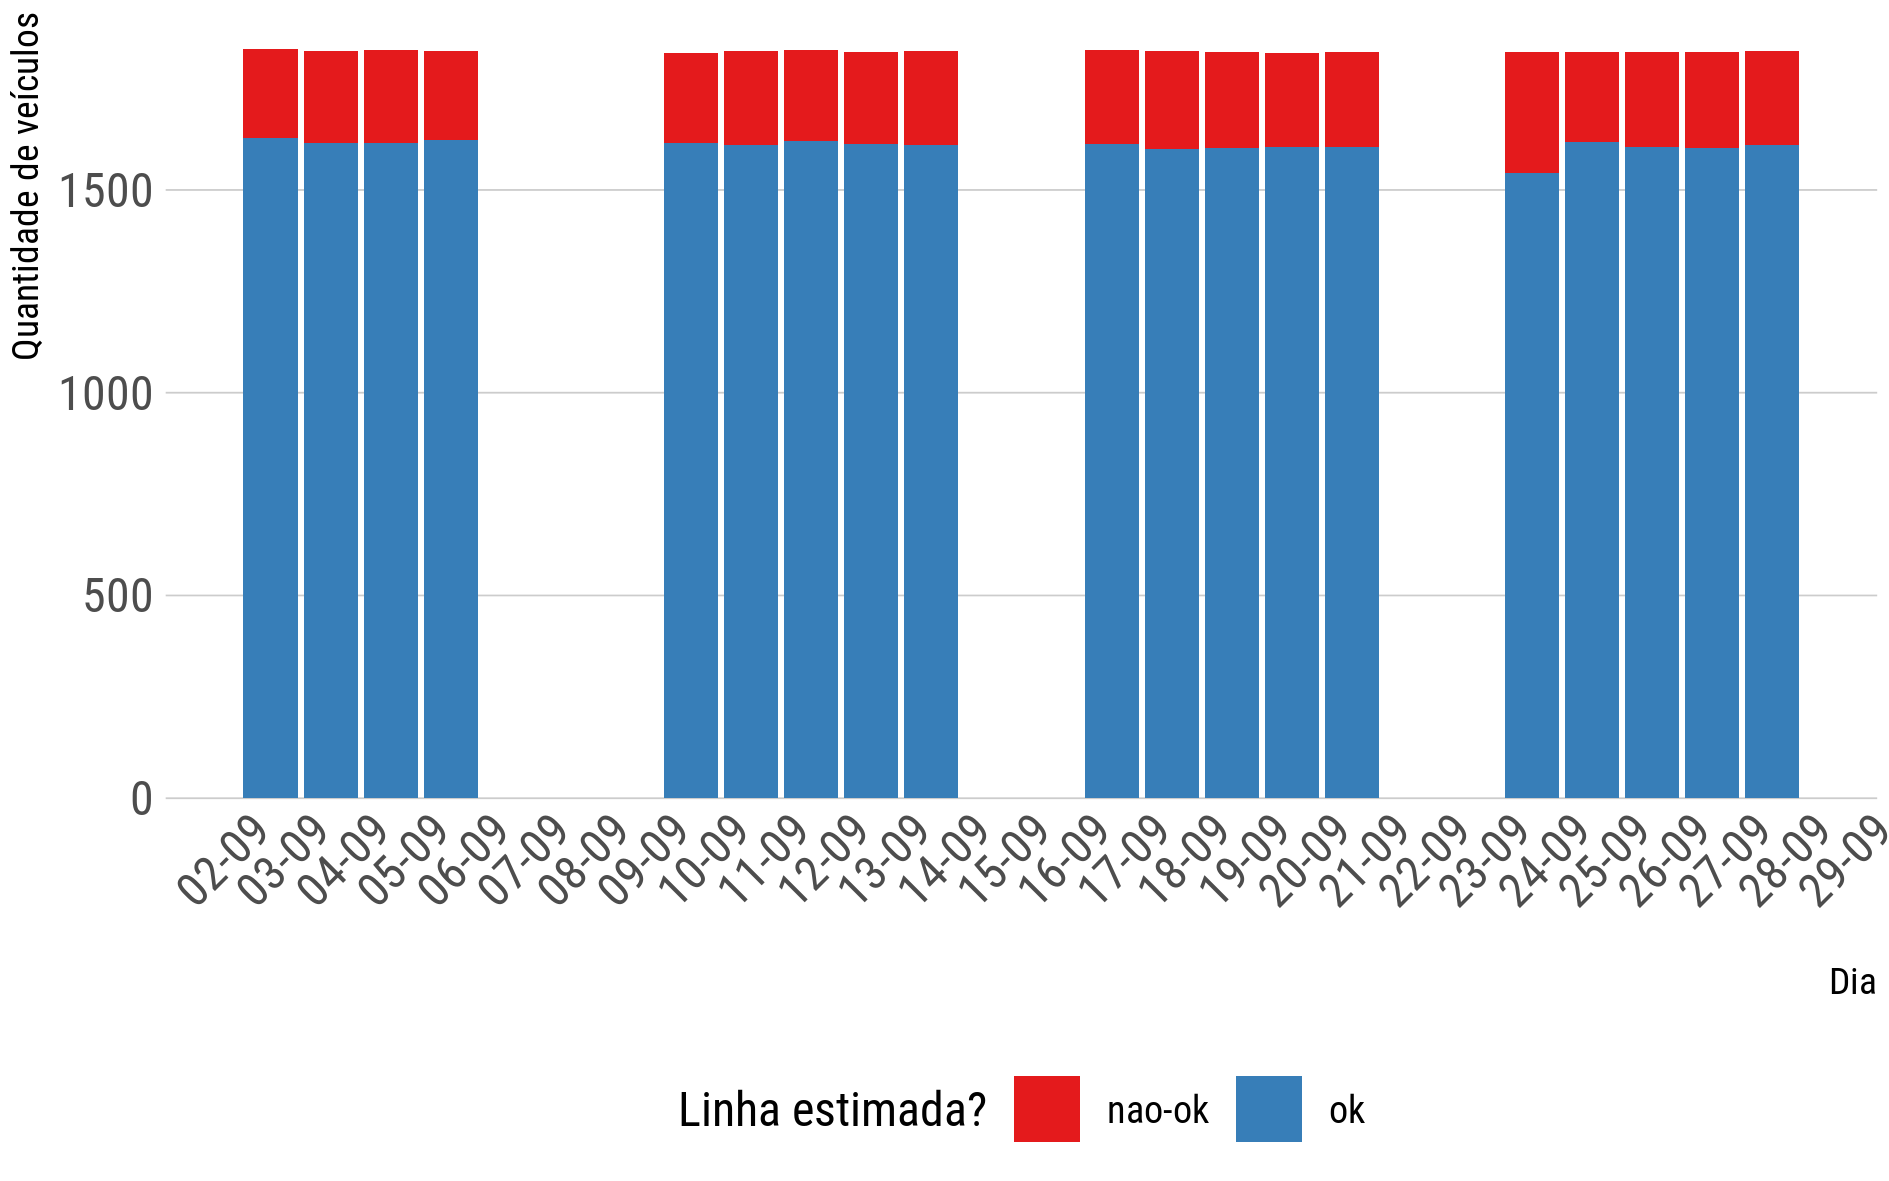
\includegraphics[width=16cm, keepaspectratio]{figure/3-qualidade_geo_gps.png}}
  }{
  \Fonte{Elaborada pelo autor}
  }
  \end{figure}
  
  Como determinado, a etapa do filtro espacial dos dados de GPS utiliza as informações do itinerário das linhas do arquivo de GTFS consolidado. Entretanto, o arquivo de GTFS não possui informações de algumas linhas importantes do SIT-FOR, e isso inclui todas as informações (itinerários, viagens realizadas, horários programados etc). Isso impõe outra limitação importante na integração dos dados. No total, 27 linhas estão faltando da base do GTFS. Para se ter uma dimensão, essas linhas recebem um total de 65 mil validações em um dia padrão, que representa cerca de 6\% do total de validações do sistema.
  
  \hypertarget{consideracoes-finais-1}{%
  \section{Considerações finais}\label{consideracoes-finais-1}}
  
  Essa etapa do trabalho fez uma introdução da cidade de Fortaleza e dos seus dados de transporte público. Foram estabelecidos métodos para o tratamento inicial e integração dos dados. A aplicação da metodologia focou numa análise da qualidade dos dados consolidados e integrados.
  
  A principal limitação se deu na etapa de integração. Primeiramente, as bases da bilhetagem e GPS apresentam a identificação do veículos com números diferentes. Um dicionário foi disponibilizado, mas ele não funciona perfeitamente, deixando alguns veículos de fora. Isso diminui a amostra disponível tanto para a bilhetagem como para o GPS, pois uma base depende da outra. Por fim, dados de GTFS não apresentavam informações de algumas linhas, o que diminuía ainda mais a amostra de análise.
  
  A consolidação e integração dos dados tem então como resultado dados de GPS, GTFS e bilhetagem que estão próximos para a próxima etapa de determinação do método. Os dados de GPS agora contém a linha, que torna a base a par com o que é encontrado com os dados utilizados na literatura. A base da bilhetagem tem a localização das validações, que a torna pronta para os métodos posteriores. Por fim, essa etapa também mostra a limitação da amostragem dos dados que vai guiar os processos daqui pra frente.
  
  \hypertarget{proposta-metodologica-para-analise-da-variabilidade-da-acessibilidade}{%
  \chapter{Proposta metodológica para análise da variabilidade da acessibilidade}\label{proposta-metodologica-para-analise-da-variabilidade-da-acessibilidade}}
  
  Esse capítulo busca estabelecer métodos para alcançar os três últimos objetivos do trabalho. Para isso, ele é dividido em duas etapas: a \textbf{integração entre GPS e GTFS} e a \textbf{análise comparativa da acessibilidade} (Figura \ref{fig:metodologia_geral}).
  
  \begin{figure}[!h]
  \captionsetup{width=16cm}
  \Caption{\label{fig:metodologia_geral}Metodologia geral do trabalho}
  \centering
  \UFCfig{}{
  {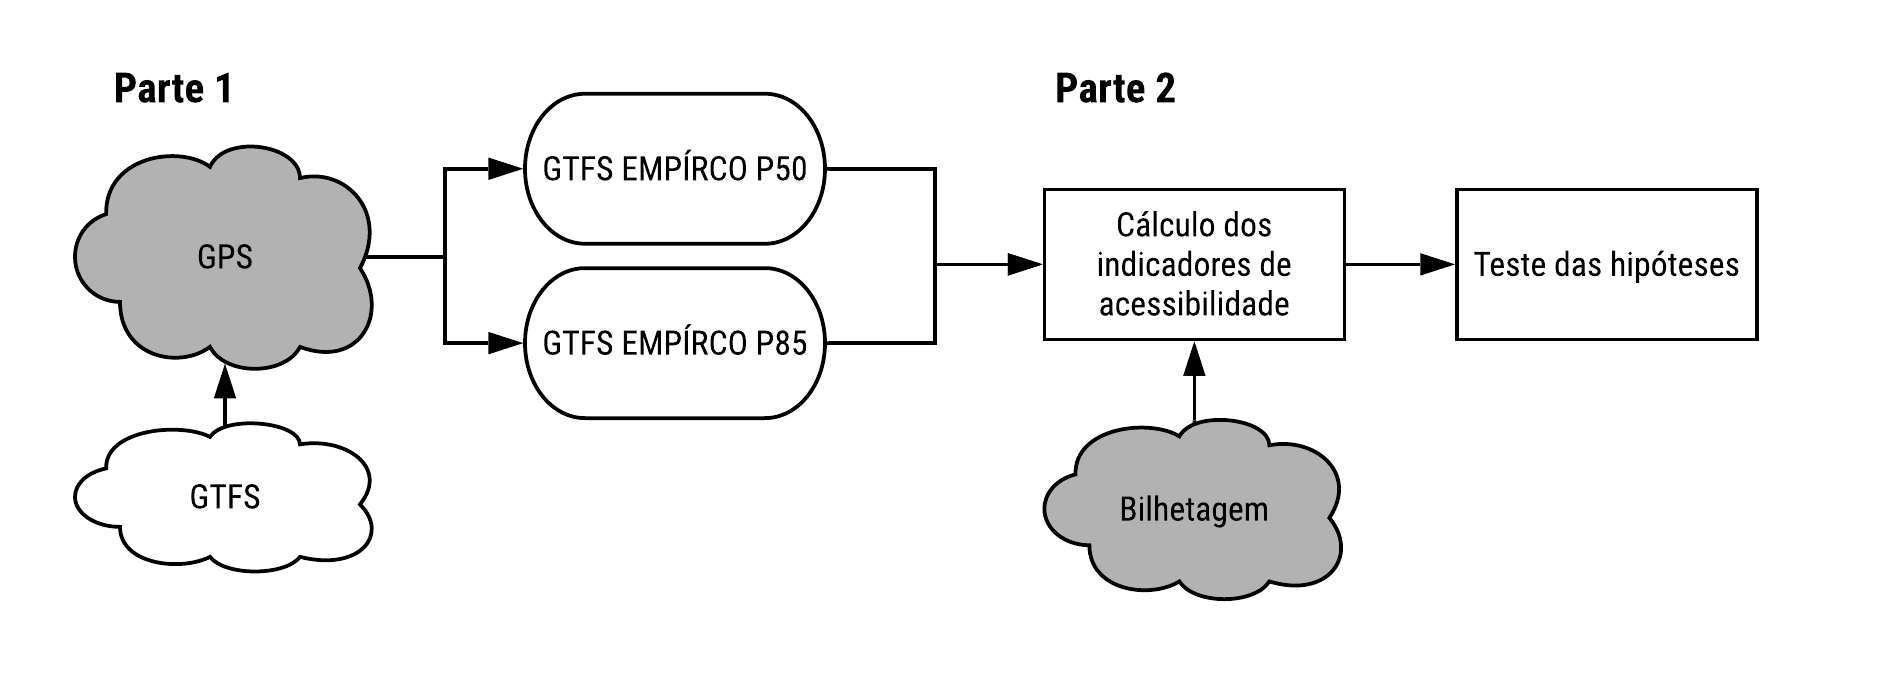
\includegraphics[width=16cm, keepaspectratio]{figure/4-metodologia_geral.png}}
  }{
  \Fonte{Elaborada pelo autor}
  }
  \end{figure}
  
  A primeira etapa busca suprir as lacunas de pesquisa identificadas no segundo objetivo do trabalho. Assim, é descrito o método que vai transformar dados consolidados de localização da frota em informações estruturadas de horários da oferta de transporte público análogo ao \emph{stop\_times.txt}. Esse método é desenvolvido tendo em vista as hipóteses apresentadas na introdução do trabalho.
  
  A segunda etapa apresenta os métodos utilizados para alcançar os três últimos objetivos específicos. Nela, é descrita a abordagem utilizada para calcular os indicadores com os dados estimados na etapa anterior, mostrando a importância da utilização de dados empíricos de tempos de viagem e do estudo de valores de dispersão do nível de serviço no sistema na variabilidade da acessibilidade. Assim, é descrita a abordagem utilizada para testar as três hipóteses determinadas.
  
  Por fim, as considerações finais apresentam limitações mais gerais do método e os principais desafios a serem enfrentados na sua aplicação.
  
  \hypertarget{reconstrucao-da-tabela-de-horarios-programados-do-gtfs-para-diferentes-cenarios}{%
  \section{Reconstrução da tabela de horários programados do GTFS para diferentes cenários}\label{reconstrucao-da-tabela-de-horarios-programados-do-gtfs-para-diferentes-cenarios}}
  
  Essa etapa utilizará os dados consolidados de GPS e de GTFS advindos do capítulo anterior. Esses dados apresentam dados de localização da frota para todos os dias úteis de setembro de 2018 (19 dias) e dados de GTFS da primeira semana do mesmo mês. A ETUFOR disponibiliza dados de GTFS para cada semana, onde pode haver alguma variabilidade em relação a horário ou rota das linhas. A Figura \ref{fig:metodologia_parte1} esquematiza o método.
  
  \begin{figure}[!h]
  \captionsetup{width=16cm}
  \Caption{\label{fig:metodologia_parte1}Metologia para reconstrução dos horários programados}
  \centering
  \UFCfig{}{
  {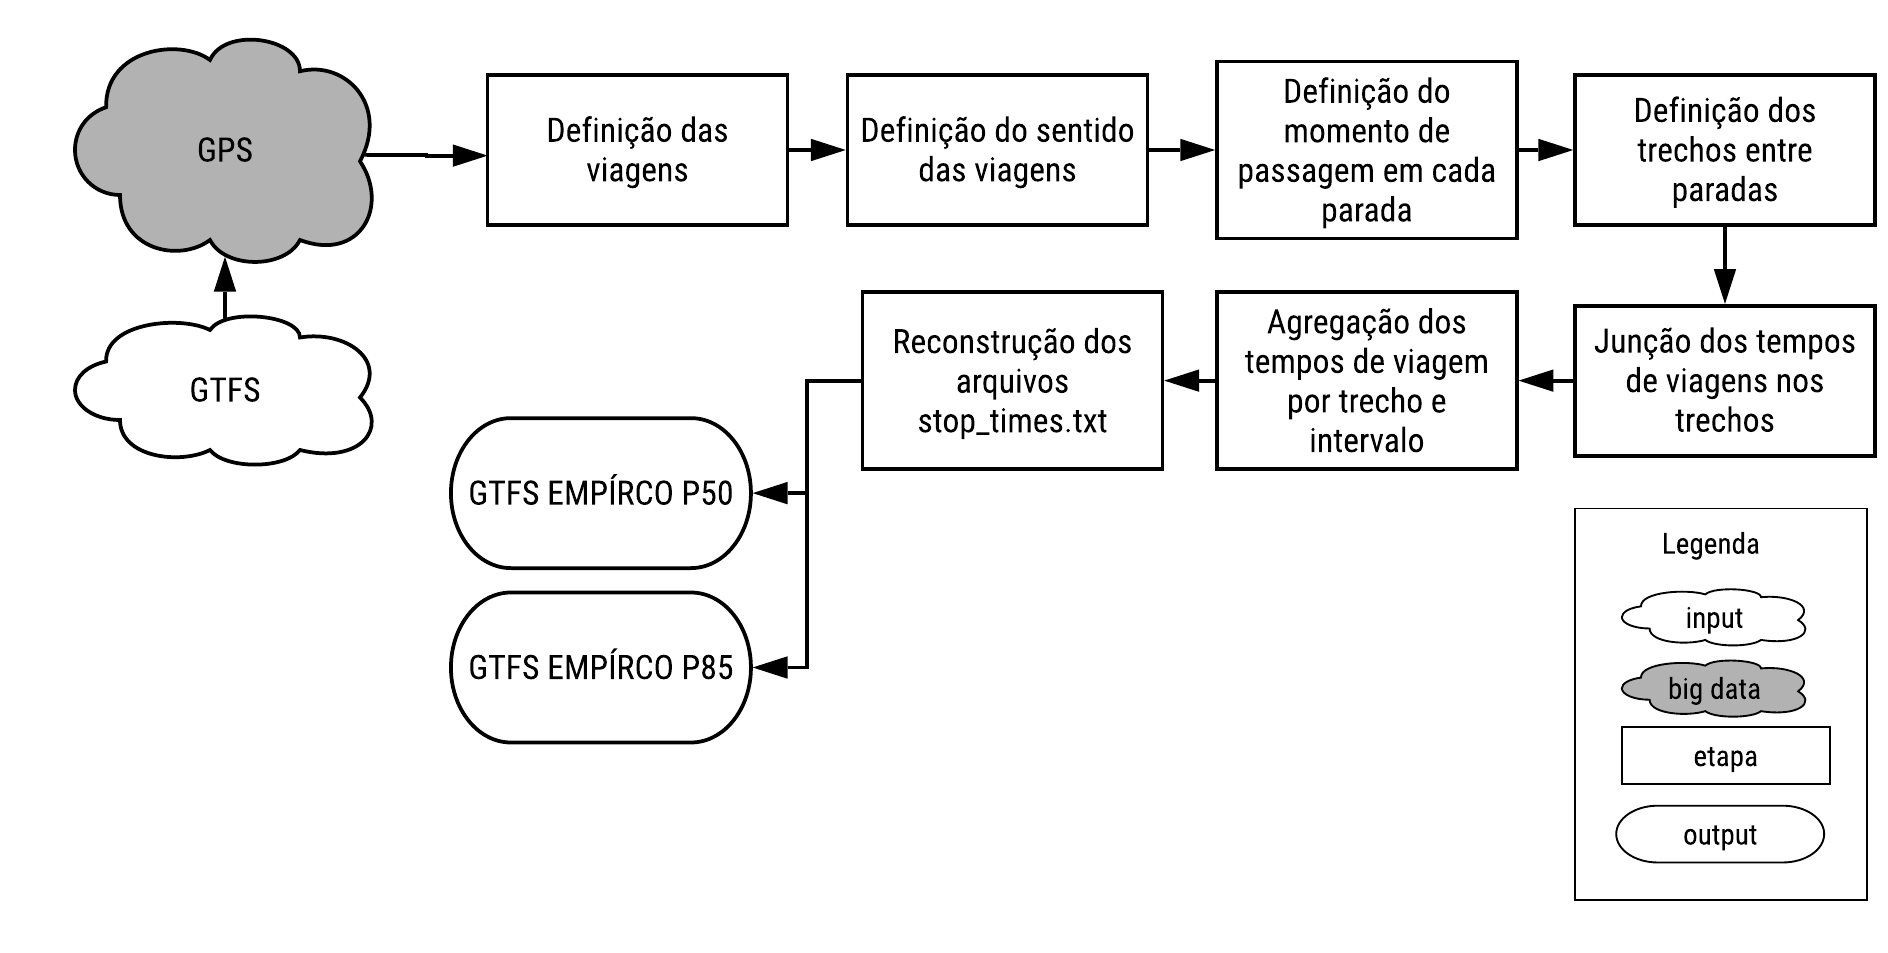
\includegraphics[width=16cm, keepaspectratio]{figure/4-metodologia_parte1.png}}
  }{
  \Fonte{Elaborada pelo autor}
  }
  \end{figure}
  
  \hypertarget{definicao-das-viagens}{%
  \subsection{Definição das viagens}\label{definicao-das-viagens}}
  
  Os dados consolidados de GPS receberam um filtro espacial onde somente os registros localizados dentro do itinerário da linha eram mantidos. O itinerário de cada linha foi dividido em três partes: uma parte representava o fim da linha, outra o começo e outra o trajeto comum. Quando a linha tinha como um extremo um terminal, o \emph{shape} do terminal era determinado como sendo a parte do começo/fim. Quando o extremo não era um ponto de terminal, foi estabelecido um buffer de 50 metros como sendo a área de início/fim. Assim, para cada registro de localização, é identificado a linha a que está servindo e se aquele registro é na rota ou no começo/fim da viagem.
  
  Com essa informação, o fim de uma viagem era determinado no primeiro registro de GPS dentro da área de começo/fim. O início da viagem seguinte, então, acontecia no último registro antes do veículo sair da área de início/fim de viagem. Esse método difere do de \citet{Arbex2016} e \citet{Rabay2017} porque permite considerar o tempo perdido de cada veículo com manobras/embarque/desembarque no fim/começo das suas viagens.
  
  A principal limitação acontecia quando um veículo porventura passava muito rápido pelo ponto de fim da viagem e acabava registrando só um ponto de GPS dentro da área de começo/fim, o que impossibilitava determinar o fim e o começo de acordo com o método. Quando isso acontecia, esses pontos eram duplicados, e o fim da viagem e começo da próxima eram assumidos como o mesmo ponto.
  
  \hypertarget{definicao-de-sentido-da-viagem}{%
  \subsection{Definição de sentido da viagem}\label{definicao-de-sentido-da-viagem}}
  
  Para definir o sentido da viagem (ida ou volta), o método estabelecido não foge do que é feito na literatura. Primeiramente, os registros de cada viagem são ordenados pelo momento do registro. Então, é feito um \emph{snap} de cada registro de GPS para a parada mais próxima de \textbf{ida} daquela linha, e essas paradas tinha uma identificação com a sequência que elas acontecem (\emph{stop\_sequence}). Por fim, era analisado: se os pontos de GPS daquela viagem estiverem indo no mesmo sentido da a sequência de paradas, a viagem estava indo no sentido da \textbf{ida}; senão, será viagem de \textbf{volta}.
  
  \hypertarget{momento-parada}{%
  \subsection{Definição do momento de passagem em cada parada e detecção de outliers}\label{momento-parada}}
  
  Por fim, para recompor a tabela de horário dos veículos, é necessário estimar o momento que cada veículo passou pelas paradas da sua correspondente linha e sentido. A abordagem aqui adotada leva em conta a distância acumulada percorrida pelos registros de GPS e a distância acumulada da posição das paradas, na linha em questão. A Figura \ref{fig:interpolacao} esquematiza o processo. Digamos que uma linha tenha o trajeto especificado abaixo. Primeiro, é feito o \emph{snap} do ponto de GPS para a linha. Segundo, é garantido que o primeiro ponto de GPS e a primeira parada estejam no mesmo ponto. A partir desse ponto, então, são calculadas as distâncias acumuadas na linha tanto dos pontos de GPS (em baixo) como das paradas (em cima). Do lado dos dados de GPS, cada ponto agora tem a distância acumulada na rede e o momento do registro de localização. É então feita uma interpolação linear que interpola a hora em cada distância acumulada da parada.
  
  \begin{figure}[!h]
  \captionsetup{width=16cm}
  \Caption{\label{fig:interpolacao}Interpolação do momento de passagem em cada parada}
  \centering
  \UFCfig{}{
  {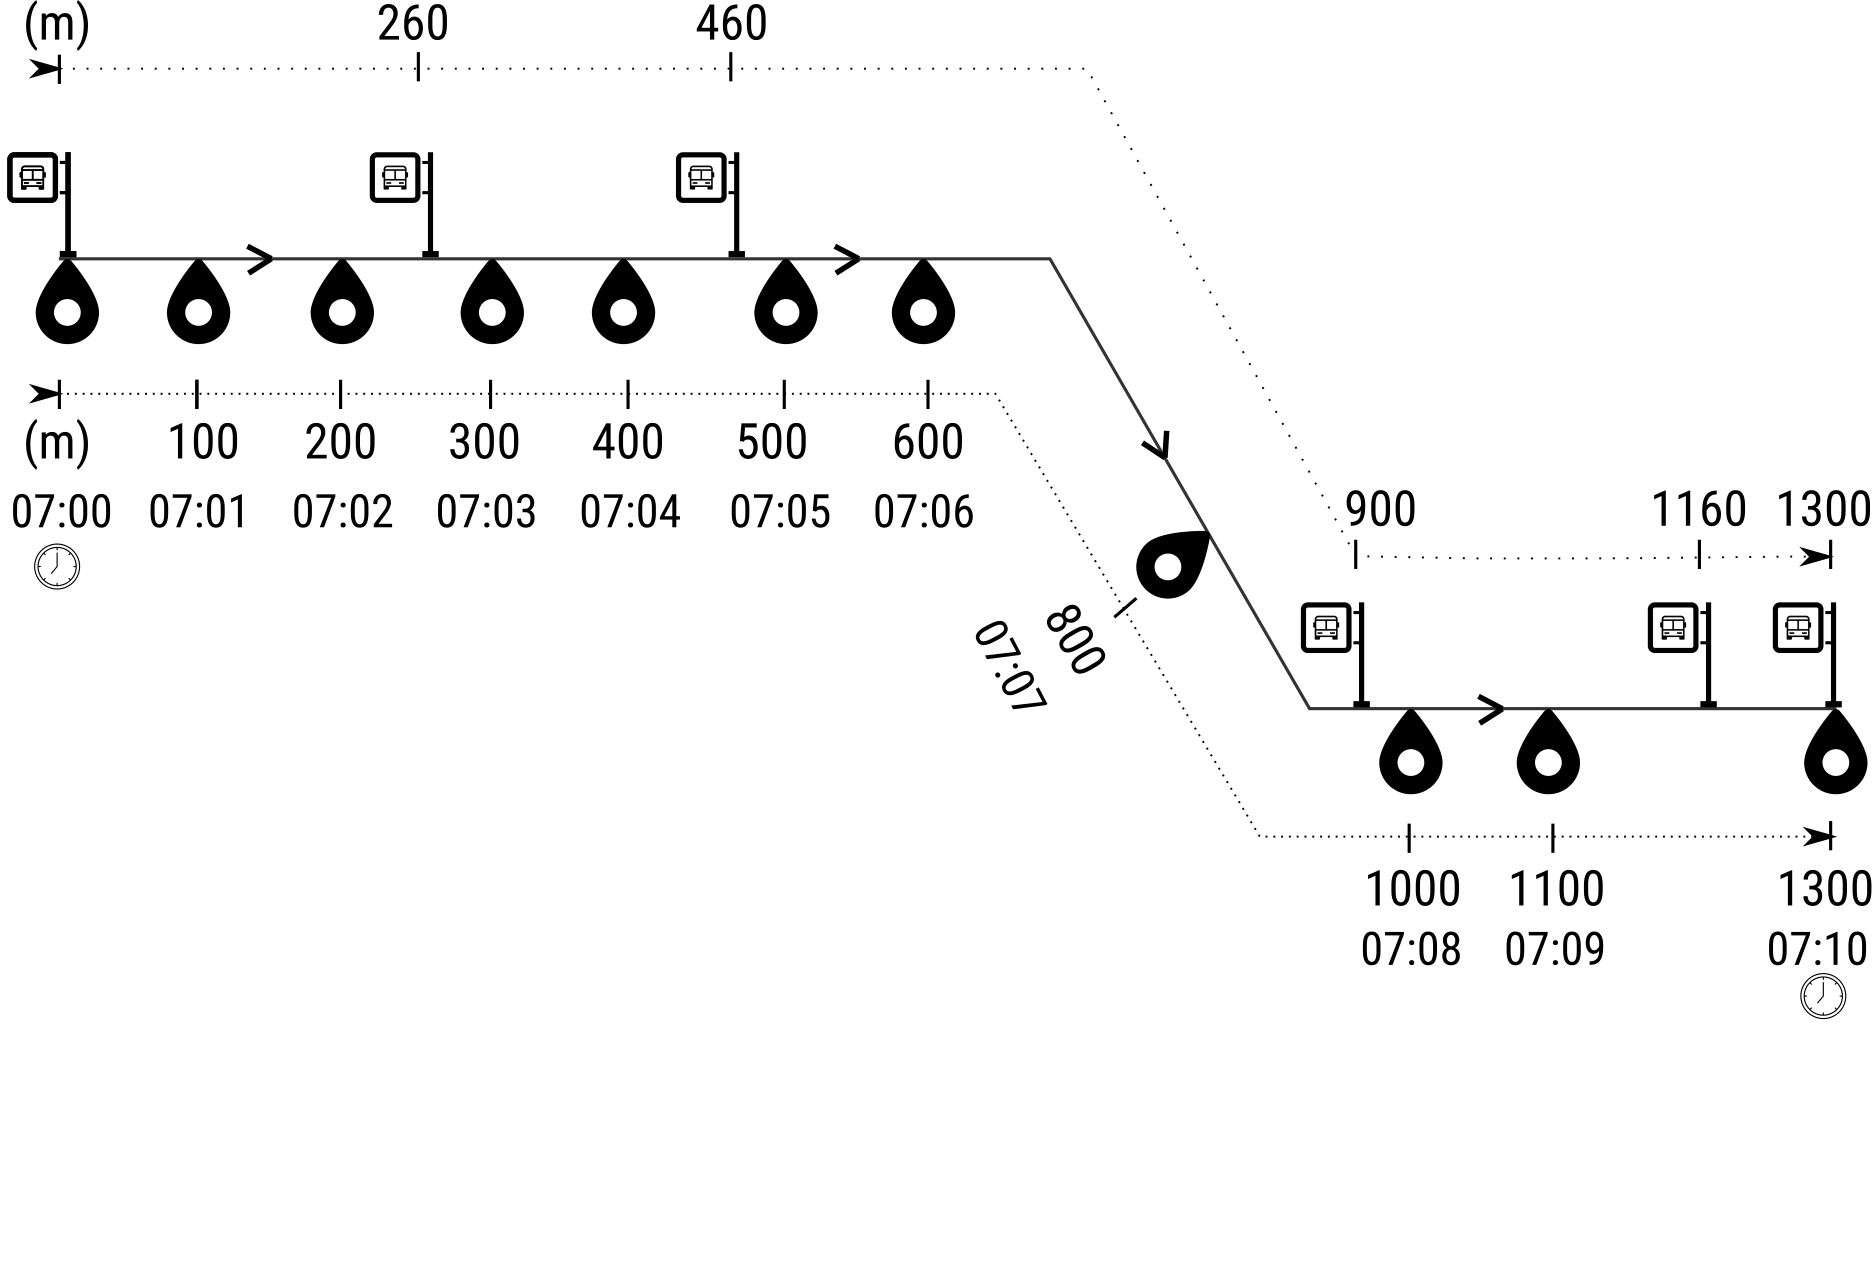
\includegraphics[width=16cm, keepaspectratio]{figure/4-interpolacao.png}}
  }{
  \Fonte{Elaborada pelo autor}
  }
  \end{figure}
  
  O processo de \emph{snap} do ponto de GPS para a linha pode ser problemático. Pontos de GPS podem ter variações na sua localização, o que muitas vezes pode fazer o ponto ser alocado para o trecho errado da linha. O caso mais clássico é quando uma linha, numa viagem do mesmo sentido, percorre trechos de uma mesma avenida, só que no sentido contrário. Isso, somado à imprecisão do GPS, leva certos pontos a serem alocados para o sentido errado da via naquele momento. Para contornar isso, pontos outliers são detectados e removidos.
  
  Acredita-se que essa metodologia representa uma avanço em relação às abordagens encontradas. \citet{Arbex2016}, contando com registros de GPS a cada 30 segundos, realiza um \emph{snap} para saber qual o registro está mais pŕoximo de cada parada, então assumindo esse registro como a hora de passagem caso ele esteja a no máximo 200 metros de distância da parada. \citet{Wessel2017} contam com uma amostragem maior de registros de GPS (10 segundos), então os autores fazem um \emph{buffer} de 20 metros em relação a cada parada e interceptam o registro que caia dentro daquela área. Os autores só aplicam técnicas de interpolação caso não seja possível estimar a hora de passagem em uma parada.
  
  Com os dados de GPS com informações consolidadas de linha, viagem, sentido e passagem em cada parada, e tendo em vista as limitações e hipóteses estabelecidas, é proposta uma agregação desses tempos de viagem por cada trecho.
  
  \hypertarget{definicao-dos-trechos-entre-paradas}{%
  \subsection{Definição dos trechos entre paradas}\label{definicao-dos-trechos-entre-paradas}}
  
  A proposta é fazer uma agregação espacial dos tempos de viagem coletados na etapa anterior, sendo isso feito utilizando o trecho que o veículo percorreu. Trecho é aqui definido como qualquer segmento entre paradas seguidas em que algum veículo de algum linha esteja programado para trafegar no SIT-FOR. A criação dos trechos começa na coleta, a partir dos dados de horários programados \emph{stop\_times.txt}, dos trechos em que todos os veículo do sistema esteja programado para rodar. Essa informação mostra todos os trechos possíveis e os pontos de começo e fim de cada um deles. Para recompor mais detalhadamente os trechos, é feito o uso do arquivo \emph{shapes.txt}, que apresenta pontos de cada uma das linhas com uma maior resolução espacial. Por fim, o arquivo final apresenta todos os trechos possíveis com a informação do comprimento total e da geolocalização na forma de uma \emph{linestring} (Figura \ref{fig:trecho_paradas}).
  
  \begin{figure}[!h]
  \captionsetup{width=16cm}
  \Caption{\label{fig:trecho_paradas}Criação dos trechos entre paradas}
  \centering
  \UFCfig{}{
  {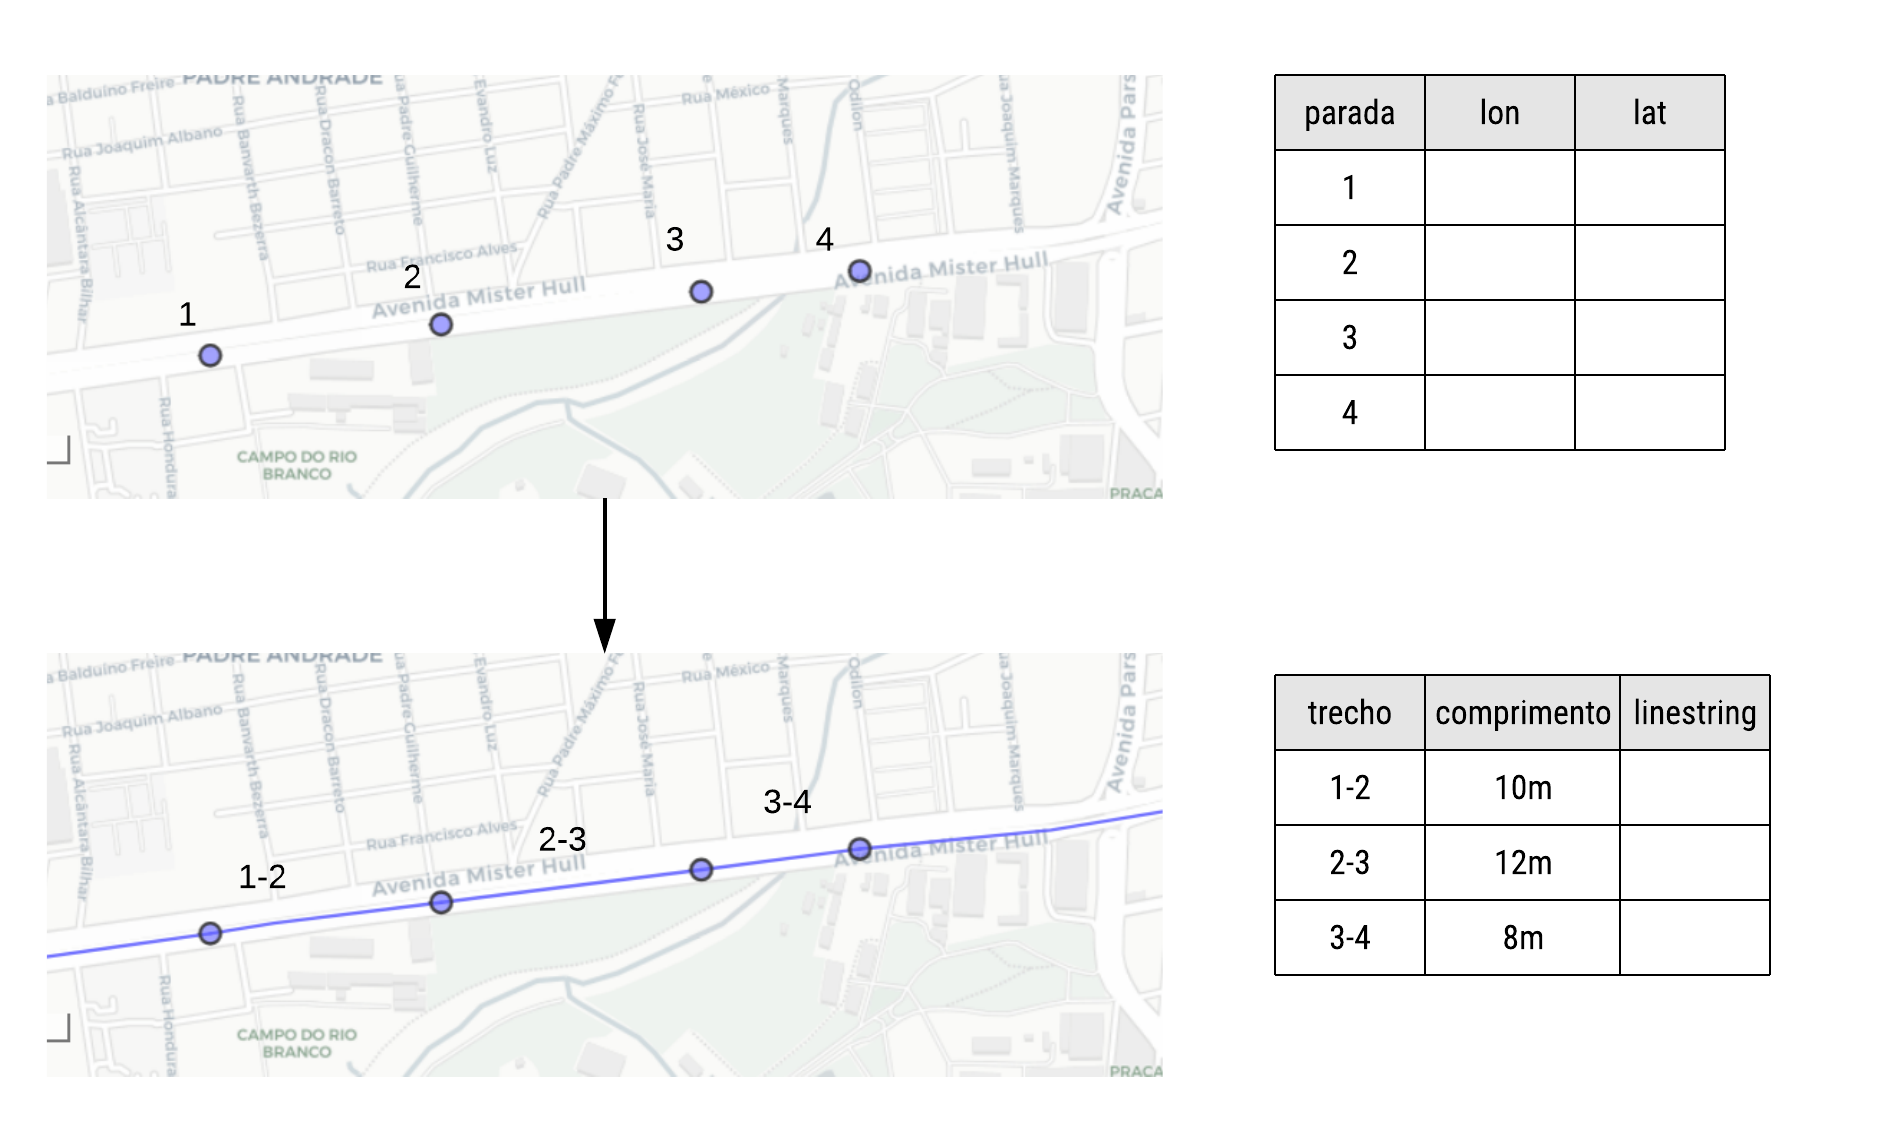
\includegraphics[width=16cm, keepaspectratio]{figure/4-trecho_entre_paradas.png}}
  }{
  \Fonte{Elaborada pelo autor}
  }
  \end{figure}
  
  \hypertarget{juncao-dos-dados-de-gps-para-os-trechos-entre-paradas}{%
  \subsection{Junção dos dados de GPS para os trechos entre paradas}\label{juncao-dos-dados-de-gps-para-os-trechos-entre-paradas}}
  
  Os dados de GPS resultantes da seção \ref{momento-parada} apresentam uma estrutura semelhante aos dados de viagens agendadas do GTFS, com o registro da hora em que cada veículo passou em cada parada daquela linha. Buscando saber o tempo de viagem de cada trecho de viagem realizado por cada veículo, é feita a junção dos dados de GPS para os trechos de paradas. O primeiro passo transforma os dados de GPS de uma estrutura de paradas para uma estrutura de trechos (Figura \ref{fig:gps_para_trechos}, Passo 1). O segundo passo, por fim, trás as informações disponibilizadas na etapa anterior de comprimento e localização do trecho (Figura \ref{fig:gps_para_trechos}, Passo 2). Esse tipo de informação não é utilizada na recomposição dos horários dos veículos, mas é importante para testar a qualidade da amostra futuramente. A base resultante apresenta as informações do tempo de viagem de cada veículo de cada linha a cada trecho percorrido, com a consequente informação do comprimento do trecho.
  
  \begin{figure}[!h]
  \captionsetup{width=16cm}
  \Caption{\label{fig:gps_para_trechos}GPS paradas para trechos}
  \centering
  \UFCfig{}{
  {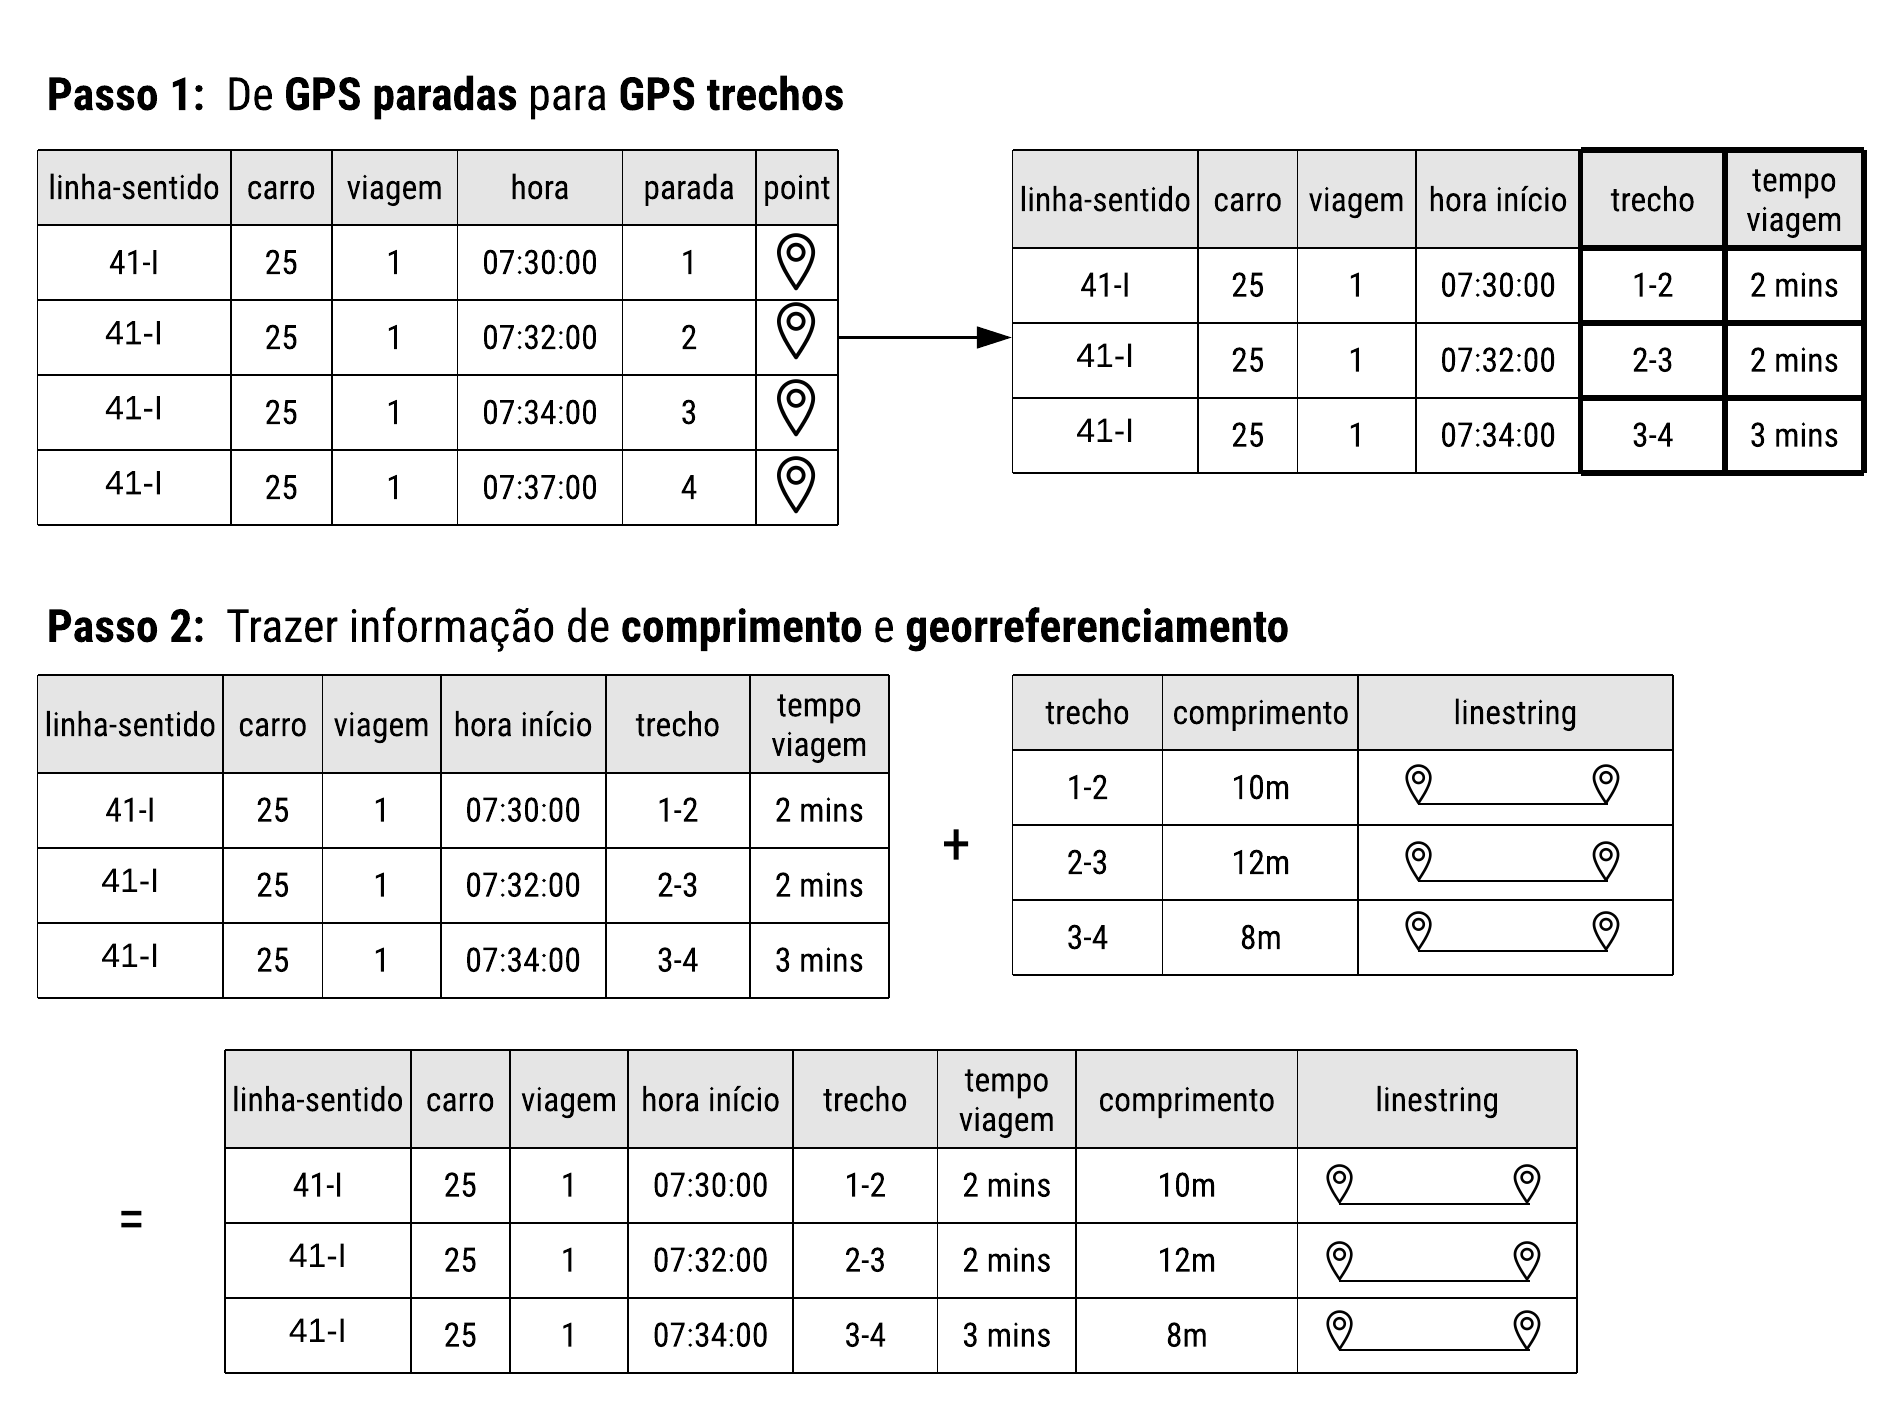
\includegraphics[width=16cm, keepaspectratio]{figure/4-gps_para_trechos.png}}
  }{
  \Fonte{Elaborada pelo autor}
  }
  \end{figure}
  
  \hypertarget{agrupamento-dos-tempos-de-viagem-nos-trechos-e-intervalo-de-15-minutos}{%
  \subsection{Agrupamento dos tempos de viagem nos trechos e intervalo de 15 minutos}\label{agrupamento-dos-tempos-de-viagem-nos-trechos-e-intervalo-de-15-minutos}}
  
  Ao contrário dos trabalhos já realizados que utilizaram dados de GPS para a reconstrução do arquivo de GTFS \citep{Wessel2017}, aqui é adotada uma metodologia de agregar os tempos de viagens nos trechos estimados a cada 15 minutos. Isso foi feito por duas razões: 1) não foi possível estimar os tempos de viagens entre as paradas de todos os veículos do SIT-FOR, então não é possível recompor a oferta completa do sistema só pelos dados de GPS e 2) a agregação permite estimar para cada trecho tempos de viagem medianos e de 85º percentil, o que possibilita reconstruir dois arquivos \emph{stop\_times} para estudar a variabilidade da acessibilidade em função da dispersão do tempo de viagem nos trechos, verificando a segunda hipótese.
  
  A base final da etapa anterior tem, para todos os dias úteis do mês de setembro/2018, informações de tempo de viagens em cada um dos trechos que foram captados a partir das informações do GPS, com o registro do momento exato em que cada veículo passou pelo trecho que era previsto. Buscando agrupar as informações para cada trecho de parada do sistema, primeiramente o momento de passagem de cada veículo por cada trecho é aproximado para o intervalo de 15 minutos mais próximo (etapa 1 da Figura \ref{fig:agregar_tempos_trechos}). Em seguida, para todas as viagens realizadas por todas as linhas, é feito um agrupamento desses tempos de viagem por trecho e intervalo para duas medidas: a mediana (P50) e o 85º percentil (P85) da distribuição do tempo de viagem (etapa 2 da Figura \ref{fig:agregar_tempos_trechos}). Assim, é criada uma base de dados com duas colunas de tempo de viagem: uma representando o tempo de viagem em todos os trechos (em cada intervalo de 15 minutos) para uma situação mediana, e outra representando uma medida de dispersão (no que diz respeito ao tempo de viagem) do sistema.
  
  \begin{figure}[!h]
  \captionsetup{width=16cm}
  \Caption{\label{fig:agregar_tempos_trechos}Agregação dos tempos de viagens nos trechos}
  \centering
  \UFCfig{}{
  {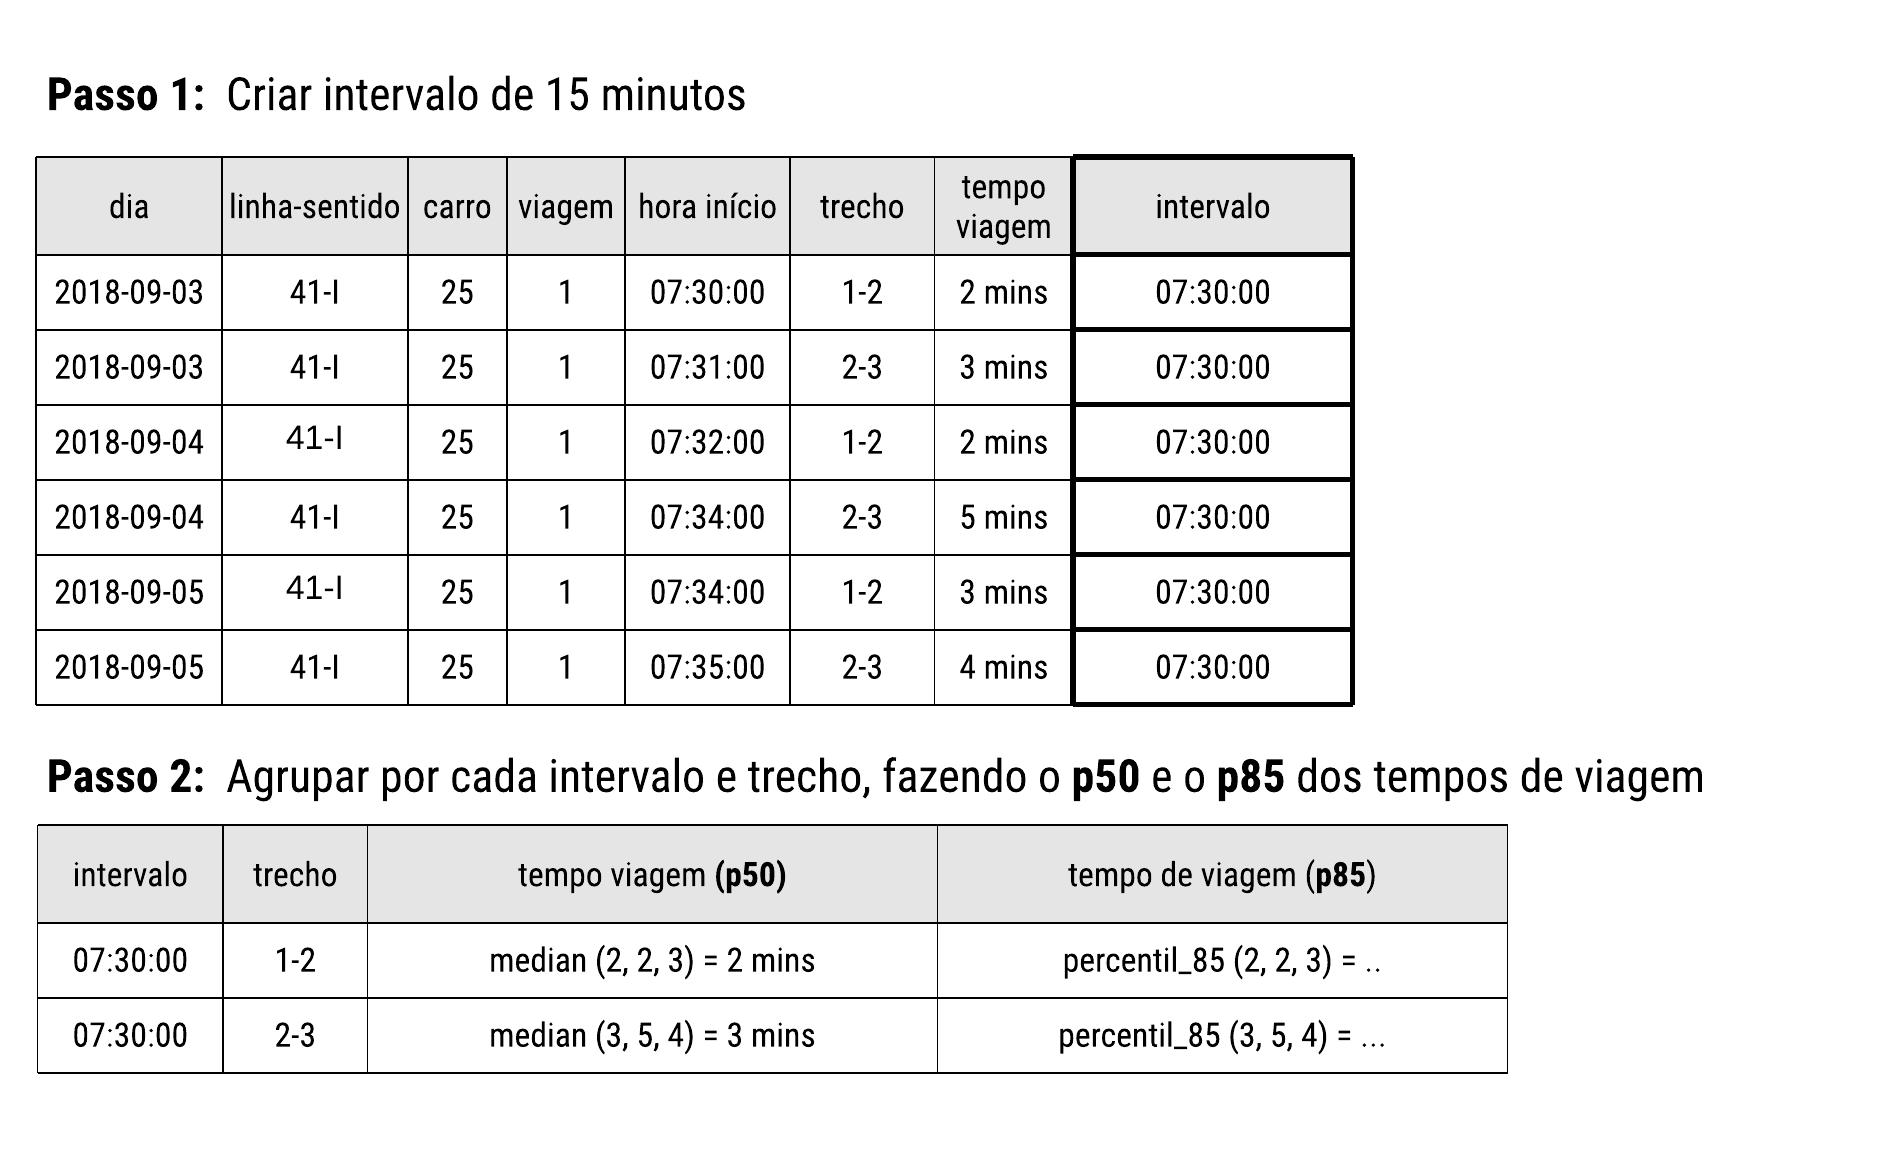
\includegraphics[width=16cm, keepaspectratio]{figure/4-agregar_tempos_trechos.png}}
  }{
  \Fonte{Elaborada pelo autor}
  }
  \end{figure}
  
  O tamanho da amostra de tempo de viagem de cada trecho vai depender da quantidade de linhas que passam por ali (trechos em avenidas troncais tendem a ter uma amostra bem maior do que trechos em ruas locais) e do intervalo em questão (horário de pico tende a ter uma frequência maior de ônibus). Dessa forma, os percentis 50 e 85 tendem a ser mais confiáveis em trechos com uma amostra maior, e é importante que assim o seja: esses trechos pertencem a avenidas que apresentam níveis maiores de congestionamento. Para trechos mais locais, por conta da menor amostra, os percentis tendem a ser menos significativos, mas a própria variação do tempo de viagem tende a ser menor, então isso tende a ser suavizado.
  
  Observações de tempo de viagem de um trecho que ficaram de fora do valor de 1.5 * IQR (\emph{Inter Quartile Range}, ou o intervalo entre quartis 0.25 e 0.75) foram excluídas, entendendo que poderiam representar um estado atípico do sistema, como acidentes, chuva, problemas mecânicos do veículo etc. Para garantir que o trecho tenha uma amostra de tempo de viagem significativa, trechos que tiveram menos que 10 observações são excluídos. Além disso, trechos com coeficiente de variação (divisão da média pelo desvio padrão) do tempo de viagem maior que 100\% também são excluídos.
  
  É entendido que dentro de um mesmo intervalo de 15 minutos pode acontecer uma flutuação natural do tempo de viagem nos trechos do sistema. Por exemplo, é esperado que em certo trechos o tempo de viagem de um veículo que passa às 06:23 e outro que passa às 06:37 tenha uma variação natural, e estes tempos de viagem são agregados para o mesmo intervalo de 06:30. A utilização do percentil 85 busca então identificar tempos de viagem que ao mesmo tempo não sejam tão extremos (como no caso do uso de percentil acima do 90) e que não façam parte da variação natural do serviço dentro do intervalo. Também é importante frisar que a agregação de dias úteis de um mês de dados assume que tempos de viagens tem pouca variação entre dias da semana ou entre semanas desse mês específico.
  
  A utilização do percentil 85 para os tempos de viagem também vai de encontro à distribuição da variável. Apesar de não ser assumido aqui que os tempos de viagem em cada trecho têm uma distribuição normal, o percentil 85 é utilizado porque aproximadamente representa o valor de 1 desvio padrão em relação à média da distribuição.
  
  A abordagem de agregar os tempos de viagem nos trechos para dois percentis é diferente do que foi feito nos trabalhos de \citet{Wessel2017} e \citet{Arbex2016a}. No primeiro, a abordagem foi bem diferente: os autores calcularam o tempo de viagem para dois dias e os usaram como eles acontecem para reconstruir o \emph{stop\_times} e para calcular o indicador de acessibilidade, então fazendo a média dos dois valores do indicador calculado (amostra n = 2). Essa abordagem, portanto, só leva em consideração o estado do sistema em especificamente dois dias. No último, é mencionado que foram coletados 20 dias de tempos de viagem, porém não é mencionado como essa amostra foi utilizada para recompor um arquivo único \emph{stop\_times}.
  
  \hypertarget{reconstrucao-dos-arquivos-stop_times-do-gtfs}{%
  \subsection{\texorpdfstring{Reconstrução dos arquivos \emph{stop\_times} do GTFS}{Reconstrução dos arquivos stop\_times do GTFS}}\label{reconstrucao-dos-arquivos-stop_times-do-gtfs}}
  
  O método, então, resumidamente busca substituir os tempos de viagem entre paradas que foram programados com tempos de viagem empíricos, para intervalos de 15 minutos iguais, depois somando-os cumulativamente. Essa abordagem traz alguns desafios. Uma tabela de horários de um sistema de transporte público de média-alta complexidade é mais que somente a soma dos tempos que os veículos percorreram ao longo da sua rota. Então, foi necessário investigar diversos pormenores que estavam presentes na tabela. Após inspeção visual e consulta com gestores do sistema, foram levantadas e confirmadas algumas hipóteses:
  
  \begin{itemize}
  \tightlist
  \item
    Cada operador de um veículo (motorista e/ou cobrador) tem direito a um descanso entre 30 e 59 minutos a cada 2 horas de trabalho, em média. Esses descansos estão previstos na tabela de horários;
  \item
    Outras pausas mais longas, entre 1h e 2h, também estão previstas;
  \item
    Veículos que estão adiantados em relação ao programado fazem pausas mais longas e começam a viagem seguinte no horário programado.
  \end{itemize}
  
  Tendo essas informações em mente, foi necessário estabelecer duas premissas para a reconstrução: 1) o horário da primeira partida de cada veículo é correto e 2) a oferta (quantidade de veículo rodantes) é correta. De acordo com os gestores do sistema e com os dados que foram apresentados, essas premissas são factíveis, principalmente porque o repasse dos recursos para as empresas operadoras do sistema depende da pontualidade da primeira viagem e da quilometragem rodada (em relação à prevista) de cada linha.
  
  A Figura \ref{fig:reconstrucao_gtfs} esquematiza o método desenvolvido para reconstruir o arquivo com os horários programados. A primeira tabela à esquerda apresenta a tabela dos horários agendados de um carro de uma linha 41, nas primeiras 4 paradas. Na direta, tem-se a tabela agregada do GPS com o tempo de viagem mediano (só para demonstração) de todos os carros que passaram em cada um dos trechos determinados, no intervalo de 07:00:00 (valores são agregado para o intervalo de 15 minutos mais próximo, como explicado na metodologia). Confirmado que os intervalos da hora programada e do GPS são condizentes, é assumido então que o horário da primeira partida do carro é o horário correto (em verde). Dessa forma, para cada trecho de viagem correspondente, é feita a soma acumulada dos tempos de viagens a partir do primeiro horário, resultando na tabela (na parte inferior) com o horário acumulado corrigido.
  
  \begin{figure}[!h]
  \captionsetup{width=16cm}
  \Caption{\label{fig:reconstrucao_gtfs}Reconstrução do arquivo stoptimes}
  \centering
  \UFCfig{}{
  {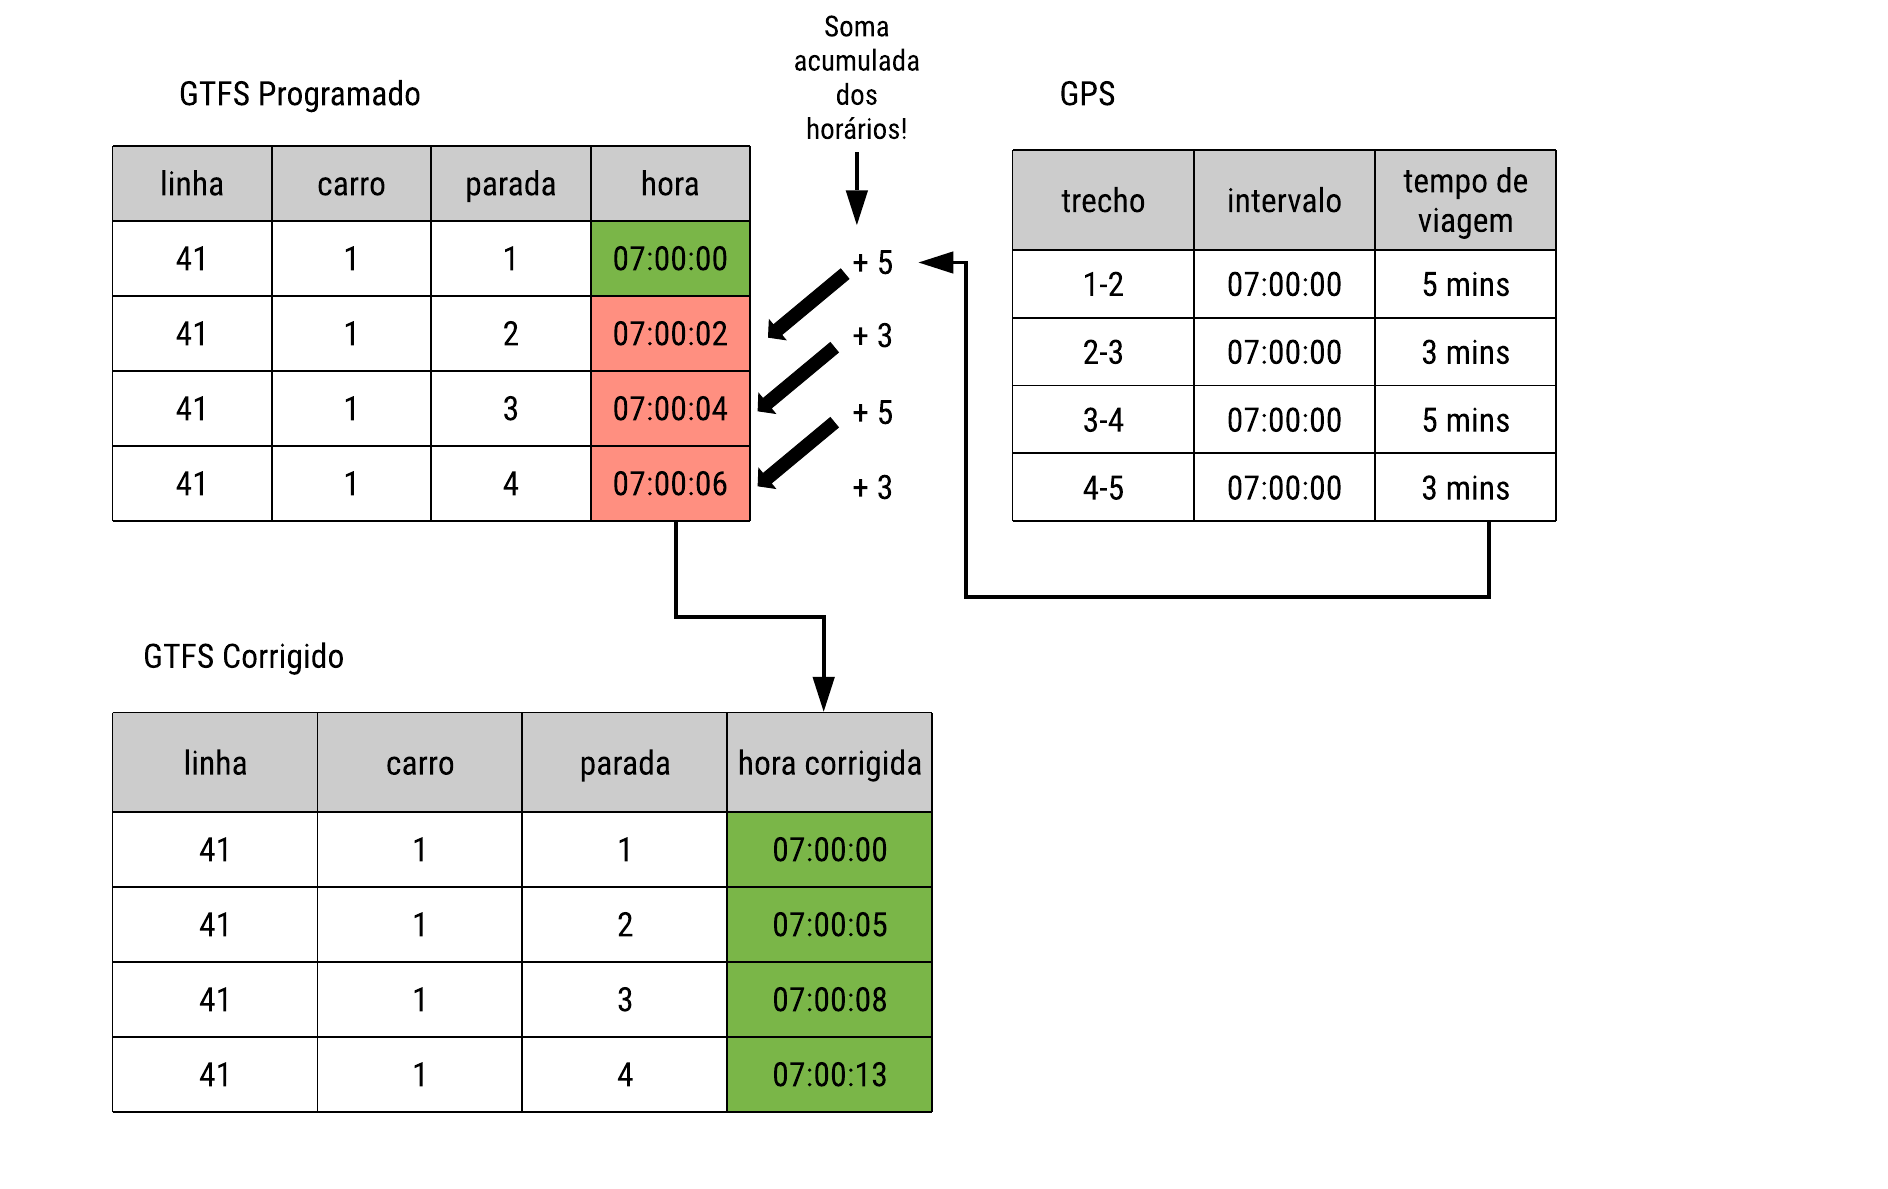
\includegraphics[width=16cm, keepaspectratio]{figure/4-metodologia_reconstrucao_gtfs.png}}
  }{
  \Fonte{Elaborada pelo autor}
  }
  \end{figure}
  
  A soma acumulada dos horários corrigidos é feita até o fim de cada viagem. Ao chegar o fim, outra medida estimada a partir dos dados de GPS é utilizada: o \textbf{tempo entre viagens}. Para cada linha, para o intervalo de 30 minutos mais próximo, é estimado o tempo entre uma viagem e outra (com a distinção se é uma transição entre \textbf{ida} e \textbf{volta} ou \textbf{volta} e \textbf{ida}). Isso é importante principalmente para linhas que utilizam terminais de integração, onde o tempo decorrido desde as manobras até o desembarque e o embarque dos passageiros pode levar minutos, e esse tempo de atraso não é explicitamente incorporado no \emph{stop\_times} programado. Digamos que, então, na tabela programada, um veículo da linha 41 chegou no fim da sua viagem de \textbf{ida} às 07:10. É buscando então na base empírica a \textbf{mediana} do tempo que todos os veículos da linha 41 levaram entre a viagem de \textbf{ida} e a de \textbf{volta} no intervalo de 07:00.
  
  Essa correção do tempo entre viagens é feita até que seja encontrado um intervalo entre viagens programadas entre 30 e 59 minutos. Como identificado, isso representa uma pausa para os funcionários do veículo, e é respeitada. Então, quando for encontrada uma pausa entre viagens, o valor desse intervalo é incorporado e somado à hora corrigida.
  
  Como previsto, há ainda um outro tipo de pausa entre 1h e 2h, porém sendo bem mais rara que a pausa mais curta. Quando é identificado esse tipo de intervalo no serviço, o horário de saída corrigido para a viagem após a pausa é o mesmo horário programado, independente de atraso ou adiantamento.
  
  Esse passo a passo detalhado nos últimos parágrafos é feito para cada veículo na tabela de horários programados do \emph{stop\_times}, tanto para a mediana como para o percentil 85 do tempo de viagem em cada trecho. Como o objetivo é estimar indicadores para a hora de pico da manhã, somente as viagens realizadas no sistema que começaram até as 9 da manhã foram corrigidas. Esse filtro, além de não comprometer a futura estimação dos tempos de viagem entre pares origem-destino, reduz a complexidade de problemas que podem acontecer caso a correção fosse feita para o dia todo. Além disso, torna os processos computacionalmente mais ágeis.
  
  O produto final, por fim, são dois arquivos de GTFS: um possuindo uma tabela de horários \emph{stop\_times.txt} para os tempos de viagem P50 e outra com a tabela \emph{stop\_times.txt} para o tempos de viagem P85. Esses GTFS serão chamados de empíricos a partir daqui, com o GTFS Empírico P50 sendo também chamado de GTFS Corrigido, fazendo uma contrapartida ao GTFS Programado.
  
  Alguns limitações importantes do método devem ser ressaltadas. O método, ao recompor cada viagem baseado em tempos de viagem entre trechos que são advindos de uma distribuição de vários dias e situações, deixa de incorporar algumas situações causais reais que são observadas. Por exemplo: o comportamento do motorista pode mudar conforme o seu desempenho na aderência à tabela programada. Se ele percebe que está atrasado, pode dirigir mais rápido ou pular algumas paradas na tentativa de adequar o veículo ao horário. Se ele chega ao fim da linha atrasado e tem direito a um descanso, ele pode diminuir o tempo do seu descanso para partir no horário programado na próxima viagem (esse comportamento, entretanto, de acordo com os operadores do sistema, é raro de acontecer: o tempo de pausa dos motoristas é considerado ``sagrado''). Além disso, o método não incorpora ajustes nos horários dos ônibus que podem ser feitos em tempo real a partir dos atrasos/adiantamentos que estão acontecendo. Por exemplo: os veículos estão tão atrasados que o operador colocou um veículo extra, ou antecipou a saída de outros veículos.
  
  Os principais produtos dessa etapa (GTFS Empírico P50 e GTFS Empírico P85) são levados junto com o GTFS Programado para a próxima etapa, que trata da análise comparativa da acessibilidade com os teste de algumas hipóteses.
  
  \hypertarget{analise-comparativa-da-acessibilidade}{%
  \section{Análise comparativa da acessibilidade}\label{analise-comparativa-da-acessibilidade}}
  
  A Figura \ref{fig:metodologia_parte2} esquematiza o método utilizado para fazer as análises comparativas de acessibilidade. Para mostrar a importância dos métodos estabelecidos acima, serão calculados indicadores de acessibilidade para as atividades de emprego e educação.
  
  \begin{figure}[!h]
  \captionsetup{width=16cm}
  \Caption{\label{fig:metodologia_parte2}Metodologia da análise comparativa das hipóteses}
  \centering
  \UFCfig{}{
  {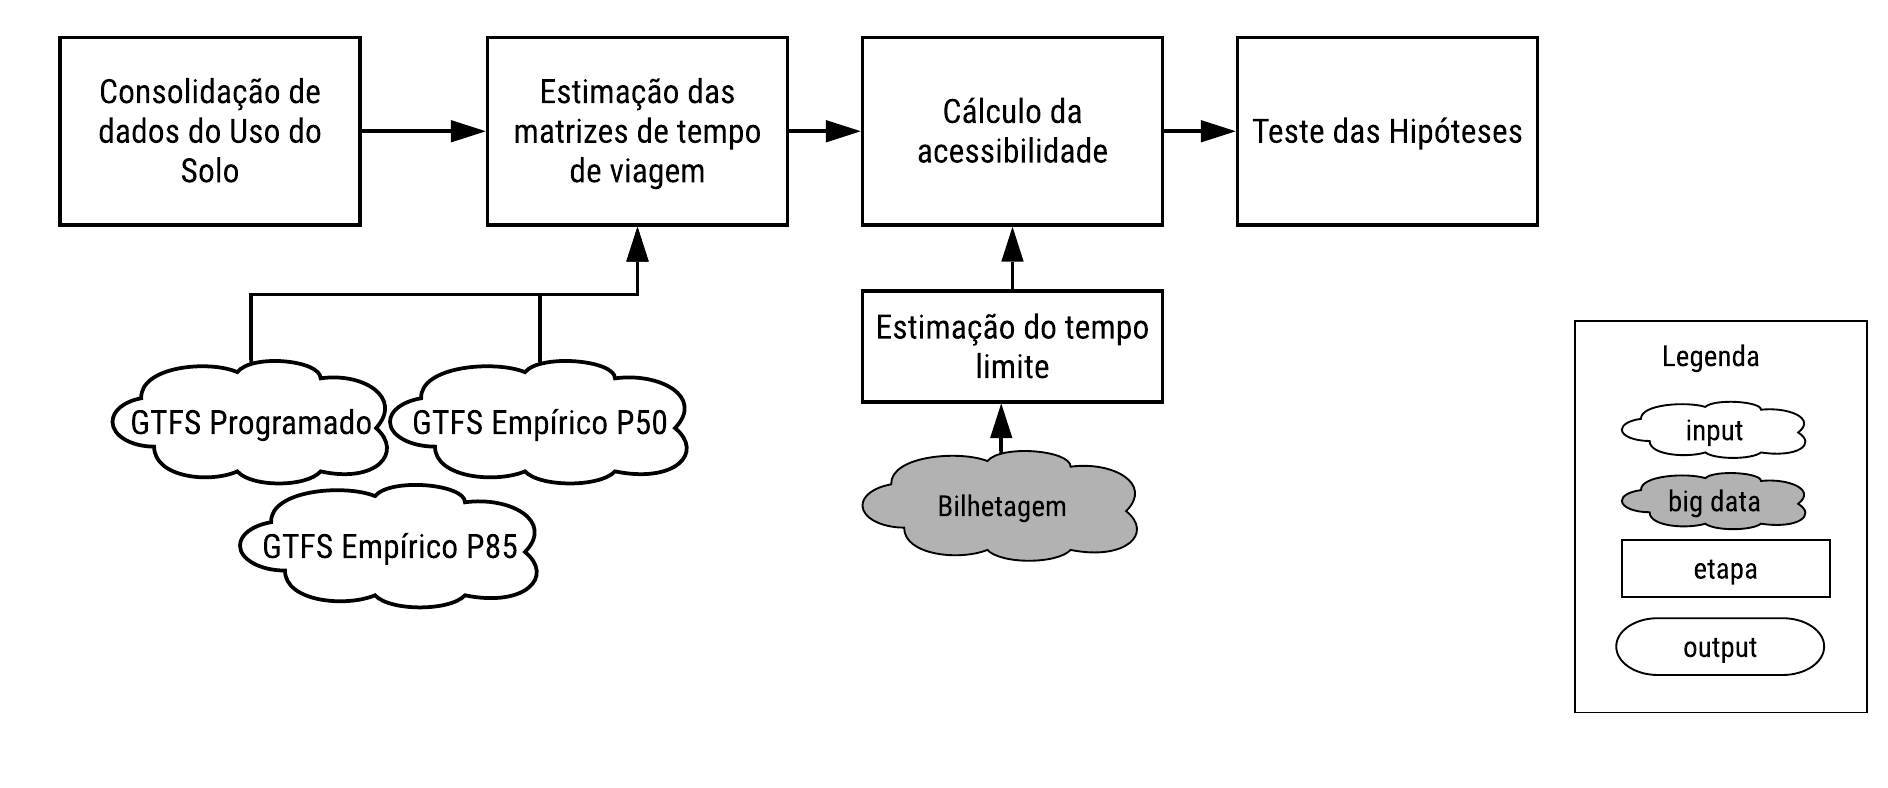
\includegraphics[width=16cm, keepaspectratio]{figure/4-metodologia_parte2.png}}
  }{
  \Fonte{Elaborada pelo autor}
  }
  \end{figure}
  
  \hypertarget{consolidacao-de-dados-do-uso-do-solo-e-agregacao-espacial}{%
  \subsection{Consolidação de dados do uso do solo e agregação espacial}\label{consolidacao-de-dados-do-uso-do-solo-e-agregacao-espacial}}
  
  É necessário consolidar dados de empregos e educação para o cálculo dos indicadores de acessibilidade para essas atividades. Dados de empregos são advindos da Relação Anual de Informações Sociais (RAIS) (Ministério do Trabalho), do ano de 2017, que detém dados de vínculos formais no Brasil.
  
  Os dados da RAIS disponibilizados junto ao IPEA (Instituto de Pesquisa Econômica Aplicada) apresentam um pré-tratamento que busca eliminar outliers que possam indicar uma concentração indevida de empregos em certos locais. É conhecido que, na base da RAIS, a localização da maioria dos serviços públicos é concentradas em endereços que representam a categoria do serviço. Por exemplo, a maioria dos profissionais de educação do estado são concentrados no endereço da secretaria de educação do estado.
  
  Dados de educação são do Censo Escolar de 2015, que apresenta diversas informações sobre cada escola no Brasil, como sua localização, se é público ou privada, e a quantidade de matrículas em cada segmento do ensino (ensino infantil, ensino fundamental e ensino médio). Para esse trabalho, serão consideradas as matrículas para ensino infantil, fundamental e médio de todas as escolas públicas (municipais, estaduais e federais) de Fortaleza.
  
  \hypertarget{estimacao-das-matrizes-de-tempo-de-viagem}{%
  \subsection{Estimação das matrizes de tempo de viagem}\label{estimacao-das-matrizes-de-tempo-de-viagem}}
  
  A estimação das matrizes busca subsidiar o cálculo de indicadores de acessibilidade que serão utilizados para avaliar três hipóteses levantadas como integrantes das questões de pesquisas nesse trabalho: 1) há um diferença entre a acessibilidade estimada pelas tabela de horários programados e a estimada pela tabela de horários empíricos, e 2) há uma diferença entre a acessibilidade estimada para tempos de viagem entre paradas medianos (GTFS Empírico P50) e a estimada para tempos de viagem entre paradas extremos (GTFS Empírico P85) e 3) há uma diferença de acessibilidade entre os horários de partida. Essa última hipótese já foi bastante discutida na literatura, \citep{Stepniak2019, Owen2015}. Isso acontece porque, para viagens de transporte público, até pequenas diferenças no horário do começo da viagem (domicílio) podem implicar em grande diferenças no tempo total de viagem, principalmente através da perda de integrações e elevados tempos de espera \citep{Stepniak2019}
  
  Para mostrar a importância da utilização dos tempos de viagens empíricos para análises de acessibilidade, é feita a estimação do tempo de viagem entre pares origem-destino. Para esse fim, são utilizadas as agregações espaciais H3 desenvolvidas pelo Uber (Figura \ref{fig:uber_h3}). A agregação escolhida é um hexágono que tem tamanho de diagonal menor igual a 357 metros, o que possibilita analisar de forma desagregada a variação da acessibilidade. Já foi mostrado que esse tipo de agregação é capaz de mostrar algumas tendências de acessibilidade (como acessibilidade maior perto de corredores de média/alta capacidade) que outras agregações maiores não conseguem \citep{Pereira2019}.
  
  \begin{figure}[!h]
  \captionsetup{width=16cm}
  \Caption{\label{fig:uber_h3}Agregações hexagonais H3}
  \centering
  \UFCfig{}{
  {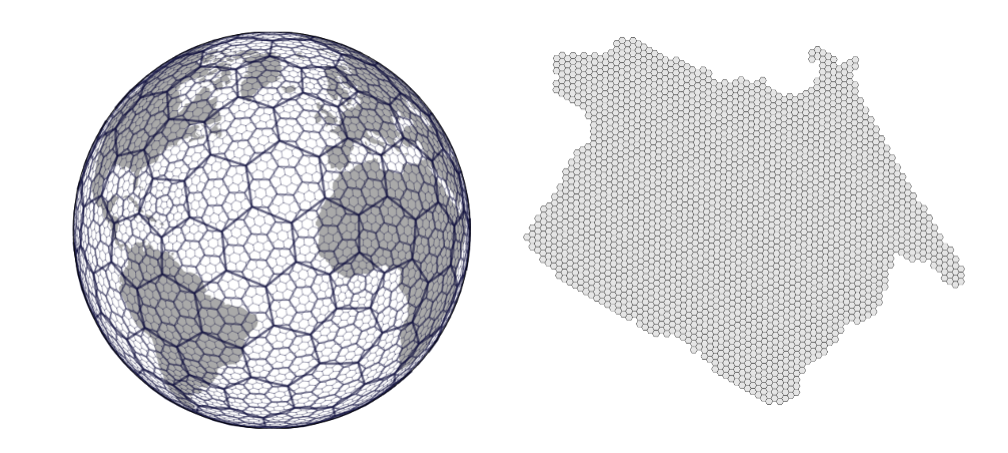
\includegraphics[width=16cm, keepaspectratio]{figure/4-uber_h3_for_h3.png}}
  }{
  \Fonte{Elaborada pelo autor}
  }
  \end{figure}
  
  Portanto, para a avaliação da hipótese 1, serão estimadas 5 matrizes de tempo de viagem entre cada um dos pares origem destino de Fortaleza entre 6h45 e 7h45 da manhã, uma cada 15 minutos, para o GTFS Programado e para o GTFS Empírico P50. Para a hipótese 2, serão estimadas mais 5 matrizes de tempo de viagem a cada 15 minutos entre entre 6h45 e 7h45 da manhã para o GTFS Empírico P85. No total, serão estimada 8 matrizes para a hipótese 1 e mais 4 para a hipótese 2.
  
  Para a estimação do tempo de viagem, foi escolhido o \emph{OpenTripPlanner}. A sua escolha foi feita por algumas razões: 1) é um aplicativo completamente gratuito, open source e sem limitação de uso; 2) integra facilmente com as demais ferramentas utilizadas nesse trabalho (principalmente o R); 3) é de uso constante do autor há alguns meses. A ferramenta considera todas as etapas do deslocamento no seu roteamento: o tempo de caminhada até a parada, o tempo de espera, o tempo no veículo e o tempo de espera em possíveis integrações.
  
  Atualmente, a utilização do OTP em massa pode ser feita de duas formas (principais): 1) através de consultas feitas a um servidor local e 2) através de um API que liga o Java diretamente ao Python. A primeira forma é capaz de retornar como resultado um passo a passo completo do itinerário para o par origem-destino escolhido, com os tempos de espera, caminhada, dentro do veículo, e a linha de cada etapa por transporte público. A segunda forma retorna informações somente de tempo total de viagem e distância de caminhada, porém apresenta uma velocidade de processamento que pode chegar até 20x mais rápida que a primeira alternativa.
  
  A utilização dos hexágonos de diagonal menor de 357 metros resulta em 2760 hexágonos para a cidade de Fortaleza, sendo o roteamento feito a partir do centróide de cada hexágono. Isso implica num total de 7,7 milhões de pares origem-destino, e para 12 consultas em hora pico isso resulta em mais de 92 milhões de consultas de tempo de viagem. Tendo em vista esse volume, a segunda opção foi selecionada como sendo a mais viável.
  
  O OTP permite que sejam determinados alguns parâmetros para o seu roteamento. Dentre eles, o principal é o da distância máxima de caminhada, que para esse trabalho foi estabelecida como 800 metros. Essa distância, entretanto, não é respeitada caso a única alternativa para o usuário seja uma caminhada maior que o limite.
  
  Para tornar o roteamento mais eficiente, hexágonos que não tiveram nenhuma população ou atividade serão excluídas da análise, sendo entendido que estas não serão origem ou destino para nenhuma atividade.
  
  Com as matrizes de tempo de viagem estimadas, é passado para etapa que vai calcular os indicadores de acessibilidade.
  
  \hypertarget{calculo-da-acessibilidade}{%
  \subsection{Cálculo da acessibilidade}\label{calculo-da-acessibilidade}}
  
  O indicador escolhido para testar as hipóteses do trabalho é o indicador de acessibilidade cumulativa. Esse indicador, de fácil compreensão, estima a quantidade de oportunidades que podem ser alcançadas dado um certo tempo de viagem limite. Esse indicador foi utilizado em vários dos trabalhos citados neste texto \citep{Wessel2017, Owen2015, Pereira2019}.
  
  De acordo com a classificação estabelecida por \citet{Geurs2004}, essa medida consegue incorporar os componentes de transporte e uso do solo, e o seu cálculo para diferentes horários de partida na hora pico também incorpora o componente temporal.
  
  Como limitação, o indicador aqui utilizado assume que todas as oportunidades são igualmente desejáveis pelos viajantes. É assumido que uma escola a 1km da sua casa tem o mesmo peso que uma escola a 5km, por exemplo. Além disso, não incorpora a competição que há por essas atividades.
  
  Portanto, são calculados indicadores de acessibilidade cumulativa para duas atividades: trabalho e educação. As atividades de trabalho são representadas pela quantidade de vínculos empregatícios ativos coletados da RAIS, enquanto que as atividades de educação são representadas pela quantidade de matrículas de ensino infantil, médio e fundamental somados.
  
  Como dito, é necessário o estabelecimento de um tempo limite de viagem para o cálculo desse indicador. A abordagem tradicional estipula esse tempo muitas vezes baseado no que ele deveria ser, e não no que realmente acontece no sistema. É proposto então o uso dos dados de bilhetagem para esse fim.
  
  \hypertarget{estimacao-do-tempo-limite}{%
  \subsection{Estimação do tempo limite}\label{estimacao-do-tempo-limite}}
  
  Indicadores cumulativos precisam de uma informação de tempo limite para sua estimação. A abordagem predominante na literatura assume tempos limites que variam entre 30 e 90 minutos. A metodologia escolhida aqui parte para a estimação de um indicador positivo, onde serão utilizadas as informações de viagens realizadas pelos usuários advindas dos dados de bilhetagem.
  
  Será, então, calculado o tempo de viagem para cada viagem que foi realizada em hora pico para os motivos de trabalho (viagens realizadas com vale transporte) e para motivo de educação (viagens realizadas por carteira de estudante). Foi escolhido o dia 12 de setembro de 2019 como um dia típico, que está dentro do intervalo de dados que já foi consolidado.
  
  Os dados consolidados de bilhetagem apresentaram uma falha da localização de parte das suas validações. Por isso, a primeira etapa do método consiste em deletar os usuários que tiveram pelo menos uma validação não localizada em seu diário. Em seguida, são filtradas somente as validações por vale transporte e por carteira de estudante.
  
  Como determinado na metodologia, os dados utilizados de educação serão do censo escolar, que só englobam escolas de ensino infantil, fundamental ou médio. Os dados de bilhetagem para carteira de estudante, entretanto, apresentam informações de viagens de todos os usuários, incluindo usuários que acessam oportunidades de educação do ensino superior. Para corrigir isso, foi feita uma consulta à base de registros dos usuários do bilhete único, filtrando somente os usuários de carteira de estudante que nasceram após o ano 2000, que aproximadamente representaria estudantes até o fim do ensino médio. Esses usuários então foram filtrados na base da bilhetagem. Como foi visto na parte da consolidação, há uma falta de correspondência entre as bases da bilhetagem e do cadastro único, então esse tipo de integração acabará diminuindo o tamanho da amostra disponível.
  
  Para a estimação dos tempos de viagem, então, são filtrados aqueles usuários que realizaram a primeira viagem no período do pico da manhã (antes das 8h), que viajaram pelo menos duas vezes e que tiveram um tempo mínimo de 3h entre validações. Esse último critério busca estabelecer um tempo mínimo para cada atividade e excluir validações de integração.
  
  Garantidas essas condições, é então estabelecido que a localização da primeira viagem é a \textbf{origem} e que a localização da viagem seguinte é o \textbf{destino} do usuário. Isso representa uma aproximação que traz consigo a premissa de que o usuário não realizou nenhum trecho que não fosse por transporte público e a pé entre essas duas viagens. Essa é uma limitação que já foi abordada e contornada bastante na literatura \citep{Trepanier2007, Munizaga2012} com a consolidação do Trip Chaining Method. Para este trabalho, entretanto, é mantida.
  
  Com as origem e destinos determinadas e localizadas, é feita uma associação espacial com os hexágonos escolhidos nas etapas anterior. Com as matrizes de tempo de viagem já estimadas, é então sabido o tempo de viagem entre cada uma das origens e destinos obtidos. Para isso, é utilizada a matriz de tempo de viagem a partir do GTFS Corrigido.
  
  Isso então oferece o tempo de viagem do pico manhã para cada um dos usuários que se encaixou nos critérios estabelecidos. Determina-se então que o tempo limite é o \textbf{percentil 75} do tempo de viagem para cada um dos motivos de viagem (trabalho e educação). Isso é feito entendendo que esse tempo tende a ser diferente para as atividades.
  
  \hypertarget{teste-das-hipoteses}{%
  \subsection{Teste das hipóteses}\label{teste-das-hipoteses}}
  
  Por fim, é feita uma análise comparativa para avaliar as três hipóteses definidas neste trabalho. O teste das hipóteses é feito de forma descritiva, analisando valores absolutos e relativos de variação. A Figura \ref{fig:metologia_teste_hip} ilustra as hipóteses e qual indicador vai ser avaliado. É importante ressaltar que o GTFS Empírico P50 é aqui considerado como o que representa o estado mediano do sistema. Ele é o que representa o valor ``corrigido'' do GTFS Programado. Também é utilizado o termo ``cenário'' para identificar cada lado de uma hipótese.
  
  \begin{figure}[!h]
  \captionsetup{width=16cm}
  \Caption{\label{fig:metologia_teste_hip}Hipóteses a serem testadas}
  \centering
  \UFCfig{}{
  {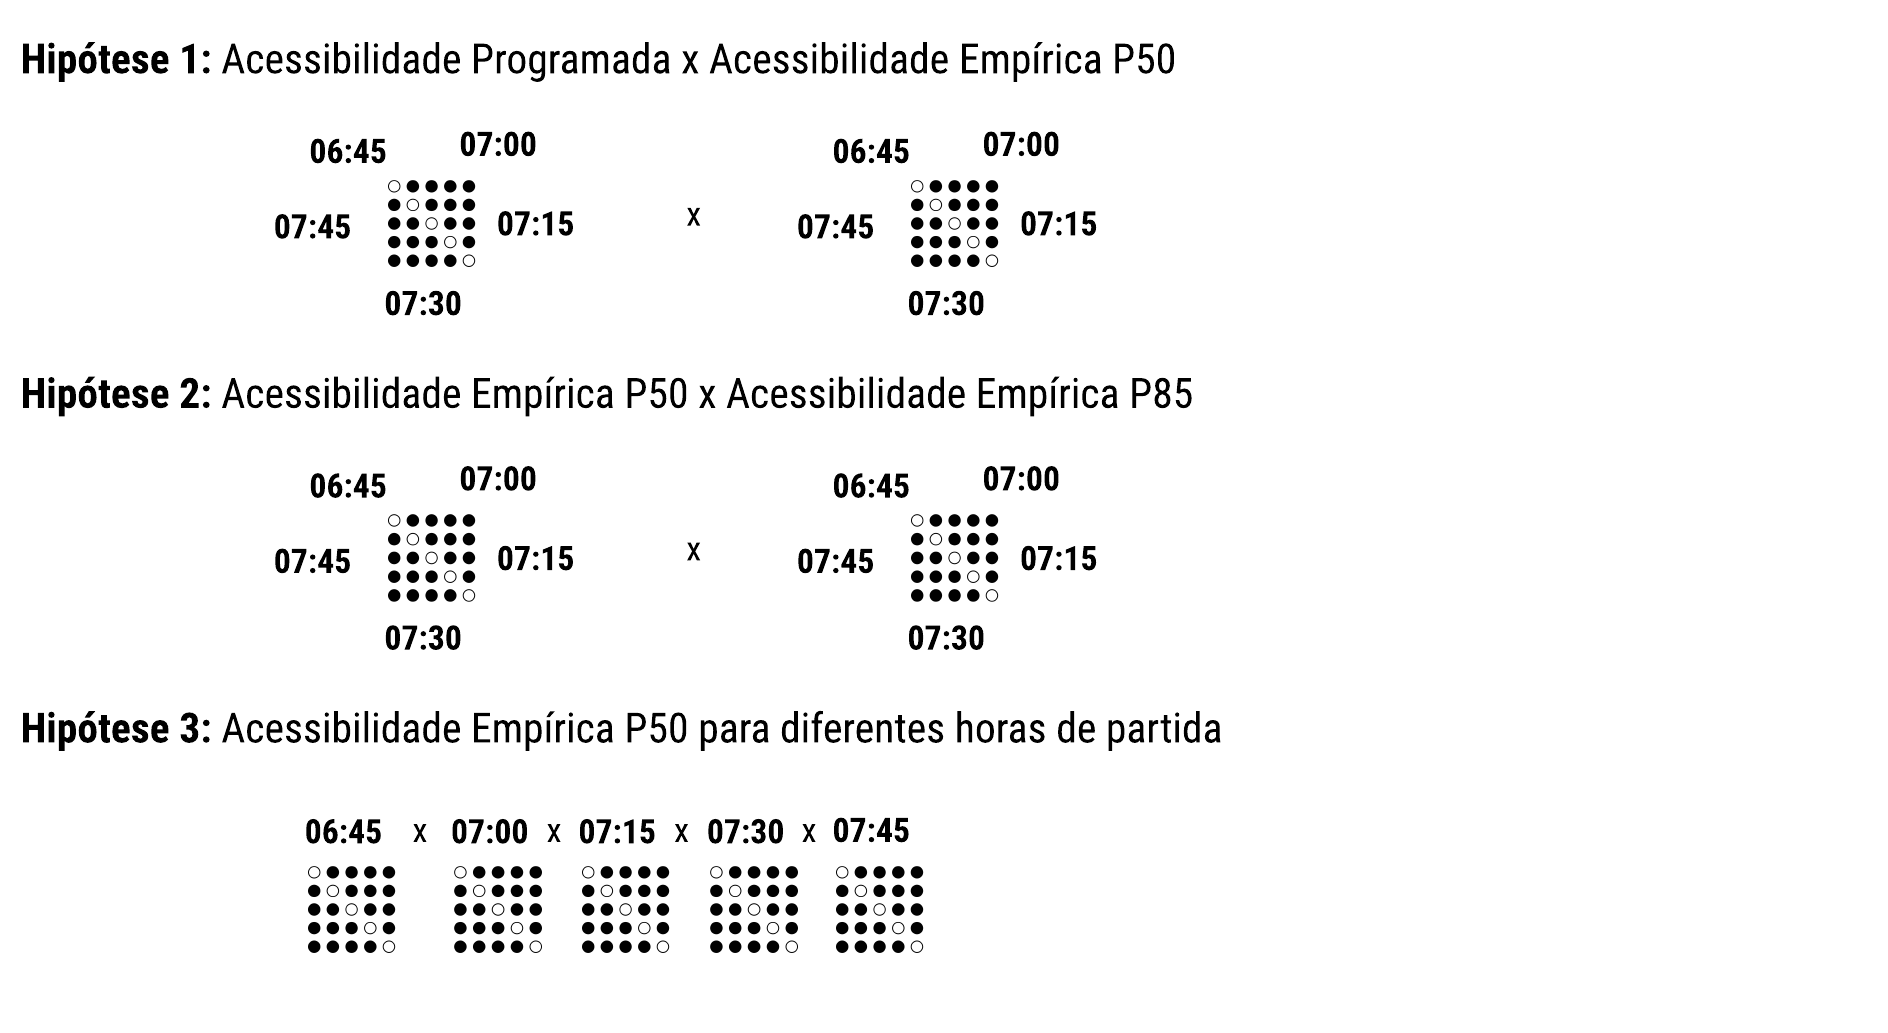
\includegraphics[width=16cm, keepaspectratio]{figure/4-metodologia_teste_hipoteses.png}}
  }{
  \Fonte{Elaborada pelo autor}
  }
  \end{figure}
  
  Primeiramente, para avaliar a diferença entre a acessibilidade pelo GTFS Programado e o GTFS Corrigido, é feita uma comparação não-espacial dos valores de acessibilidade estimados para todos os hexágonos para o caso do GTFS Programado e do GTFS Corrigido, para as atividades de trabalho e educação. Como para ambos os GTFS foram calculadas matrizes para 5 tempos de partida, os indicadores são calculados em torno de uma matriz da mediana do tempo de viagem (n = 5).
  
  Em seguida, a diferença relativa entre os dois indicadores é mostrada no mapa. Como a variação da acessibilidade pode ser negativa ou positiva, o indicador escolhido será a divisão do logaritmo da acessibilidade corrigida pelo logaritmo da acessibilidade programada.
  
  Para a diferença absoluta, é também analisada a distribuição espacial e não-espacial do indicador. Para fazer uma comparação entre as atividades, a distribuição não-espacial é analisada através da porcentagem da diferença absoluta em relação ao total de atividades na cidade. Por exemplo, hipoteticamente falando, será mostrado que certo hexágono perde 10\% do total de empregos da cidade ou 5\% do total de matrículas quando é utilizado o GTFS Programado em vez do GTFS Corrigido. Esse indicador resumidamente responde à pergunta ``qual a proporção de empregos/matrículos da cidade que não são mais acessíveis?''
  
  Para a hipótese 2, é feita uma comparação de como a acessibilidade varia levando em conta os diferentes cenários de variabilidade de tempo de viagem. Primeiramente, é feita uma comparação visual dos mapas da acessibilidade para tempos medianos (GTFS Empírico P50) e para tempos de dispersão (GTFS Empírico P85). Em seguida, é analisada a variação absoluta da acessibilidade. Mais uma vez, os indicadores são calculados em torno de uma matriz da mediana dos tempos de viagem (n = 5) para as atividades de emprego e educação. Similar à análise feita na hipótese 1, a diferença absoluta também será analisada como o percentual em relação ao total de atividades na cidade.
  
  Para essas duas hipótese também é feita uma análise da área de influência de algumas agregações críticas de acessibilidade. São selecionados hexágonos que estejam em áreas de média/alta densidade e que tenha uma grande variabilidade de acessibilidade entre os cenários. A área de influência é representada pelos hexágonos que cada um dos hexágonos críticos conseguem alcançar.
  
  Por fim, é feita uma análise de como a acessibilidade pode variar para diferentes horários de partida, dentro da hora pico. Para isso, será utilizado o coeficiente de variação da acessibilidade (P50) da amostra coletada de tempo de saída (06:45 à 07:45, cada 15 minutos). O indicador no mapa permite ver onde o impacto do tempo de partida é maior, com a limitação principal sendo do tamanho pequeno da amostra (n = 5 horários de partidas).
  
  O tamanho da amostra de coleta dos tempos de viagem pode ser considerada a principal limitação dessa metodologia de avaliação das hipóteses. Em virtude do alto tempo de processamento na produção das matrizes, foi identificado um \emph{tradeoff} entre a resolução espacial e temporal. Neste trabalho, foi escolhida a resolução espacial como prioridade, principalmente em virtude do que é feito na literatura: enquanto resoluções temporais maiores já foram exploradas, pouco foi feito utilizando uma resolução espacial maior. A resolução espacial maior permite, por exemplo, identificar como a acessibilidade é maior perto de corredores de transporte público, e como a variação dela também é menor nessas áreas.
  
  O método para testar as hipóteses baseia-se na comparação visual e de medidas descritivas como mediana, percentis e coeficiente de variação. Entende-se, entretanto, que essa análise apresenta limitações, visto principalmente que estamos tratando de um fenômeno que tem conhecido caráter de dependência espacial.
  
  \hypertarget{consideracoes-finais-2}{%
  \section{Considerações finais}\label{consideracoes-finais-2}}
  
  É importante ressaltar que a estimação dos tempos de viagem entre pares origem destino pode falhar na captação de algumas peculiaridades culturais e sistemáticas de um sistema de transporte público. Em Fortaleza, por exemplo, a consolidação de 7 grandes terminais de integração tornaram esses pontos quase como paradas obrigatórias na integração das viagens dos usuários. A oferta do sistema em si, construído numa configuração tronco-alimentadora, já leva os usuários a fazerem a integração no terminal. Soma-se isso à sensação de segurança e conforto proporcionada pelos terminais, levando à uma grande utilização dos mesmos, mesmo que isso represente um acréscimo no tempo de viagem do usuário. No roteamento do OTP, entretanto, os terminais são considerados pontos de parada como todos os outros, e a rota retornada sempre será aquele de menor desutilidade, que, no caso, é a de menor tempo.
  
  Outra limitação importante é a não incorporação das linhas de média/alta capacidade. Isso deu ao fato dessas linhas ainda não serem integradas ao sistema, nem tarifariamente e nem operacionalmente. Além disso, a frequência dessas linhas é bem baixa, o que pode comprometer a sua qualificação como ``alta capacidade''. A Linha Sul, que vai da região metropolitana ao centro da cidade, tem intervalo maiores que 15 minutos. A Linha Oeste, que tem características parecidas, tem intervalo maior que 30 minutos. O novo VLT ainda está em processo de implementação, funcionando em operação assistida só em hora pico.
  
  A implementação da metodologia proposta traz alguns desafios, sendo o principal de ordem computacional. O processamento dos dados de GPS (já separados por dia) pode ser feito em um computador pessoal, mas etapas como a agregação dos tempos de viagens de todos os dias e a estimação das matrizes de tempo de viagem entre pares origem-destino requer máquinas de médio/alto poder de processamento para uma geração de resultados em um tempo razoável. Esse alto tempo de processamento somado ao cronograma limitado de uma pesquisa de mestrado levou à tomada de decisões que impuseram limites à metodologia do trabalho, como destacado acima no \emph{tradeoff} entre a resolução espacial e a resolução temporal da análise. A implementação da metodologia acontece no próximo capítulo.
  
  \hypertarget{discussao-dos-resultados}{%
  \chapter{Discussão dos resultados}\label{discussao-dos-resultados}}
  
  Este capítulo busca alcançar os três últimos objetivos do trabalho, mostrando os principais resultados advindos da aplicação do método do capítulo anterior e a importância do mesmo. Os resultados são apresentados e as hipóteses são discutidas individualmente, analisando o impacto da variabilidade da acessibilidade na avaliação de políticas públicas. Por fim, é feita uma discussão geral dos resultados com a análise de como os resultados encontrados nesse capítulo se diferem dos encontrados na literatura.
  
  \hypertarget{reconstrucao-da-tabela-de-horarios-programados-do-gtfs-para-diferentes-cenarios-1}{%
  \section{Reconstrução da tabela de horários programados do GTFS para diferentes cenários}\label{reconstrucao-da-tabela-de-horarios-programados-do-gtfs-para-diferentes-cenarios-1}}
  
  O método do capítulo anterior é então aplicado para 19 dias úteis de setembro/2018 de dados consolidados de GPS, bilhetagem, GTFS e registros dos usuários. Os tópicos abaixo apresentam os principais resultados da aplicação
  
  \hypertarget{definicao-do-momento-de-passagem-em-cada-parada-e-deteccao-de-outliers}{%
  \subsection{Definição do momento de passagem em cada parada e detecção de outliers}\label{definicao-do-momento-de-passagem-em-cada-parada-e-deteccao-de-outliers}}
  
  A Figura \ref{fig:outliers_interp} mostra um caso onde é provada a aplicação do método para excluir outliers. O eixo x mostra a distância acumulada ao longo do trajeto, com o eixo y mostrando ao momento. O exemplo é de um veículo da linha 86, no sentido da ida. Observa-se, no gráfico de cima, alguns pontos de destoam dos demais. Essa linha tem a peculiaridade de passar na mesma via, em sentido oposto, em momentos diferentes. Como os pontos de GPS podem ser imprecisos no seu registro, alguns tempos que deveriam ter sido alocados a um sentido da via foram a alocados ao sentido oposto, causando os outliers mostrados na figura. O gráfico de baixo mostra a viagem sem os outliers, já com as paradas da linha que foram interpoladas linearmente.
  
  \begin{figure}[!h]
  \captionsetup{width=16cm}
  \Caption{\label{fig:outliers_interp}Exemplo de interpolação das paradas e remoção dos outliers}
  \centering
  \UFCfig{}{
  {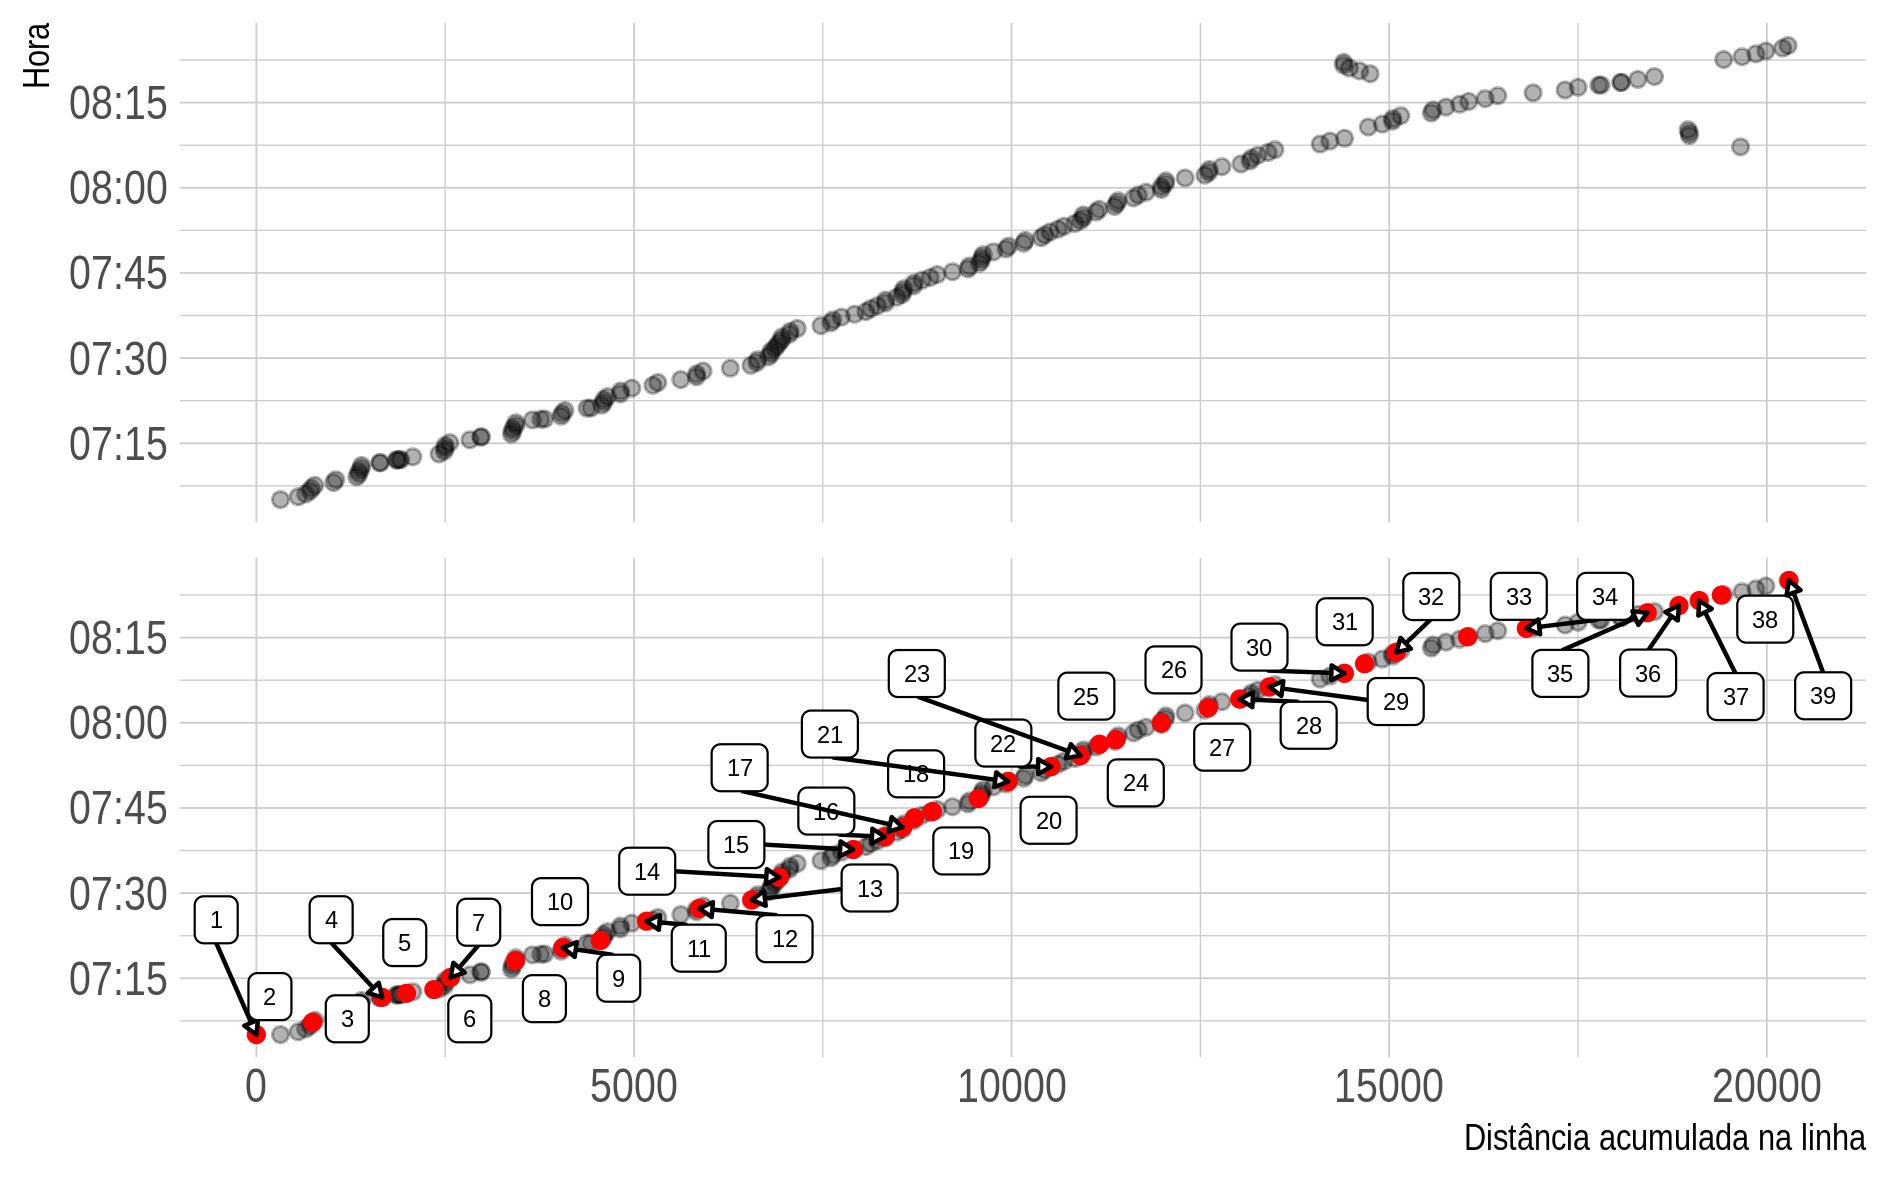
\includegraphics[width=16cm, keepaspectratio]{figure/5-outliers_interpolacao.png}}
  }{
  \Fonte{Elaborada pelo autor}
  }
  \end{figure}
  
  De acordo com os dados de GTFS, o SIT-FOR apresenta 5713 trechos percorridos por veículos (sem contar com trechos percorridos por linhas corujões e expressos). Desse total, cerca de 330 trechos não tiveram tempo de viagem estimado. A principal razão para esse número é a falta de dados de tempo de viagem para linhas complementares, que funcionam principalmente no sistema alimentador onde são as únicas linhas trafegando por certos trechos. Segundo, algumas linhas comuns (não-expressas) rodam veículos em caráter expresso, especialmente em hora de pico. Esse tipo de trecho (um trecho só que corresponde a toda a viagem) não foi incorporado no método para calcular o tempo de viagem.
  
  Foi estabelecido que a velocidade máxima aceitável em um trecho entre paradas é de 60 km/h, sendo descartado tudo que está acima desse valor. Aplicado esse critério, 0,8\% da base foi descartada, porque:
  
  \begin{itemize}
  \tightlist
  \item
    Havia alguns trechos com deserto de registro de localização do veículo. Isso pode acontecer por dois motivos: devido a um erro do aparelho de GPS ou devido à algum momento em que o veículo tenha saído da sua rota original. Foi então interpolado linearmente nas paradas, o que pode acabar penalizando trechos que tem mais baixa velocidade que outros, ocasionando altas velocidades em alguns deles;
  \item
    Algumas linhas (no mesmo sentido) apresentam trechos que correm muito próximos um dos outros, principalmente em situações em que a linha faz um retorno, voltando para a mesma via, só que em sentido contrário. Juntando isso à imprecisão nos registros de GPS, aconteceram casos em que o registro de localização foi alocado para o lado errado da via, causando uma imprecisão na estimação do tempo de passagem nas paradas;
  \item
    Algumas linhas podem operar em um itinerário diferente do previsto. Quando isso acontece, pode acontecer dela percorrer uma distância menor do que está previsto no seu itinerário, gerando altas velocidades.
  \end{itemize}
  
  No total, foram estimadas cerca de 120000 observações agregadas de combinações de trechos e intervalos. Dessas valor, cerca de 17\% tiveram uma amostra menor que 10 observações, e foram descartadas. Grande parte desses trechos aconteciam nas primeiras viagens, onde a frequência do serviço é menor, gerando uma menor amostra. Da amostra de 85000 da combinação de trechos e intervalos, cerca de 1\% apresentou um coeficiente de variação acima de 100\%, e foram excluídas da análise.
  
  Por fim, a Figura \ref{fig:resultado_trechos} mostra a espacialização da amostra de tempos de viagens nos trechos, para diferentes intervalos de 15 minutos na hora pico. É observado que a amostra cobre bem o sistema, com uma concentração clara em trechos nas regiões centrais. A principal diferença de trechos encontrada entre os intervalos acontece mais em zonas extremas, onde o serviço tem uma frequência baixa, como no sudoeste e no extremos leste da cidade.
  
  \begin{figure}[!h]
  \captionsetup{width=16cm}
  \Caption{\label{fig:resultado_trechos}Trechos com tempo de viagem agregados para os diferentes intervalos}
  \centering
  \UFCfig{}{
  {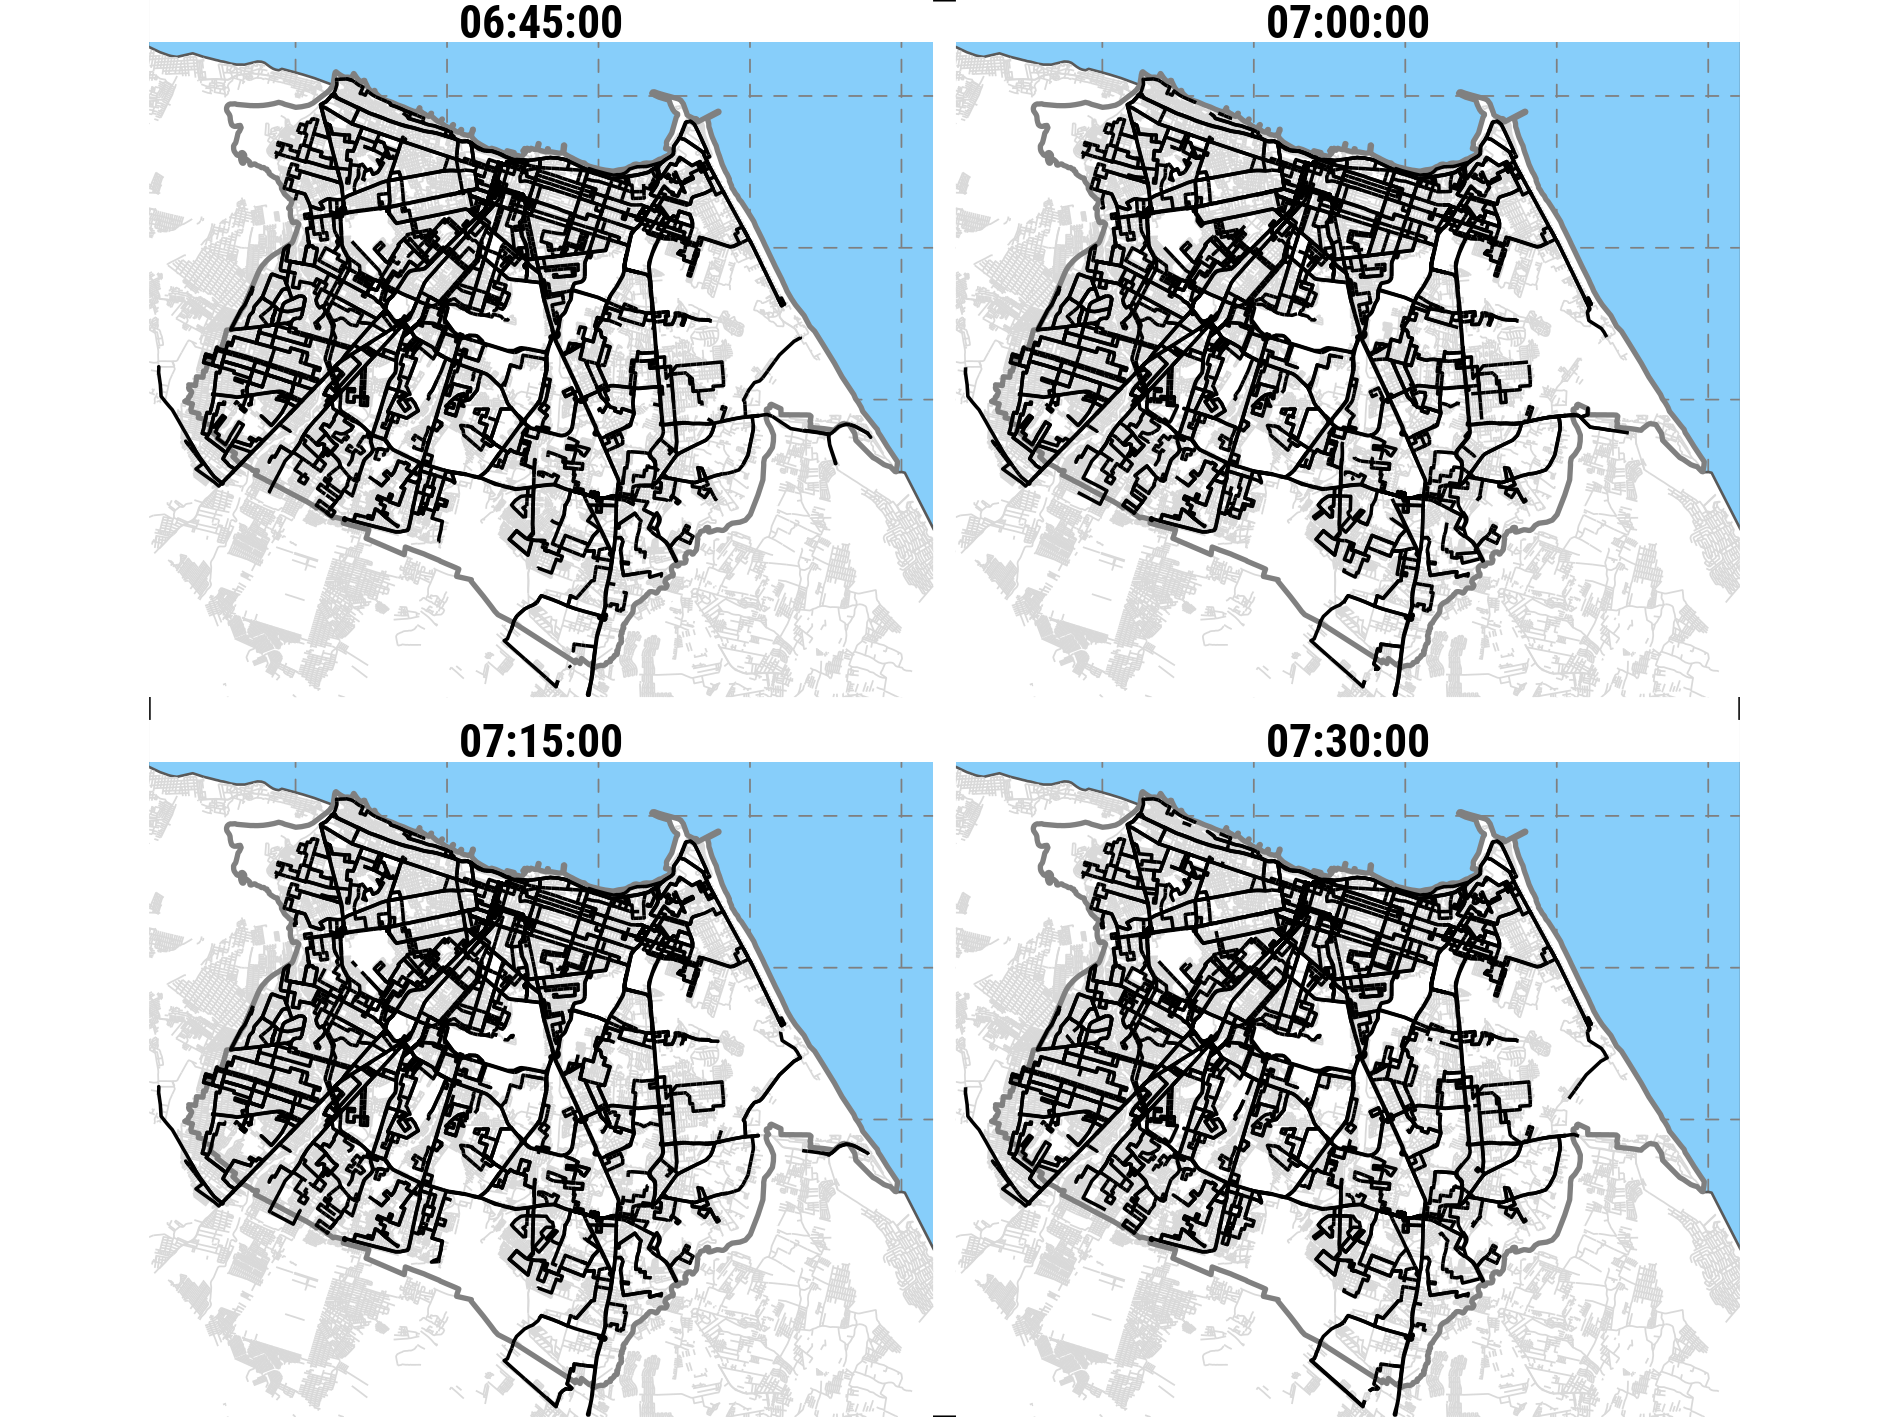
\includegraphics[width=16cm, keepaspectratio]{figure/5-resultado_trechos.png}}
  }{
  \Fonte{Elaborada pelo autor}
  }
  \end{figure}
  
  \hypertarget{reconstrucao-do-arquivo-stop_times-do-gtfs}{%
  \subsection{\texorpdfstring{Reconstrução do arquivo \emph{stop\_times} do GTFS}{Reconstrução do arquivo stop\_times do GTFS}}\label{reconstrucao-do-arquivo-stop_times-do-gtfs}}
  
  Como determinado, foram construídos dois arquivos \emph{stop\_times.txt}: um com a mediana dos tempos de viagem nos trechos (P50) e outro com o percentil 85 (P85). O arquivo \emph{stop\_times.txt} P50 foi considerado como o GTFS Corrigido, que permitia fazer a comparação com o GTFS Programado. A comparação então foi feita analisando o horário programado x horário corrigido de passagem dos veículos por cada parada.
  
  A Figura \ref{fig:resultado_correcao_gtfs} mostra um gráfico de densidade com essa informação. A área na porção inferior no gráfico apresenta horários de passagem em que a hora programada é maior que hora real (o veículo estava adiantado), enquanto que a porção superior apresenta veículos que estão atrasados. A cor mais clara indica que o horário da maior parte dos veículos está próxima do horário programado (próximo das linha vermelha que indica um cenário de perfeita pontualidade).
  
  \begin{figure}[!h]
  \captionsetup{width=16cm}
  \Caption{\label{fig:resultado_correcao_gtfs}Densidade do valor programado x corrigido em cada parada}
  \centering
  \UFCfig{}{
  {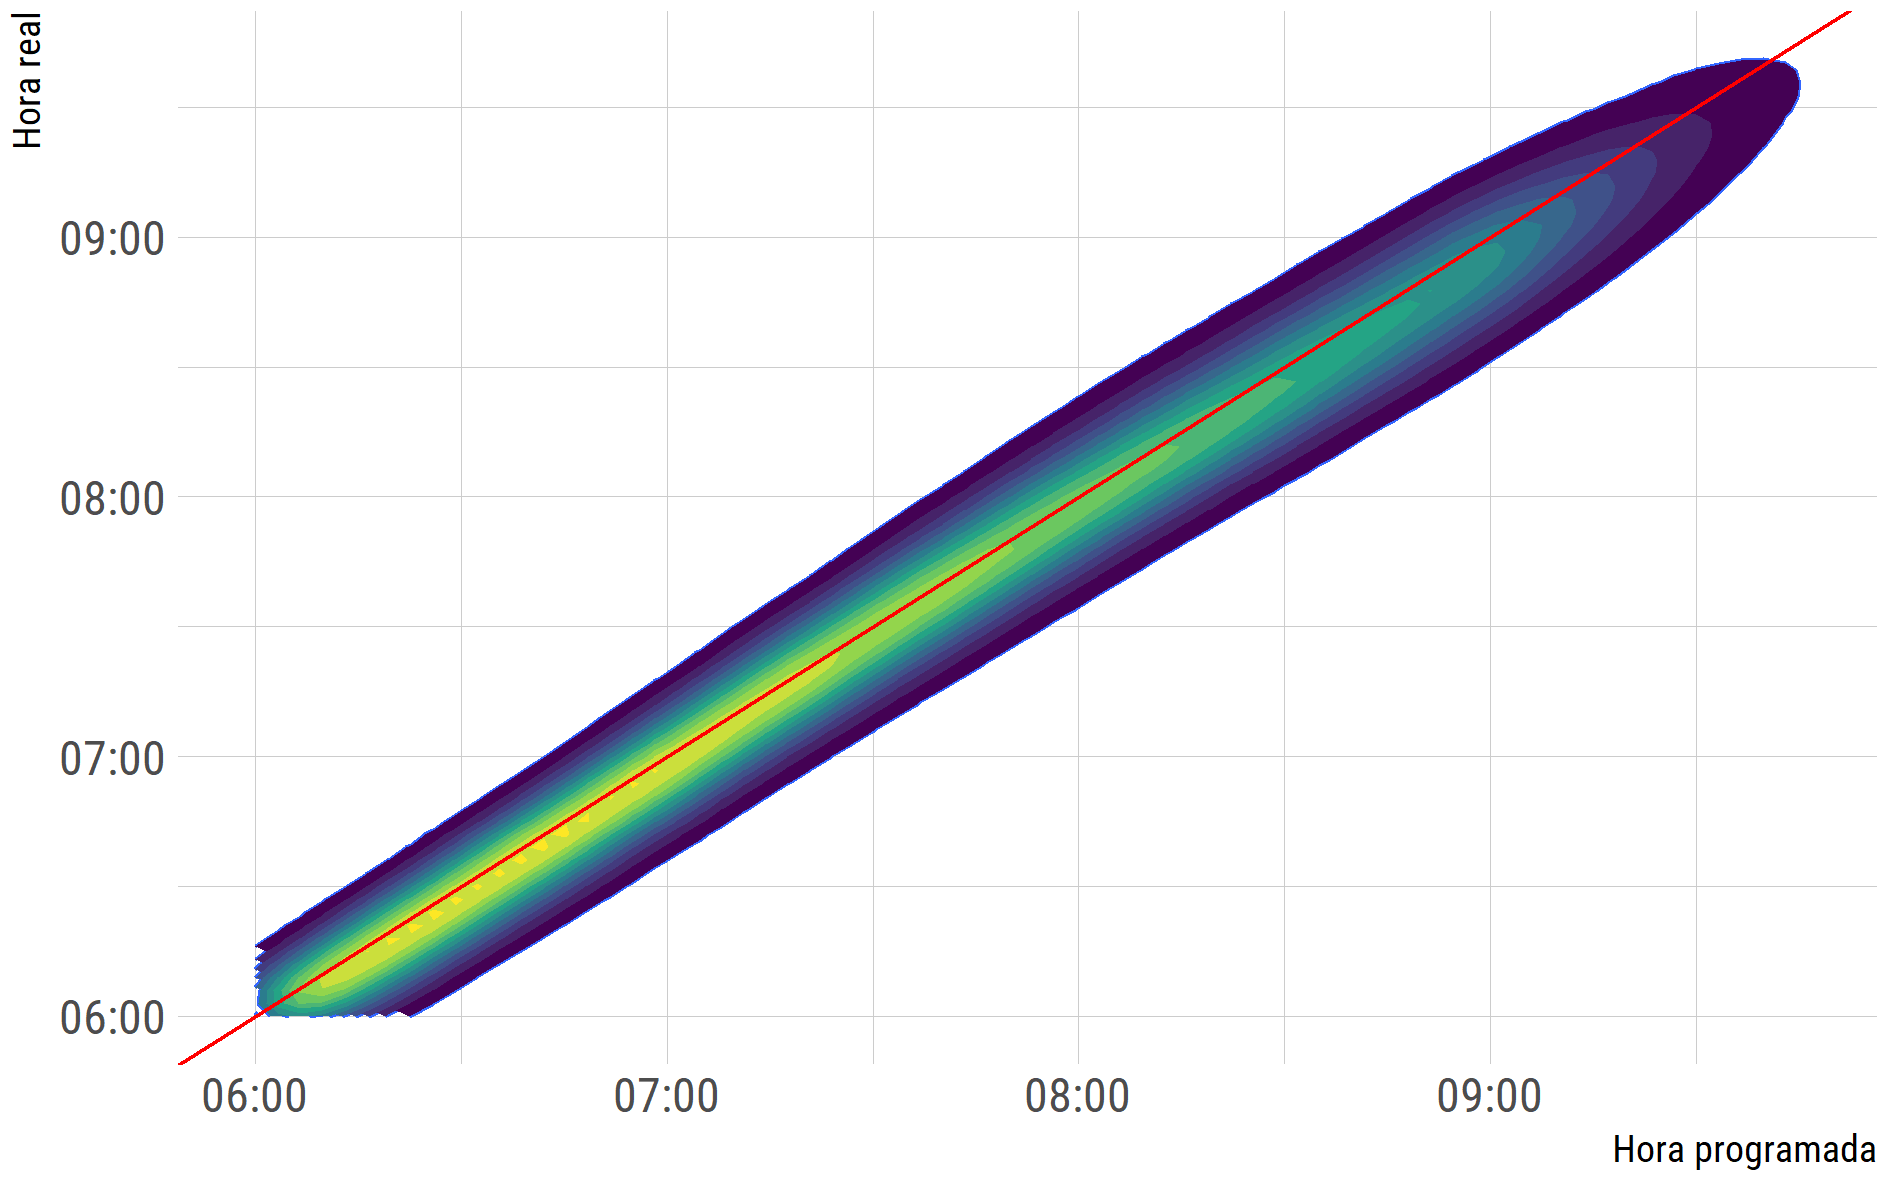
\includegraphics[width=16cm, keepaspectratio]{figure/5-resultado_correcao_gtfs.png}}
  }{
  \Fonte{Elaborada pelo autor}
  }
  \end{figure}
  
  A distribuição da diferença dos horários (real - programado) é mostrada na Figura \ref{fig:resultado_correcao_gtfs_bp}. É mostrado que a variação da diferença é pequena, mas com uma quantidade significativa de \emph{outliers}. Os veículos se adiantam em média 2.7 minutos, com uma mediana de 2 minutos.
  
  \begin{figure}[!h]
  \captionsetup{width=16cm}
  \Caption{\label{fig:resultado_correcao_gtfs_bp}Boxplot da diferença do valor corrigido x programado em cada parada}
  \centering
  \UFCfig{}{
  {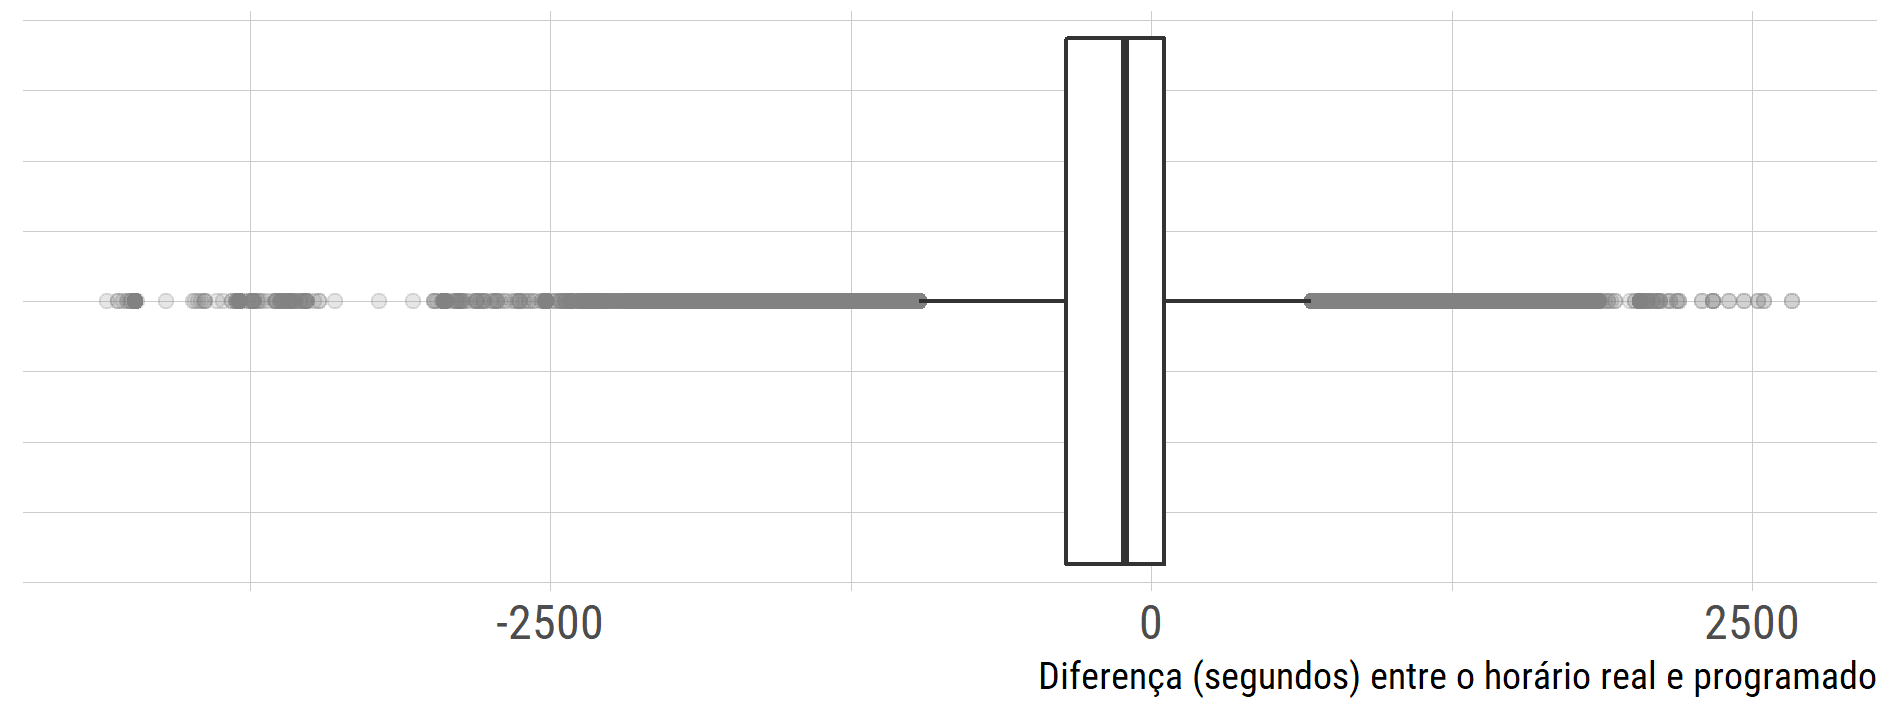
\includegraphics[width=16cm, keepaspectratio]{figure/5-resultado_correcao_gtfs_bp.png}}
  }{
  \Fonte{Elaborada pelo autor}
  }
  \end{figure}
  
  A criação dos GTFS Empíricos P50 e P85 somada ao já existente GTFS Programado permite então avançar no método para a análise comparativa da acessibilidade. A distribuição da pontualidade dos horários apresentou uma pequena variação, mas como a acessibilidade responde a essas variações?
  
  \hypertarget{calculo-da-acessibilidade-1}{%
  \section{Cálculo da acessibilidade}\label{calculo-da-acessibilidade-1}}
  
  Esse tópico mostra os resultados da aplicação do método de cálculo dos indicadores de acessibilidade.
  
  \hypertarget{tratamento-de-dados-do-uso-do-solo}{%
  \subsection{Tratamento de dados do uso do solo}\label{tratamento-de-dados-do-uso-do-solo}}
  
  A Figura \ref{fig:distribuicao_us} mostra a distribuição dos dados de uso do solo consolidados. Os dados de população e renda \emph{per capta} são advindos do Censo 2010 do IBGE, e são apresentados aqui como forma de orientação para possíveis visões da acessibilidade. É importante observar como a concentração de atividades de emprego e de educação se acontece de forma diferente no espaço urbano. Para referência, o total de atividades agregadas para Fortaleza foi de cerca de 550 mil empregos e cerca de 281 mil matrículas.
  
  \begin{figure}[!h]
  \captionsetup{width=16cm}
  \Caption{\label{fig:distribuicao_us}Distribuição espacial das variáveis de uso do solo}
  \centering
  \UFCfig{}{
  {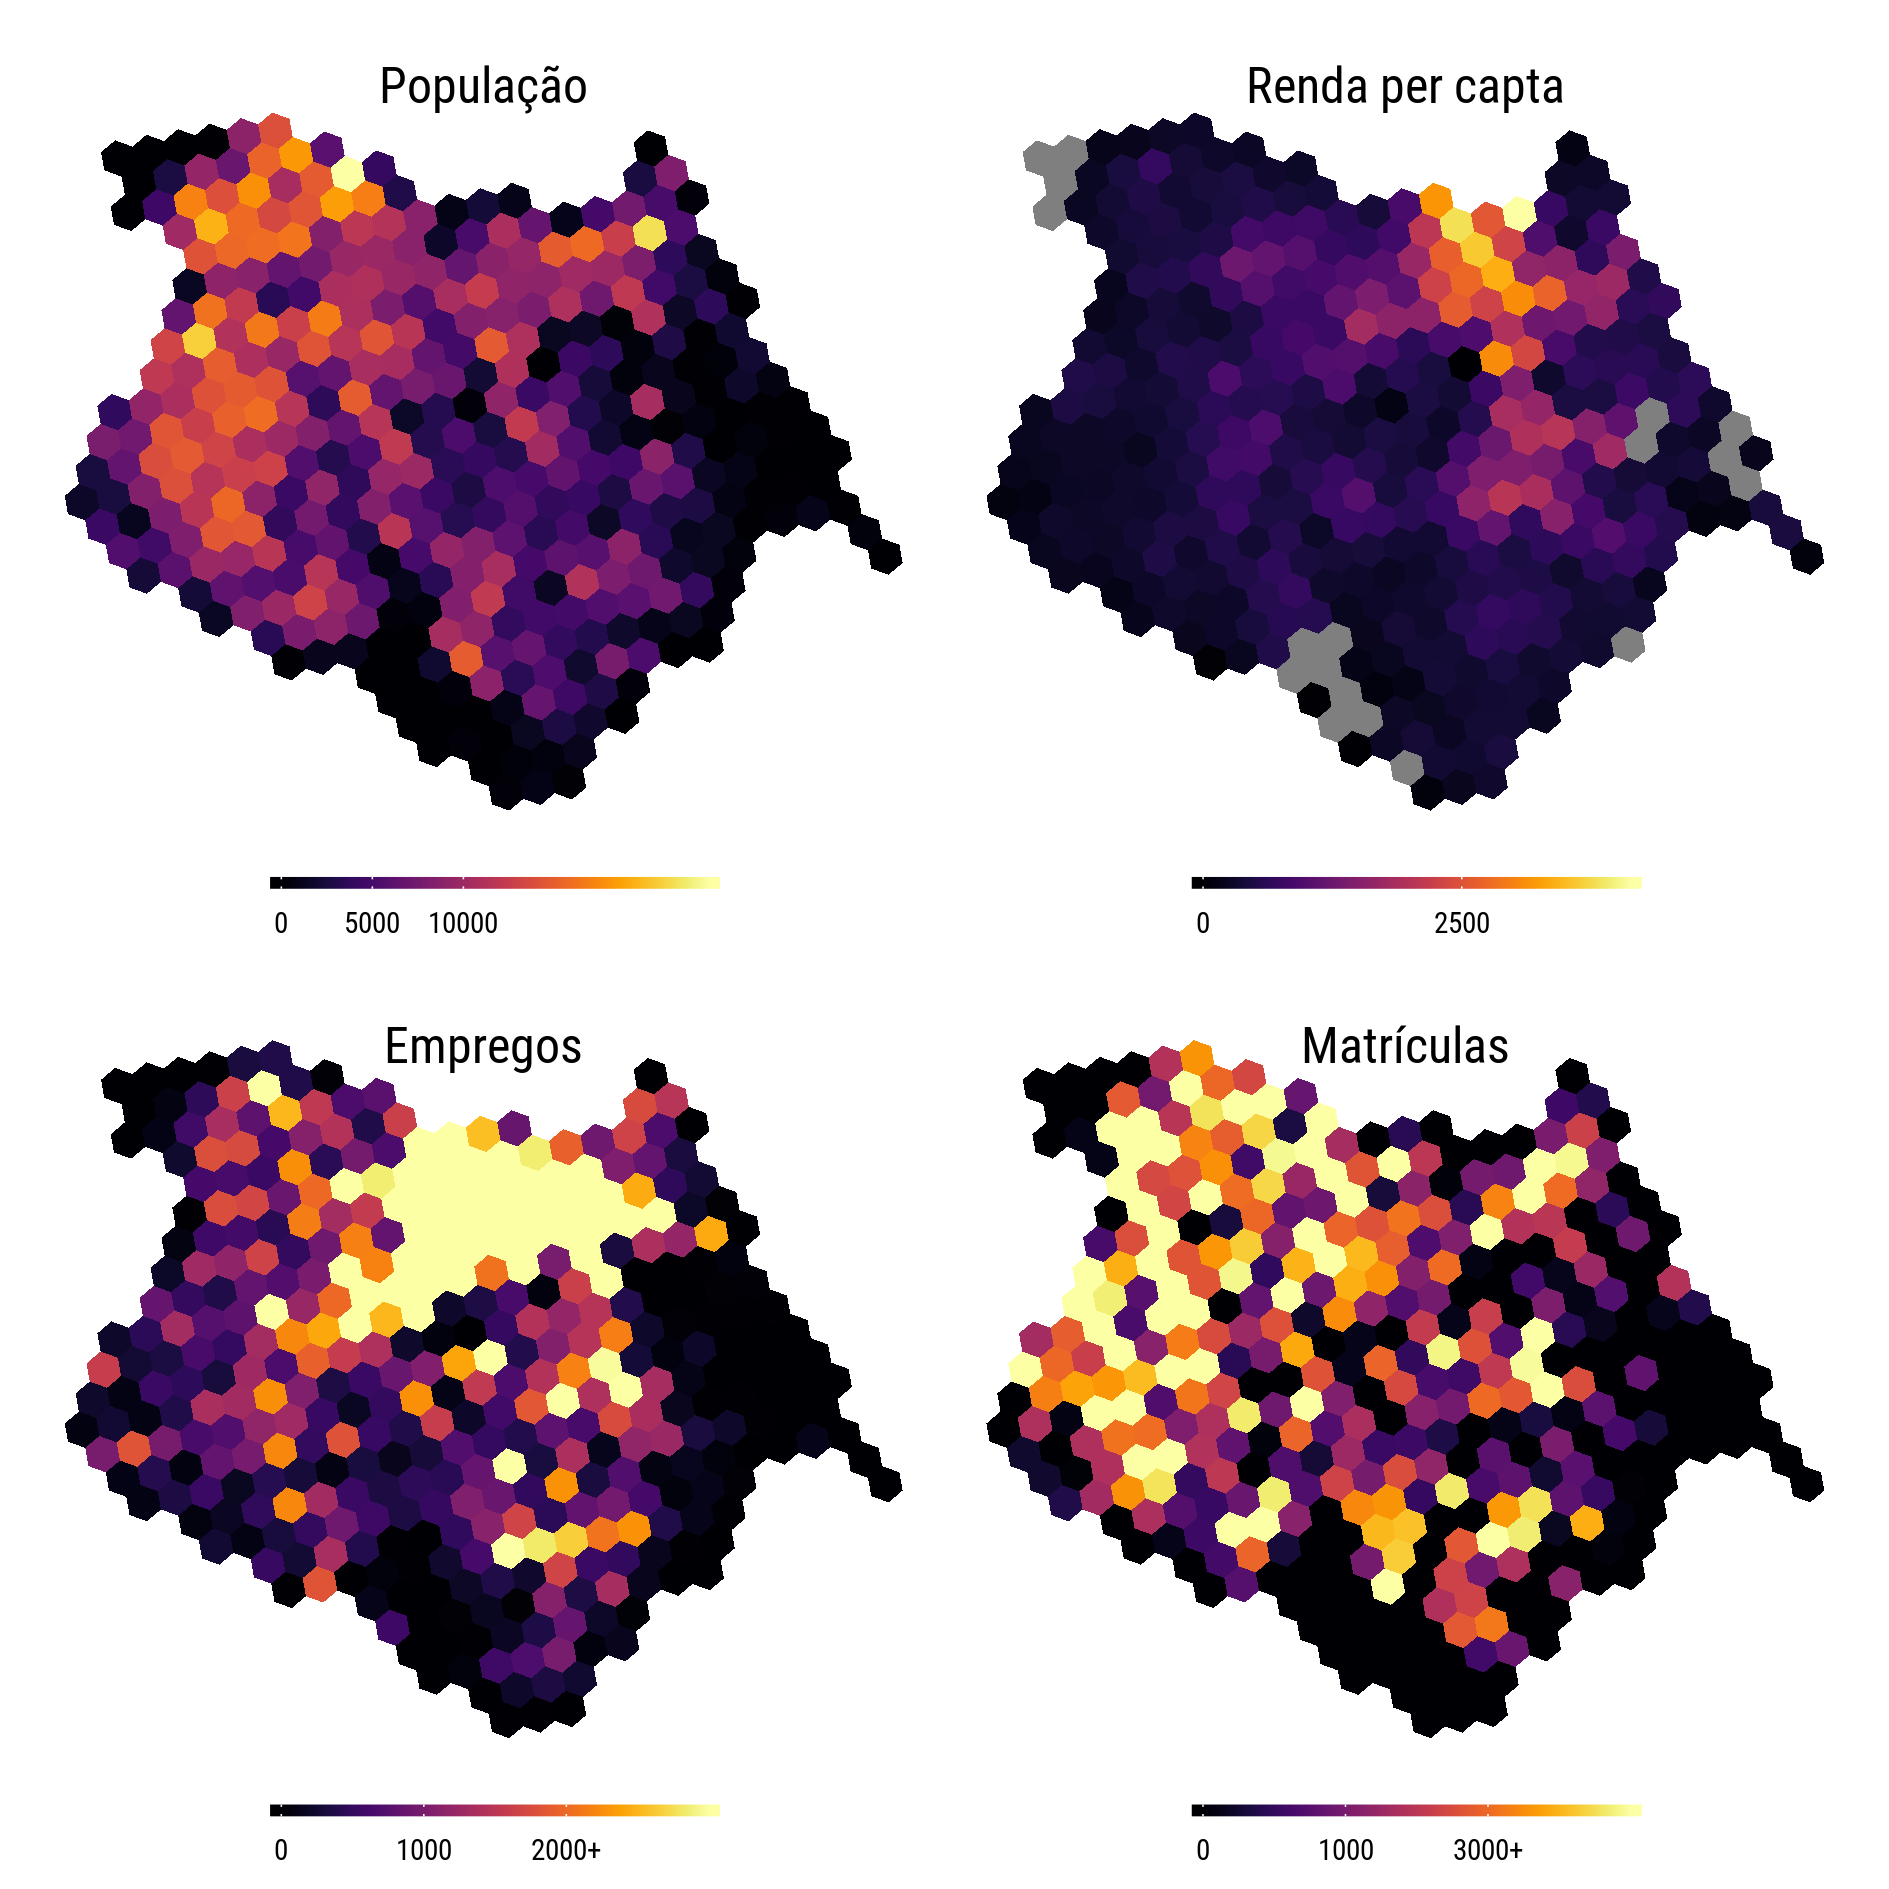
\includegraphics[width=16cm, keepaspectratio]{figure/5-distribuicao_us.png}}
  }{
  \Fonte{Elaborada pelo autor}
  }
  \end{figure}
  
  \hypertarget{calculo-das-matrizes-de-tempo-de-viagem-pelo-otp}{%
  \subsection{Cálculo das matrizes de tempo de viagem pelo OTP}\label{calculo-das-matrizes-de-tempo-de-viagem-pelo-otp}}
  
  Como determinado, foram estimadas matrizes entre todos os pares origem-destino para os horários de 06:45, 07:00, 07:15, 07:30 e 07:45, para o GTFS Programado, o GTFS Empírico P50 e o GTFS Empírico P85. Para unificar esses valores em torno de um valor de tempo de viagem que represente a hora pico, também foi proposto que os tempos de viagem estimados de todos os horários fossem agregados para a sua mediana, separadamente para cada um dos GTFS.
  
  Utilizando os tempos de viagem medianos determinados acima, é feita uma comparação entre o GTFS Programado e o GTFS Empírico P50 (GTFS Corrigido). A Figura \ref{fig:resultado_otp} mostra a distribuição dos tempos de viagem estimados entre os hexágonos, onde o eixo x apresenta os tempos a partir do GTFS Empírico e o eixo y a partir do GTFS Programado. A distribuição da diferença é semelhante à encontrada quando foi feita a comparação com os horários dos ônibus: a maioria dos valores está centrada próximo de uma diferença zero, com uma divisão bem semelhante entre tempos de viagem maiores para o programado (quadrante superior) e maiores para o corrigido (quadrante inferior).
  
  \begin{figure}[!h]
  \captionsetup{width=16cm}
  \Caption{\label{fig:resultado_otp}Densidade do tempo programado x corrigido entre pares origem-destino}
  \centering
  \UFCfig{}{
  {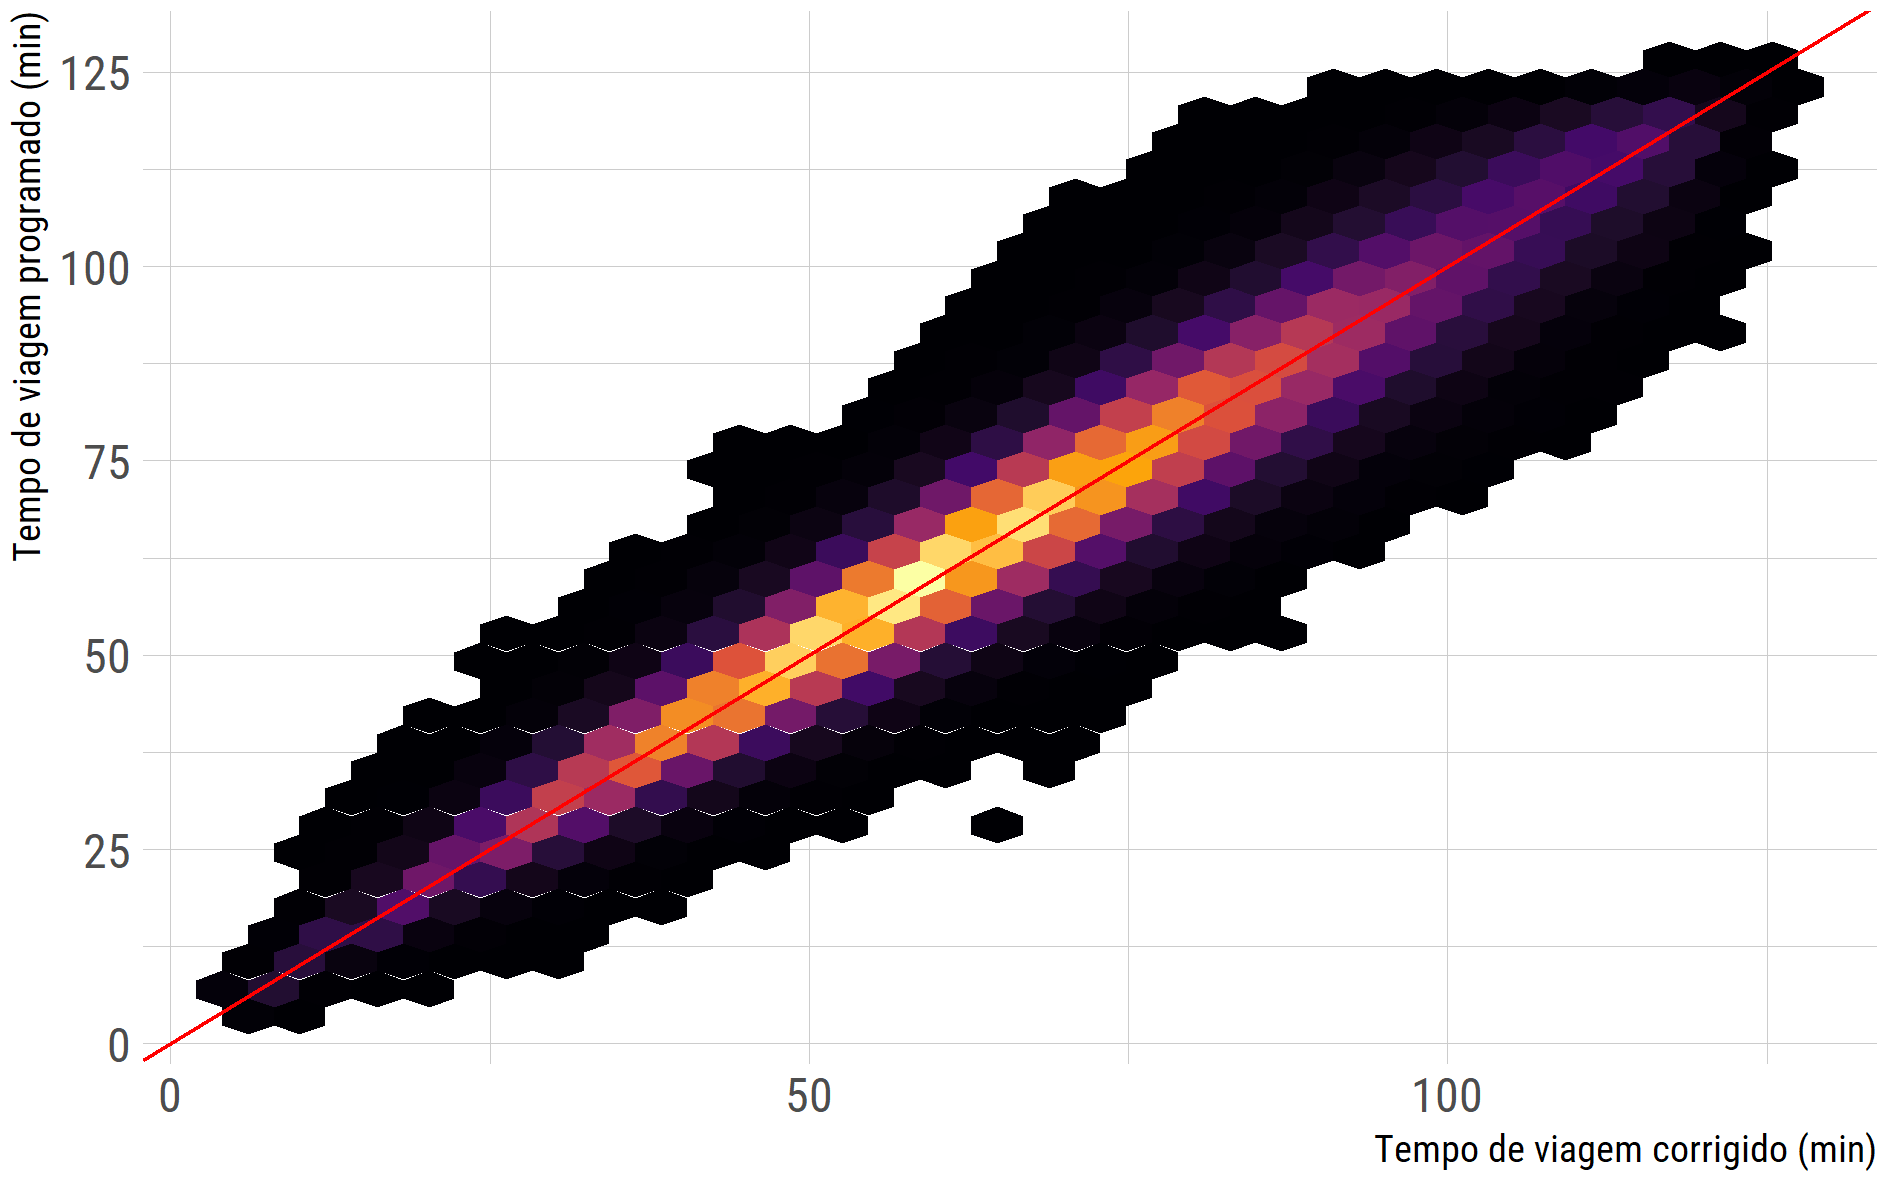
\includegraphics[width=16cm, keepaspectratio]{figure/5-resultado_otp.png}}
  }{
  \Fonte{Elaborada pelo autor}
  }
  \end{figure}
  
  Com as matrizes de tempo de viagem estimadas, parte-se para o cálculo dos indicadores de acessibilidade. Primeiramente, entretanto, é necessário estimar os tempos limites a serem utilizados.
  
  \hypertarget{estimacao-dos-tempos-limite-a-partir-da-bilhetagem}{%
  \subsection{Estimação dos tempos limite a partir da bilhetagem}\label{estimacao-dos-tempos-limite-a-partir-da-bilhetagem}}
  
  A distribuição dos tempos de viagem estimados de cada usuários para os motivos trabalho (utilizaram vale transporte) e educação (utilizaram carteira de estudante) é mostrada na Figura \ref{fig:bi_tt_bp}. No total, foi coletada uma amostra em hora pico de 65 mil viagens para motivo trabalho e 10 mil viagens para motivo educação. Como esperado, a distribuição do tempo de viagem para trabalho tende a valores maiores que para viagens de educação. Como determinado na metodologia, será utilizado o percentil 75 como o tempo limite do indicador respectivo de cada atividade. Pelo gŕáfico, é identificado que esse valor é aproximadamente \textbf{65 minutos} para trabalho e \textbf{50 minutos} para educação.
  
  \begin{figure}[!h]
  \captionsetup{width=16cm}
  \Caption{\label{fig:bi_tt_bp}Distribuição dos tempos de viagem para atividades de trabalho e educação}
  \centering
  \UFCfig{}{
  {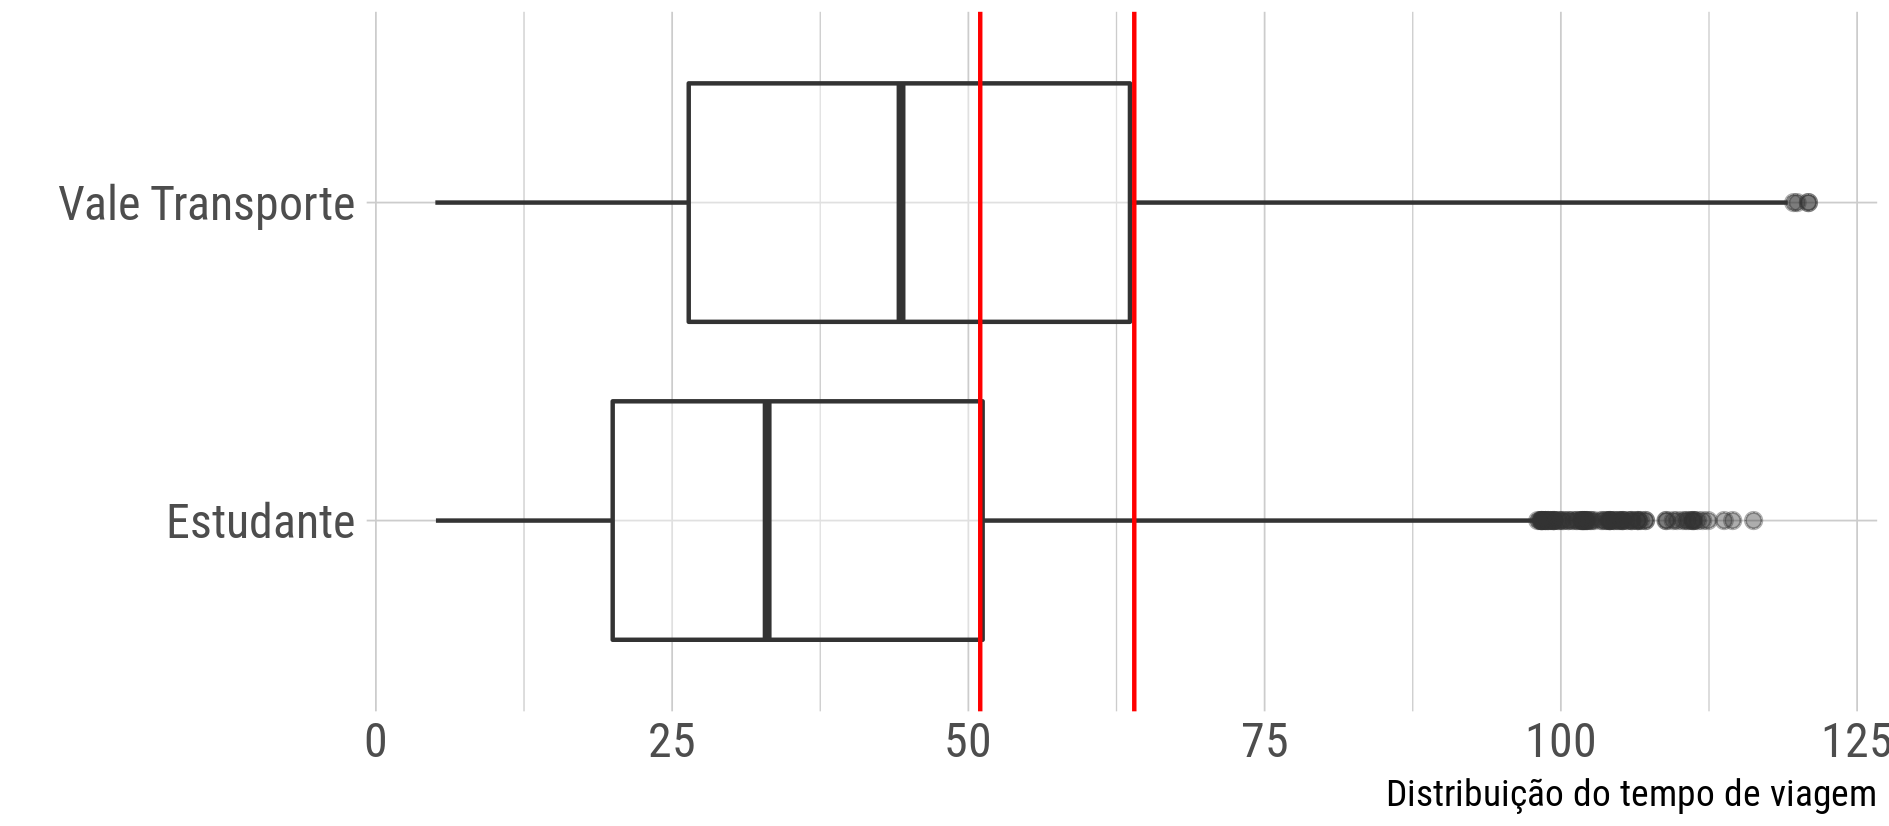
\includegraphics[width=16cm, keepaspectratio]{figure/5-bi_tt_bp.png}}
  }{
  \Fonte{Elaborada pelo autor}
  }
  \end{figure}
  
  As análises da seção anterior trouxeram uma comparação não-espacial dos tempos de viagem estimados tanto pelo GTFS programado como do GTFS corrigido. Agora, é feita a análise incorporando a espacialidade e os dados de uso do solo com o indicador de acessibilidade cumulativa, testando as hipóteses estabelecidas.
  
  \hypertarget{comparacao-da-acessibilidade-para-gtfs-programado-x-gtfs-corrigido}{%
  \section{Comparação da acessibilidade para GTFS Programado x GTFS Corrigido}\label{comparacao-da-acessibilidade-para-gtfs-programado-x-gtfs-corrigido}}
  
  A Figura \ref{fig:h1_tt} abaixo mostra os valores de acessibilidade cumulativa para trabalho em até 65 minutos empírica (P50) x programada, onde cada ponto representa um hexágono. Ao contrário dos tempos de viagem estimado entre pares origem destino, não há uma simetria entre os valores de acessibilidade. A inclusão dos dados de uso do solo na equação mostraram que a acessibilidade para empregos é superestimada pelo GTFS Programado na maioria dos hexaǵonos.
  
  \begin{figure}[!h]
  \captionsetup{width=16cm}
  \Caption{\label{fig:h1_tt}Scatter plot da acessibilidade pelo GTFS Programado x Corrigido para trabalho}
  \centering
  \UFCfig{}{
  {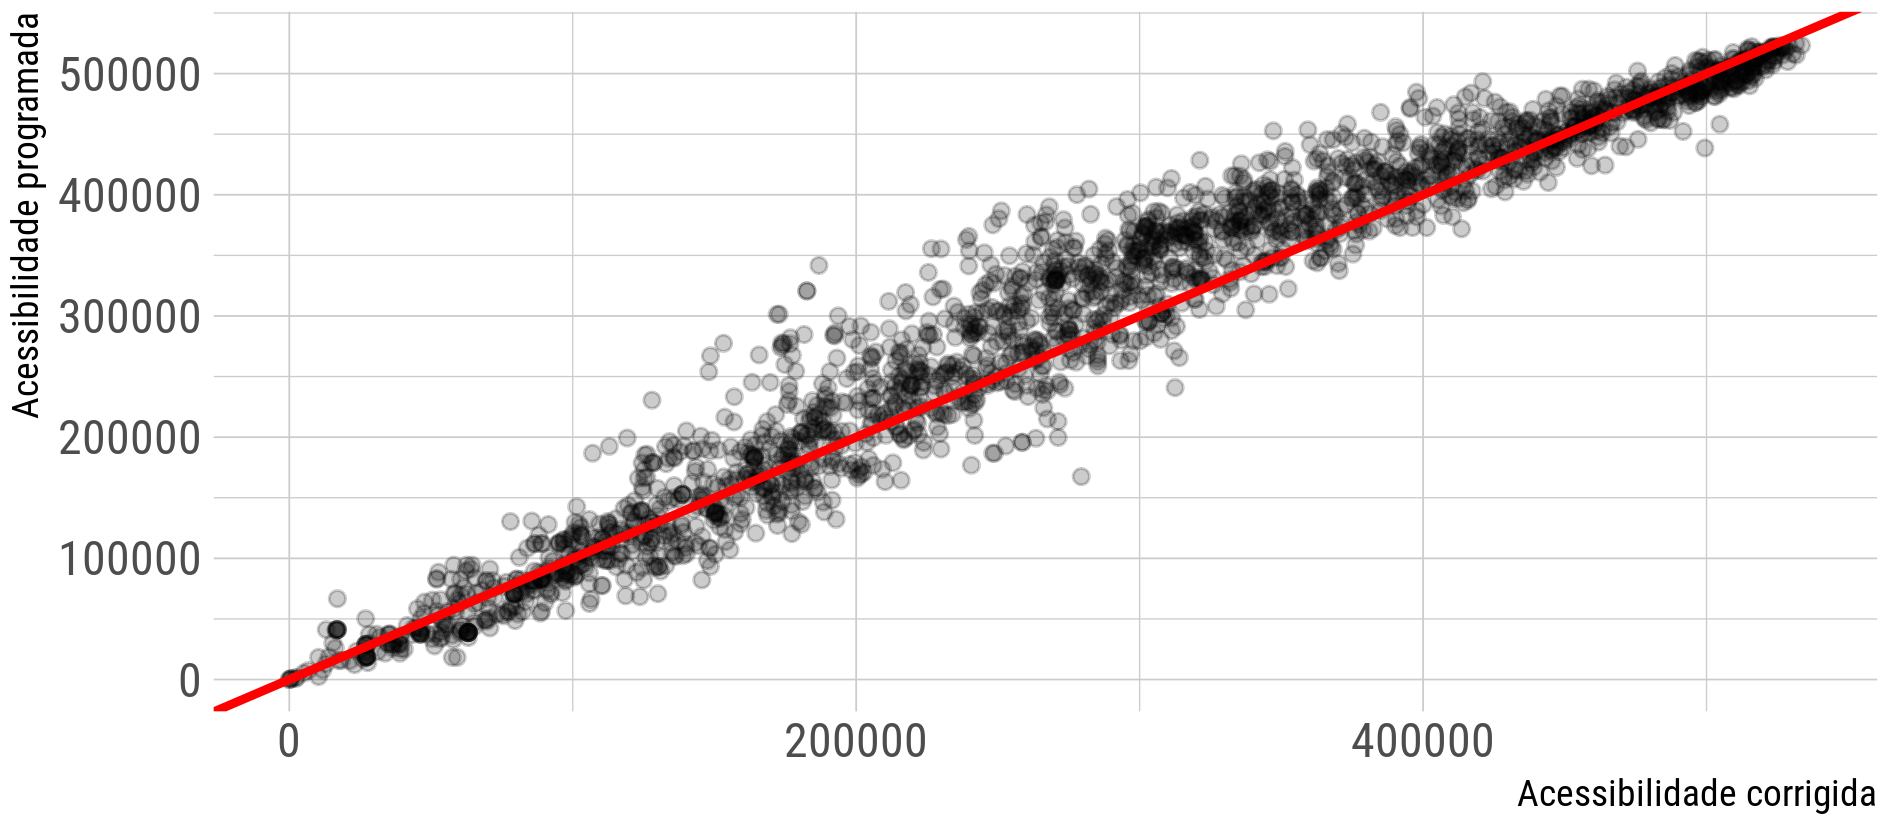
\includegraphics[width=16cm, keepaspectratio]{figure/5-resultado_acess_tt_corrxprogr_sp.png}}
  }{
  \Fonte{Elaborada pelo autor}
  }
  \end{figure}
  
  A Figura \ref{fig:h1_tt_map} espacializa a diferença entre as acessibilidades para motivo trabalho. Valores negativos, em vermelho, indicam onde a acessibilidade pelo GTFS corrigido (P50) foi menor que o GTFS programado. É possível identificar algumas aglomerações tanto de diferenças positivas como de negativas, e essas tendem a se concentrar em regiões periféricas da cidade. Além disso, a diferença de acessibilidade é menor na região da cidade que concentra as atividades de emprego. Mesmo que exista uma diferença entre os horários do GTFS empírico e programado, a acessibilidade tende a não se alterar muito porque, por sua proximidade, o acesso aos hexágonos de maior concentração de atividades continua sendo mantido dentro de um tempo limite de 65 minutos. Para zonas periféricas, entretanto, mesmo uma mudança relativamente pequena no tempo de viagem pode fazer com que estas não alcancem as zonas de maior concentração de atividades - levando a um valor diferente de acessibilidade. A mediana da diferença relativa entre os valores de acessibilidade foi igual a -3,5\%, com um valor do 75º percentil de 2,7\% e do 25º percentil de -14\%.
  
  \begin{figure}[!h]
  \captionsetup{width=16cm}
  \Caption{\label{fig:h1_tt_map}Distribuição espacial da diferença relativa de acessibilidade entre GTFS Programado e Corrigido para trabalho}
  \centering
  \UFCfig{}{
  {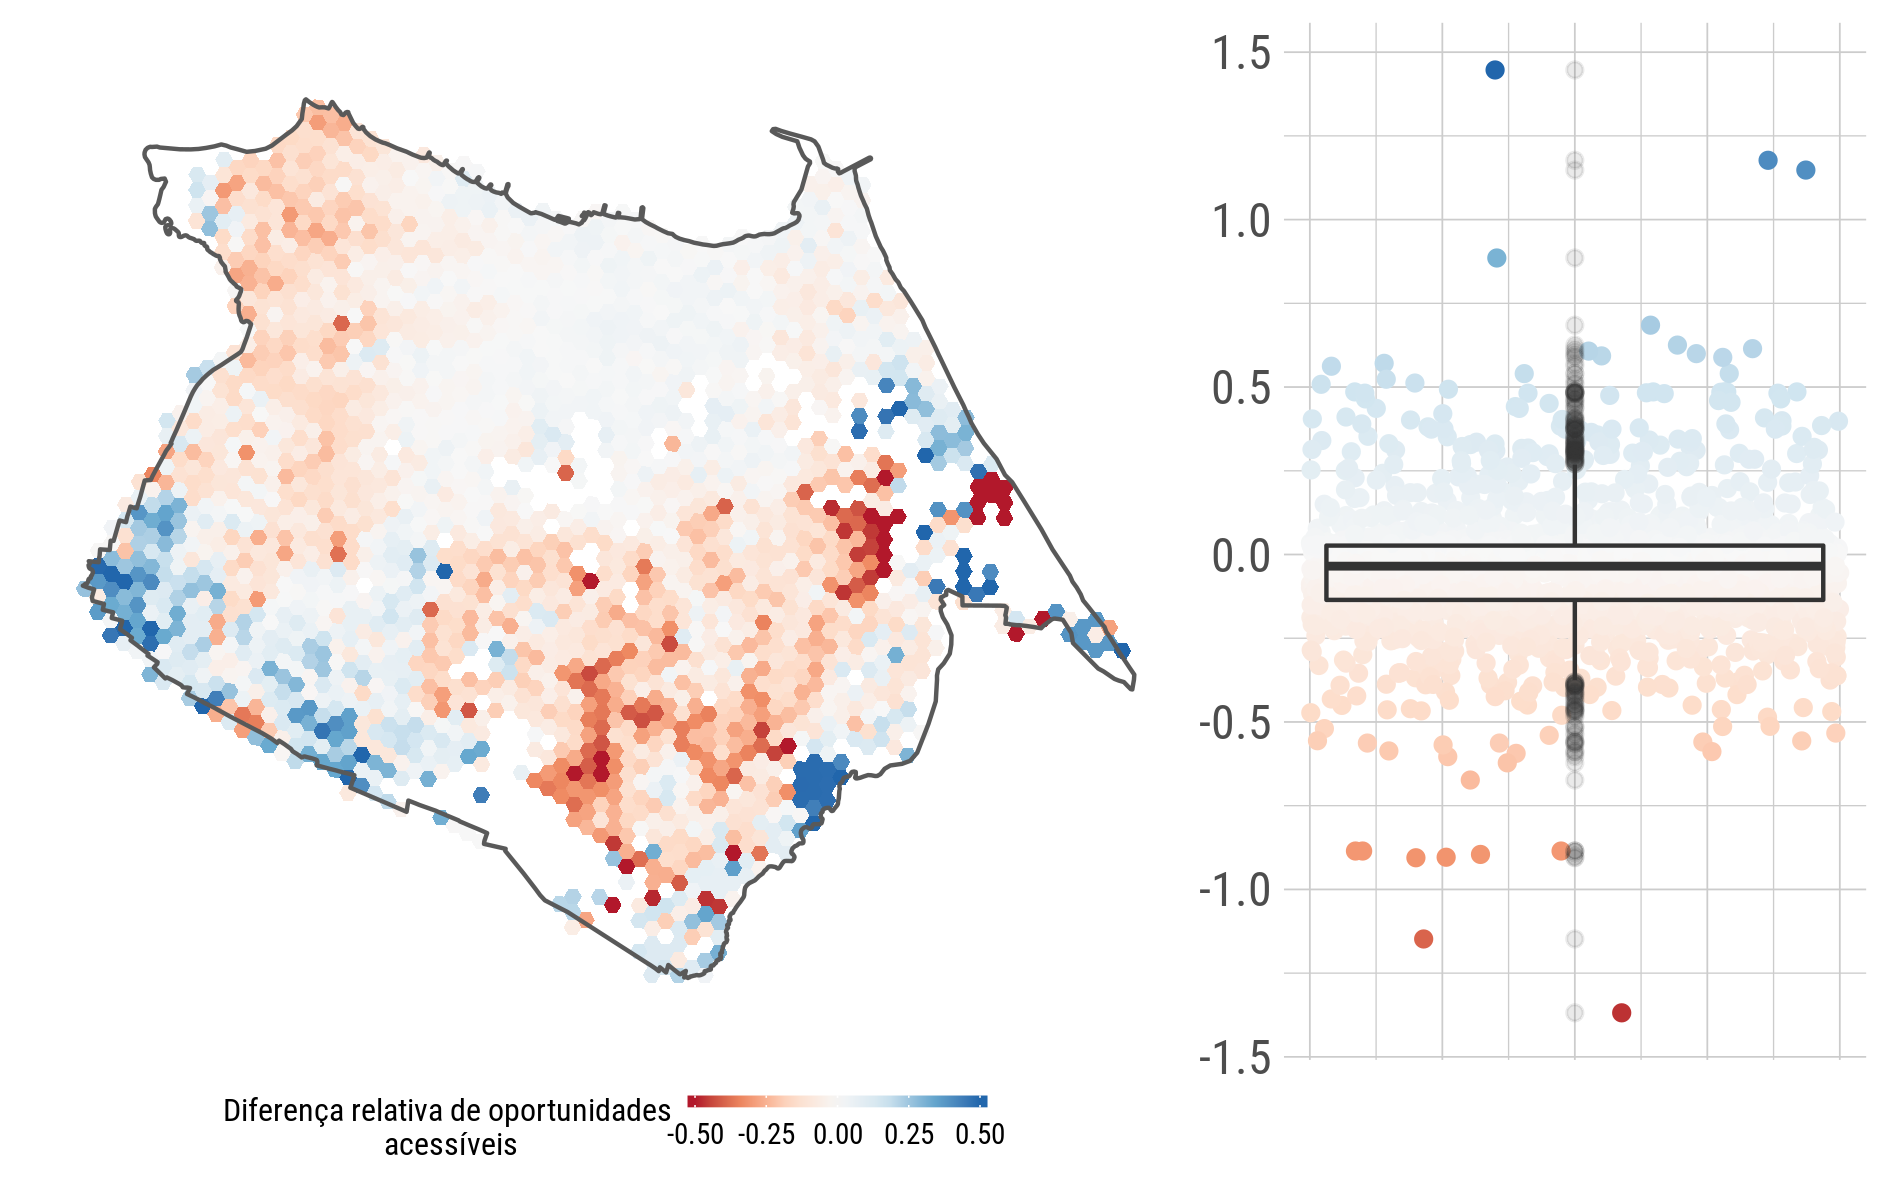
\includegraphics[width=16cm, keepaspectratio]{figure/5-comparacao_gtfs_tt_65.png}}
  }{
  \Fonte{Elaborada pelo autor}
  }
  \end{figure}
  
  A maior parte dos casos críticos de variação relativa encontrados na avaliação da hipótese 1 acontecem em regiões periféricas da cidade, onde a frequência de transporte público tende a ser mais baixa que nas regiões centrais. Isso já era esperado, principalmente em virtude da amostra de tempos de partida coletada (n = 5 horários). Nessas regiões, o tempo de viagem pode variar abruptamente em função da hora que o veículo passa pela área. Por exemplo, se no GTFS padrão o veículo passa 07:20 e no GTFS corrigido o veículo passa 07:02, isso já vai significar uma diferença de 18 minutos no tempo de viagem na matriz de tempo de partida das 07:00 (o primeiro usuário esperaria 20 minutos enquanto o segundo esperaria 2 minutos), sem ainda analisar o tempo dentro do veículo. Apesar da mediana do tempo de viagem de todos os tempos de partida ter sido utilizada, essas zonas ficam mais sujeitas a grande variações de acessibilidade por conta desse fator. Somado a isso, essa diferença de 18 minutos, por exemplo, pode fazer com que um usuário consiga acessar uma parte das zonas de concentração de atividades, enquanto o outro não.
  
  A Figura \ref{fig:h1_et} mostra a acessibilidade corrigida x programada para atividades de educação num tempo limite de 50 minutos. Ao contrário do motivo trabalho, agora os valores tendem a ser mais divididos entre a subestimação e a superestimação, com uma maior tendência à subestimação para valores maiores de acessibilidade. Supõe-se que isso acontece devido à menor concentração de oportunidades dessa atividade na cidade.
  
  \begin{figure}[!h]
  \captionsetup{width=16cm}
  \Caption{\label{fig:h1_et}Scatter plot da acessibilidade pelo GTFS Programado x Corrigido para educação}
  \centering
  \UFCfig{}{
  {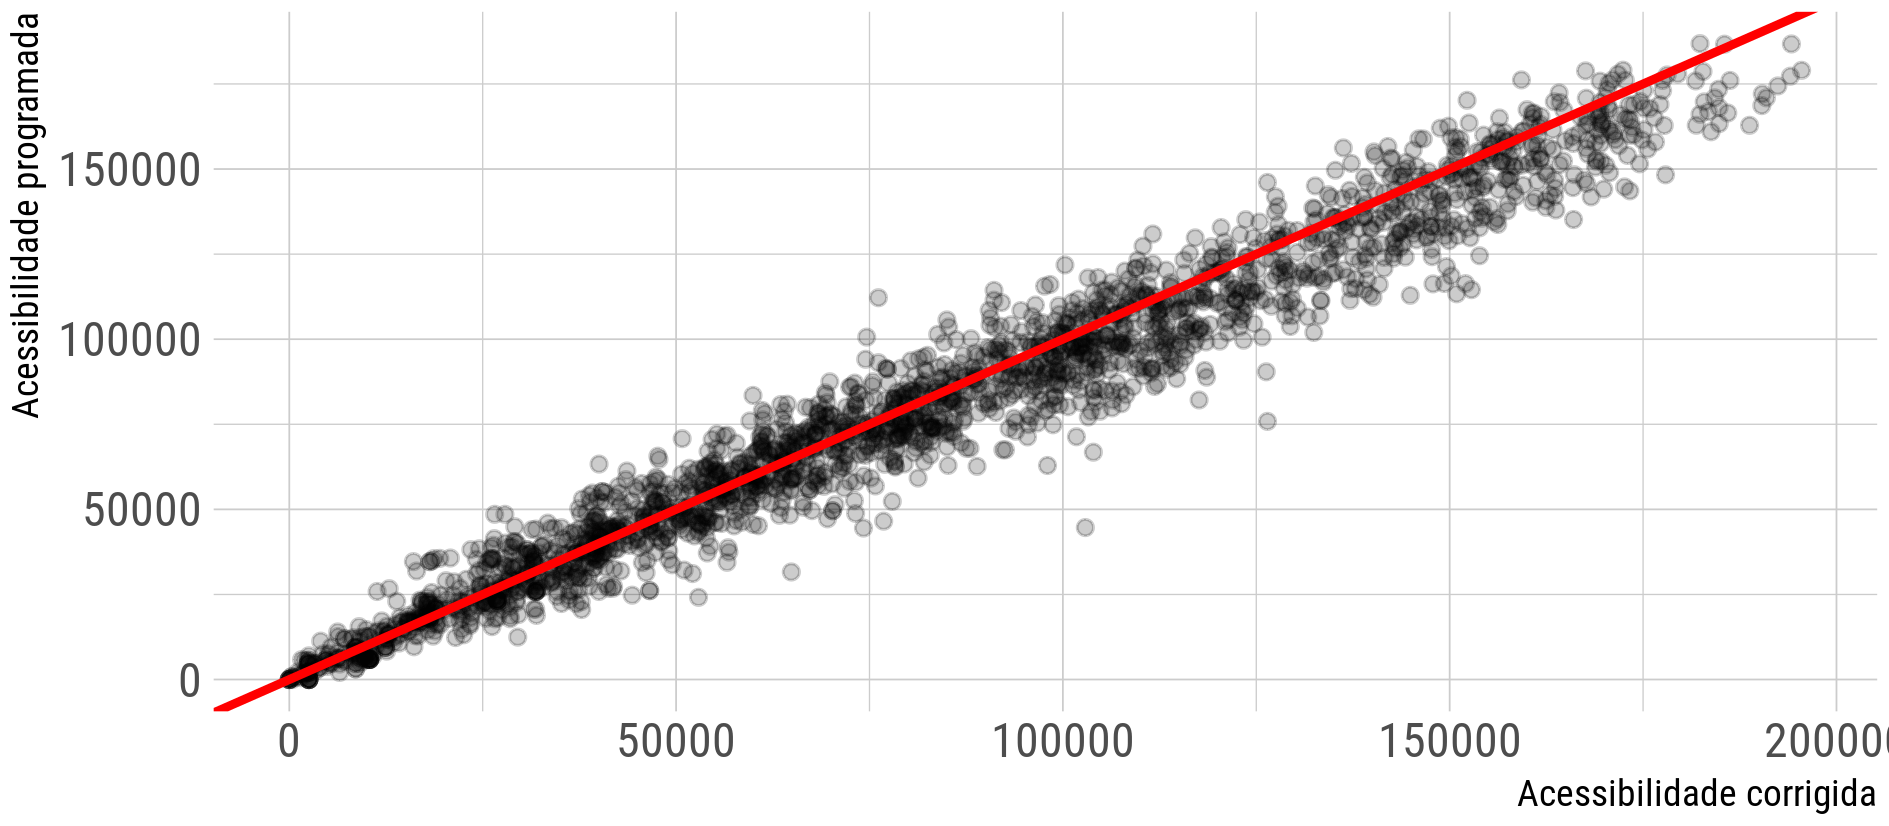
\includegraphics[width=16cm, keepaspectratio]{figure/5-resultado_acess_et_corrxprogr_sp.png}}
  }{
  \Fonte{Elaborada pelo autor}
  }
  \end{figure}
  
  Analisando espacialmente como isso acontece, a Figura \ref{fig:h1_et_map} distribui a diferença relativa (os valores extremos no mapa foram encurtados para +- 50\%). Como observado, a diferença tende a ser menor nas áreas de maior concentração de atividades de educação - no eixo oeste da cidade - pelo mesmo motivo das atividade de trabalho. Valores extremos de diferença continuaram sua tendência de estarem nas bordas. O isolamento espacial somado à baixa frequência de transporte público deixa a acessibilidade dessas zonas muito suscetíveis à variações na chegada e no tempo de deslocamento dos ônibus - que é o que acontece quando é utilizado o GTFS corrigido em vez do programado. A acessibilidade para educação apresenta uma variação menor, com mediana de +3\%, percentil 25 de -5\% e percentil 75 de 12\%.
  
  \begin{figure}[!h]
  \captionsetup{width=16cm}
  \Caption{\label{fig:h1_et_map}Distribuição espacial da diferença relativa de acessibilidade entre GTFS Programado e Corrigido para educação}
  \centering
  \UFCfig{}{
  {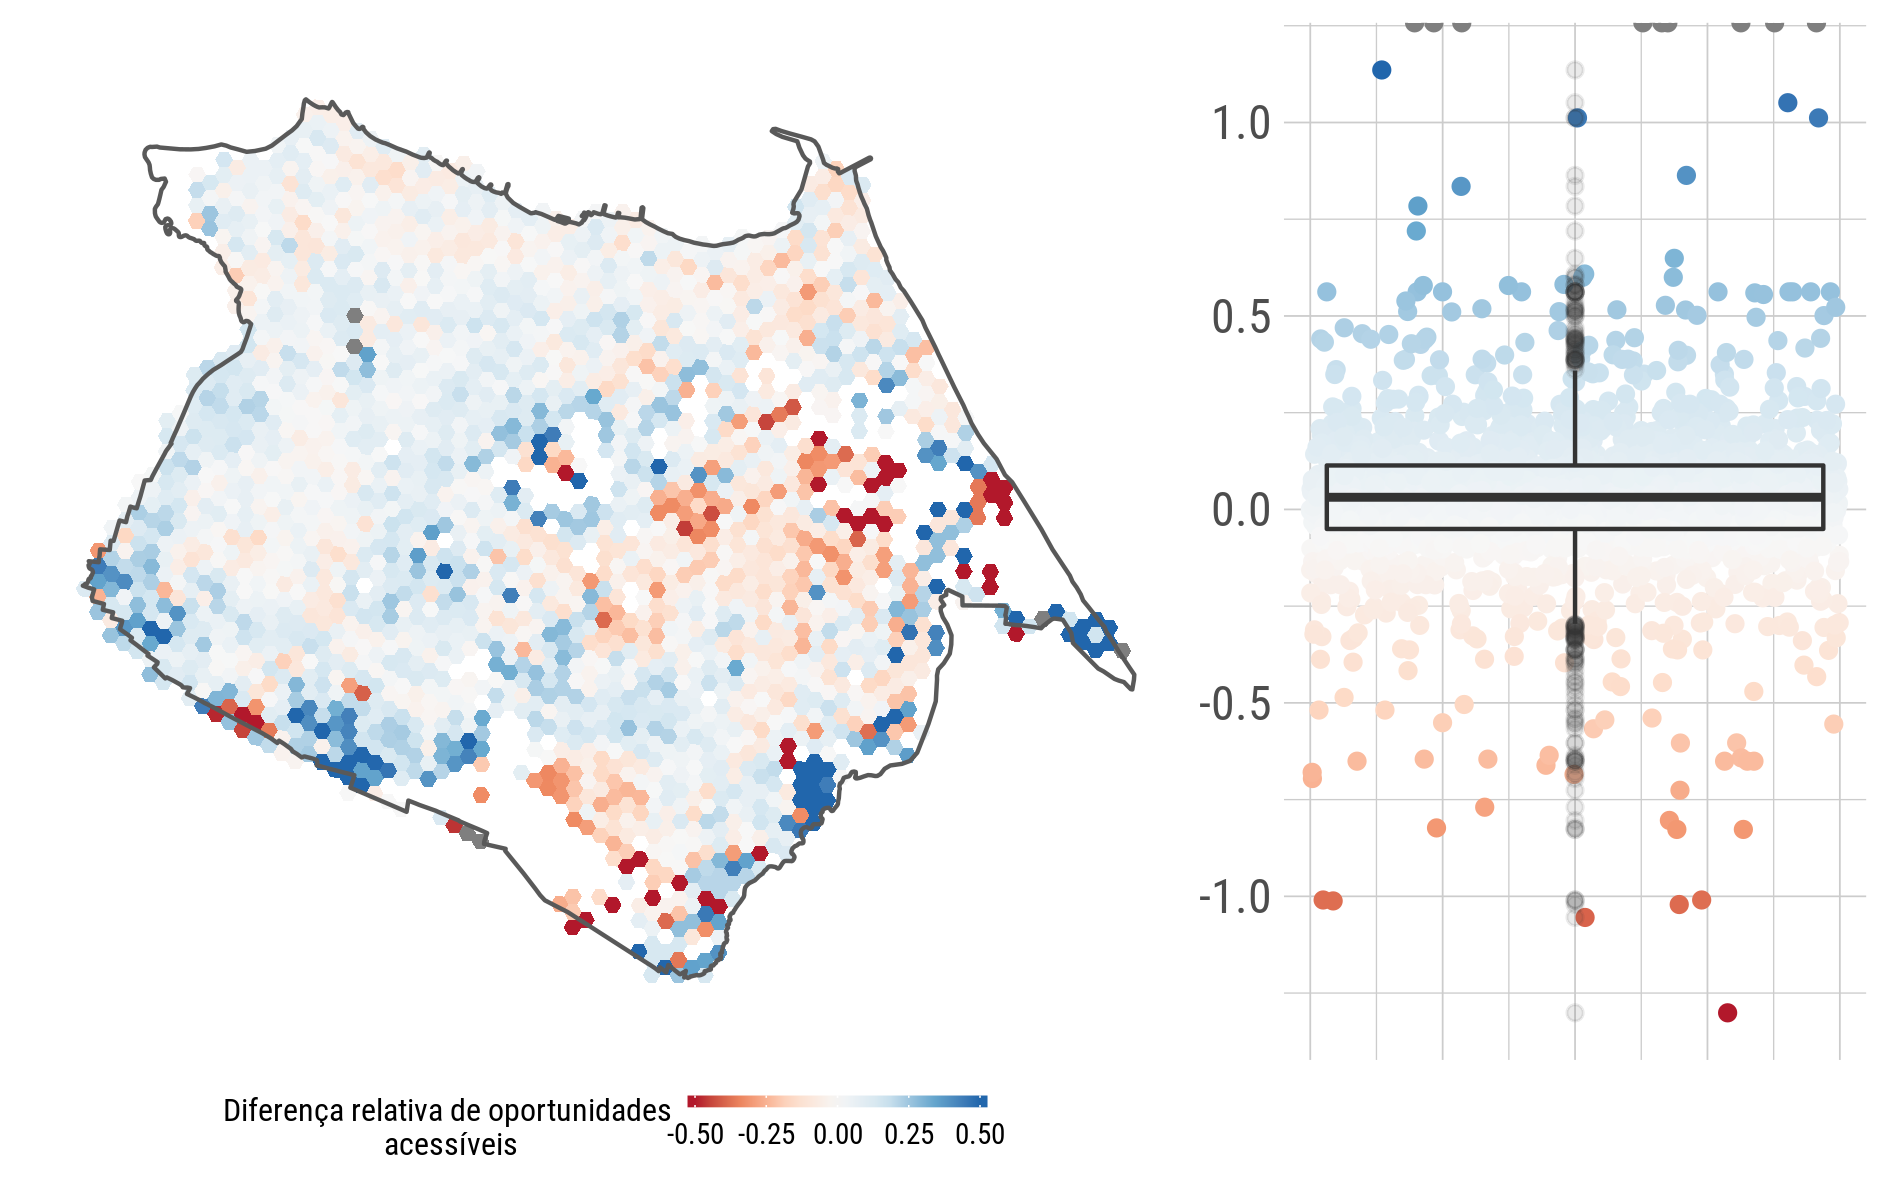
\includegraphics[width=16cm, keepaspectratio]{figure/5-comparacao_gtfs_et_50.png}}
  }{
  \Fonte{Elaborada pelo autor}
  }
  \end{figure}
  
  Os valores relativos apresentados acima podem não ser impactantes o suficiente para mostrar a diferença que a acessibilidade pode ter entre os dois tipos de dados. Para isso, a Figura \ref{fig:h1_abs} mostra a distribuição dos valores de diferença absoluta para trabalho (esquerda) e educação (direita). É possível ver as tendências opostas. Um exemplo: análises utilizando GTFS programado tendem a superestimar em até mais de 100 mil empregos a acessibilidade para algumas regiões no sul da cidade (aglomerações em vermelho no mapa). Para trabalho, o valor do percentil 25 é de -37 mil, com mediana de -9 mil e percentil 75 de +7,5 mil empregos. Para educação, os valores são -3 mil, +2 mil e +8,5 mil, respectivamente.
  
  A parte inferior da Figura \ref{fig:h1_abs} mostra a diferença absoluta de acessibilidade na forma da porcentagem do total de atividades. Ela é calculada fazendo a divisão da diferença absoluta pela quantidade de atividades total na cidade de trabalho ou educação, permitindo que seja feita uma comparação da distribuição entre as duas atividades. É observado que a dispersão é maior para atividades de trabalho, onde em média o GTFS Programado superestima a acessibilidade em 3\% do total de empregos da cidade. Para educação, o GTFS Programado subestima a acessibilidade 1\% do total de matrículas.
  
  \begin{figure}[!h]
  \captionsetup{width=16cm}
  \Caption{\label{fig:h1_abs}Distribuição da diferença absoluta de acessibilidade entre GTFS Programado e Corrigido para trabalho (esquerda) e educação (direita)}
  \centering
  \UFCfig{}{
  {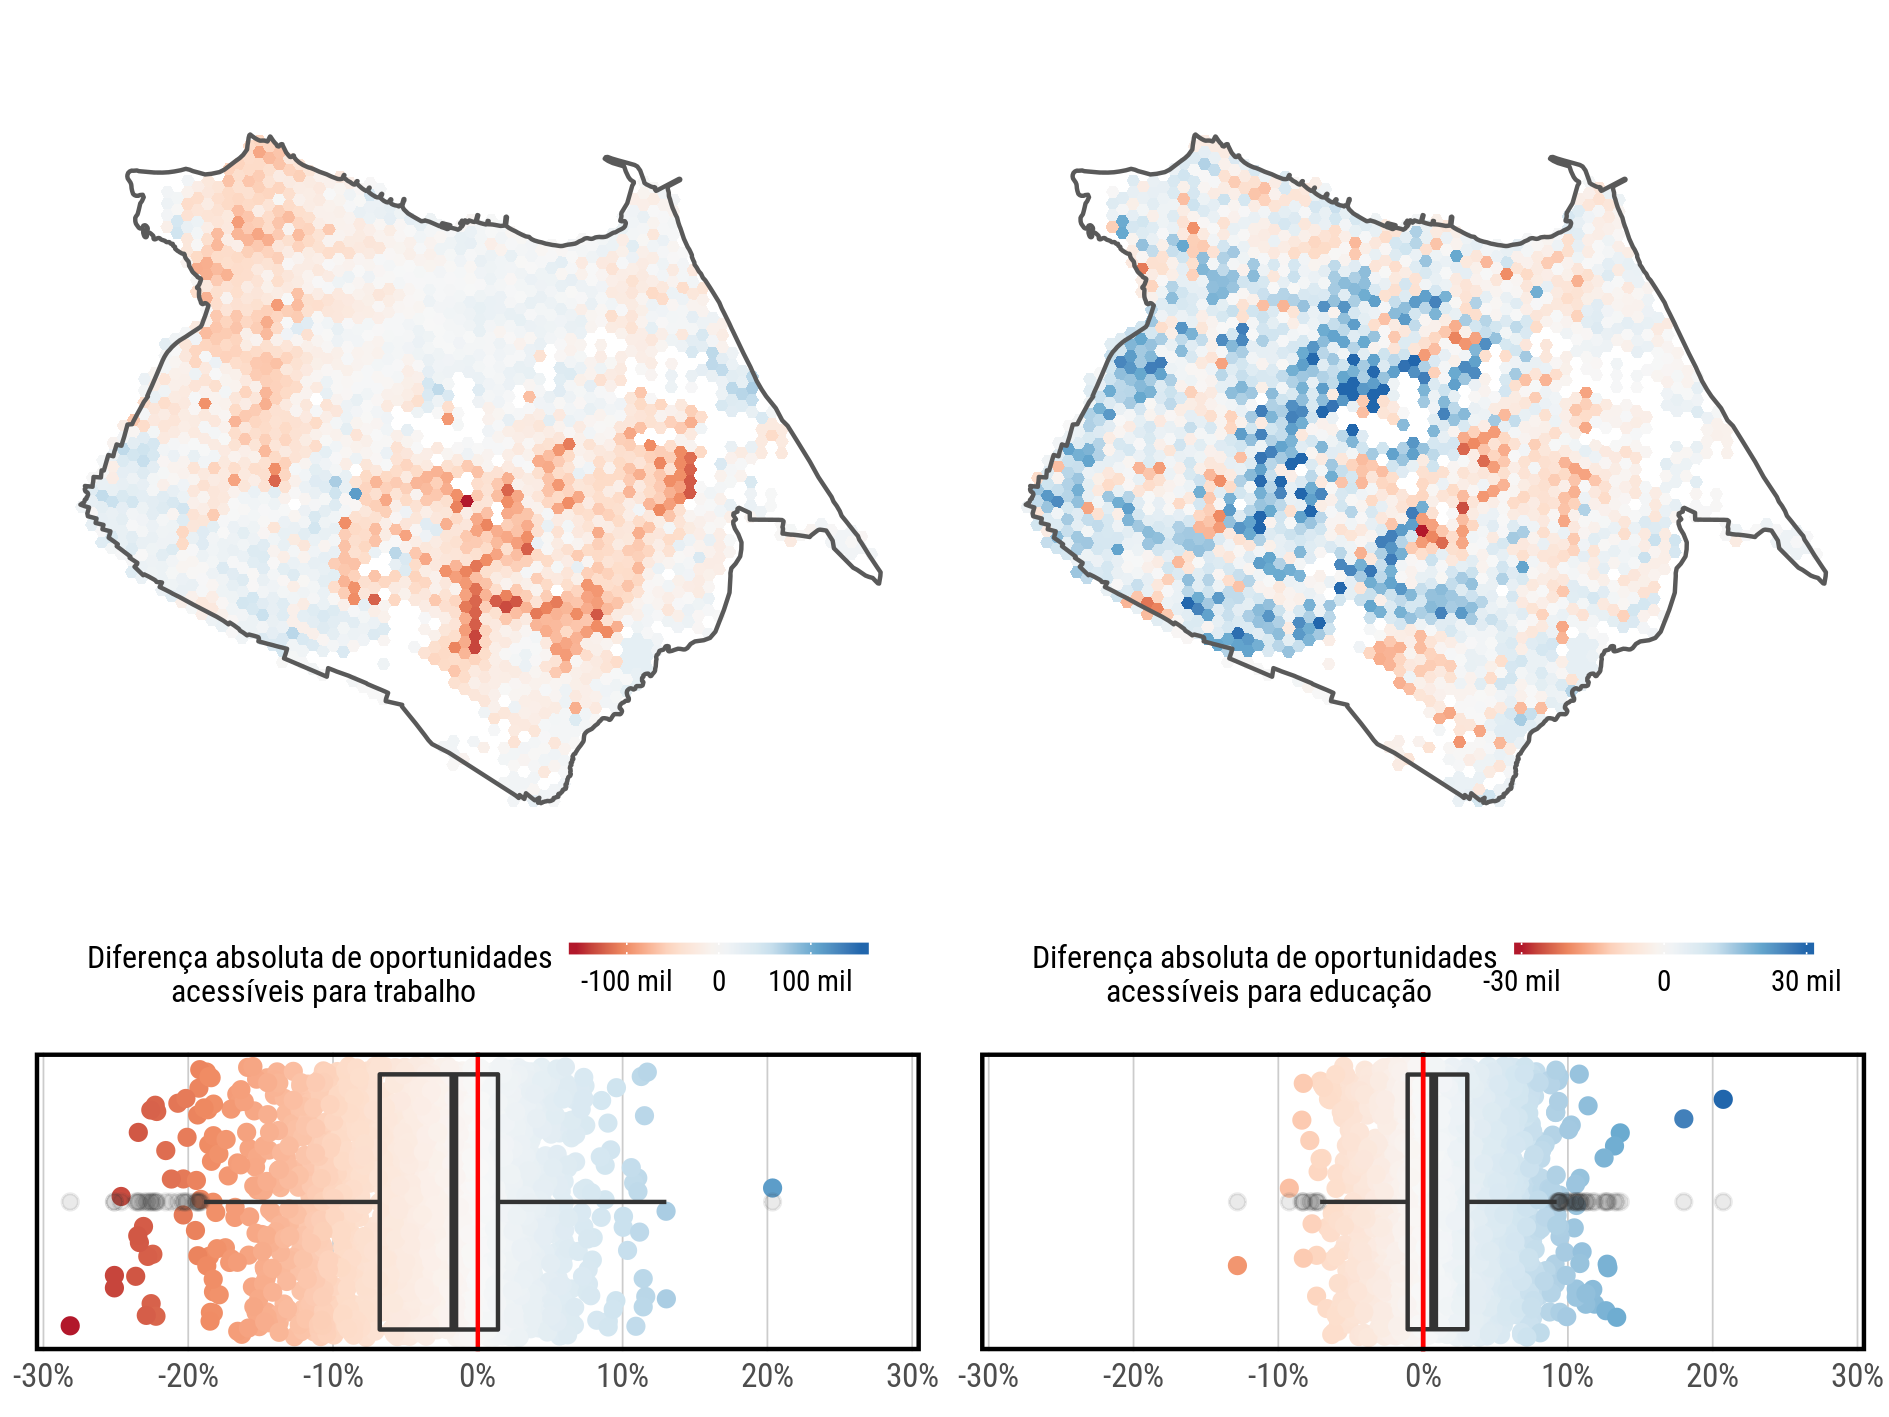
\includegraphics[width=16cm, keepaspectratio]{figure/5-comparacao_gtfs_absoluto.png}}
  }{
  \Fonte{Elaborada pelo autor}
  }
  \end{figure}
  
  Para a análise espacial da diferença absoluta para empregos, é observado que zonas com alta diferença de acessibilidade estão presentes nas ``bordas'' de entrada da zona de concentração de atividades (centro da cidade). Isso indica que o GTFS Programado falha ao captar prováveis condições de congestionamento nas vias (captadas pelo GTFS Corrigido) que levam os usuários da periferia para o centro da cidade.
  
  Para educação, o padrão identificado é diferente. Essas atividades têm uma dispersão maior na cidade, com uma leve concentração na região oeste da cidade. Isso significa que o acesso à essas zonas está menos sujeito à congestionamentos e atrasos dos veículos, levando a uma maior pontualidade dos horários programados, o que por fim leva a uma menor variação da acessibilidade. A variação absoluta foi até positiva na maioria dos casos, sugerindo que os horários programados em fluxos no sentido de pouco congestionamento podem ser conservadores.
  
  Para mostrar como essa grande diferença de acessibilidade acontece, foi selecionado um hexágono crítico de acessibilidade e feito a comparação da sua área de influência (a quantidade de hexágonos que aquele hexágono consegue acessar para o tempo limite de 65 minutos), para os dois cenários, para a acessibilidade para emprego. A Figura \ref{fig:h1_extremo} mostra a área de influência de um hexágono em uma zona urbanizada da cidade que teve uma diferença de aproximadamente 90 mil empregos entre os dois cenários. A área de influência em azul apresenta as zonas acessíveis a partir do GTFS programado, enquanto a área em vermelho a partir do GTFS P50 (a área em vermelho mais escuro apresenta as zonas que são acessíveis para os dois casos). É observado que a utilização dos horários de viagem corrigidos leva o morador daquele hexágono a acessar menos zonas do centro da cidade. Isso, somado à grande concentração de emprego nessas zonas agora não acessíveis, faz com que o usuário tenha essa diferença de acesso. O fato da área de influência chegar a regiões do extremo leste e oeste da cidade (vermelho mais claro) acaba não fazendo uma grande diferença porque essas regiões não apresentam grande quantidade de empregos.
  
  \begin{figure}[!h]
  \captionsetup{width=16cm}
  \Caption{\label{fig:h1_extremo}Áreas de influência do GTFS Programado (azul) e do GTFS Corrigido (vermelho) de zona crítica}
  \centering
  \UFCfig{}{
  {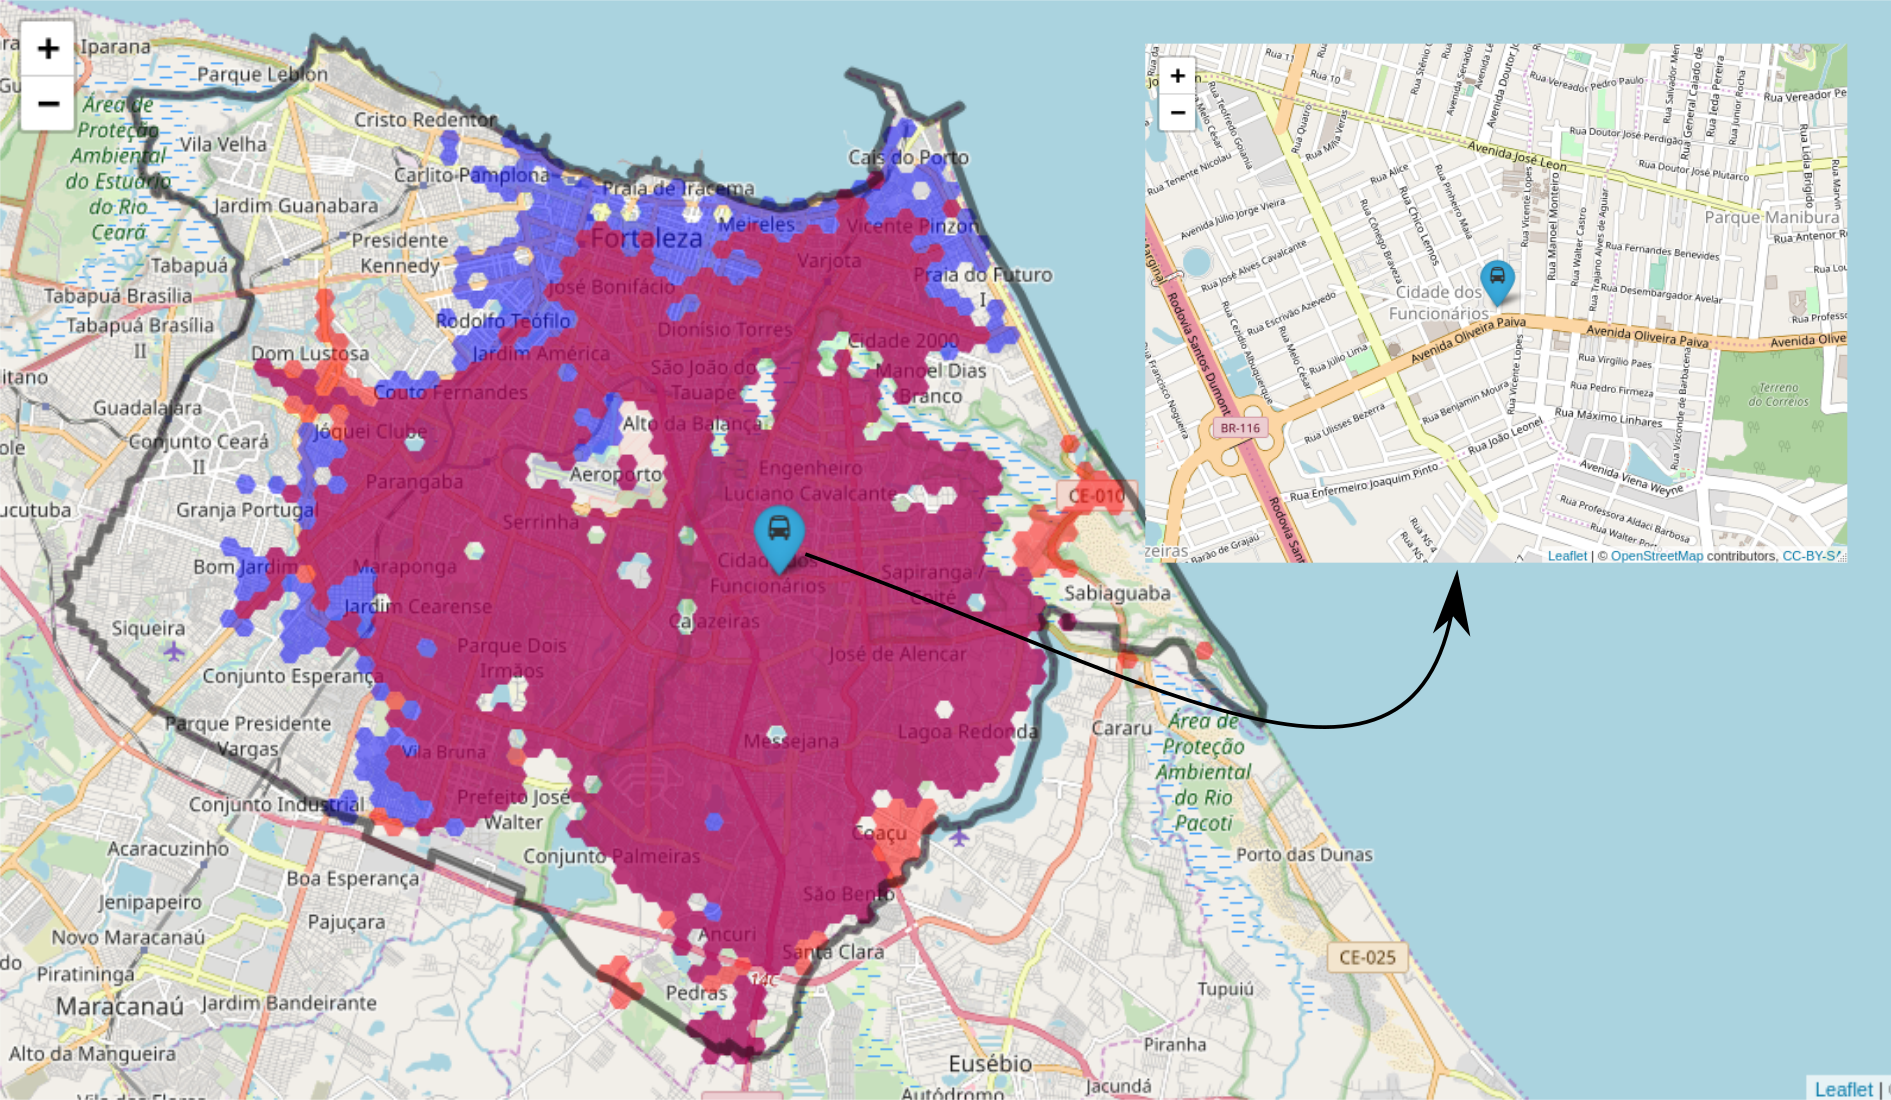
\includegraphics[width=16cm, keepaspectratio]{figure/5-acess_extremo_padraoxp50_fim.png}}
  }{
  \Fonte{Elaborada pelo autor}
  }
  \end{figure}
  
  Os resultados também confirmam uma limitação que foi levantada no capítulo anterior: a do tamanho da amostra de horas de partida. Para a maioria das localidades, especialmente as zonas mais centrais, que tem uma boa frequência de serviço, é entendido que essa amostra a cada 15 minutos satisfaz. Porém, essa limitação é mais clara na análise da diferença relativa de acessibilidade entre os cenários da hipótese 1, para as zonas mais periféricas. Uma amostra maior (a cada 5 minutos, por exemplo) tenderia a suavizar e consolidar os valores de variação para as zonas mais distantes (que têm uma menor frequência de transporte público).
  
  É possível analisar como a utilização de dados empíricos da frota poderia impactar a tomada de decisões em intervenções no sistema de transporte. Como observado, para trabalho, dados de GTFS Programado tendem a superestimar a acessibilidade em zonas de entrada do centro da cidade em até 100 mil empregos. Intervenções e análises a partir desses dados tenderiam a superestimar esses valores, podendo levar à decisões de intervenções equivocadas. Um exemplo que pode ser dado é sobre a questão de intervir construindo um corredor misto de transporte em vez de um corredor exclusivo de ônibus. Num contexto de horários programados, uma análise \emph{ex-post} poderia concluir que houve ganhos de acessibilidade bem semelhantes entre as alternativas, visto que os horários programados tendem a não incorporar informações de \emph{bus bunching} e consequentes atrasos. Quando horários empíricos são incorporados, a diferença entre um cenário de tráfego misto e tráfego exclusivo só de ônibus tende a ser incorporada de forma mais correta.
  
  \hypertarget{comparacao-da-acessibilidade-para-gtfs-p50-x-gtfs-p85}{%
  \section{Comparação da acessibilidade para GTFS P50 x GTFS P85}\label{comparacao-da-acessibilidade-para-gtfs-p50-x-gtfs-p85}}
  
  É feita a comparação da acessibilidade para os dois cenários de tempo de viagem estabelecidos: o tempo da mediana (P50) e o tempo do percentil 85 (P85). A Figura \ref{fig:h2} espacializa os dois indicadores para atividades de emprego e educação para uma mesma escala de cores, buscando mostrar visualmente as diferenças. É notório que há uma abrangência mais clara e maior do indicador utilizando os tempos de viagem medianos (P50), com os corredores de alta acessibilidade mais claros e definidos. Esses corredores variam entre as atividades, estando localizados mais em direção ao centro para as atividades de empregos e mais para centro e oeste para as atividades de educação. Zonas do extremo sul e do extremo leste da cidade aparentam não mudarem muito sua acessibilidade.
  
  \begin{figure}[!h]
  \captionsetup{width=16cm}
  \Caption{\label{fig:h2}Indicador cumulativo de oportunidades para GTFS Empírico P50 (esquerda) e P85 (direita) para trabalho}
  \centering
  \UFCfig{}{
  {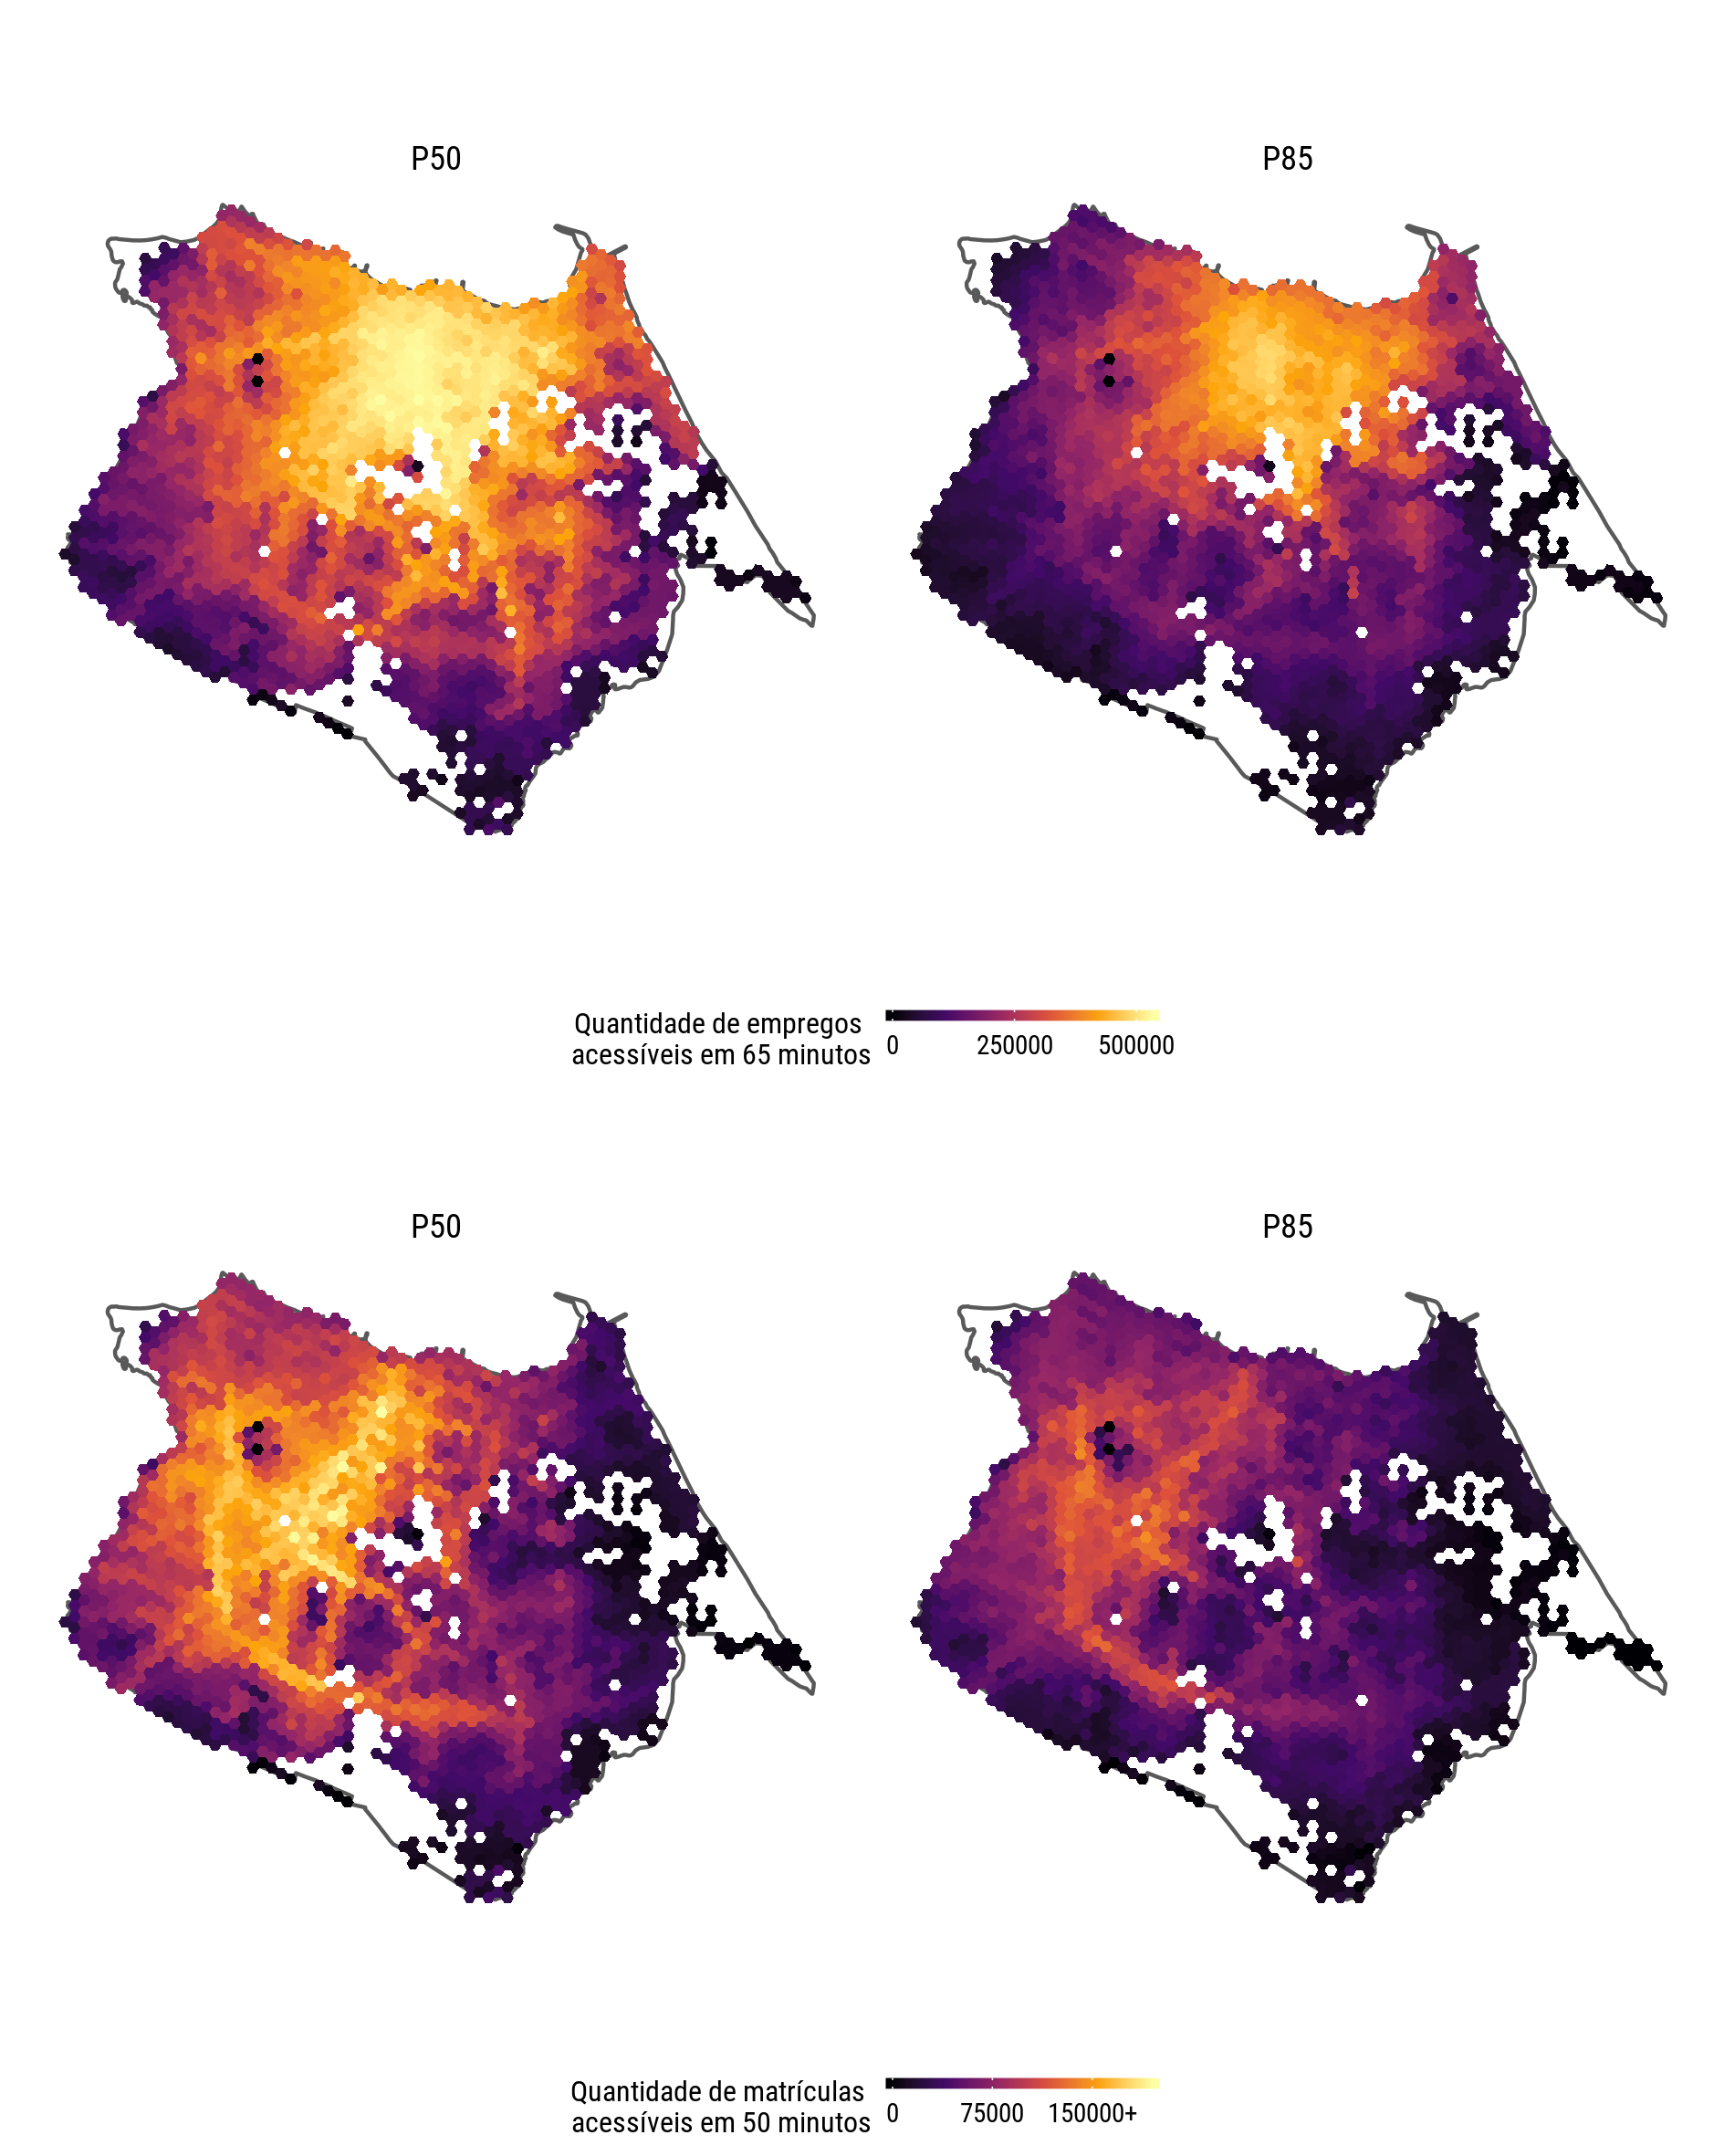
\includegraphics[width=16cm, keepaspectratio]{figure/5-acess_cenarios.png}}
  }{
  \Fonte{Elaborada pelo autor}
  }
  \end{figure}
  
  Para identificar as zonas que mais sofrem com a variabilidade dos tempos de viagem, a Figura \ref{fig:h2_abs} mostra a cidade com as diferenças absolutas de acessibilidade entre os cenários para empregos (esquerda) e matrículas (direita). É notado, principalmente, que há uma aglomeração a sul do centro geográfico da cidade para trabalho. Assume-se que essa aglomeração seja em virtude da alta variabilidade de tempo de viagem encontrada na região próxima a BR-116, onde há um encontro do fluxo advindo das regiões centro-sul e sudoeste na cidade. Nessas regiões, a variabilidade pode causar uma diferença de até 200000 empregos acessíveis. O número, que pode parecer excessivo, acontece porque a imprevisibilidade pode levar o usuário a deixar de acessar as zonas de aglomeração de atividades da cidade.
  
  \begin{figure}[!h]
  \captionsetup{width=16cm}
  \Caption{\label{fig:h2_abs}Diferença absoluta de acessibilidade entre cenários para trabalho (esquerda) e educação (direita)}
  \centering
  \UFCfig{}{
  {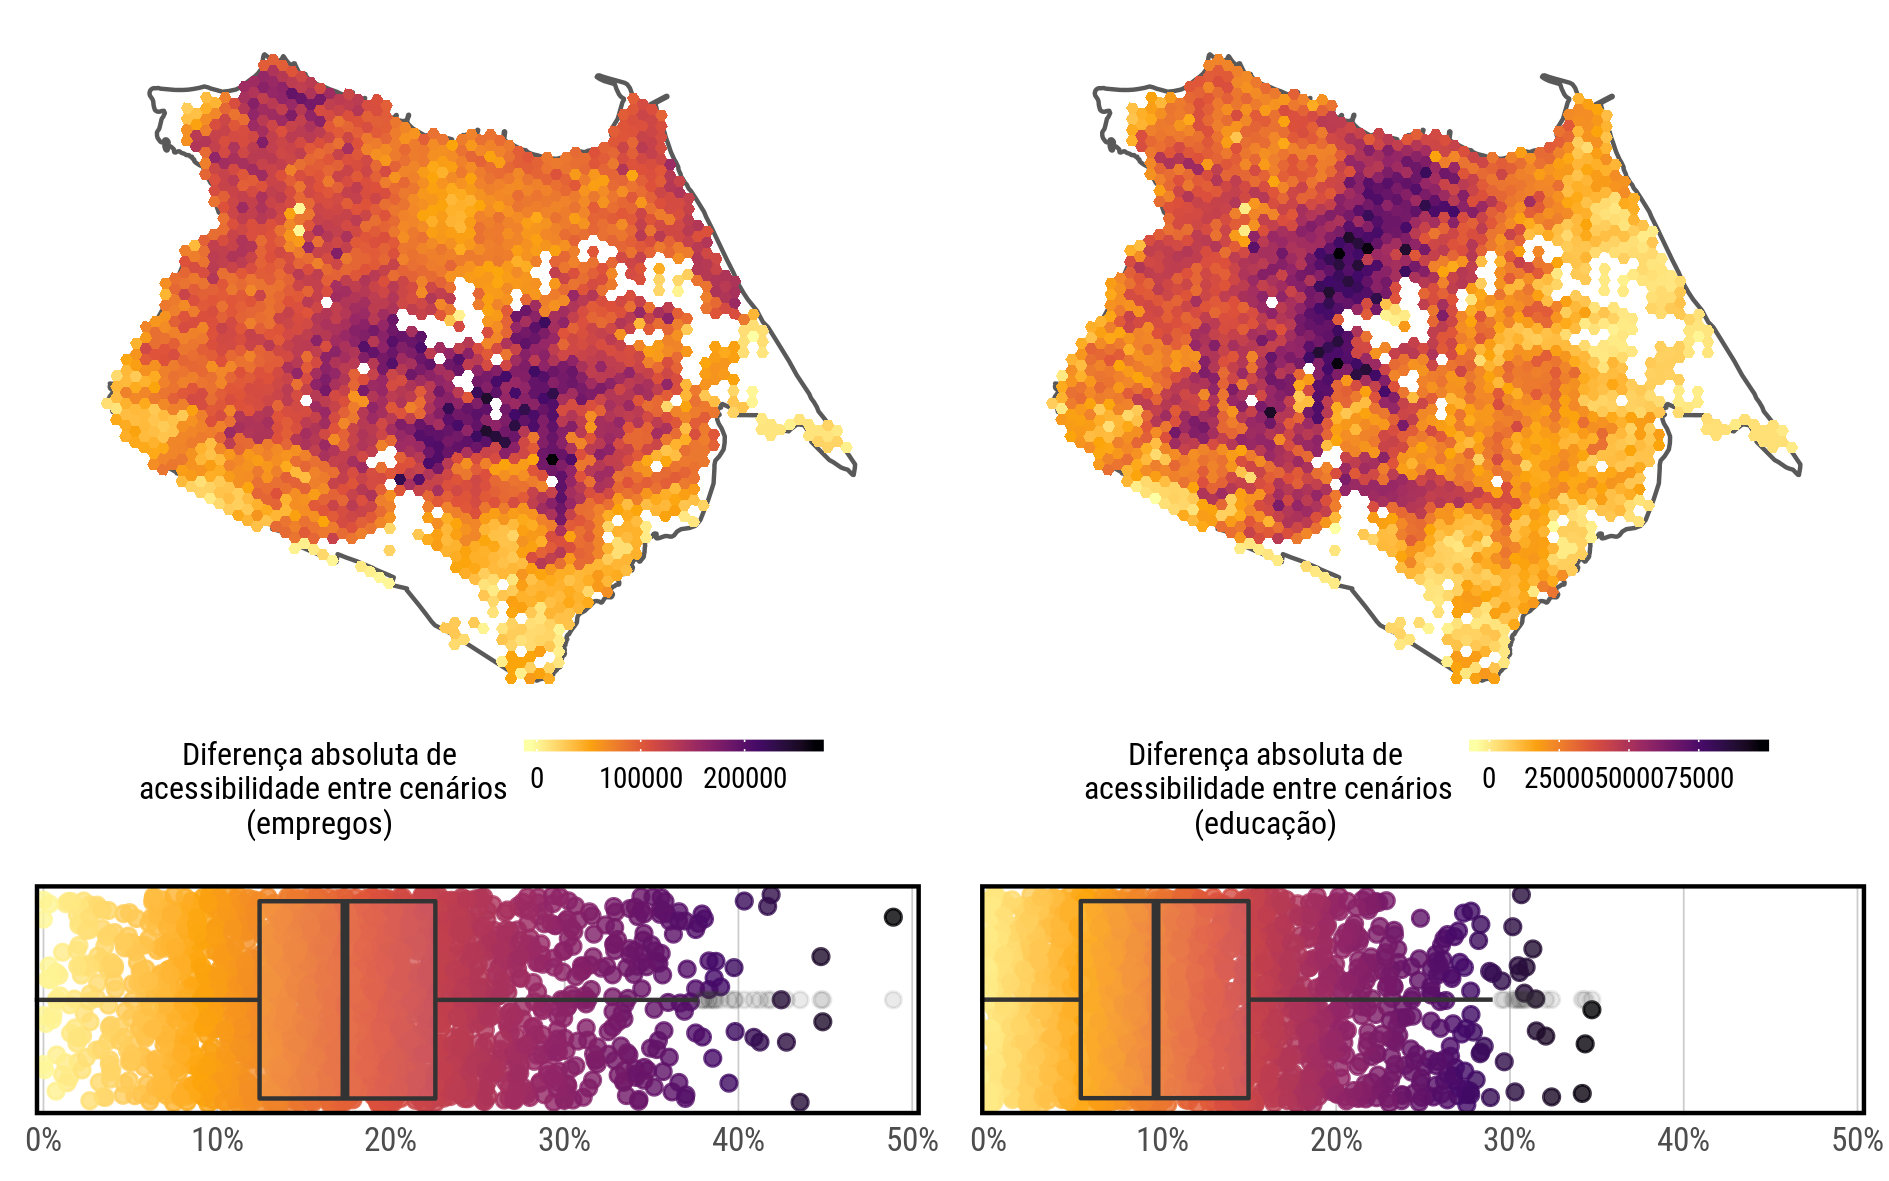
\includegraphics[width=16cm, keepaspectratio]{figure/5-acess_dif_cenarios.png}}
  }{
  \Fonte{Elaborada pelo autor}
  }
  \end{figure}
  
  Assim como na Figura \ref{fig:h1_abs}, os \emph{boxplots} da Figura \ref{fig:h2_abs} mostram essa diferença em percentuais do total de atividades na cidade. A alta variabilidade dos tempos de viagem faz com que a cidade perca em média acesso a 18\% dos seus empregos e a 10\% das suas matrículas. O mesmo padrão da análise da hipótese 1 é encontrado, onde a dispersão da diferença percentual é menor para educação do que para trabalho.
  
  Para exemplificar essa variação absoluta, é analisada a diferença na área de influência entre o GTFS P50 (em azul) e o GTFS P85 (vermelho) de um hexágono crítico que tem uma diferença de 200 mil empregos acessíveis entre os cenários (Figura \ref{fig:h2_extremo}). A imprevisibilidade do sistema faz com que o morador dessa área não acesse as principais zonas de atividades da cidade, causando uma grande perda de acessibilidade. Como identificado acima, essa região está próximo da BR-116, que é a principal via de ligação da área com o centro da cidade. Frequentes congestionamentos na área podem levar usuário dessa região a ter uma grande diferença de acessibilidade.
  
  \begin{figure}[!h]
  \captionsetup{width=16cm}
  \Caption{\label{fig:h2_extremo}Áreas de influência do GTFS P50 (azul) e do GTFS P85 (vermelho) de zona crítica}
  \centering
  \UFCfig{}{
  {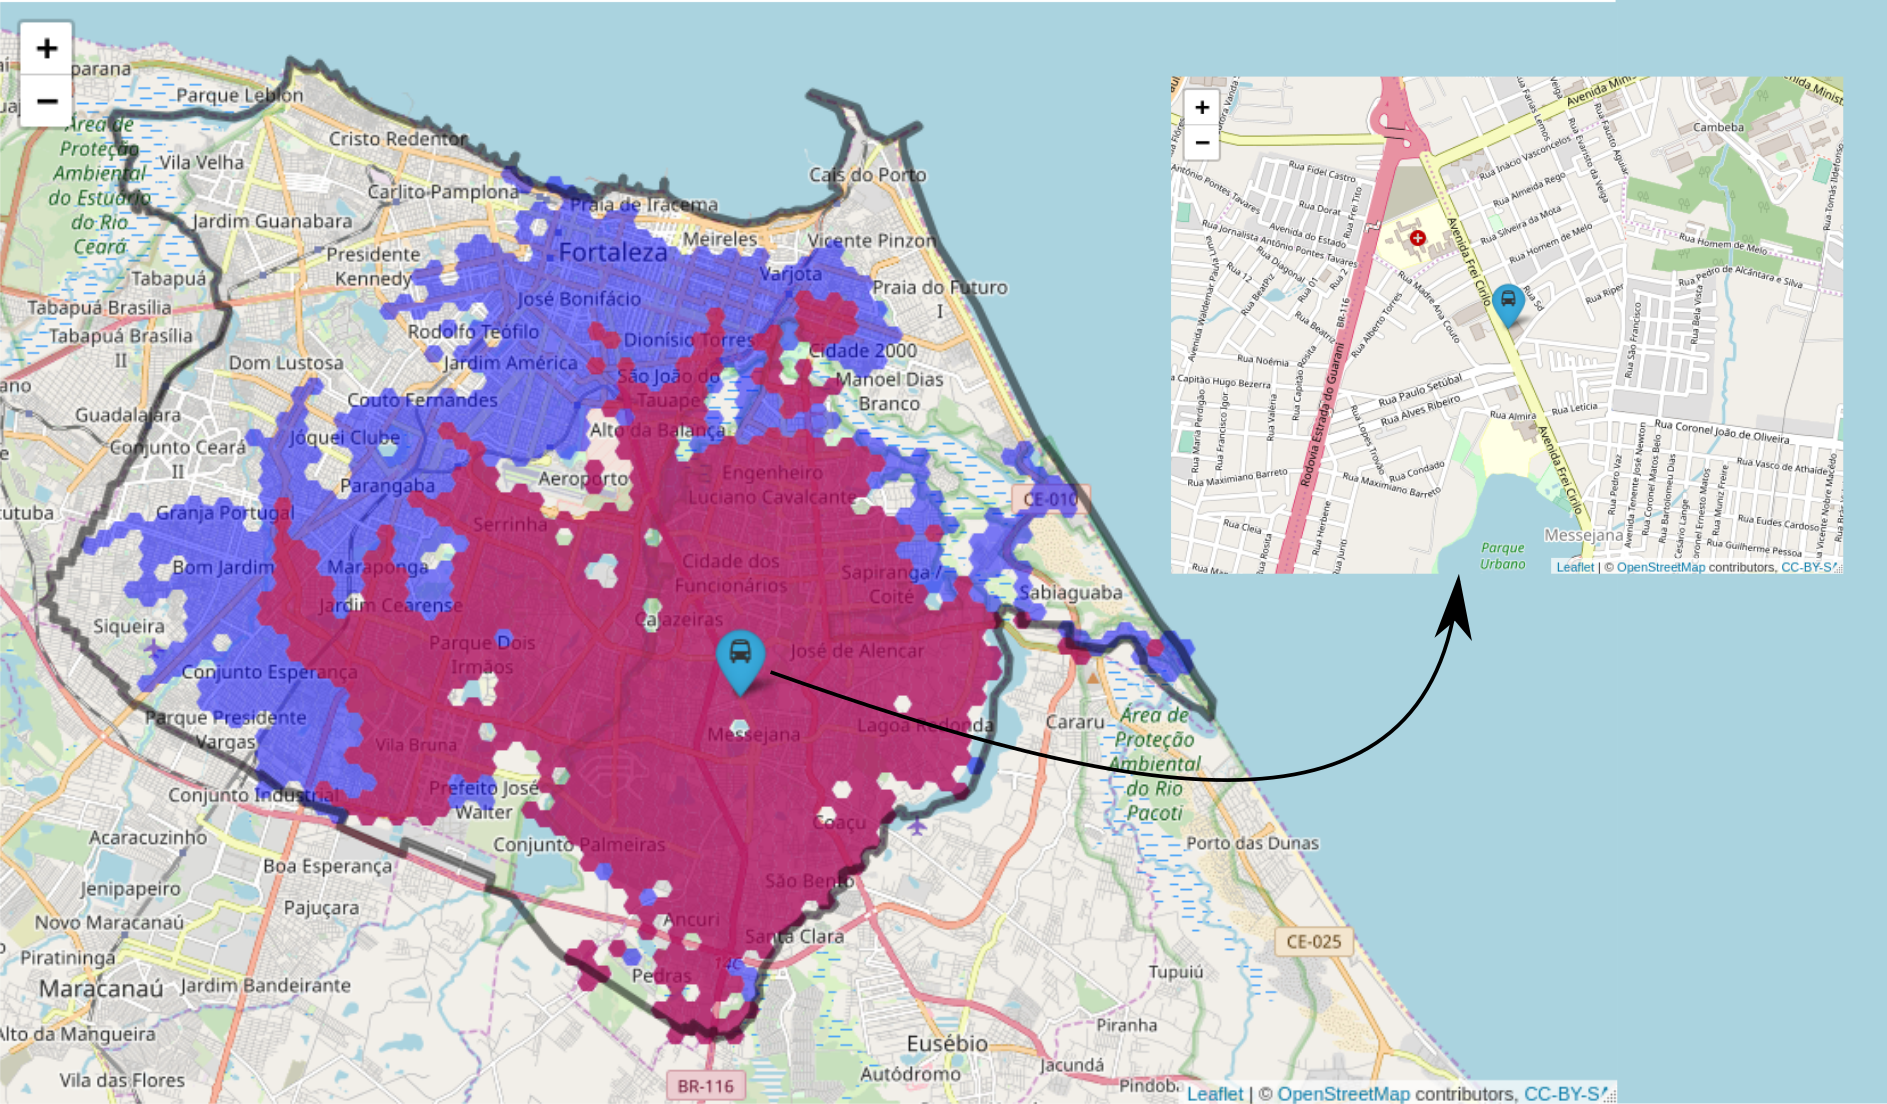
\includegraphics[width=16cm, keepaspectratio]{figure/5-acess_extremo_p50xp85_fim.png}}
  }{
  \Fonte{Elaborada pelo autor}
  }
  \end{figure}
  
  A avaliação dessa hipótese apresenta resultados conforme esperado, principalmente na visualização da acessibilidade na cidade. Um pouco inesperado, entretanto, foi o número grande na variação absoluta de oportunidades acessíveis (emprego) para algumas áreas. Foi mostrado que áreas que dependem praticamente de uma única via (BR-116) para acessar o centro da cidade podem sofrer grandes variações da acessibilidade. Isso é em função principalmente da diferença do tempo de viagem no sistema entre cenários, mas também da relação entre a localização dessas zonas e das áreas de concentração de empregos.
  
  As zonas de menor diferença absoluta de acessibilidade entre os cenários estão localizadas tanto no centro de atividades como nas zonas periféricas. Para o centro, entende-se que acontece o mesmo fenômeno que acontece na hipótese 1: é provável que os tempos de viagem entre os cenários seja significante, mas não o suficiente para que aquelas zonas deixem de acessar os locais de maior concentração de atividades dentro do tempo de 65 minutos. Para a periferia, são identificadas duas causas: primeiro, os tempos de viagem na rede em vias locais tende a variar menos que em vias troncais. Segundo, a acessibilidade dessas áreas já é pequena, com os moradores acessando poucos empregos da zona central em 65 minutos. Supõe-se que, mesmo que seja considerado um estado mais congestionado dos tempos de viagem, as áreas de concentração dos empregos continuam não sendo acessadas, resultando numa perda pequena da acessibilidade absoluta.
  
  Num cenário de proposição e avaliação de intervenções de transporte, é importante observar que a utilização dos valores centrais de tempo de viagem podem superestimar bastante a acessibilidade quando se leva em conta a dispersão dos tempos de viagem. Para uma situação de proposição de intervenções, a análise da hipótese fornece informações sobre onde as intervenções podem ser priorizadas: certas áreas estão sujeitas a grande variação na sua acessibilidade, então o aumento da capacidade e/ou a construção de infraestrutura exclusiva para transporte público terá um grande impacto. Na área de avaliação, entende-se que utilizar os valores de tempo de viagem P85 oferece uma maior segurança tanto em avaliações \emph{ex-ante} como em avaliações \emph{ex-post}. A consideração desse percentil nessas avaliações oferece uma análise de acessibilidade mais condizente com as situações de variabilidade na oferta de transporte público enfrentada pelos usuários.
  
  \hypertarget{comparacao-da-acessibilidade-para-diferentes-horas-de-partida-gtfs-p50}{%
  \section{Comparação da acessibilidade para diferentes horas de partida (GTFS P50)}\label{comparacao-da-acessibilidade-para-diferentes-horas-de-partida-gtfs-p50}}
  
  Analisando a hipótese de que a acessibilidade varia conforme o horário de partida, a Figura \ref{fig:h3_tt} mostra o valor do coeficiente de variação da acessibilidade para atividades de trabalho de cada hexágono para todos os 5 horários de partida agregados (06:45 à 07:45). A variação do coeficiente pode ir desde próximo de 0 até 0,7. Um olhar mais atento mostra que as áreas em preto (de menor variação) são concentradas na zona central de atividades e também próximas de corredores importantes de ônibus. É possível identificar duas manchas no sentido noroeste (corredor Leste-Oeste e corredor Mister Hull-Bezerra de Menezes) e duas manchas saindo do centro em direção a sudeste (corredor BR-116 e corredor Washington Soares). Todos esses corredores são caracterizados por uma grande frequência de transporte público, o que leva os usuários a esperar menos para embarcar em um veículo, aumentando a quantidade de oportunidades acessíveis. No sentido oposto, zonas no extremo leste e algumas no sentido sul mostra a importância da frequência na acessibilidade. A distribuição não-espacial mostra um coeficiente de variação mediano de aproximadamente 12\%, com o percentil 25 de 5,6\% e o percentil 75 de 21\%.
  
  \begin{figure}[!h]
  \captionsetup{width=16cm}
  \Caption{\label{fig:h3_tt}Coeficiente de variação da acessibilidade para atividades de trabalho para diferentes horas de partida}
  \centering
  \UFCfig{}{
  {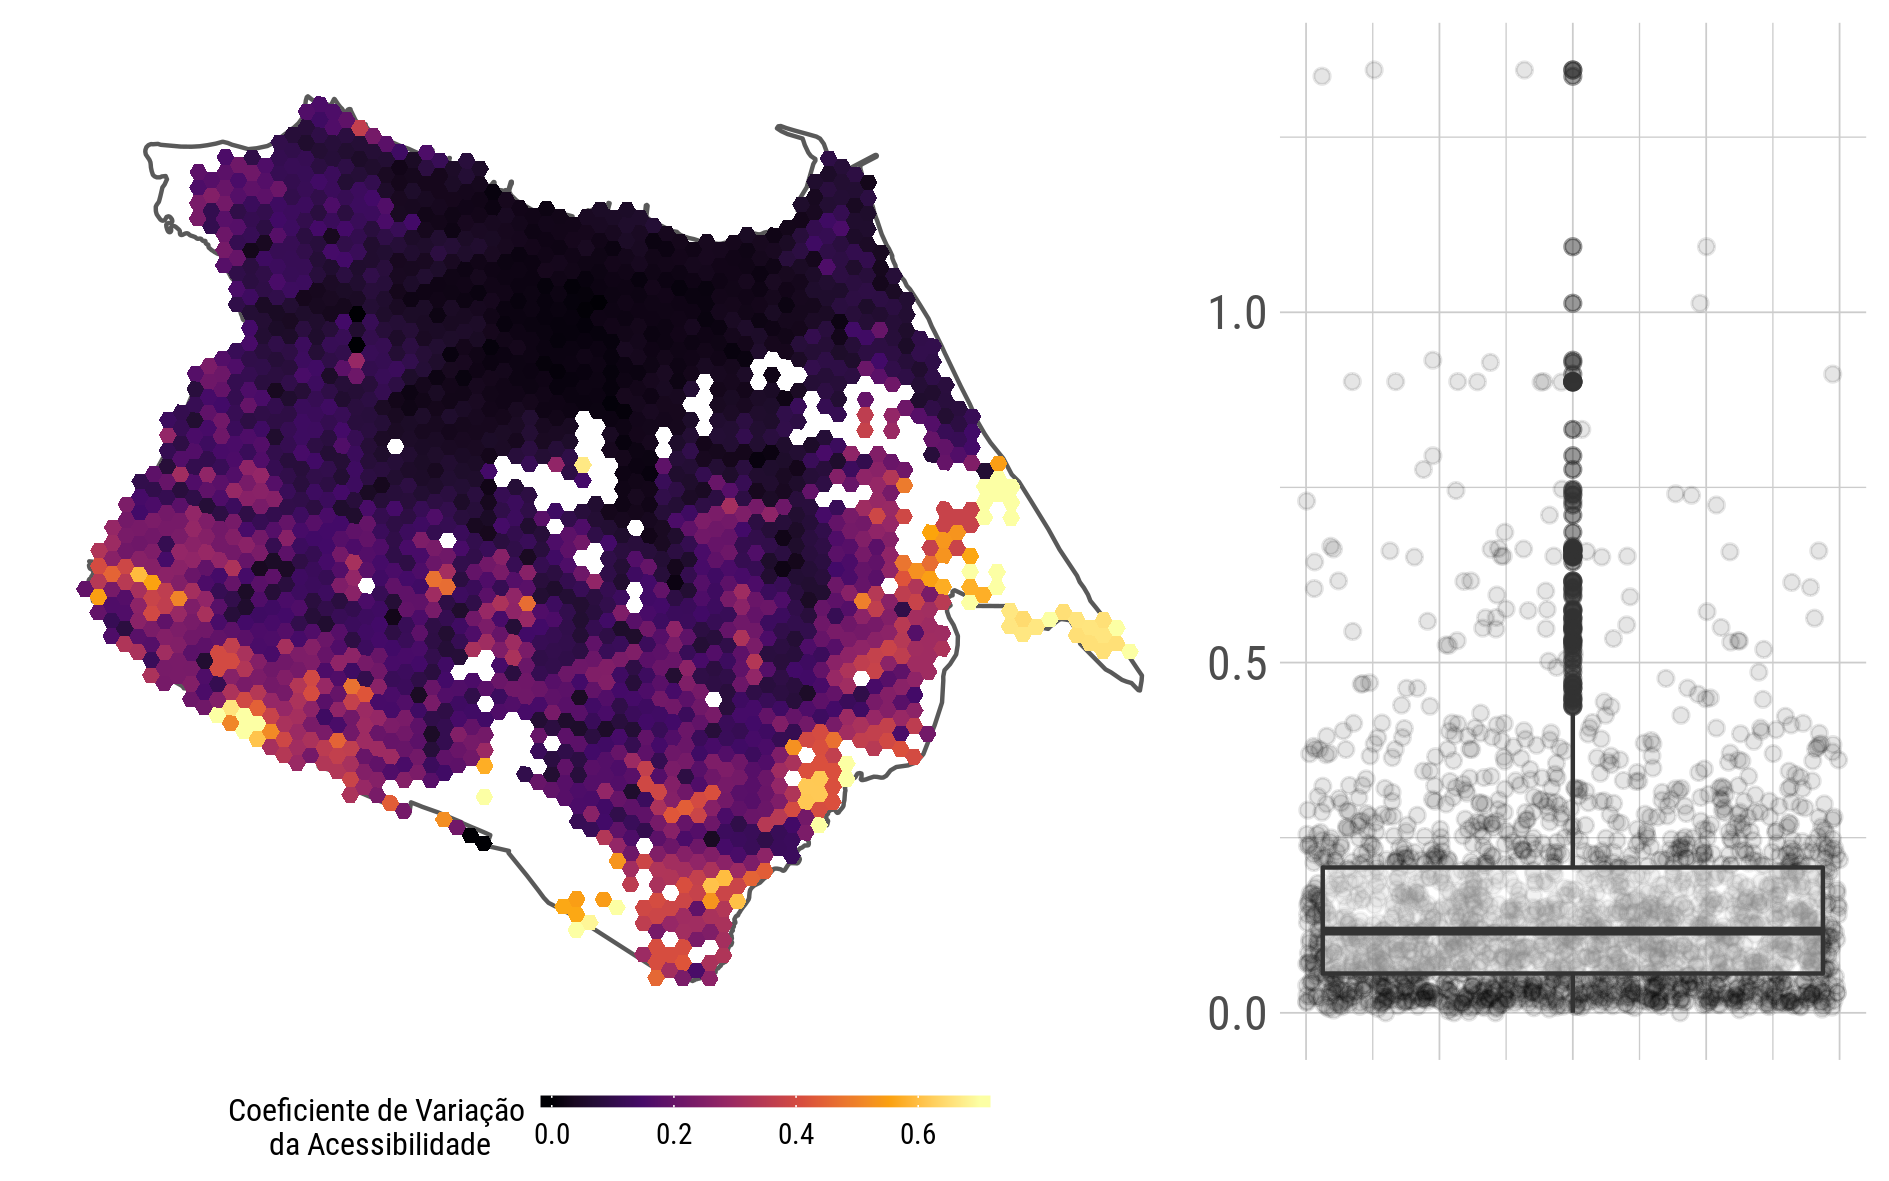
\includegraphics[width=16cm, keepaspectratio]{figure/5-cv_acess_tt_horas.png}}
  }{
  \Fonte{Elaborada pelo autor}
  }
  \end{figure}
  
  Para as atividades de educação (Figura \ref{fig:h3_et}), é identificado que a manchas mais escuras (com menor coeficiente de variação) estão presentes mais nas regiões oeste e sul da cidade, onde estão a maior parte das oportunidades. Como esperado, a variação é maior em zonas mais afastadas, e tende a aumentar com uma maior distância dos corredores de transportes. A distribuição não-espacial mostra uma variação bem semelhante à encontrada para ao indicador para trabalho, com uma mediana de 13\% de coeficiente de variação.
  
  \begin{figure}[!h]
  \captionsetup{width=16cm}
  \Caption{\label{fig:h3_et}Coeficiente de variação da acessibilidade para atividades de educação para diferentes horas de partida}
  \centering
  \UFCfig{}{
  {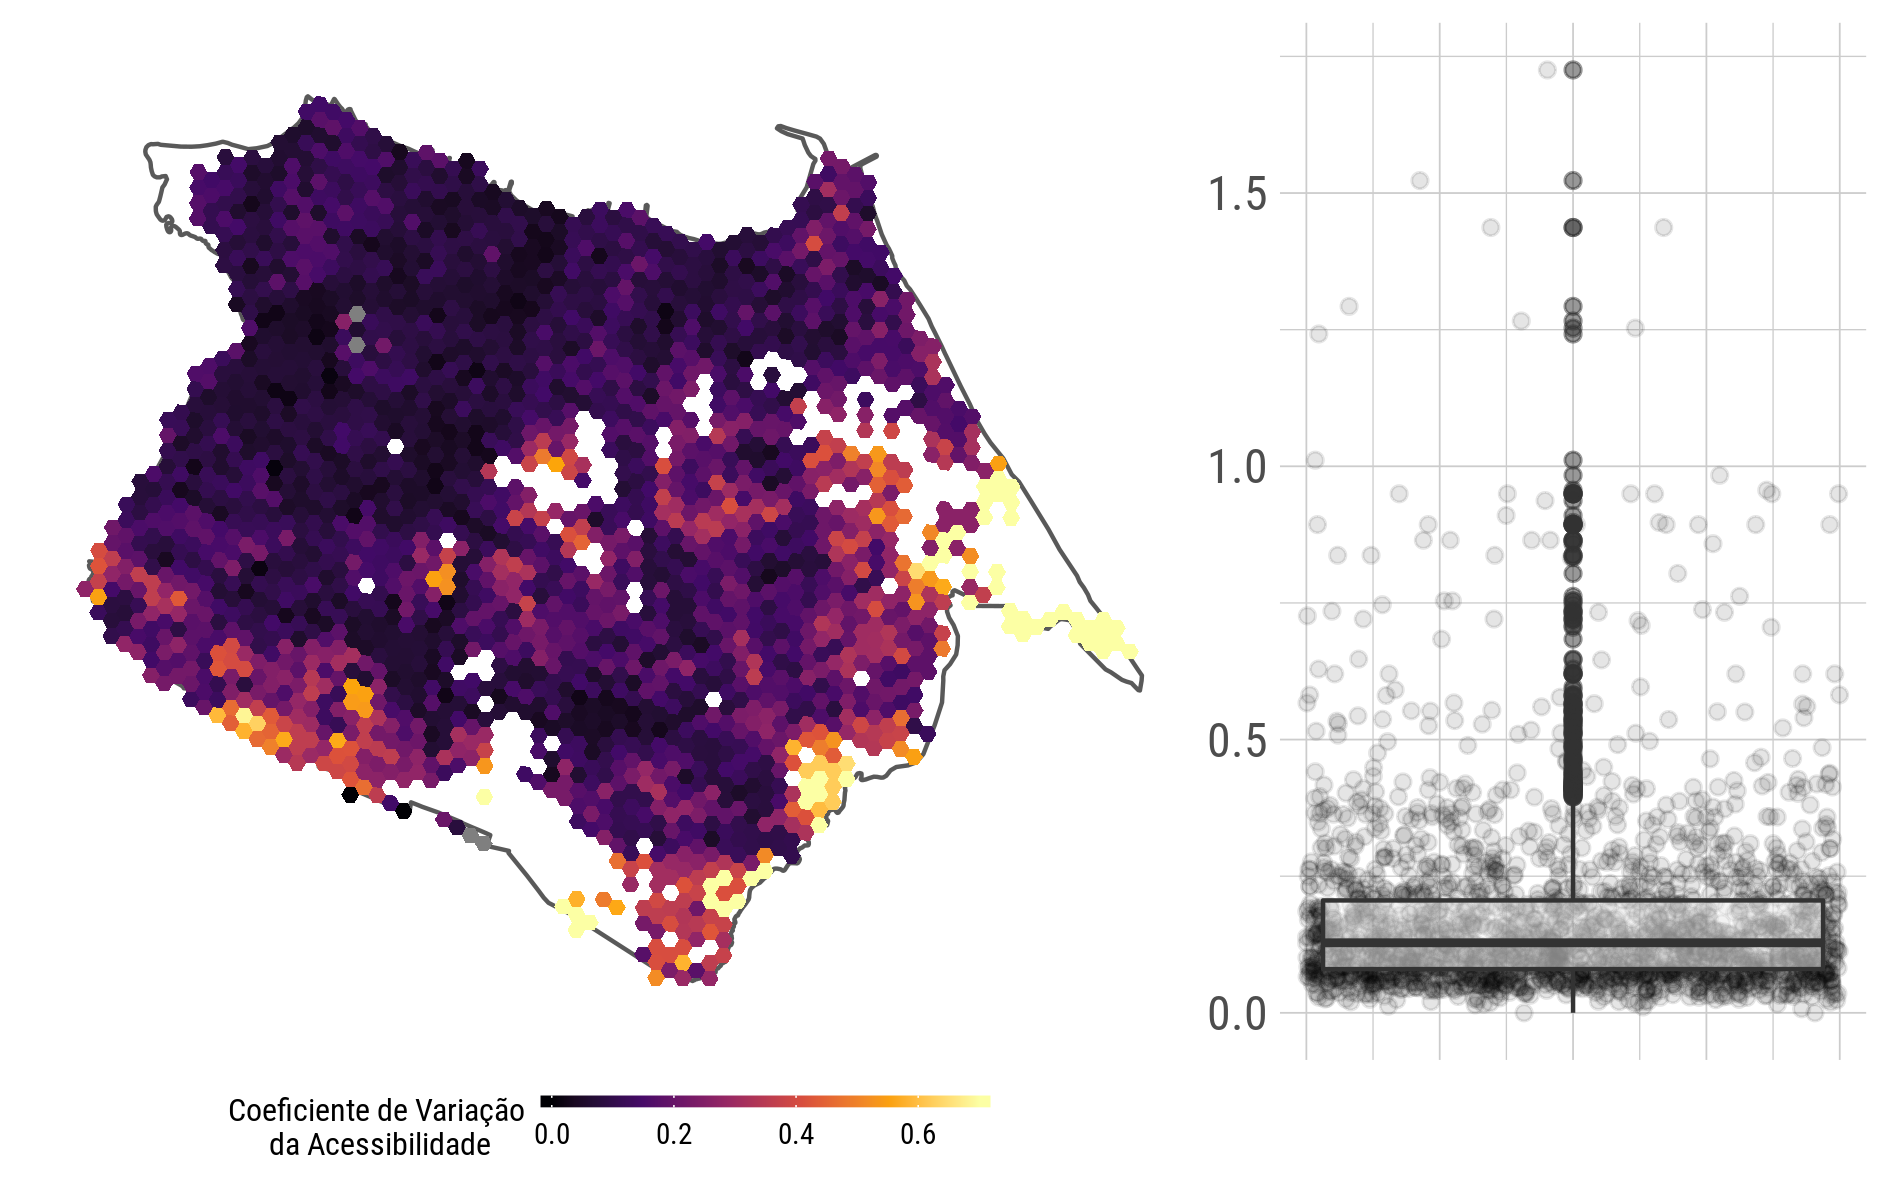
\includegraphics[width=16cm, keepaspectratio]{figure/5-cv_acess_et_horas.png}}
  }{
  \Fonte{Elaborada pelo autor}
  }
  \end{figure}
  
  Para o tomador de decisão, as análise realizadas primeiramente mostram a importância que a frequência tem na variabilidade da acessibilidade. Essas informações podem guiar novas intervenções de aumento de frequência em áreas mais afastadas, por exemplo. Entretanto, é importante ressaltar que, na realidade, grande parte dos usuários vão ajustar seu horário de saída da residência para a chegada do veículo baseado na sua experiência. Esse ajuste, entretanto, depende muito da variabilidade do serviço, o que nos leva à análise feita na hipótese 2.
  
  Num contexto de análise das intervenções, o teste da hipótese mostra a importância de se levar em consideração diversos tempos de partida nas avaliações. O impacto da utilização de poucos horários de partida na avaliação é pequeno para áreas que têm alta frequência de transporte público, mas pode ser decisivo para áreas de baixa frequência.
  
  \hypertarget{comparacao-com-resultados-encontrados-na-literatura}{%
  \section{Comparação com resultados encontrados na literatura}\label{comparacao-com-resultados-encontrados-na-literatura}}
  
  Como visto nas Figuras \ref{fig:resultado_correcao_gtfs} e \ref{fig:resultado_otp}, há uma simetria entre horários programados x corrigidos e tempos estimados entre pares de origem destino a partir do GTFS Programado x GTFS Corrigido. Esse resultado é semelhante ao encontrado pelo trabalho de \citet{Wessel2019}, que fez a mesma avaliação para quatro sistemas de transporte público diferentes da América do Norte.
  
  Os resultados encontrados para a hipótese 1, em geral, seguem o que foi encontrado no trabalho de \citet{Wessel2017}. Na questão da acessibilidade, uma comparação espacial é comprometida porque a agregação de \citet{Wessel2017} é de setores censitários, que são bem mais agregados do que os hexágonos aqui utilizados. Além disso, os autores também utilizaram uma escala percentual para medir a diferença relativa. Dito isso, para a acessibilidade para empregos, há uma distribuição semelhante de valores positivos e valores negativos, com algumas aglomerações encontradas. Não é possível comparar valores da distribuição dessa diferença porque os autores não disponibilizaram essas informações.
  
  Para a hipótese 3, os valores encontrados aqui corroboram os valores encontrados no trabalho de \citet{Owen2015}. Os autores utilizaram uma resolução temporal bem maior (uma matriz por minuto, n = 120), o que permitiu coletar resultados mais consistentes, especialmente para aáreas de baixa frequência de serviço. Lá, também foi encontrado que coeficientes de variação da acessibilidade tendem a ser menores em zonas com uma alta frequência de transporte público e maiores em zonas mais remotas. Mais uma vez, o zoneamento utilizado foi de setores censitários, onde não é possível visualizar a variação desse coeficiente em torno de corredores.
  
  A comparação com o encontrado na literatura para essas duas hipóteses só foi possível para atividades de emprego, visto que foi essa a atividade que os trabalhos analisaram. Para oportunidades de educação, essas distribuições tendem a variar mais, levantando à questão de como esses mesmo indicadores se comportariam para essa atividade em diferentes cidades. No que diz respeito à hipótese 2, não foi encontrado um trabalho que tenha se proposto a analisar a variação da acessibilidade em virtude da dispersão do tempo de viagem dos veículos.
  
  \hypertarget{conclusoes-e-recomendacoes}{%
  \chapter{Conclusões e recomendações}\label{conclusoes-e-recomendacoes}}
  
  Esse trabalho de mestrado teve como objetivo geral analisar a variabilidade de indicadores de acessibilidade por transporte público às oportunidades cumulativas de trabalho e educação com o uso de big data no contexto da avaliação de intervenções no sistema de transportes. Esse objetivo geral foi dividido em cinco objetivos específicos de pesquisa.
  
  O primeiro objetivo disse respeito à consolidação e integração dos dados de transporte público de Fortaleza. No capítulo 3 foi mostrado que a integração das bases era falha: havia falta de correspondência entre bilhetagem, GPS e GTFS para diversas linhas e veículos. Isso ocasionou uma limitação que deveria ser reconhecida para a etapa do estabelecimento da metodologia. Por fim, dados de bilhetagem, GPS, GTFS e cadastro dos usuários foram prontos para o desenvolvimento do método que viria em seguida.
  
  O segundo objetivo tratou do estabelecimento de uma método para a reconstrução de horários programados de transporte público para tendo em vista as hipóteses estabelecidas e as limitações encontradas nos dados consolidados e integrados. Esse objetivo foi atingido no primeiro tópico do capítulo 4, denominado de integração entre o GPS e GTFS, já olhando para as suas aplicações para a estimação da acessibilidade.
  
  O método apresentado para a reconstrução das viagens agendadas do GTFS a partir de dados arquivados de GPS permitiu fazer essa reconstrução quando não se tem os dados populacionais do rastreamento da frota. Primeiramente, foi necessário transformar os dados de GPS (registros a cada 30s de quase todos os veículos do transporte público) em uma tabela de horários de passagem em cada parada. Para isso, foram necessárias três etapas principais: a definição das viagens, a definição do sentido da viagem e a estimação do momento de passagem em cada parada.
  
  Na primeira etapa, foi proposto um método que apresentava avanços em relação aos demais métodos encontrados na literatura, considerando o tempo total de viagem do veículo e o tempo que ele gastou com embarques/desembarques entre uma viagem e outra. Na segunda etapa, o método não foi diferente do que foi adotado na literatura. Na terceira, foi proposta uma interpolação linear na rede para a estimação do momento de passagem de cada veículo em cada parada programada, o que foi entendido como um avanço em relação aos método anteriores que só interpolam quando a parada não era estimada. A aplicação dessas três etapas permite então a criação de uma tabela de horários em cada parada para todos os veículos que puderem ser estimados.
  
  Sabendo que essas tabelas de horários não representavam todas as linhas e veículos, foi então proposta uma agregação das mesmas. Para isso, todos os horários de passagem foram agregados para os trechos entre paradas e intervalos de 15 minutos mais próximos. Essa agregação, buscando avaliar o efeito da variação do tempo de viagem do sistema na acessibilidade, foi feita para duas medidas: a mediana dos tempos de viagem (P50) e o percentil 85 (P85). Então, para cada trecho percorrido em cada intervalo de 15 minutos, teve-se como resultado uma coluna informando o tempo mediano e uma coluna informando o tempo do percentil 85 do tempo de viagem no trecho e intervalo.
  
  A etapa da reconstrução da tabela de horários \emph{stop\_times.txt} utilizou uma amostra de dados de GPS que foi advinda da etapa de consolidação. Essa amostra já contava com a exclusão de algumas linhas integralmente (principalmente linhas complementares) e outras parcialmente. Na agregação descrita acima, 17\% dos trechos e intervalos tiveram uma amostra menor que 10 observações de tempo de viagem, e foram deletadas. Essas duas situações de descarte de amostra tendem a ter um viés, visto que ocorrem em locais periféricos de menor frequência. Para esses casos (trechos) onde não foi possível estimar o tempo de viagem, foi utilizado o valor programado do GTFS. Isso pode ser identificado como a principal limitação nessa etapa do trabalho.
  
  Os três últimos objetivos buscavam comprovar a importância do método estabelecido, e para isso foram testadas três hipóteses para acessibilidade por transporte público: 1) há diferença entre a acessibilidade estimada pelo GTFS Programado em relação ao GTFS Corrigido (P50); 2) há diferença entre a acessibilidade estimada pelos tempos de viagem medianos (P50) e de percentil 85 (P85); 3) há diferença entre a acessibilidade para diferentes tempos de partida de viagem. O método estabelecido anteriormente foi então aplicado para 1 mês de registro de GPS de Fortaleza, com a posterior aplicação de um algoritmo para a estimação do tempo de viagem entre cada par origem-destino para cada GTFS produzido e para 5 horários de partida em hora pico (05:45, 06:00, 06:15, 06:30 e 06:45).
  
  Essas hipóteses foram então testadas para acessibilidade para trabalho e educação com o uso de um indicador cumulativo de oportunidades. Foi proposta a utilização dos dados de bilhetagem para a estimação do tempo limite a ser utilizados nos indicadores. A partir desses dados foram estimadas as origens e destinos das viagens por motivo trabalho (viagens feitas com vale transporte) e por motivo educação (viagens feitas com carteira de estudante). Utilizando a mediana dos tempos de viagem calculados entre pares-origem destino do OTP, foi então calculada a distribuição dos tempos de viagem realizados para viagens por vale transporte e carteira de estudante. Por fim, os percentis 75 desses tempos foram utilizados para definir os tempos limites, resultando em 65 minutos para trabalho e 50 minutos para educação. Os indicadores de acessibilidade foram então estimados.
  
  Foi encontrado que, para a hipótese 1, a acessibilidade estimada para trabalho com o uso do GTFS Programado superestima a acessibilidade na maioria das agregações espaciais, com uma mediana da diferença de acessibilidade relativa entre os cenários de 3,5\%. Em certas áreas, a diferença absoluta pode chegar a mais de 100 mil empregos superestimados (caso fosse usado o GTFS Programado). Para as atividades de educação, por conta do diferente padrão de distribuição dessas oportunidades na cidade, a dispersão da diferença relativa tende a ser menor, com uma mediana de 3\% para a subestimação com o uso do GTFS Programado.
  
  Para a hipótese 2, primeiramente foi observado visualmente que há uma diferença de acessibilidade para empregos entre os cenários P50 e P85. Em seguida, foi mapeado a diferença absoluta de acessibilidade que a imprevisibilidade do sistema pode causar: há uma aglomeração de hexágonos que possui diferenças de até 200 mil empregos acessíveis para os cenários diferentes. Foi mostrado como isso acontece a partir da análise de uma agregação individualmente, mostrando que essa grande diferença de acesso absoluto acontece porque o sistema de transportes mais carregado (P85) leva o usuário a deixar de acessar as principais zonas de empregos da cidade (dentro do tempo limite de 65 minutos).
  
  Por fim, a hipótese 3 foi testada através do cálculo do coeficiente de variação da acessibilidade para empregos e educação para os horários de partida (n = 5 para hora pico). Foi mostrado que a variação tende a aumentar quando se distancia dos corredores de ônibus e de zonas de alta frequência de serviço. Isso indica que a frequência tem um papel importante na acessibilidade, diminuindo consideravelmente o tempo de espera dos usuários.
  
  Os resultados encontrados mostram a importância que os horários empíricos e sua dispersão tem na variabilidade da acessibilidade quando a distribuição de diferentes atividades são levadas em consideração. As atividades de trabalho são mais concentradas no centro da cidade, o que ocasiona um grande fluxo no sentido periferia-centro, que leva a altos e imprevisíveis tempos de viagens por transporte público. Assim, os veículos têm uma pontualidade menor (causando os resultados mostrados na hipótese 1) e uma variabilidade no tempo de viagem maior (causando os resultados mostrados na hipótese 2). Quando as atividades de educação são consideradas, acontece uma inversão no cenário. Essas atividades, menos concentradas na região central, assumem fluxos de acesso em sentidos opostos ao do pico trabalho da manhã, resultando em vias de acesso menos congestionadas e mais previsíveis. Isso é refletido na avaliação da hipótese 2 para essa atividade: a maior pontualidade dos veículos leva a uma menor variação entre os cenários.
  
  A análise das hipóteses finalizou com a demonstração de como as variações encontradas na acessibilidade podem impactar os tomadores de decisões em avaliações de intervenções de transporte. Foi argumentado que o uso de horários programados ou o uso de horários empíricos medianos podem levar à superestimação de intervenções baseadas em métricas de acessibilidade. Indo adiante, a utilização desses dados também pode levar a decisões equivocadas de intervenções, optando por alternativas que não levem em consideração a falta de previsibilidade do sistema.
  
  Espera-se que estudos futuros que utilizem dados de GTFS para estimar acessibilidade busquem incorporar dados empíricas de tempo de viagem a partir do rastreamento da frota, seja para melhorar a qualidade da estimação ou para estudar a variabilidade (tanto de tempo de viagem como de tempo de partida). Senão, que pelo menos reconheçam as limitações que a utilização de um GTFS Programado impõe.
  
  O método foi proposto pensando na sua replicação para diferentes realidades. Entretanto, algumas considerações precisam ser feitas sobre como esse método pode ser utilizado para outros conjuntos de dados.
  
  \hypertarget{sobre-a-reprodutibilidade-do-metodo}{%
  \section{Sobre a reprodutibilidade do método}\label{sobre-a-reprodutibilidade-do-metodo}}
  
  O método desenvolvido neste trabalho contou com bases de dados de GPS, bilhetagem, GTFS e cadastro dos usuários do sistema de transporte público de Fortaleza. Os dados continham alguns inconsistências e informações faltantes, então primeiramente foi necessário consolidá-los e integrá-los.
  
  O método proposto no capítulo 4, então, parte de dados consolidados de transporte público, e o seu funcionamento para dados de outras cidades depende disso. É sabido, entretanto, que enquanto dados de GTFS são dados padronizados (e métodos utilizados neste trabalho devem funcionar para qualquer outra caso), dados de bilhetagem e GPS podem variar significativamente.
  
  Uma das diferenças na metodologia desta dissertação diz respeito ao uso de dados arquivados de GPS. Dados arquivados de GPS tendem a ser mais problemáticos, imperfeitos, e com informações faltantes. Isso foi mostrado, por exemplo, no trabalho de \citet{Arbex2016} para os dados de São Paulo e através de uma rápido análise dos dados de GPS do Rio de Janeiro, Brasil. Essa amostra de situações, mesmo pequena, levou a crer que dados arquivados de outras cidades do Brasil ou do mundo sigam o mesmo padrão de qualidade.
  
  Portanto, do lado dos dados de GPS, o método é inteiramente reproduzível caso o dado tenha informações básicas como a linha, hora, veículo e localização. Caso o dado já tenha informação do sentido da viagem, é necessário pular essa etapa na metodologia e seguir adiante para as demais etapas de estimação do momento de passagem em cada parada, etc.
  
  Com os dados de GPS checados, é importante também ressaltar a importância de dados confiáveis de GTFS. No método desenvolvido, a integração das bases requer que a grande maioria das linhas estejam operando de acordo com o previsto no GTFS, ou seja, que estejam respeitando o itinerário, que sigam a devida ordem de paradas e que terminem e comecem suas viagens nos pontos previstos. Qualquer descompasso em relação a essa integração pode levar com que a estimação dos tempos de viagem naquela linha sejam parcialmente/totalmente descartados. Devido ao bom trabalho realizado pela ETUFOR, os dados de GTFS apresentavam uma boa conformidade com o que era executado, resultando num grande aproveitamento da amostra. É entendido, entretanto, que outros dados de GTFS não tenham o mesmo padrão de qualidade, e/ou que o sistema na realidade não siga o planejado.
  
  Ainda em relação aos dados de GTFS, neste trabalho foram adotadas duas premissas para a correção: a primeira viagem de cada veículo é correta e a oferta programada (quantidade de veículos) das linhas é correta. Por meio de conversas e apresentação de dados por parte do gestores foi possível concluir que essas premissas são factíveis. Porém, entende-se que essa não é a realidade para outras cidades. Nesse caso, recomenda-se que a tabela \emph{stop\_times} do GTFS seja recomposta exatamente com a oferta observada de um dia ou mais nos arquivos de GPS (como foi feito por \citet{Wessel2017}). Evidente que para isso é necessário que o dado de GPS compreenda todas as viagens realizadas no sistema (que não foi o caso do SIT-FOR).
  
  Os dados de GTFS de Fortaleza são do tipo \emph{stop\_times}, que contam com uma tabela de horários do transporte público. Outro tipo de GTFS, baseado em um arquivo \emph{frequency}, são ainda mais aproximados e sujeitos a erros que os anteriores. O arquivo \emph{frequency} apresenta informações de frequência programada da linha (headway previsto), e os tempos de viagem entre as paradas das linhas são considerados os mesmo para todos os horários. Nesse caso, é necessário construir completamente o arquivo \emph{stop\_times}, não somente reconstruir. Assim, a contribuição dos dados de GPS é maior ainda.
  
  Espera-se também que os códigos disponibilizados no Github sirvam para facilitar a reprodutibilidade do método. É necessário algum conhecimento na linguagem de programação R para poder adaptar diferentes casos para o código desenvolvido para Fortaleza, mas entende-se que uma pessoa com um conhecimento intermediário seja capaz de reproduzi-lo.
  
  \hypertarget{qualidade-e-disponibilidade-de-dados-de-transporte-publico}{%
  \section{Qualidade e disponibilidade de dados de transporte público}\label{qualidade-e-disponibilidade-de-dados-de-transporte-publico}}
  
  O principal problema dessa pesquisa diz respeito à integração das diversas bases de transporte público. Como foi visto na etapa de consolidação, as duas principais bases (bilhetagem e GPS) apresentavam identificadores únicos de veículo com numerações diferentes. Para localizar as validações ou para estimar a linha do GPS, é necessário que esses números tenham correspondência. Existe uma base que permite fazer essa integração, mas que acaba deixando muitos veículos de fora. Essa falha na integração faz com que o big data represente agora uma amostra do sistema, e não a mais a população diária tanto dos dados da demanda como dos dados da oferta. E uma amostra, claro, sempre trás consigo um viés, que não foi analisado neste trabalho.
  
  Passada a primeira etapa na integração, a segunda etapa também traz alguns problemas: há algumas linhas faltantes na base de GTFS. Algumas operações como estimar corretamente a parada de embarque dos usuário ou filtrar espacialmente registros de GPS de uma linha não são possíveis caso a linha em questão não exista na base do GTFS. Há outras formas de contornar isso, mas que também trazem consigo muita imprecisão. Tendo em vista o restante do método, uma linha faltante do GTFS comprometeria uma análise daquela linha de qualquer forma porque não teria como corrigir uma tabela de horários inexistente.
  
  A partir dessas observações, recomenda-se aqui uma maior ação dos responsáveis pelas bases de dados (ETUFOR e M2M) no que diz respeito a sua integração. Bases de dados com identificadores únicos iguais permitiriam inclusive uma maior facilidade na integração para pesquisadores que não sejam muito proficientes em ferramentas de manipulação de dados.
  
  Apesar dessa problemática, é necessário identificar que a disponibilização e coleta de todos os dados (big data) de transporte público do SIT-FOR não representou um problema para essa pesquisa. Os dados foram disponibilizados numa parceria da Prefeitura de Fortaleza com a Universidade Federal do Ceará, mas a prefeitura também tem um portal de dados abertos de transporte público (\url{http://dados.fortaleza.ce.gov.br/catalogo/organization/etufor}), mesmo que desatualizado. Essa não é a realidade para a grande parte das cidades brasileiras. Muitos municípios têm relutância em compartilhar dados de transporte público, especialmente dados de bilhetagem, que podem apresentar informações da demanda, e esse tipo de política acaba comprometendo pesquisas na área
  
  \hypertarget{recomendacoes-futuras-para-trabalhos-academicos}{%
  \section{Recomendações futuras para trabalhos acadêmicos}\label{recomendacoes-futuras-para-trabalhos-academicos}}
  
  A aplicação do método de integração dos dados de GPS com GTFS apresentou alguns subprodutos que oferecem oportunidades para trabalhos futuros. Dados de tempo de viagem entre paradas já foram utilizados por \citet{Arbex2016} para fazer análises ex-post da implementação de corredores de ônibus. Para o SIT-FOR, \citet{Rabay2017} já analisou velocidade operacionais entre segmentos constantes de via, mas se reservou a analisar poucas linhas. Recomenda-se, portanto, a utilização desse subproduto para uma análise mais completa da velocidade operacional do sistema.
  
  Outras análises possíveis com uma extensão do método são análises ex-ante do impacto que intervenções no transportes tem na acessibilidade. A alteração de parâmetros e adição de linhas aos arquivos GTFS permitem responder perguntas como: Qual o impacto na acessibilidade do aumento da frequência de uma linha de metrô? Qual o impacto da adição de uma linha de BRT para a acessibilidade da cidade? A integração do GTFS e OTP para a estimação de tempos de viagens entre pares origem-destino permite responder essas perguntas de forma mais ágil e integrada. A utilização dos hexágonos H3 de alta resolução permite visualizar tendências que são invisíveis em outras agregações espaciais. Para o Rio de Janeiro, o trabalho de \citet{Pereira2019} tratou de responder algumas dessas perguntas. Recomendam-se trabalhos com essa temática para o SIT-FOR, principalmente utilizando o método mais detalhado de output do OTP.
  
  A parte de resultados do trabalho teve um foco maior em mostrar a importância do método que foi proposto. São recomendados estudos que se aprofundem na análise da acessibilidade principalmente de duas temáticas levantadas: 1) no impacto do horário de partida na acessibilidade e 2) no impacto da variabilidade da oferta (tempo de viagem) na acessibilidade. Para o primeiro, recomenda-se principalmente aumentar o tamanho da amostra de hora de partida coletados. A amostra coletada aqui foi de 5 momentos de partidas, que é considerado pequena, ainda assim mostrando como a frequência do serviço interfere na acessibilidade. Para o segundo, recomenda-se uma análise mais detalhadas de pontos críticos da cidade que tem sua acessibilidade afetada pela alta variabilidade na oferta do transporte público. Recomenda-se, por fim, estudos que analisem com uma maior precisão estatística as diferenças tanto na acessibilidade por horário de partida como nos cenários de variabilidade. Perguntas que podem ser feitas incluem: os resultados são estatisticamente diferentes? Há um efeito da espacialidade nessas diferenças? Qual o seu tamanho?
  
  Recomenda-se também a replicação do método de integração do GPS e GTFS para dados de outras cidades. O método foi feito pensando em dados arquivados de GPS, mas é possível que existam outros tipos de dados com outras limitações. A tentativa de replicação do método permitirá a adaptação do método para outros dados, aumentando seu alcance.
  
  Outra sugestão de trabalho futuro é a estimação da acessibilidade baseado nas limitações de tempo/espaço de cada usuário de transporte público. Existem métodos consolidados na literatura \citep{Trepanier2007, Munizaga2012} que estimam o diário de deslocamento para cada usuário do transporte público (quais deslocamentos foram feitos? Em quais linhas? Quanto tempo levou?), e, junto a dados de gênero e idade desses usuários, esses diários podem ser utilizados para avaliar a acessibilidade considerando as restrições temporais/sociais/comportamentais impostas a esses grupos. Dessa forma, algumas hipóteses de restrição de acessibilidade podem ser estudadas, como:
  
  \begin{itemize}
  \tightlist
  \item
    Idosos tendem a caminhar menos e buscar rotas mais seguras que podem levar a tempos de viagem superiores, o que pode diminuir sua acessibilidade;
  \item
    Mulheres tendem a fazer mais viagens encadeadas que homens (deixar filhos na escola, fazer compras etc), o que pode diminuir sua acessibilidade às demais atividades;
  \item
    Pessoas que gastam muito tempo no deslocamento ao trabalho têm pouco tempo restante para acessar atividades de educação e de lazer.
  \end{itemize}
  
  Alguns desafios para esse tipo de análise podem ser encontrados. O SIT-FOR, no seu sistema tronco-alimentador, apresenta terminais de integração fechados onde os usuários que chegam de ônibus não precisam validar para embarcar em outro ônibus. Isso significa que na base da bilhetagem muitos usuários terão trechos da sua viagem que não serão registrados. Os métodos de estimação do diário de deslocamento dos usuários comumente desenvolvidos não abordam esse tipo de falta de informação. Portanto, é necessário desenvolver (ou adaptar) os métodos existentes para incorporar a realidade do SIT-FOR, podendo assim estimar cada etapa do deslocamento e partir para as análises de acessibilidade.
  
  Além disso, muitas das restrições de acessibilidade à oportunidades enfrentadas por mulheres, por exemplo, podem não ser refletidas no seu diário de deslocamento no transporte público. Pode ser levantada a hipótese, por exemplo, que mulheres tem restrição de acessibilidade porque gastam mais tempos que os homens fazendo viagens encadeadas como levando o filho a pé à escola, por exemplo. Por isso pode ser interessante juntar o diário dos deslocamentos por transporte público com pesquisas domiciliares ou dados do censo que contenham informações pessoais sobre deslocamentos diários.
  
  Este trabalho também esboçou uma discussão sobre o conceito de acessibilidade normativa x acessibilidade positiva proposto por \citet{Paez2012}, e propôs uma metodologia e aplicou o conceito positivo com o uso dos dados de bilhetagem. A aplicação buscou estimar o tempo de viagem do percentil 75 para viagens motivo trabalho e educação, partindo da hipótese que o tempo reservado para as atividades era diferente. A hipótese, que foi confirmada, também abre espaço para a estratificação desse conceito tanto para renda, idade, local de residência ou gênero.
  
  Outra potencialidade dos dados de bilhetagem na acessibilidade positiva é na calibração de modelos gravitacionais. O diário detalhado de viagem dos usuários permite o cálculo de uma matriz origem destino dos deslocamentos por transporte público. Essa informação pode subsidiar a estimação de indicadores de acessibilidade potenciais que utilizam o método gravitacional.
  
  \hypertarget{recomendacoes-futuras-para-o-poder-publico}{%
  \section{Recomendações futuras para o poder público}\label{recomendacoes-futuras-para-o-poder-publico}}
  
  Primeiramente, é necessário reconhecer o papel ainda incipiente da acessibilidade no planejamento urbano feito pelo poder público. Enquanto o conceito é consolidado e aplicado em países da Europa e da América do Norte, poucos casos são conhecidos para cidades brasileiras. O planejamento para a acessibilidade é de certa uma forma uma evolução do planejamento da mobilidade, outrora focado na diminuição do tempo de viagem, de congestionamentos etc. O planejamento da acessibilidade parte do entendimento da cidade como um sistema complexo de interação entre o sistema de transportes e uso do solo. A principal recomendação nesse aspecto é que o poder público mude o foco do seu planejamento.
  
  A utilização de subprodutos do método também pode ser útil para o poder público. Esses dados permitem analisar trechos que têm baixa velocidade operacional, ou que tendem a ter uma grande variabilidade. Isso dá informações precisas de onde são necessárias infraestruturas para a priorização do transporte público, por exemplo.
  
  Os dados consolidados de bilhetagem apresentam a sua localização, e estas podem ser alocadas à parada mais provável de embarque dos usuários. A agregação das validações por paradas pode fornece informações das paradas mais carregadas do sistema, e podem ser avaliadas intervenções que busquem otimizar e tornar mais confortável o uso da infraestrutura. Um exemplo de intervenção pode ser de pegar as paradas mais carregadas do sistema e criar uma infraestrutura diferenciada para pedestres e ciclistas em volta delas, melhorando as condições de first e last mile.
  
  No que diz respeito à acessibilidade, recomenda-se que o setor público olhe principalmente para áreas que apresentaram uma alta variação de acessibilidade em virtude 1) da hora de partida 2) da variabilidade dos tempos de viagem. Essas áreas precisam de intervenções que tanto aumentem a frequência de veículos como diminuam a influência da variabilidade.
  
  %Elementos pós-textuais	
	\bibliography{lib/library.bib}


\end{document}

